\documentclass[11pt,a4paper]{article}

% ========================================
% PACKAGES
% ========================================
\usepackage[utf8]{inputenc}
\usepackage[T1]{fontenc}
\usepackage{lmodern}  % Better font support for larger sizes
\usepackage[english]{babel}  % Change to your language
\usepackage[margin=2.5cm]{geometry}

% Mathematics
\usepackage{amsmath, amssymb, amsthm}
\usepackage{mathtools}

% Graphics and colors
\usepackage{graphicx}
\usepackage{xcolor}
\usepackage{tikz}
\usetikzlibrary{positioning, arrows.meta, shapes.geometric, shapes.misc, calc}
\usepackage{pgfplots}
\pgfplotsset{compat=1.18}
\usepackage[most]{tcolorbox}

% Lists and formatting
\usepackage{enumitem}
\usepackage{parskip}
\usepackage{fancyhdr}

% Code listings (if needed)
\usepackage{listings}
\usepackage{algorithm}
\usepackage{algorithmic}

% CJK support for Chinese, Japanese, Korean characters
\usepackage{CJKutf8}

% Hyperlinks
\usepackage{hyperref}
\hypersetup{
    colorlinks=true,
    linkcolor=blue,
    urlcolor=blue,
    citecolor=blue
}

% Set table of contents depth to show only parts and sections
\setcounter{tocdepth}{0}

% ========================================
% THEOREM ENVIRONMENTS
% ========================================
\theoremstyle{definition}
\newtheorem{definition}{Definition}[section]
\newtheorem{example}{Example}[section]
\newtheorem{exercise}{Exercise}[section]

\theoremstyle{plain}
\newtheorem{theorem}{Theorem}[section]
\newtheorem{lemma}[theorem]{Lemma}
\newtheorem{proposition}[theorem]{Proposition}
\newtheorem{corollary}[theorem]{Corollary}

\theoremstyle{remark}
\newtheorem*{remark}{Note}
\newtheorem*{observation}{Observation}

% ========================================
% CUSTOM COMMANDS
% ========================================
\newcommand{\R}{\mathbb{R}}
\newcommand{\N}{\mathbb{N}}
\newcommand{\Z}{\mathbb{Z}}
\newcommand{\Q}{\mathbb{Q}}
\newcommand{\C}{\mathbb{C}}

% ========================================
% HEADER AND FOOTER
% ========================================
\setlength{\headheight}{14pt}
\pagestyle{fancy}
\fancyhf{}
\lhead{\leftmark}
\rhead{ML\&DL}
\cfoot{\thepage}
\renewcommand{\sectionmark}[1]{\markboth{#1}{}}

% ========================================
% TABLE OF CONTENTS DEPTH
% ========================================
\setcounter{tocdepth}{2} % Show only parts, sections, and subsections

% ========================================
% DOCUMENT INFORMATION
% ========================================
\title{\textbf{Machine Learning \& Deep Learning}\\
\large Artificial Intelligence}
\author{Jacopo Parretti}
\date{I Semester 2025-2026}

% ========================================
% DOCUMENT
% ========================================
\begin{document}

% Custom title page
\begin{titlepage}
    \begin{center}
        \vspace*{2cm}
        
        % University/Course info at top
        {\large\textsc{Artificial Intelligence}}
        
        \vspace{0.4cm}
        \textcolor{blue!60!black}{\rule{0.5\textwidth}{1pt}}
        
        \vspace{2.5cm}
        
        % Main title with modern spacing
        {\fontsize{36}{44}\selectfont\bfseries Machine Learning \&\\[0.5cm] Deep Learning}
        
        \vspace{1.5cm}
        
        % Subtitle with clean design
        \begin{tcolorbox}[
            colback=blue!3!white,
            colframe=blue!40!black,
            width=0.6\textwidth,
            arc=1mm,
            boxrule=0.8pt,
            left=15pt,
            right=15pt,
            top=10pt,
            bottom=10pt
        ]
            \centering
            {\large\textit{Lecture Notes}}\\[0.3cm]
            \textcolor{gray}{Master's Program in Artificial Intelligence}
        \end{tcolorbox}
        
        \vfill
        
        % Clean course details
        \begin{tcolorbox}[
            enhanced,
            colback=white,
            colframe=gray!30,
            width=0.5\textwidth,
            arc=0mm,
            boxrule=0.5pt,
            left=20pt,
            right=20pt,
            top=12pt,
            bottom=12pt,
            shadow={2mm}{-2mm}{0mm}{black!10}
        ]
            \centering
            {\small\textcolor{gray!70}{\textbf{ACADEMIC YEAR}}}\\[0.4cm]
            {\Large 2025--2026}
        \end{tcolorbox}
        
        \vspace{2cm}
        
        % Author
        {\LARGE\textsc{Jacopo Parretti}}
        
        \vspace{1.5cm}
        
    \end{center}
\end{titlepage}

\newpage
\tableofcontents
\newpage

\part{Introduction to Machine Learning}

\section{What is Machine Learning?}

Machine Learning is a branch of Artificial Intelligence that enables software to use data to find solutions to specific tasks without being explicitly programmed to do so.

\subsection{Machine Learning vs Statistical Modelling}

In traditional statistical modelling, we follow a structured process:
\begin{enumerate}
    \item Collect data
    \item Verify and clean the data (correct or discard if not clean)
    \item Use the clean data to test hypotheses, make predictions and forecasts
\end{enumerate}

In contrast, Machine Learning takes a different approach:
\begin{itemize}
    \item It is the \textbf{data} that determines which analytic techniques to use
    \item The computer uses data to \textbf{train} algorithms to find patterns and make predictions
    \item Algorithms are no longer \textbf{static} but become \textbf{dynamic}
\end{itemize}

\subsection{Conventional Programming vs Machine Learning}

The fundamental difference between conventional programming and machine learning can be understood through their inputs and outputs:

\subsubsection{Conventional Programming}
\begin{itemize}
    \item \textbf{Input}: Program + Data
    \item \textbf{Output}: Result
    \item You write the program, give it data, and get results
\end{itemize}

\subsubsection{Machine Learning}
\begin{itemize}
    \item \textbf{Input}: Data + Result
    \item \textbf{Output}: Program
    \item You give the computer data and desired results, and it learns to generate a program/algorithm
\end{itemize}

\subsection{The Machine Learning Recipe}

\begin{tcolorbox}[colback=blue!5!white,colframe=blue!75!black,title=\textbf{The 4 Fundamental Steps of ML}]
\begin{center}
Collect data $\rightarrow$ Define models $\rightarrow$ Define objective function $\rightarrow$ Minimize error
\end{center}
\end{tcolorbox}

The ML recipe consists of 4 fundamental steps:
\begin{enumerate}
    \item Collect data
    \item Define a family of possible models
    \item Define an objective (error) function to quantify how well a model fits the data
    \item Find the model that minimizes the error function (training/learning a model)
\end{enumerate}

\subsubsection{The Key Ingredients}

\begin{tcolorbox}[colback=green!5!white,colframe=green!75!black,title=\textbf{5 Essential Ingredients}]
\begin{center}
Task • Data • Model • Objective Function • Learning Algorithm
\end{center}
\end{tcolorbox}

Every machine learning problem requires five essential ingredients:
\begin{itemize}
    \item \textbf{Task}: The problem we want to solve
    \item \textbf{Data}: The information we use to learn
    \item \textbf{Model hypothesis}: The family of functions we consider
    \item \textbf{Objective function}: How we measure success
    \item \textbf{Learning algorithm}: How we find the best model
\end{itemize}

\section{Machine Learning Tasks}

A task represents the type of prediction being made to solve a problem on some data. We can identify a task with the set of functions that can potentially solve the problem. In general, it consists of functions assigning each \textbf{input} $x \in \mathcal{X}$ an \textbf{output} $y \in \mathcal{Y}$.

\subsection{Classification Task}

\begin{definition}[Classification]
Find a function $f \in \mathcal{Y}^{\mathcal{X}}$ assigning each input $x \in \mathcal{X}$ a \textbf{discrete} label, $f(x) \in \mathcal{Y} = \{c_1, \ldots, c_k\}$.
\end{definition}

In classification, the output space is a finite set of discrete categories or classes. The goal is to learn a decision boundary that separates different classes.

\subsection{Regression Task}

\begin{definition}[Regression]
Find a function $f \in \mathcal{Y}^{\mathcal{X}}$ assigning each input $x \in \mathcal{X}$ a \textbf{continuous} label, $f(x) \in \mathcal{Y} = \mathbb{R}$.
\end{definition}

In regression, the output is a continuous value, allowing for predictions of quantities such as prices, temperatures, or probabilities.

\subsection{Density Estimation Task}

\begin{definition}[Density Estimation]
Find a probability distribution $f \in \Delta(\mathcal{X})$ that best fits the data $x \in \mathcal{X}$.
\end{definition}

There is no reference to an output space (as in classification and regression tasks). Instead, we make a reasoning on the \textbf{input} $x$ itself, trying to model the underlying probability distribution that generated the data.

\subsection{Clustering Task}

\begin{definition}[Clustering]
Find a function $f \in \mathbb{N}^{\mathcal{X}}$ that assigns each input $x \in \mathcal{X}$ a \textbf{cluster index} $f(x) \in \mathbb{N}$.
\end{definition}

All points mapped to the same index form a cluster. The goal is to group similar data points together without prior knowledge of the groups.

\subsection{Dimensionality Reduction Task}

\begin{definition}[Dimensionality Reduction]
Find a function $f \in \mathcal{Y}^{\mathcal{X}}$ that \textbf{maps} each (\textbf{high-dimensional}) input $x \in \mathcal{X}$ to a \textbf{lower-dimensional} embedding $f(x) \in \mathcal{Y}$, where $\dim(\mathcal{Y}) < \dim(\mathcal{X})$.
\end{definition}

This task aims to reduce the number of features while preserving the essential information in the data.

\section{Data in Machine Learning}

\subsection{Data Representation}

We represent inputs of our algorithm as $x \in \mathcal{X}$ and outputs as $y \in \mathcal{Y}$. The dataset is the set of both, where each input is associated with an output.

\textbf{Key considerations:}
\begin{itemize}
    \item The quality of the data is crucial for the performance of the algorithm
    \item It is equally important to have a large amount of data to learn effective models
    \item Poor quality or insufficient data can lead to poor model performance
\end{itemize}

\subsection{Features}

\begin{definition}[Features]
Features are the measurable properties or characteristics of the phenomenon being observed.
\end{definition}

\textbf{Examples:}
\begin{itemize}
    \item To identify a flower: color, petal length, petal width, sepal length, sepal width
    \item To identify a fruit: color, shape, size, texture, weight
    \item To classify images: pixel values, edges, textures, shapes
\end{itemize}

We can say that features are how our algorithm "sees" the data and are in general represented with (fixed-size) vectors.

\section{Data Distributions and Learning Types}

In machine learning, the information about the problem we want to solve is represented in the form of a data distribution, usually denoted as $p_{\text{data}}$.

\subsection{Supervised Learning}

\subsubsection{Classification and Regression}

The data distribution is over pairs of inputs and outputs:
\[
p_{\text{data}} \in \Delta(\mathcal{X} \times \mathcal{Y})
\]

Here:
\begin{itemize}
    \item $\mathcal{X}$ is the input space
    \item $\mathcal{Y}$ is the output space (labels or targets)
    \item The goal is to learn a mapping from inputs to outputs using labeled data
\end{itemize}

\subsection{Unsupervised Learning}

\subsubsection{Density Estimation, Clustering, and Dimensionality Reduction}

The data distribution is only over the input space:
\[
p_{\text{data}} \in \Delta(\mathcal{X})
\]

Here:
\begin{itemize}
    \item We do not have explicit labels or targets
    \item The goal is to discover structure, patterns, or representations within the data itself
\end{itemize}

\subsection{Summary of Learning Types}

\begin{table}[h]
\centering
\begin{tabular}{|l|c|c|}
\hline
\textbf{Task Type} & \textbf{Data Distribution} & \textbf{Learning Type} \\
\hline
Classification, Regression & $p_{\text{data}} \in \Delta(\mathcal{X} \times \mathcal{Y})$ & Supervised Learning \\
\hline
Density Estimation, Clustering, & $p_{\text{data}} \in \Delta(\mathcal{X})$ & Unsupervised Learning \\
Dimensionality Reduction & & \\
\hline
\end{tabular}
\caption{Comparison of learning types based on data distribution}
\end{table}

\begin{remark}
In \textbf{supervised learning}, each data point consists of an input and a corresponding output (label). In \textbf{unsupervised learning}, each data point consists only of the input, and the algorithm tries to find patterns or structure without explicit labels.

This distinction is fundamental in machine learning, as it determines the type of algorithms and approaches used to solve different problems.
\end{remark}

\section{Data Sampling and Dataset Splitting}

\subsection{The Data Distribution Problem}

In both supervised and unsupervised learning, the true data distribution $p_{\text{data}}$ is typically \textbf{unknown}. This presents a fundamental challenge:
\begin{itemize}
    \item We do not have direct access to the underlying probability distribution that generates the data
    \item We only have access to a finite sample of data points drawn from this distribution
\end{itemize}

\textbf{Solution}: We perform \textbf{sampling} from the distribution. By collecting a representative sample of data, we can approximate the true distribution and use it to train our models.

\subsection{Training, Validation, and Test Sets}

To properly evaluate machine learning models, we split our data into three distinct sets. Each set serves a specific purpose in the machine learning pipeline.

\begin{definition}[Dataset Splitting]
A dataset is typically divided into three subsets:
\begin{itemize}
    \item \textbf{Training set} ($D_{\text{train}}$): Used to train the model
    \item \textbf{Validation set} ($D_{\text{val}}$): Used to tune hyperparameters and select the best model
    \item \textbf{Test set} ($D_{\text{test}}$): Used to evaluate the final model performance
\end{itemize}
\end{definition}

\begin{tcolorbox}[colback=yellow!10!white,colframe=yellow!75!black,title=\textbf{Critical Requirement}]
All three sets (training, validation, test) must be sampled from the \textbf{same probability distribution}
\end{tcolorbox}

\subsection{How to Use the Three Sets}

The three datasets serve different purposes in the machine learning workflow:

\subsubsection{Learning/Training Phase}

During the learning phase, the \textbf{training set} is used to train the machine learning algorithm, which learns patterns and relationships in the data to produce a \textbf{program} (model). 

The \textbf{validation set} plays a crucial role in this phase:
\begin{itemize}
    \item Evaluates different model configurations
    \item Tunes hyperparameters
    \item Selects the best performing model
\end{itemize}

This process involves iterative feedback between training and validation until we find the optimal configuration.

\subsubsection{Testing/Model Evaluation Phase}

Once the best model is selected, we use the \textbf{test set} to evaluate its performance. The trained model is applied to the test data, which it has never seen before. This gives us an unbiased estimate of how well the model will perform in real-world scenarios, telling us whether our model can truly generalize to new data.

\subsection{The Importance of Distribution Similarity}

\subsubsection{Correct Scenario: Same Distribution}

When training, validation, and test sets are sampled from the \textbf{same distribution}:
\begin{itemize}
    \item The sets are \textbf{similar} in terms of statistical properties
    \item They represent the same underlying phenomenon
    \item However, they \textbf{do not overlap} (no data point appears in multiple sets)
\end{itemize}

This ensures that the model can generalize well from training to test data.

\textbf{Example}: If we're classifying fruits, all three sets might contain apples and bananas in similar proportions, but with different specific instances.

\subsubsection{Incorrect Scenario: Different Distributions}

When training/validation and test sets come from \textbf{different distributions}, the model learns patterns from one distribution but is tested on another. This problematic scenario typically leads to:
\begin{itemize}
    \item Poor performance on the test set
    \item Unreliable predictions on new data
    \item Inability to generalize to real-world applications
\end{itemize}

\textbf{Example}: Training on apples and bananas, but testing on oranges and limes. The model cannot classify fruits it has never seen during training.

\begin{tcolorbox}[colback=orange!5!white,colframe=orange!75!black,title=\textbf{Key Principle}]
\begin{center}
Training and test data must come from the \textbf{same distribution}

Violating this leads to poor generalization
\end{center}
\end{tcolorbox}

\section{Training and Testing: The Role of Features}

\subsection{Training (Learning, Induction)}

During the training phase, the model learns to distinguish between different classes based on the features provided in the training data. 

\textbf{Example}: Consider a fruit classification task with the following training data:
\begin{itemize}
    \item \textit{red, round, leaf, 3oz, ...} $\rightarrow$ apple
    \item \textit{green, round, no leaf, 4oz, ...} $\rightarrow$ apple
    \item \textit{yellow, curved, no leaf, 8oz, ...} $\rightarrow$ banana
    \item \textit{green, curved, no leaf, 7oz, ...} $\rightarrow$ banana
\end{itemize}

The model learns to associate patterns in the features (color, shape, presence of leaf, weight) with the corresponding labels (apple or banana). \textbf{What distinguishes apples and bananas is based on the features!} The model identifies which feature combinations are characteristic of each class.

\subsection{Testing}

Once trained, the model can classify new examples based on the same features it learned during training. When presented with a new example described by the same semantic features, the model makes a prediction.

\textbf{Example}: Given a new fruit with features \textit{red, round, no leaf, 4oz, ...}, the model uses the learned patterns to predict whether it is an apple or a banana.

\begin{tcolorbox}[colback=red!5!white,colframe=red!75!black,title=\textbf{Critical Assumption}]
\begin{center}
The features of training and testing data \textbf{must be the same!}

The model can only make predictions based on features it was trained on
\end{center}
\end{tcolorbox}

\subsection{Learning and Generalization}

Learning is fundamentally about \textbf{generalizing} from the training data. The goal is not simply to memorize the training examples, but to learn patterns that apply to new, unseen data.

However, the failure of a machine learning algorithm is often caused by a \textbf{bad selection of training samples}. The key issue is that we might introduce \textbf{unwanted correlations} from which the algorithm derives \textbf{wrong conclusions}.

\textbf{Example}: Consider a model trained to recognize objects in images. If all training images were captured on sunny days, the model might learn to associate sunny weather conditions with the objects. When tested on images taken on cloudy days, the model might fail to recognize the same objects because it never encountered cloudy conditions during training. The model incorrectly learned that sunny weather is a relevant feature for object recognition.

\begin{tcolorbox}[colback=blue!5!white,colframe=blue!75!black]
\begin{center}
\textit{Quality and diversity of training data are crucial}

Training data should be representative of all real-world conditions
\end{center}
\end{tcolorbox}

\section{The Complete Machine Learning Recipe}

We can now revisit the complete machine learning workflow with all its essential ingredients:

\subsection{The Five Ingredients of Machine Learning}

Every machine learning problem requires five fundamental components that work together:

\begin{enumerate}
    \item \textbf{Task}: The specific problem we want to solve (e.g., classify birds vs. non-birds in images)
    
    \item \textbf{Data}: The collection of examples used to train and evaluate the model. Data quality and quantity are critical for success.
    
    \item \textbf{Model Hypothesis}: The family of functions or models we consider as potential solutions. This defines the space of possible models the learning algorithm can explore.
    
    \item \textbf{Objective Function}: A mathematical function that quantifies how well a model performs on the data. The learning algorithm aims to optimize this function.
    
    \item \textbf{Learning Algorithm}: The method used to search through the model hypothesis space and find the model that optimizes the objective function.
\end{enumerate}

\subsection{The Interplay of Ingredients}

These five ingredients are interconnected:
\begin{itemize}
    \item The \textbf{task} determines what kind of \textbf{data} we need and what \textbf{model hypothesis} is appropriate
    \item The \textbf{data} influences which features are available and how we define the \textbf{objective function}
    \item The \textbf{model hypothesis} constrains what the \textbf{learning algorithm} can discover
    \item The \textbf{objective function} guides the \textbf{learning algorithm} toward better models
\end{itemize}

Understanding and carefully selecting each ingredient is essential for building effective machine learning systems.

\section{Model and Hypothesis Space}

\subsection{What is a Model?}

\begin{definition}[Model]
A \textbf{model} is the implementation of a function $f \in \mathcal{F}_{\text{task}}$ that can be tractably computed.
\end{definition}

In practice, when searching for our function $f$, we don't look at everything in $\mathcal{F}_{\text{task}}$. Instead, we look at a subset called the \textbf{hypothesis space}: $\mathcal{H} \subset \mathcal{F}_{\text{task}}$, which is composed of a set of models (e.g., neural networks, decision trees, linear models).

The learning algorithm seeks a \textbf{solution within the hypothesis space}. In other words, a model is a simplified representation of the world that we can actually compute and optimize.

\begin{observation}
The choice of hypothesis space is crucial:
\begin{itemize}
    \item If $\mathcal{H}$ is too small, it may not contain a good solution
    \item If $\mathcal{H}$ is too large, finding the best model becomes computationally intractable
    \item The hypothesis space defines the types of patterns the model can learn
\end{itemize}
\end{observation}

\subsection{Types of Learning Paradigms}

\begin{tcolorbox}[colback=purple!5!white,colframe=purple!75!black,title=\textbf{Three Learning Paradigms}]
Machine learning can be categorized into different paradigms based on the type and availability of labeled data:

\subsubsection*{Supervised Learning}
In supervised learning, we have labeled data where each input is paired with its corresponding output. This includes:
\begin{itemize}
    \item \textbf{Classification}: Predicting discrete labels
    \item \textbf{Regression}: Predicting continuous values
\end{itemize}

\subsubsection*{Unsupervised Learning}
In unsupervised learning, we only have input data without labels. The goal is to discover structure in the data. This includes:
\begin{itemize}
    \item \textbf{Clustering}: Grouping similar data points
    \item \textbf{Density Estimation}: Modeling the probability distribution of data
    \item \textbf{Dimensionality Reduction}: Finding lower-dimensional representations
\end{itemize}
\end{tcolorbox}

\subsubsection{Supervised Learning}

In supervised learning, we have labeled data where each input is paired with its corresponding output.

\subsubsection{Unsupervised Learning}

In unsupervised learning, we only have input data without labels.

\subsubsection{Semi-Supervised Learning}

Semi-supervised learning addresses scenarios where we have a large amount of unlabeled data and only some labeled examples. This paradigm has gained significant popularity in recent years to leverage large datasets through self-supervised learning techniques.

The key idea is to provide the model with tasks different from the one to be solved, but that allow the model to learn the data distribution from the unlabeled data. Once the model understands the general structure of the data, it can then specialize on the few labeled examples to solve the target task.

\textbf{Example}: Training a language model on large amounts of unlabeled text to learn general language patterns, then fine-tuning it on a small labeled dataset for sentiment analysis.

\section{Model-Based vs. Instance-Based Learning}

Machine learning algorithms can be further categorized based on how they make predictions:

\subsection{Model-Based (Parametric) Learning}

\begin{definition}[Parametric Model]
A learning model that summarizes data with a \textbf{set of parameters of fixed size} (independent of the number of training examples) is called a \textbf{parametric model}.
\end{definition}

\begin{tcolorbox}[colback=cyan!5!white,colframe=cyan!75!black,title=\textbf{Parametric Model Characteristics}]
Key characteristics:
\begin{itemize}
    \item The model learns a fixed set of parameters from the training data
    \item Once trained, the original training data can be discarded
    \item No matter how much data you give to a parametric model, it won't change its mind about how many parameters it needs
    \item The model makes predictions using only the learned parameters
\end{itemize}

\textbf{Examples}: Naive Bayes, Linear Regression, Logistic Regression, Neural Networks
\end{tcolorbox}

In a model-based approach, the algorithm learns a function (e.g., a decision boundary) described by parameters. For instance, a linear classifier might learn the curve $\alpha x_1 + \beta x_2 + \gamma$ that separates two classes, where $\alpha, \beta, \gamma$ are the parameters.

\subsection{Instance-Based (Nonparametric) Learning}

\begin{definition}[Nonparametric Model]
These algorithms \textbf{do not learn parameters} but instead use the data itself to compare a new example through similarity metrics.
\end{definition}

\begin{tcolorbox}[colback=teal!10!white,colframe=teal!75!black,title=\textbf{Nonparametric Model Characteristics}]
Key characteristics:
\begin{itemize}
    \item The model stores (some or all of) the training data
    \item Predictions are made by comparing new examples to stored training examples
    \item The model's complexity can grow with the amount of training data
    \item No explicit training phase that produces a fixed set of parameters
\end{itemize}

\textbf{Examples}: K-Nearest Neighbors (KNN), Support Vector Machines (SVM), Random Forest
\end{tcolorbox}

In an instance-based approach, when a new example arrives, it is compared with nearby training examples and classified according to a similarity policy. For example, in KNN, a new point is classified based on the majority class of its $k$ nearest neighbors in the training data.

\subsection{Comparison}

\begin{table}[h]
\centering
\begin{tabular}{|l|p{5.5cm}|p{5.5cm}|}
\hline
\textbf{Aspect} & \textbf{Model-Based} & \textbf{Instance-Based} \\
\hline
Parameters & Fixed number of parameters & No fixed parameters \\
\hline
Training data & Can be discarded after training & Must be retained for predictions \\
\hline
Prediction speed & Fast (only uses parameters) & Slower (compares with stored data) \\
\hline
Memory & Low (stores only parameters) & High (stores training examples) \\
\hline
Flexibility & Fixed model complexity & Complexity grows with data \\
\hline
\end{tabular}
\caption{Comparison between model-based and instance-based learning}
\end{table}

\section{Error Function (Objective Function)}

To allow an algorithm to learn, we need to provide it with a metric, a measure that helps it understand the direction of the optimal solution we are seeking. For this reason, \textbf{performance measures} are defined to enable the algorithm to learn.

\subsection{What is an Error Function?}

In machine learning, \textbf{training a model} means finding a \textbf{function} which maps a set of values $x$ to a value $y$. We can calculate how well a predictive model is doing by comparing the \textbf{predicted values} with the \textbf{true values} for $y$.

\begin{definition}[Training Error vs. Test Error]
\begin{itemize}
    \item If we apply the model to the data it was trained on, we are calculating the \textbf{training error}
    \item If we calculate the error on data which was \textbf{unknown} in the training phase, we are calculating the \textbf{test error}
\end{itemize}
\end{definition}

The test error is the most important metric because it tells us how well the model generalizes to new, unseen data.

\subsection{Types of Error Functions}

There are different types of error functions (also called loss functions or objective functions), each suited for different tasks:

\begin{itemize}
    \item \textbf{Mean Absolute Error (MAE)}: Measures the average absolute difference between predictions and true values
    \item \textbf{Mean Squared Error (MSE)}: Measures the average squared difference between predictions and true values
    \item \textbf{Binary Cross-Entropy}: Used for binary classification problems
    \item \textbf{Mean Average Precision}: Used for ranking and information retrieval tasks
\end{itemize}

The choice of error function depends on the task and the desired properties of the model.

\section{Example: Polynomial Fitting}

Let's consider a concrete example to understand how models, hypothesis spaces, and error functions work together.

\subsection{Problem Setup}

Consider a regression problem with the following setup:
\begin{itemize}
    \item \textbf{Data}: $\mathcal{D}_n = \{(x_1, y_1), \ldots, (x_n, y_n)\}$
    \item Data generated from $\sin(2\pi x) + \text{noise}$
    \item Training set with $n = 10$ points
    \item \textbf{Goal}: Learn a function (shown as the purple line) that fits the data
\end{itemize}

The correct solution should capture the underlying sinusoidal pattern while being robust to the noise in the training data.

\begin{figure}[h]
\centering
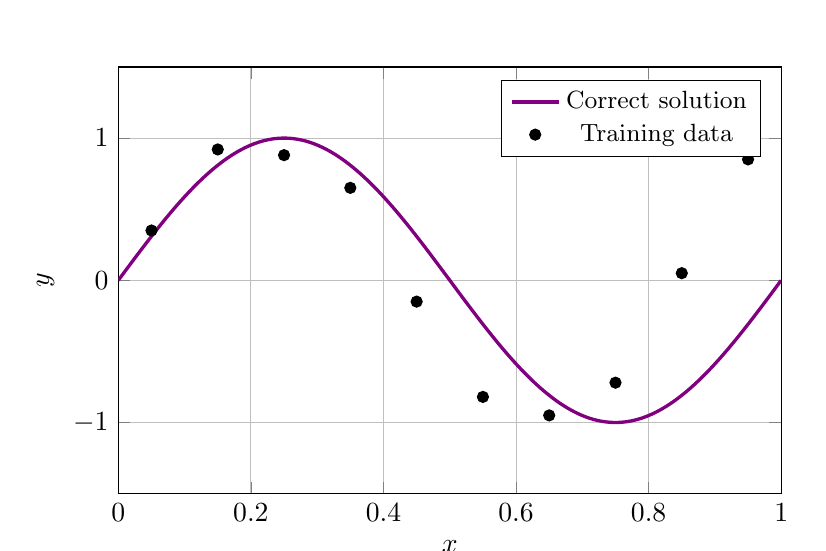
\begin{tikzpicture}
\begin{axis}[
    width=10cm,
    height=7cm,
    xlabel={$x$},
    ylabel={$y$},
    xmin=0, xmax=1,
    ymin=-1.5, ymax=1.5,
    grid=major,
    legend pos=north east,
    legend style={font=\small}
]

% True function (purple, sinusoidal)
\addplot[violet, very thick, smooth, domain=0:1, samples=100] {sin(deg(2*pi*x))};
\addlegendentry{Correct solution}

% Training data points (black dots with some noise)
\addplot[only marks, mark=*, mark size=2pt, black] coordinates {
    (0.05, 0.35)
    (0.15, 0.92)
    (0.25, 0.88)
    (0.35, 0.65)
    (0.45, -0.15)
    (0.55, -0.82)
    (0.65, -0.95)
    (0.75, -0.72)
    (0.85, 0.05)
    (0.95, 0.85)
};
\addlegendentry{Training data}

\end{axis}
\end{tikzpicture}
\caption{Polynomial Fitting Problem: Data generated from $\sin(2\pi x)$ with noise}
\end{figure}

\subsection{Model: Polynomial Functions}

\begin{tcolorbox}[colback=magenta!5!white,colframe=magenta!75!black,title=\textbf{Polynomial Model}]
We choose to model the data using polynomial functions:
\[
f_w(x) = \sum_{j=0}^{M} w_j x^j
\]

where:
\begin{itemize}
    \item $M$ is the \textbf{degree of the polynomial} (a hyperparameter)
    \item $w = \{w_0, \ldots, w_M\}$ are the \textbf{parameters} to be learned
    \item The \textbf{hypothesis space} for a fixed degree $M$ is: $\mathcal{H}_M = \{f_w : w \in \mathbb{R}^{M+1}\}$
\end{itemize}
\end{tcolorbox}

Different values of $M$ give us different hypothesis spaces:
\begin{itemize}
    \item $M = 0$: Constant functions (horizontal lines)
    \item $M = 1$: Linear functions (straight lines)
    \item $M = 2$: Quadratic functions (parabolas)
    \item $M = 3$: Cubic functions
    \item Higher $M$: More complex curves
\end{itemize}

\begin{figure}[h]
\centering
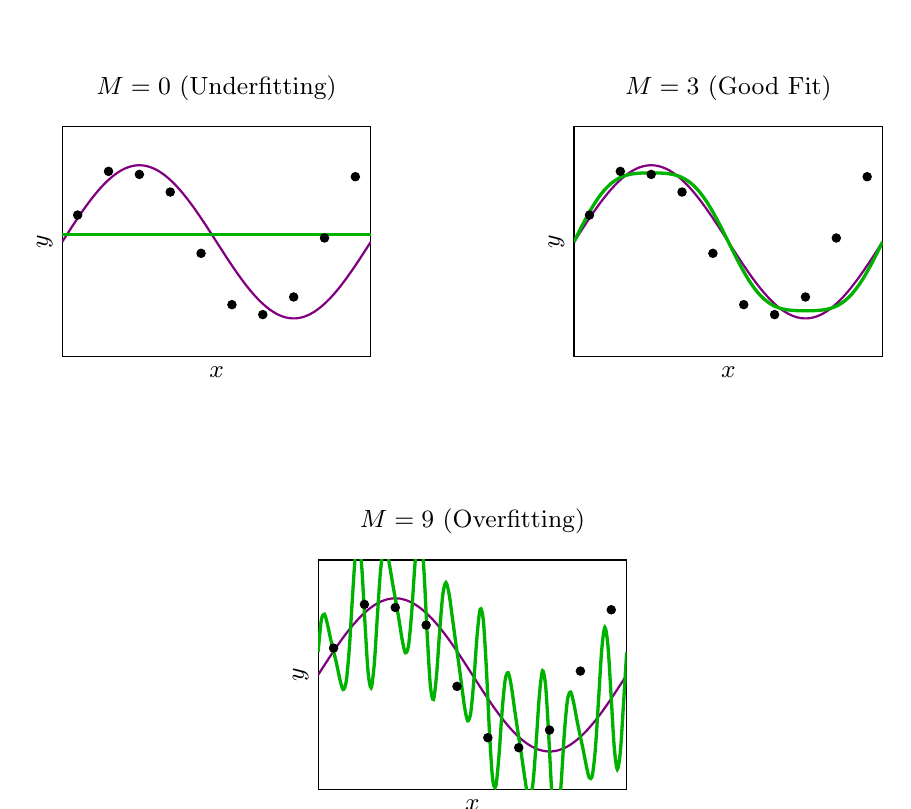
\begin{tikzpicture}

% M=0 (Underfitting)
\begin{scope}[xshift=0cm]
\begin{axis}[
    width=5.5cm,
    height=4.5cm,
    title={$M=0$ (Underfitting)},
    title style={font=\small},
    xlabel={$x$},
    ylabel={$y$},
    xlabel style={font=\small},
    ylabel style={font=\small},
    xmin=0, xmax=1,
    ymin=-1.5, ymax=1.5,
    xtick=\empty,
    ytick=\empty,
]
% Data points
\addplot[only marks, mark=*, mark size=1.5pt, black] coordinates {
    (0.05, 0.35) (0.15, 0.92) (0.25, 0.88) (0.35, 0.65) (0.45, -0.15)
    (0.55, -0.82) (0.65, -0.95) (0.75, -0.72) (0.85, 0.05) (0.95, 0.85)
};
% True function (purple)
\addplot[violet, thick, smooth, domain=0:1, samples=50] {sin(deg(2*pi*x))};
% M=0 fit (green horizontal line)
\addplot[green!70!black, very thick, domain=0:1] {0.1};
\end{axis}
\end{scope}

% M=3 (Good fit)
\begin{scope}[xshift=6.5cm]
\begin{axis}[
    width=5.5cm,
    height=4.5cm,
    title={$M=3$ (Good Fit)},
    title style={font=\small},
    xlabel={$x$},
    ylabel={$y$},
    xlabel style={font=\small},
    ylabel style={font=\small},
    xmin=0, xmax=1,
    ymin=-1.5, ymax=1.5,
    xtick=\empty,
    ytick=\empty,
]
% Data points
\addplot[only marks, mark=*, mark size=1.5pt, black] coordinates {
    (0.05, 0.35) (0.15, 0.92) (0.25, 0.88) (0.35, 0.65) (0.45, -0.15)
    (0.55, -0.82) (0.65, -0.95) (0.75, -0.72) (0.85, 0.05) (0.95, 0.85)
};
% True function (purple)
\addplot[violet, thick, smooth, domain=0:1, samples=50] {sin(deg(2*pi*x))};
% M=3 fit (green, close to true function)
\addplot[green!70!black, very thick, smooth, domain=0:1, samples=50] {sin(deg(2*pi*x)) + 0.1*sin(deg(6*pi*x))};
\end{axis}
\end{scope}

% M=9 (Overfitting)
\begin{scope}[xshift=3.25cm, yshift=-5.5cm]
\begin{axis}[
    width=5.5cm,
    height=4.5cm,
    title={$M=9$ (Overfitting)},
    title style={font=\small},
    xlabel={$x$},
    ylabel={$y$},
    xlabel style={font=\small},
    ylabel style={font=\small},
    xmin=0, xmax=1,
    ymin=-1.5, ymax=1.5,
    xtick=\empty,
    ytick=\empty,
]
% Data points
\addplot[only marks, mark=*, mark size=1.5pt, black] coordinates {
    (0.05, 0.35) (0.15, 0.92) (0.25, 0.88) (0.35, 0.65) (0.45, -0.15)
    (0.55, -0.82) (0.65, -0.95) (0.75, -0.72) (0.85, 0.05) (0.95, 0.85)
};
% True function (purple)
\addplot[violet, thick, smooth, domain=0:1, samples=50] {sin(deg(2*pi*x))};
% M=9 fit (green, oscillating wildly)
\addplot[green!70!black, very thick, smooth, domain=0:1, samples=100] {
    sin(deg(2*pi*x)) + 0.8*sin(deg(20*pi*x)) + 0.3*cos(deg(30*pi*x))
};
\end{axis}
\end{scope}

\end{tikzpicture}
\caption{Polynomial fits with different degrees: $M=0$ (underfitting), $M=3$ (good fit), $M=9$ (overfitting). Purple: true function, Green: fitted polynomial, Black dots: training data.}
\end{figure}

\subsection{Error Function: Mean Squared Error}

To measure how well our polynomial fits the data, we use the Mean Squared Error (MSE):

\[
E(f; \mathcal{D}_n) = \frac{1}{n} \sum_{i=1}^{n} [f(x_i) - y_i]^2
\]

This error function:
\begin{itemize}
    \item Computes the squared difference between the prediction $f(x_i)$ and the ground-truth label $y_i$ for each point
    \item Averages these squared differences over all $n$ training points
    \item Is also called a \textbf{pointwise loss} because it measures the error at each individual data point
\end{itemize}

The learning algorithm's goal is to find the parameters $w$ that minimize this error function:

\[
w^* = \arg\min_{w \in \mathbb{R}^{M+1}} E(f_w; \mathcal{D}_n)
\]

\begin{center}
\colorbox{cyan!10}{\parbox{0.9\textwidth}{
\textbf{Choice of Model Complexity is Crucial:}
\begin{itemize}
    \item Too small $M$: Underfitting (cannot capture pattern)
    \item Appropriate $M$: Good fit (captures underlying pattern)
    \item Too large $M$: Overfitting (fits noise, poor generalization)
\end{itemize}
}}
\end{center}

\section{Underfitting and Overfitting}

\begin{center}
\colorbox{purple!15}{\parbox{0.9\textwidth}{
\centering
\textbf{Two Fundamental Problems in ML}\\[0.2cm]
Underfitting (too simple) $\leftrightarrow$ Overfitting (too complex)
}}
\end{center}

Two fundamental problems can occur when training machine learning models: underfitting and overfitting. Understanding these concepts is crucial for building models that generalize well.

\subsection{Definitions}

\begin{definition}[Underfitting]
\textbf{Underfitting} is a scenario where a model is unable to capture the relationship between the input ($x$) and output ($y$) variables accurately, generating a high error rate on both the training set and unseen data (e.g., testing set).
\end{definition}

The model is too simple and has not yet learned from the data. It performs poorly on both training and test data.

\begin{definition}[Overfitting]
\textbf{Overfitting} occurs when the model gives accurate predictions for training data (lower training error) but not for testing data (higher testing error).
\end{definition}

The model is too sensitive to the training data and has essentially memorized it, including its noise and peculiarities, rather than learning the underlying pattern.

\subsection{The Bias-Variance Trade-off}

The relationship between model complexity, training error, and test error can be visualized as follows:

\begin{figure}[h]
\centering
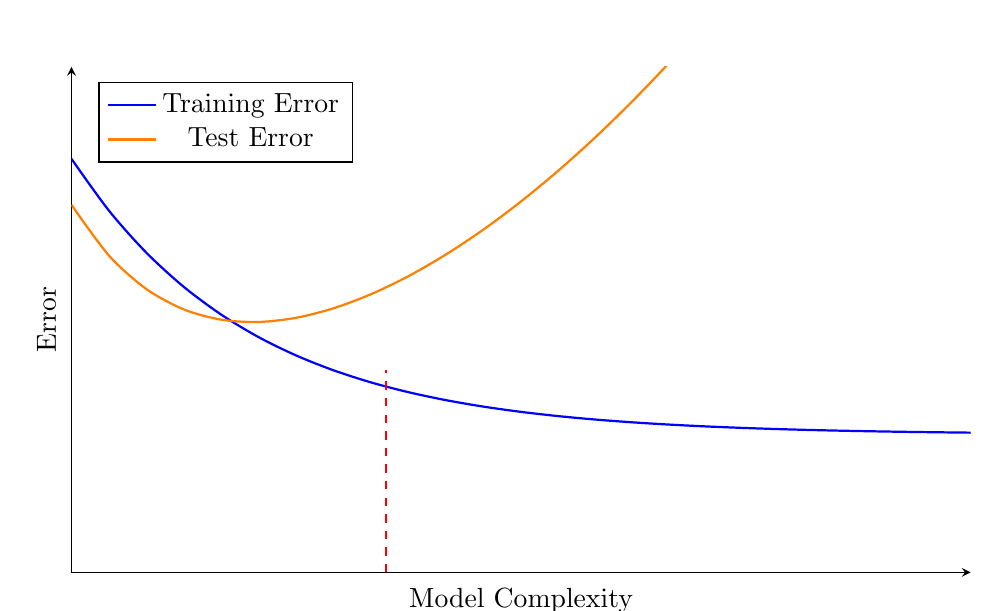
\begin{tikzpicture}
\begin{axis}[
    width=13cm,
    height=8cm,
    xlabel={Model Complexity},
    ylabel={Error},
    xmin=0, xmax=10,
    ymin=0, ymax=5.5,
    xtick=\empty,
    ytick=\empty,
    axis lines=left,
    legend pos=north west,
    legend style={font=\normalsize}
]

% Training Error curve (decreasing)
\addplot[blue, thick, smooth, domain=0:10] {1.5 + 3*exp(-0.5*x)};
\addlegendentry{Training Error}

% Test Error curve (U-shaped)
\addplot[orange, thick, smooth, domain=0:10] {2 + 2*exp(-0.8*x) + 0.08*x^2};
\addlegendentry{Test Error}

% Vertical line for "Best Fit"
\draw[red, dashed, thick] (axis cs:3.5,0) -- (axis cs:3.5,2.2);

\end{axis}
\end{tikzpicture}
\caption{Bias-Variance Trade-off: Training and Test Error vs. Model Complexity}
\end{figure}

\begin{itemize}
    \item \textbf{Left side of the graph (low complexity)}: High error rate in both training and testing $\rightarrow$ \textbf{Underfitting}
    \item \textbf{Middle region (optimal complexity)}: Low error rate in both training and testing $\rightarrow$ \textbf{Best Fit}
    \item \textbf{Right side of the graph (high complexity)}: Low error rate in training but high error rate in testing $\rightarrow$ \textbf{Overfitting}
\end{itemize}

\subsection{Diagnostic Matrix}

We can diagnose the state of our model by examining both training and test errors:

\begin{table}[h]
\centering
\begin{tabular}{|c|c|c|}
\hline
 & \textbf{Low Training Error} & \textbf{High Training Error} \\
\hline
\textbf{Low Test Error} & OK (Good fit) & Underfitting \\
\hline
\textbf{High Test Error} & Overfitting & Underfitting \\
\hline
\end{tabular}
\caption{Diagnostic matrix for model performance}
\end{table}

\subsection{How to Handle Overfitting}

When the model is too sensitive to training data and overfits, we can apply several strategies:

\begin{enumerate}
    \item \textbf{Try a simpler model}: Use a model with fewer parameters or lower complexity
    
    \item \textbf{Try a less powerful model}: Choose a model architecture with reduced capacity
    
    \item \textbf{Increase regularization impact}: Apply techniques that penalize model complexity:
    \begin{itemize}
        \item Early stopping: Stop training before the model overfits
        \item L1/L2 regularization: Add penalty terms to the loss function
    \end{itemize}
    
    \item \textbf{Use a smaller number of features}:
    \begin{itemize}
        \item Remove some features that may be causing overfitting
        \item Apply feature selection techniques to identify the most relevant features
    \end{itemize}
    
    \item \textbf{Get more data}: Increasing the training set size helps the model learn more generalizable patterns
\end{enumerate}

\subsection{How to Handle Underfitting}

When the model has not yet learned from the data and underfits, we can try:

\begin{enumerate}
    \item \textbf{Try more complex models}: Use models with a larger number of parameters that can capture more intricate patterns
    \begin{itemize}
        \item Ensemble learning: Combine multiple models
    \end{itemize}
    
    \item \textbf{Less regularization}: Reduce or remove regularization constraints that may be limiting the model's capacity
    
    \item \textbf{A larger quantity of features}: Add more features or engineer new features that better capture the underlying relationships (get more features)
\end{enumerate}

\subsection{Polynomial Fitting Example Revisited}

Let's examine how different polynomial degrees affect the fit:

\begin{itemize}
    \item \textbf{$M = 0$} (constant function): Severe underfitting. The horizontal line cannot capture any of the sinusoidal pattern. Both training and validation errors are high.
    
    \item \textbf{$M = 1$} (linear function): Still underfitting. A straight line cannot represent the curved pattern. Both errors remain high.
    
    \item \textbf{$M = 3$} (cubic polynomial): Good fit. The model captures the underlying sinusoidal pattern well. Both training and validation errors are low, and the curves are similar.
    
    \item \textbf{$M = 9$} (9th-degree polynomial): Overfitting. The model passes through all training points (very low training error) but oscillates wildly between them. The validation error is high because the model has learned the noise rather than the signal.
\end{itemize}

The error plot shows:

\begin{figure}[h]
\centering
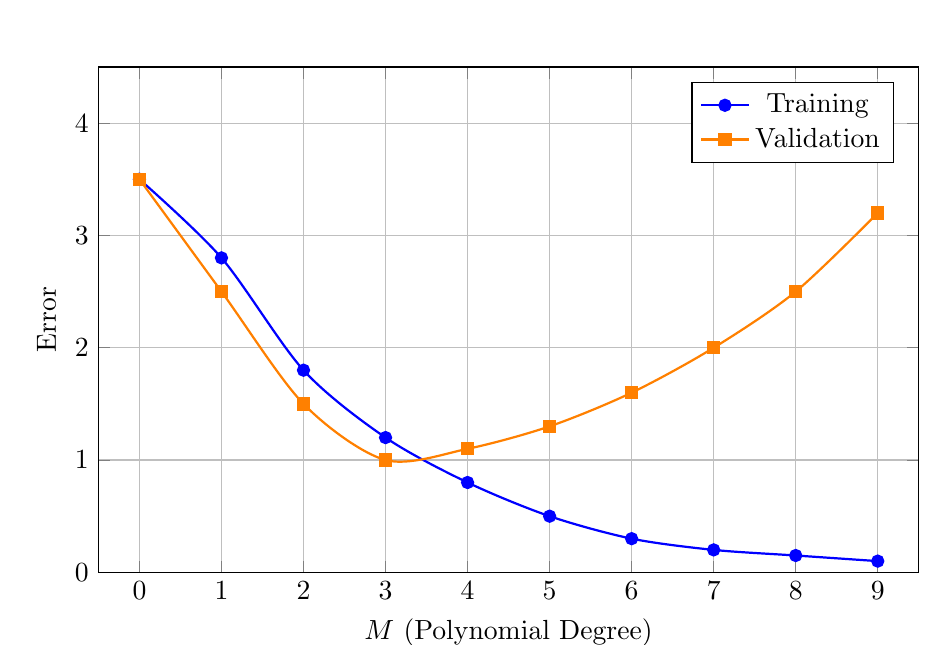
\begin{tikzpicture}
\begin{axis}[
    width=12cm,
    height=8cm,
    xlabel={$M$ (Polynomial Degree)},
    ylabel={Error},
    xlabel style={font=\normalsize},
    ylabel style={font=\normalsize},
    xmin=-0.5, xmax=9.5,
    ymin=0, ymax=4.5,
    xtick={0,1,2,3,4,5,6,7,8,9},
    grid=major,
    legend pos=north east,
    legend style={font=\normalsize}
]

% Training error (blue, decreasing)
\addplot[blue, thick, mark=*, smooth] coordinates {
    (0, 3.5)
    (1, 2.8)
    (2, 1.8)
    (3, 1.2)
    (4, 0.8)
    (5, 0.5)
    (6, 0.3)
    (7, 0.2)
    (8, 0.15)
    (9, 0.1)
};
\addlegendentry{Training}

% Validation error (orange, U-shaped)
\addplot[orange, thick, mark=square*, smooth] coordinates {
    (0, 3.5)
    (1, 2.5)
    (2, 1.5)
    (3, 1.0)
    (4, 1.1)
    (5, 1.3)
    (6, 1.6)
    (7, 2.0)
    (8, 2.5)
    (9, 3.2)
};
\addlegendentry{Validation}


\end{axis}
\end{tikzpicture}
\caption{Training and Validation Error vs. Polynomial Degree $M$}
\end{figure}

\begin{itemize}
    \item \textbf{Training error} (blue line): Decreases monotonically as $M$ increases
    \item \textbf{Validation error} (orange line): Decreases initially, reaches a minimum around $M = 3$, then increases again
    \item The optimal model complexity is where the validation error is minimized
\end{itemize}

\begin{center}
\colorbox{yellow!15}{\parbox{0.9\textwidth}{
\centering
\textbf{Key Insight}\\[0.2cm]
Minimizing training error alone is \textbf{not sufficient}\\[0.1cm]
Must monitor validation/test error for generalization
}}
\end{center}

\section{Regularization}

\begin{center}
\colorbox{green!15}{\parbox{0.85\textwidth}{
\centering
\textbf{One of the Most Important Techniques in ML}\\[0.1cm]
Prevents overfitting and improves generalization
}}
\end{center}

Regularization is one of the most important techniques in machine learning to prevent overfitting and improve model generalization.

\subsection{What is Regularization?}

\begin{definition}[Regularization]
Regularization refers to techniques that are used to calibrate machine learning models in order to minimize the adjusted loss function and prevent overfitting or underfitting.
\end{definition}

In practice, regularization is a modification of the training error function by appending a term $\Omega(f)$ that typically penalizes complex solutions.

\subsection{The Regularized Objective Function}

The regularized objective function has the following form:

\[
E_{\text{reg}}(f; \mathcal{D}_n) = E(f; \mathcal{D}_n) + \lambda_n \Omega(f)
\]

where:
\begin{itemize}
    \item $E(f; \mathcal{D}_n)$ is the \textbf{training error function} (e.g., MSE)
    \item $\Omega(f)$ is the \textbf{regularization term} that penalizes model complexity
    \item $\lambda_n$ is the \textbf{tradeoff hyperparameter} that controls the strength of regularization
\end{itemize}

The regularization term acts as a penalty that discourages the model from becoming too complex. By minimizing this combined objective, we find models that fit the data well while remaining relatively simple.

\subsection{Effect of Regularization}

The regularization term $\Omega(f)$ typically measures some notion of model complexity. When we minimize the regularized objective:
\begin{itemize}
    \item We balance fitting the training data (low $E(f; \mathcal{D}_n)$) with keeping the model simple (low $\Omega(f)$)
    \item The hyperparameter $\lambda_n$ controls this tradeoff
    \item Higher $\lambda_n$ means stronger regularization (simpler models)
    \item Lower $\lambda_n$ means weaker regularization (more complex models allowed)
\end{itemize}

\subsection{Regularization in Polynomial Fitting}

For the polynomial fitting example, we can regularize by penalizing polynomials with large coefficients. The regularized error function becomes:

\[
E_{\text{reg}}(f_w; \mathcal{D}_n) = \frac{1}{n} \sum_{i=1}^{n} [f_w(x_i) - y_i]^2 + \frac{\lambda}{n} \|w\|^2
\]

where:
\begin{itemize}
    \item The first term is the training error (MSE)
    \item $\frac{\lambda}{n} \|w\|^2 = \frac{\lambda}{n} \sum_{j=0}^{M} w_j^2$ is the regularization term (L2 regularization)
    \item $\lambda$ is the tradeoff hyperparameter
\end{itemize}

\subsubsection{Effect of the Regularization Parameter $\lambda$}

The choice of $\lambda$ significantly affects the model:

\begin{itemize}
    \item \textbf{$\lambda \approx 10^{-18}$ (very small)}: Almost no regularization. The model can have large coefficients and may overfit. The polynomial fits the training data very closely, including noise.
    
    \item \textbf{$\lambda = 1$ (moderate)}: Balanced regularization. The model is penalized for having large coefficients, leading to a smoother curve that generalizes better. This often provides the best tradeoff between training and validation error.
    
    \item \textbf{$\lambda$ very large}: Strong regularization. The penalty for large coefficients is so high that the model becomes too simple and may underfit. The curve becomes nearly flat.
\end{itemize}

\subsubsection{Regularization Path}

The plot of error vs. $\ln(\lambda)$ shows:

\begin{figure}[h]
\centering
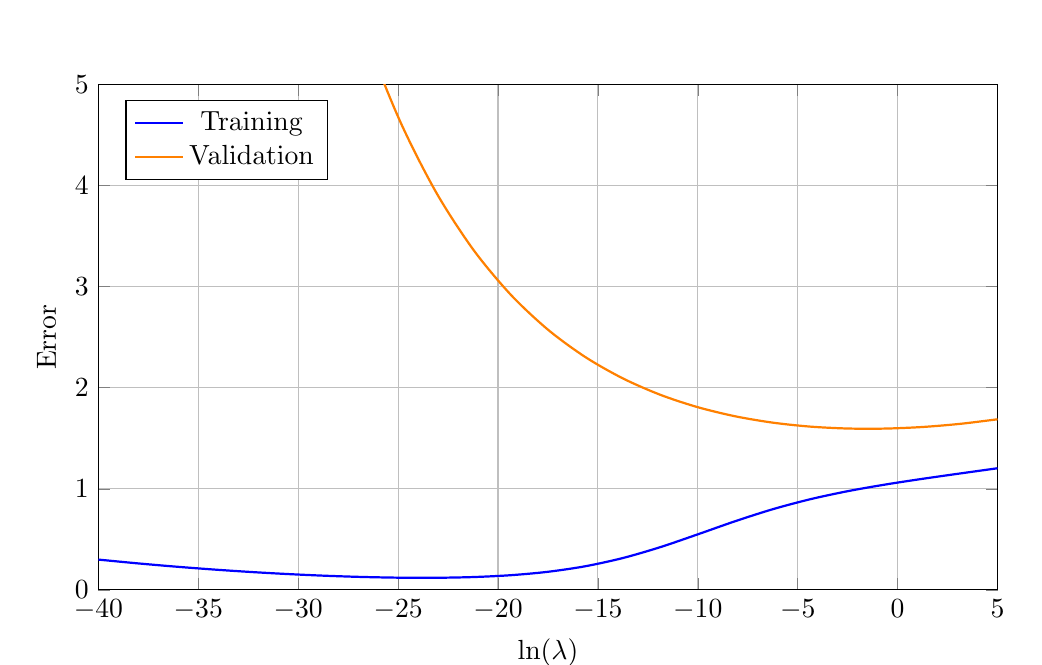
\begin{tikzpicture}
\begin{axis}[
    width=13cm,
    height=8cm,
    xlabel={$\ln(\lambda)$},
    ylabel={Error},
    xlabel style={font=\normalsize},
    ylabel style={font=\normalsize},
    xmin=-40, xmax=5,
    ymin=0, ymax=5,
    grid=major,
    legend pos=north west,
    legend style={font=\normalsize}
]

% Training error (blue, increasing)
\addplot[blue, thick, smooth, domain=-40:5] {0.1 + 0.05*(x+20)^2/100 + 0.8/(1+exp(-0.3*(x+10)))};
\addlegendentry{Training}

% Validation error (orange, U-shaped)
\addplot[orange, thick, smooth, domain=-40:5] {1.5 + 0.08*(x+5)^2/50 + 1.2*exp(-0.15*(x+20))};
\addlegendentry{Validation}


\end{axis}
\end{tikzpicture}
\caption{Training and Validation Error vs. $\ln(\lambda)$ (Regularization Strength)}
\end{figure}

\begin{itemize}
    \item \textbf{Left side (small $\lambda$)}: Low training error, high validation error $\rightarrow$ Overfitting
    \item \textbf{Middle region}: Both errors are low $\rightarrow$ Good fit
    \item \textbf{Right side (large $\lambda$)}: Both errors increase $\rightarrow$ Underfitting
\end{itemize}

The optimal $\lambda$ is found where the validation error is minimized.

\subsection{Generalization and Data Size}

An important theoretical result in machine learning relates training error to generalization error:

\begin{theorem}[Generalization with Infinite Data]
As the number of training samples approaches infinity, the training error approximates the generalization error:
\[
E(f; \mathcal{D}_n) \to E(f; p_{\text{data}}) \quad \text{as} \quad n \to \infty
\]
\end{theorem}

This means:
\begin{itemize}
    \item With a small dataset ($n = 15$), even a complex model ($M = 9$) may overfit because there isn't enough data to constrain the parameters
    \item With a large dataset ($n = 100$), the same complex model can generalize well because the abundant data prevents overfitting
    \item More data allows us to use more complex models without overfitting
\end{itemize}

\textbf{Visual example}:

\begin{figure}[h]
\centering
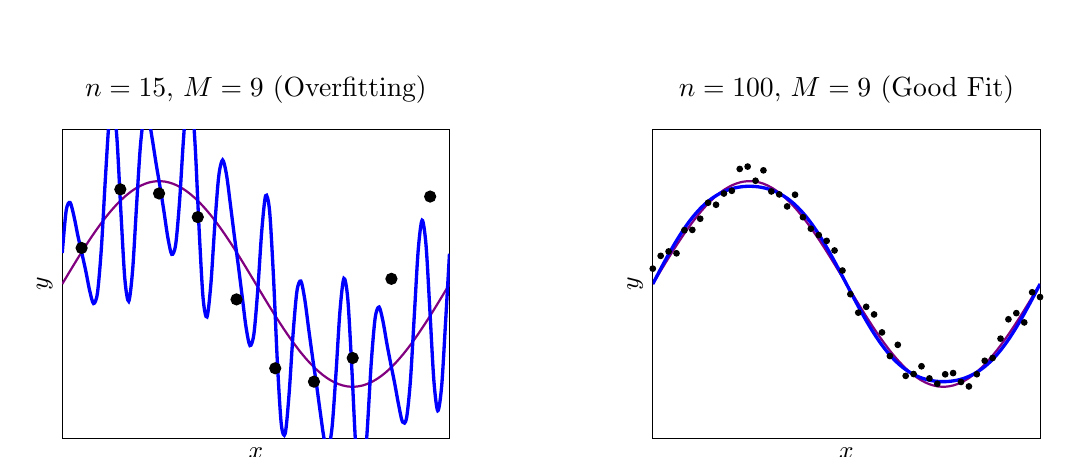
\begin{tikzpicture}

% n=15, M=9 (Overfitting)
\begin{scope}[xshift=0cm]
\begin{axis}[
    width=6.5cm,
    height=5.5cm,
    title={$n=15$, $M=9$ (Overfitting)},
    title style={font=\normalsize},
    xlabel={$x$},
    ylabel={$y$},
    xlabel style={font=\small},
    ylabel style={font=\small},
    xmin=0, xmax=1,
    ymin=-1.5, ymax=1.5,
    xtick=\empty,
    ytick=\empty,
]
% Few data points (15 points, but showing representative subset)
\addplot[only marks, mark=*, mark size=2pt, black] coordinates {
    (0.05, 0.35) (0.15, 0.92) (0.25, 0.88) (0.35, 0.65) (0.45, -0.15)
    (0.55, -0.82) (0.65, -0.95) (0.75, -0.72) (0.85, 0.05) (0.95, 0.85)
};
% True function (purple)
\addplot[violet, thick, smooth, domain=0:1, samples=50] {sin(deg(2*pi*x))};
% Overfitted polynomial (blue, oscillating wildly)
\addplot[blue, very thick, smooth, domain=0:1, samples=100] {
    sin(deg(2*pi*x)) + 0.8*sin(deg(20*pi*x)) + 0.3*cos(deg(30*pi*x))
};
\end{axis}
\end{scope}

% n=100, M=9 (Good fit)
\begin{scope}[xshift=7.5cm]
\begin{axis}[
    width=6.5cm,
    height=5.5cm,
    title={$n=100$, $M=9$ (Good Fit)},
    title style={font=\normalsize},
    xlabel={$x$},
    ylabel={$y$},
    xlabel style={font=\small},
    ylabel style={font=\small},
    xmin=0, xmax=1,
    ymin=-1.5, ymax=1.5,
    xtick=\empty,
    ytick=\empty,
]
% Many data points (showing more points)
\addplot[only marks, mark=*, mark size=1pt, black, samples=50, domain=0:1] {sin(deg(2*pi*x)) + 0.15*rand};
% True function (purple)
\addplot[violet, thick, smooth, domain=0:1, samples=50] {sin(deg(2*pi*x))};
% Well-fitted polynomial (blue, smooth)
\addplot[blue, very thick, smooth, domain=0:1, samples=100] {
    sin(deg(2*pi*x)) + 0.05*sin(deg(6*pi*x))
};
\end{axis}
\end{scope}

\end{tikzpicture}
\caption{Effect of data size on generalization: With few data points ($n=15$), a complex model ($M=9$) overfits. With many data points ($n=100$), the same model generalizes well. Purple: true function, Blue: fitted polynomial, Black dots: training data.}
\end{figure}

\begin{itemize}
    \item \textbf{$n = 15$, $M = 9$}: The 9th-degree polynomial overfits, oscillating wildly between the few training points
    \item \textbf{$n = 100$, $M = 9$}: With 100 training points, the same 9th-degree polynomial fits smoothly and generalizes well
\end{itemize}

\begin{center}
\colorbox{blue!10}{\parbox{0.9\textwidth}{
\centering
\textit{"Get more data" is often the most effective solution to overfitting}\\[0.1cm]
With sufficient data, even complex models can generalize well
}}
\end{center}



\newpage

\part{Model Evaluation and Regression Methods}

\section{Model Evaluation for Classification and Regression}

\subsection{Recap: Train, Validation, and Test Sets}

The machine learning workflow involves three distinct datasets, each serving a specific purpose:

\begin{figure}[h]
\centering
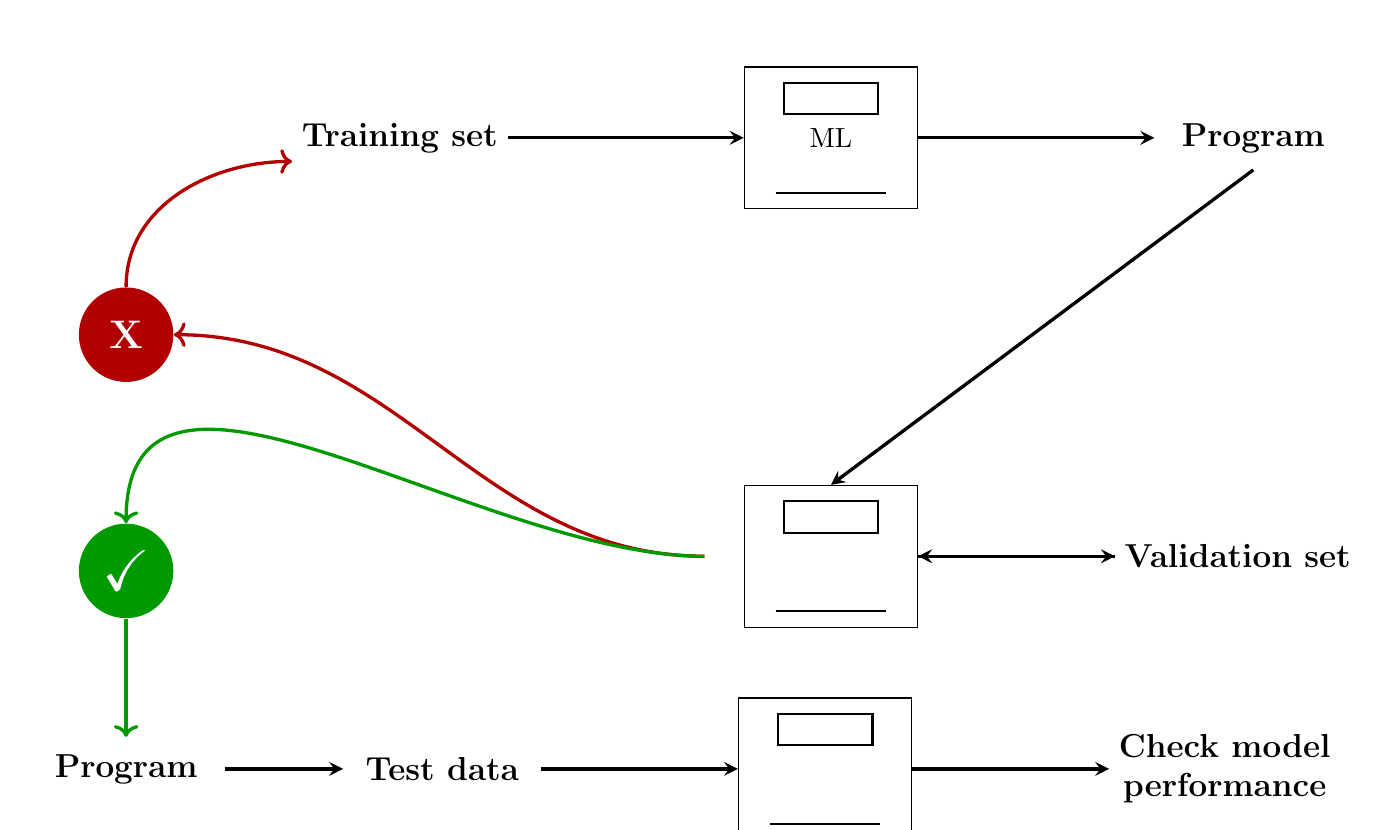
\begin{tikzpicture}[
    node distance=1.5cm and 2.5cm,
    box/.style={rectangle, minimum width=2.5cm, minimum height=0.8cm, align=center, font=\large\bfseries},
    computer/.style={rectangle, draw, minimum width=2.2cm, minimum height=1.8cm, align=center},
    arrow/.style={->, >=stealth, very thick}
]

% Top row: Training set -> ML Computer -> Program
\node[box] (train) {Training set};
\node[computer, right=3cm of train] (ml1) {ML};
\node[box, right=3cm of ml1] (program1) {Program};

% Draw computer screen
\draw[thick] ([xshift=-0.6cm, yshift=0.3cm]ml1.center) rectangle ([xshift=0.6cm, yshift=0.7cm]ml1.center);
\draw[thick] ([xshift=-0.7cm, yshift=-0.7cm]ml1.center) -- ([xshift=0.7cm, yshift=-0.7cm]ml1.center);

% Arrows for top row
\draw[arrow] (train) -- (ml1);
\draw[arrow] (ml1) -- (program1);

% Middle row: Validation evaluation with feedback
\node[computer, below=3.5cm of ml1] (ml2) {};
\node[box, right=2.5cm of ml2] (val) {Validation set};

% Draw computer screen for ml2
\draw[thick] ([xshift=-0.6cm, yshift=0.3cm]ml2.center) rectangle ([xshift=0.6cm, yshift=0.7cm]ml2.center);
\draw[thick] ([xshift=-0.7cm, yshift=-0.7cm]ml2.center) -- ([xshift=0.7cm, yshift=-0.7cm]ml2.center);

% Arrow from Program to validation computer
\draw[arrow] (program1.south) -- (ml2.north);

% Bidirectional arrows between validation computer and validation set
\draw[arrow] (ml2.east) -- (val.west);
\draw[arrow] (val.west) -- (ml2.east);

% Thumbs down (red) - feedback to training
\node[left=1.5cm of train, yshift=-2.5cm, fill=red!70!black, circle, minimum size=1.2cm] (thumbdown) {\textcolor{white}{\Large\textbf{X}}};
\draw[->, very thick, red!70!black] (thumbdown.north) to[out=90, in=180] ([yshift=-0.3cm]train.west);
\draw[->, very thick, red!70!black] ([xshift=-0.5cm]ml2.west) to[out=180, in=0] (thumbdown.east);

% Thumbs up (green) - proceed to testing
\node[left=1.5cm of train, yshift=-5.5cm, fill=green!60!black, circle, minimum size=1.2cm] (thumbup) {\textcolor{white}{\huge$\checkmark$}};
\node[box, below=1.5cm of thumbup] (program2) {Program};

\draw[->, very thick, green!60!black] (thumbup.south) -- (program2.north);
\draw[->, very thick, green!60!black] ([xshift=-0.5cm]ml2.west) to[out=180, in=90] (thumbup.north);

% Bottom row: Test data -> Computer -> Check model performance
\node[box, right=1.5cm of program2] (test) {Test data};
\node[computer, right=2.5cm of test] (ml3) {};
\node[box, right=2.5cm of ml3] (check) {Check model\\performance};

% Draw computer screen for ml3
\draw[thick] ([xshift=-0.6cm, yshift=0.3cm]ml3.center) rectangle ([xshift=0.6cm, yshift=0.7cm]ml3.center);
\draw[thick] ([xshift=-0.7cm, yshift=-0.7cm]ml3.center) -- ([xshift=0.7cm, yshift=-0.7cm]ml3.center);

% Arrows for bottom row
\draw[arrow] (program2) -- (test);
\draw[arrow] (test) -- (ml3);
\draw[arrow] (ml3) -- (check);

\end{tikzpicture}
\caption{Machine Learning Workflow: Training set trains the model, validation set evaluates and provides feedback (thumbs down = retrain, thumbs up = proceed to testing), test set checks final performance}
\end{figure}

\subsubsection{The Three Datasets}

\begin{enumerate}
    \item \textbf{Training Set}: Used to train the machine learning algorithm
    \begin{itemize}
        \item The model learns patterns and relationships from this data
        \item Parameters are optimized to minimize training error
    \end{itemize}
    
    \item \textbf{Validation Set}: Used during the learning phase
    \begin{itemize}
        \item Also called the \textit{mini test set}
        \item Helps select the better performing algorithm among alternatives
        \item Used to tune hyperparameters of the model
        \item Provides feedback to adjust the model before final testing
    \end{itemize}
    
    \item \textbf{Test Set}: Used for final model evaluation
    \begin{itemize}
        \item Provides an unbiased assessment of model performance
        \item The model has never seen this data during training or validation
        \item Tells us how well the model will perform on new, real-world data
    \end{itemize}
\end{enumerate}

\subsection{The Importance of the Validation Set}

The validation set plays a crucial role in the machine learning pipeline and must be kept \textbf{separate from the training set}.

\subsubsection{Why Separate the Validation Set?}

The validation set is used for two main purposes:

\begin{enumerate}
    \item \textbf{Algorithm Selection}: To pick the better performing algorithm
    \begin{itemize}
        \item Compare different model architectures (e.g., decision trees vs. neural networks)
        \item Select the model that performs best on unseen data
    \end{itemize}
    
    \item \textbf{Hyperparameter Tuning}: To decide the hyperparameters of an algorithm
    \begin{itemize}
        \item Hyperparameters are configuration settings that are not learned from data
        \item Examples: learning rate, regularization strength ($\lambda$), number of layers, tree depth
        \item The validation set helps find the optimal hyperparameter values
    \end{itemize}
\end{enumerate}

\begin{remark}
\textbf{ATTENTION}: Splitting the datasets into training and validation sets can be done randomly to avoid bias. However, there are some \textbf{specific rules} to apply when performing this split to ensure reliable model evaluation.
\end{remark}

\subsection{Specific Rules for Dataset Splitting}

When splitting data into training, validation, and testing sets, you can have conflicting priorities. The key is to balance these priorities appropriately.

\begin{figure}[h]
\centering
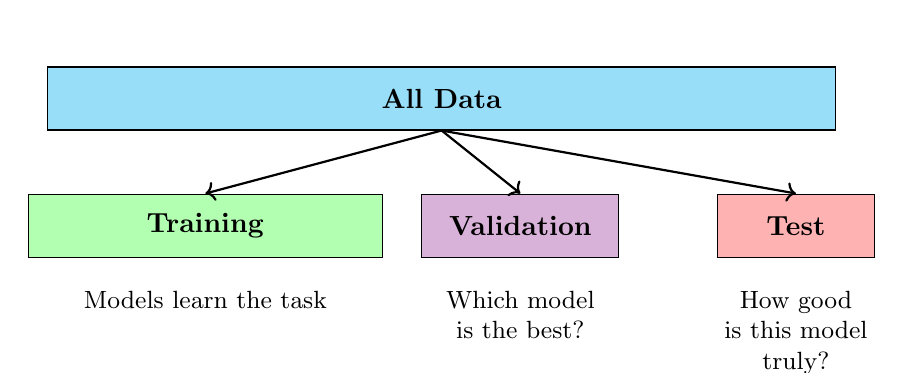
\begin{tikzpicture}[
    node distance=0.8cm,
    box/.style={rectangle, draw, minimum width=10cm, minimum height=0.8cm, align=center}
]

% All Data
\node[box, fill=cyan!40] (all) {\textbf{All Data}};

% Three splits
\node[box, fill=green!30, below=of all, xshift=-3cm, minimum width=4.5cm] (train) {\textbf{Training}};
\node[box, fill=violet!30, below=of all, xshift=1cm, minimum width=2.5cm] (val) {\textbf{Validation}};
\node[box, fill=red!30, below=of all, xshift=4.5cm, minimum width=2cm] (test) {\textbf{Test}};

% Descriptions
\node[below=0.3cm of train, align=center, font=\small] {Models learn the task};
\node[below=0.3cm of val, align=center, font=\small] {Which model\\is the best?};
\node[below=0.3cm of test, align=center, font=\small] {How good\\is this model\\truly?};

% Arrows
\draw[->, thick] (all.south) -- (train.north);
\draw[->, thick] (all.south) -- (val.north);
\draw[->, thick] (all.south) -- (test.north);

\end{tikzpicture}
\caption{Dataset splitting: Training for learning, Validation for model selection, Test for final evaluation}
\end{figure}

\subsubsection{Priority 1: Accurate Error Estimation}

\textbf{Goal}: Estimate future error (i.e., validation/testing error) as accurately as possible.

\textbf{How to achieve this}: By making the \textbf{validation set as big as possible}.

\textit{(High confidence interval)}

\begin{itemize}
    \item A larger validation set provides more reliable error estimates
    \item Reduces variance in performance metrics
    \item Gives higher confidence that the measured performance reflects true generalization
\end{itemize}

\subsubsection{Priority 2: Accurate Classifier Learning}

\textbf{Goal}: Learn classifier as accurately as possible.

\textbf{How to achieve this}: By making the \textbf{training set as big as possible}.

\textit{(Better estimates, maybe better generalization)}

\begin{itemize}
    \item More training data allows the model to learn more robust patterns
    \item Reduces overfitting by providing diverse examples
    \item Generally leads to better generalization on unseen data
\end{itemize}

\subsubsection{The Critical Rule}

\begin{center}
\colorbox{red!20}{\parbox{0.9\textwidth}{
\centering
\textbf{CRITICAL REQUIREMENT}\\[0.3cm]
Training and validation/testing instances \textbf{CANNOT OVERLAP !!!!}
}}
\end{center}

\begin{itemize}
    \item If the same data appears in both training and validation/test sets, the evaluation is invalid
    \item The model would be tested on data it has already seen during training
    \item This leads to overly optimistic performance estimates that don't reflect real-world performance
    \item Data leakage between sets is one of the most common mistakes in machine learning
\end{itemize}

\begin{observation}
The split between training and validation/test sets represents a fundamental tradeoff:
\begin{itemize}
    \item Larger training set $\rightarrow$ Better model learning, but less reliable error estimation
    \item Larger validation/test set $\rightarrow$ More reliable error estimation, but potentially worse model learning
\end{itemize}

Common splits include 70-15-15, 80-10-10, or 60-20-20 (train-validation-test), depending on the total dataset size and specific requirements.
\end{observation}

\section{Cross Validation}

\subsection{When Do We Need Cross Validation?}

In cases where we don't have enough data to randomly split between training (e.g., 60\% of the total data), validation (e.g., 20\% of the total data), and testing (e.g., 20\% of the total data), we need to use \textbf{cross-validation}.

\begin{definition}[Cross Validation]
Cross-validation is a resampling technique that involves reusing a portion of the training set itself to validate performance by retraining not just one, but $N$ models.
\end{definition}

\subsection{Key Characteristics of Cross Validation}

\begin{itemize}
    \item \textbf{Multiple models}: Cross-validation involves training $N$ models instead of just one
    
    \item \textbf{Computational cost}: Performing cross-validation requires $N$ training sessions and can be more computationally demanding
    
    \item \textbf{Better use of limited data}: When data is scarce, cross-validation allows us to use the available data more efficiently for both training and validation
\end{itemize}

\subsection{Fundamental Rules of Cross Validation}

Cross validation must respect certain constraints to ensure valid model evaluation:

\begin{enumerate}
    \item \textbf{No overlap}: Training and validation cannot overlap, but $n_{\text{train}} + n_{\text{validation}} = \text{constant}$
    
    \item \textbf{Each instance used once per fold}: At each fold (step), you use each instance only in one set, so there is no overlapping within a single fold
    
    \item \textbf{Every sample participates}: Every sample is in both training and testing but not at the same time
    \begin{itemize}
        \item This reduces the chances of getting a biased training set
        \item Ensures all data contributes to both training and validation across different folds
    \end{itemize}
\end{enumerate}

\subsection{K-Fold Cross Validation}

K-fold cross validation is the most common form of cross validation, where the dataset is divided into $k$ equal parts (folds).

\subsubsection{How K-Fold Cross Validation Works}

In the case of k-fold cross-validation:

\begin{enumerate}
    \item We split our dataset into $k$ groups (folds)
    
    \item We perform training $k$ times on $(N/k)(k-1)$ data points
    
    \item We measure performance on the last $N/k$ data points (the validation fold)
    
    \item Our cross-validation performance will be the \textbf{average of the performance of the $k$ tests}
\end{enumerate}

\begin{remark}
\textbf{Important constraint}: Training set and validation set cannot overlap, but the sum of training and validation data is a constant (the total dataset size).
\end{remark}

\subsubsection{Visual Representation of K-Fold Cross Validation}

\begin{figure}[h]
\centering
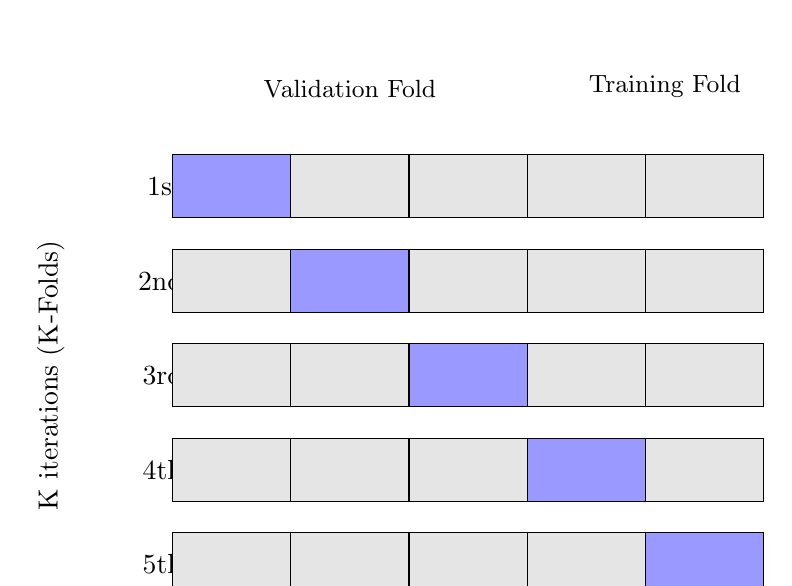
\begin{tikzpicture}[
    fold/.style={rectangle, draw, minimum width=1.5cm, minimum height=0.8cm},
    val/.style={fill=blue!40},
    train/.style={fill=gray!20}
]

% Labels
\node[anchor=east] at (-0.5, 0) {1st};
\node[anchor=east] at (-0.5, -1.2) {2nd};
\node[anchor=east] at (-0.5, -2.4) {3rd};
\node[anchor=east] at (-0.5, -3.6) {4th};
\node[anchor=east] at (-0.5, -4.8) {5th};

\node[anchor=south, font=\small] at (1.5, 1) {Validation Fold};
\node[anchor=south, font=\small] at (5.5, 1) {Training Fold};

% Fold 1
\node[fold, val] at (0, 0) {};
\node[fold, train] at (1.5, 0) {};
\node[fold, train] at (3, 0) {};
\node[fold, train] at (4.5, 0) {};
\node[fold, train] at (6, 0) {};

% Fold 2
\node[fold, train] at (0, -1.2) {};
\node[fold, val] at (1.5, -1.2) {};
\node[fold, train] at (3, -1.2) {};
\node[fold, train] at (4.5, -1.2) {};
\node[fold, train] at (6, -1.2) {};

% Fold 3
\node[fold, train] at (0, -2.4) {};
\node[fold, train] at (1.5, -2.4) {};
\node[fold, val] at (3, -2.4) {};
\node[fold, train] at (4.5, -2.4) {};
\node[fold, train] at (6, -2.4) {};

% Fold 4
\node[fold, train] at (0, -3.6) {};
\node[fold, train] at (1.5, -3.6) {};
\node[fold, train] at (3, -3.6) {};
\node[fold, val] at (4.5, -3.6) {};
\node[fold, train] at (6, -3.6) {};

% Fold 5
\node[fold, train] at (0, -4.8) {};
\node[fold, train] at (1.5, -4.8) {};
\node[fold, train] at (3, -4.8) {};
\node[fold, train] at (4.5, -4.8) {};
\node[fold, val] at (6, -4.8) {};

% Y-axis label
\node[rotate=90, anchor=south] at (-2, -2.4) {K iterations (K-Folds)};

\end{tikzpicture}
\caption{K-Fold Cross Validation: Each row represents one iteration where a different fold serves as validation (blue) while the rest serve as training (gray)}
\end{figure}

\subsection{Example: 5-Fold Cross Validation}

Let's examine a concrete example with 5 folds:

\begin{itemize}
    \item \textbf{Step 1}: Randomly split the data into 5 folds
    \item \textbf{Step 2}: Test on each fold while training on 4 other folds (80\% train, 20\% test)
    \item \textbf{Step 3}: Average the results over 5 folds
\end{itemize}

\begin{figure}[h]
\centering
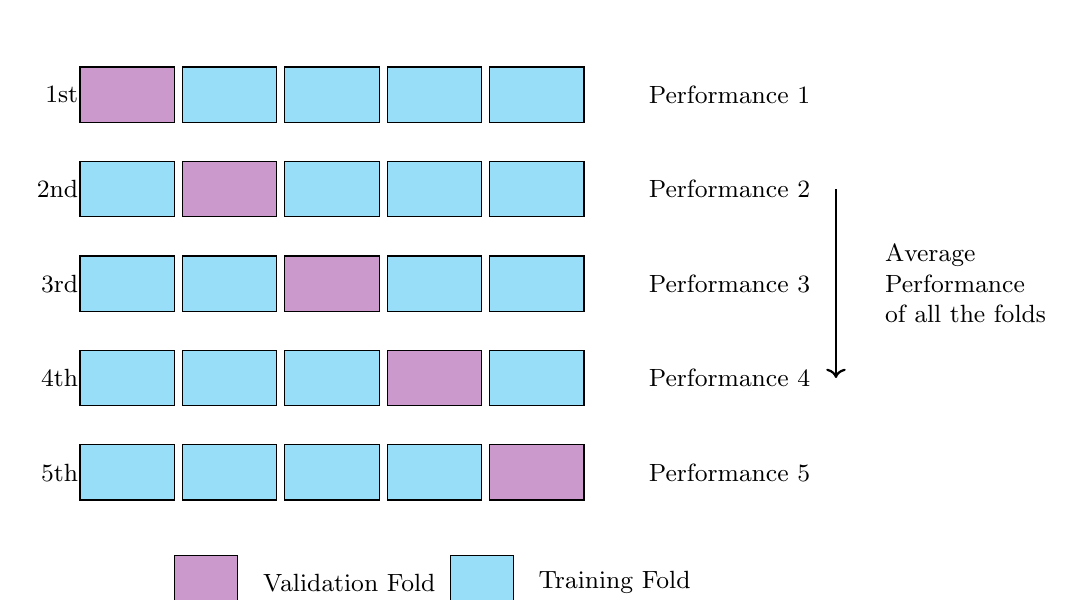
\begin{tikzpicture}[
    fold/.style={rectangle, draw, minimum width=1.2cm, minimum height=0.7cm},
    val/.style={fill=violet!40},
    train/.style={fill=cyan!40}
]

% Iteration labels
\node[anchor=east, font=\small] at (-0.5, 0) {1st};
\node[anchor=east, font=\small] at (-0.5, -1.2) {2nd};
\node[anchor=east, font=\small] at (-0.5, -2.4) {3rd};
\node[anchor=east, font=\small] at (-0.5, -3.6) {4th};
\node[anchor=east, font=\small] at (-0.5, -4.8) {5th};

% Fold 1
\node[fold, val] at (0, 0) {};
\node[fold, train] at (1.3, 0) {};
\node[fold, train] at (2.6, 0) {};
\node[fold, train] at (3.9, 0) {};
\node[fold, train] at (5.2, 0) {};
\node[anchor=west, font=\small] at (6.5, 0) {Performance 1};

% Fold 2
\node[fold, train] at (0, -1.2) {};
\node[fold, val] at (1.3, -1.2) {};
\node[fold, train] at (2.6, -1.2) {};
\node[fold, train] at (3.9, -1.2) {};
\node[fold, train] at (5.2, -1.2) {};
\node[anchor=west, font=\small] at (6.5, -1.2) {Performance 2};

% Fold 3
\node[fold, train] at (0, -2.4) {};
\node[fold, train] at (1.3, -2.4) {};
\node[fold, val] at (2.6, -2.4) {};
\node[fold, train] at (3.9, -2.4) {};
\node[fold, train] at (5.2, -2.4) {};
\node[anchor=west, font=\small] at (6.5, -2.4) {Performance 3};

% Fold 4
\node[fold, train] at (0, -3.6) {};
\node[fold, train] at (1.3, -3.6) {};
\node[fold, train] at (2.6, -3.6) {};
\node[fold, val] at (3.9, -3.6) {};
\node[fold, train] at (5.2, -3.6) {};
\node[anchor=west, font=\small] at (6.5, -3.6) {Performance 4};

% Fold 5
\node[fold, train] at (0, -4.8) {};
\node[fold, train] at (1.3, -4.8) {};
\node[fold, train] at (2.6, -4.8) {};
\node[fold, train] at (3.9, -4.8) {};
\node[fold, val] at (5.2, -4.8) {};
\node[anchor=west, font=\small] at (6.5, -4.8) {Performance 5};

% Arrow and final result
\draw[->, thick] (9, -1.2) -- (9, -3.6);
\node[anchor=west, font=\small, align=left] at (9.5, -2.4) {Average\\Performance\\of all the folds};

% Legend
\node[fold, val, minimum width=0.8cm] at (1, -6.2) {};
\node[anchor=west, font=\small] at (1.6, -6.2) {Validation Fold};
\node[fold, train, minimum width=0.8cm] at (4.5, -6.2) {};
\node[anchor=west, font=\small] at (5.1, -6.2) {Training Fold};

\end{tikzpicture}
\caption{5-Fold Cross Validation Example: Each fold serves as validation once, and the final performance is the average of all 5 iterations}
\end{figure}

\subsubsection{The Process in Detail}

For each of the 5 iterations:

\begin{enumerate}
    \item \textbf{Iteration 1}: Use fold 1 as validation, folds 2-5 as training $\rightarrow$ Get Performance 1
    \item \textbf{Iteration 2}: Use fold 2 as validation, folds 1,3-5 as training $\rightarrow$ Get Performance 2
    \item \textbf{Iteration 3}: Use fold 3 as validation, folds 1-2,4-5 as training $\rightarrow$ Get Performance 3
    \item \textbf{Iteration 4}: Use fold 4 as validation, folds 1-3,5 as training $\rightarrow$ Get Performance 4
    \item \textbf{Iteration 5}: Use fold 5 as validation, folds 1-4 as training $\rightarrow$ Get Performance 5
\end{enumerate}

\textbf{Final Cross-Validation Performance}:
\[
\text{CV Performance} = \frac{1}{5} \sum_{i=1}^{5} \text{Performance}_i
\]

\subsection{Advantages of Cross Validation}

\begin{itemize}
    \item \textbf{Better use of limited data}: Every data point is used for both training and validation
    
    \item \textbf{More reliable performance estimates}: Averaging over multiple folds reduces variance in the performance estimate
    
    \item \textbf{Reduces bias}: Every sample participates in validation, reducing the risk of a biased validation set
    
    \item \textbf{Detects overfitting}: If performance varies significantly across folds, it may indicate overfitting or data quality issues
\end{itemize}

\subsection{Disadvantages of Cross Validation}

\begin{itemize}
    \item \textbf{Computationally expensive}: Requires training $k$ models instead of one
    
    \item \textbf{Time-consuming}: Training time is multiplied by the number of folds
    
    \item \textbf{Not suitable for very large datasets}: When data is abundant, a simple train-validation-test split is more efficient
\end{itemize}

\begin{observation}
The choice of $k$ (number of folds) involves a tradeoff:
\begin{itemize}
    \item \textbf{Larger $k$}: More accurate performance estimate, but more computationally expensive
    \item \textbf{Smaller $k$}: Faster computation, but less reliable performance estimate
    \item Common choices: $k = 5$ or $k = 10$
    \item Extreme case: $k = N$ (Leave-One-Out Cross Validation) uses each single sample as validation once
\end{itemize}
\end{observation}

\section{Leave-One-Out Cross Validation}

\subsection{What is Leave-One-Out Cross Validation?}

Leave-One-Out Cross Validation (LOOCV) is an extreme case of k-fold cross validation that is particularly useful when we have very few data points.

\begin{definition}[Leave-One-Out Cross Validation]
LOOCV is $n$-fold cross validation where $n$ equals the total number of samples. In each iteration, we train on all $(n-1)$ samples and test on exactly 1 instance.
\end{definition}

\subsection{How LOOCV Works}

The process involves:

\begin{enumerate}
    \item Take the entire dataset of $n$ samples
    \item For each sample $i$ (where $i = 1, 2, \ldots, n$):
    \begin{itemize}
        \item Use sample $i$ as the validation set (1 sample)
        \item Use all other samples $(n-1)$ as the training set
        \item Train the model and evaluate on the single validation sample
    \end{itemize}
    \item Repeat this process $n$ times (once for each sample)
    \item Average the performance across all $n$ experiments
\end{enumerate}

\begin{figure}[h]
\centering
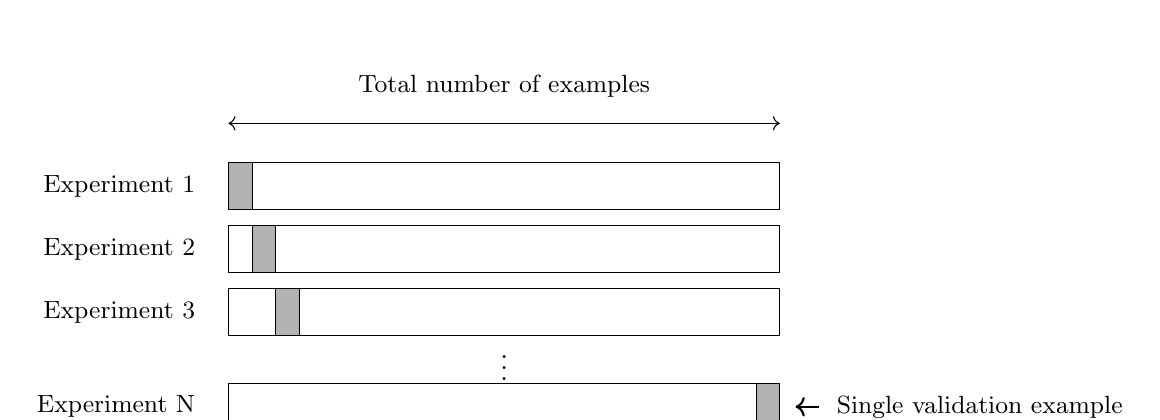
\begin{tikzpicture}[
    box/.style={rectangle, draw, minimum width=7cm, minimum height=0.6cm},
    val/.style={fill=gray!60},
    train/.style={fill=white}
]

% Title
\node[anchor=south] at (3.5, 3.5) {\small Total number of examples};
\draw[<->] (0, 3.3) -- (7, 3.3);

% Experiment 1
\node[anchor=east, font=\small] at (-0.3, 2.5) {Experiment 1};
\node[box, train] at (3.5, 2.5) {};
\node[rectangle, draw, fill=gray!60, minimum width=0.3cm, minimum height=0.6cm] at (0.15, 2.5) {};

% Experiment 2
\node[anchor=east, font=\small] at (-0.3, 1.7) {Experiment 2};
\node[box, train] at (3.5, 1.7) {};
\node[rectangle, draw, fill=gray!60, minimum width=0.3cm, minimum height=0.6cm] at (0.45, 1.7) {};

% Experiment 3
\node[anchor=east, font=\small] at (-0.3, 0.9) {Experiment 3};
\node[box, train] at (3.5, 0.9) {};
\node[rectangle, draw, fill=gray!60, minimum width=0.3cm, minimum height=0.6cm] at (0.75, 0.9) {};

% Dots
\node at (3.5, 0.3) {$\vdots$};

% Experiment N
\node[anchor=east, font=\small] at (-0.3, -0.3) {Experiment N};
\node[box, train] at (3.5, -0.3) {};
\node[rectangle, draw, fill=gray!60, minimum width=0.3cm, minimum height=0.6cm] at (6.85, -0.3) {};

% Arrow pointing to validation
\draw[->, thick] (7.5, -0.3) -- (7.2, -0.3);
\node[anchor=west, font=\small] at (7.6, -0.3) {Single validation example};

\end{tikzpicture}
\caption{Leave-One-Out Cross Validation: Each experiment uses exactly one sample for validation (gray) and all others for training (white)}
\end{figure}

\subsection{Pros and Cons of LOOCV}

\subsubsection{Advantages}

\begin{itemize}
    \item \textbf{Best possible classifier}: The model is learned from $n-1$ training examples, which is the maximum possible training data
    
    \item \textbf{Maximizes training data}: Each model uses almost all available data for training
    
    \item \textbf{Unbiased estimate}: Provides a nearly unbiased estimate of model performance
    
    \item \textbf{Deterministic}: No randomness in the splitting process (every sample is used exactly once as validation)
\end{itemize}

\subsubsection{Disadvantages}

\begin{itemize}
    \item \textbf{High computational cost}: Must re-learn everything for $n$ times, where $n$ is the total number of samples
    
    \item \textbf{Time-consuming}: For large datasets, LOOCV becomes impractical
    
    \item \textbf{High variance}: Performance estimates can have high variance, especially with small datasets
\end{itemize}

\begin{remark}
LOOCV is most appropriate when:
\begin{itemize}
    \item The dataset is very small (e.g., $n < 50$)
    \item Computational resources are available
    \item You need the most accurate performance estimate possible
\end{itemize}

For larger datasets, standard k-fold cross validation (with $k = 5$ or $k = 10$) is typically preferred due to its better balance between computational cost and performance estimation accuracy.
\end{remark}

\section{Stratification in Cross Validation}

\subsection{The Problem: Imbalanced Classes}

In many real-world datasets, class labels are not evenly distributed. For example, in a medical diagnosis dataset, healthy patients might vastly outnumber sick patients. When performing cross validation on such imbalanced datasets, random splitting can lead to folds with very different class distributions.

\subsection{What is Stratification?}

\begin{definition}[Stratification]
Stratification is a technique to keep class labels \textbf{balanced across training and validation sets} during cross validation. Instead of randomly dividing the dataset, we ensure that each fold maintains approximately the same proportion of samples for each class as the complete dataset.
\end{definition}

\subsection{How Stratified K-Fold Works}

The stratification process works as follows:

\begin{enumerate}
    \item \textbf{Divide by class}: Instead of taking the dataset and dividing it randomly into $K$ parts, take the dataset and divide it into individual classes
    
    \item \textbf{Split each class}: Then for each class, divide the instances into $K$ parts
    
    \item \textbf{Assemble folds}: Assemble the $i$-th part from all classes to make the $i$-th fold
    
    \item \textbf{Important}: It is still random! The splitting within each class is random, but the proportions are maintained
\end{enumerate}

\begin{figure}[h]
\centering
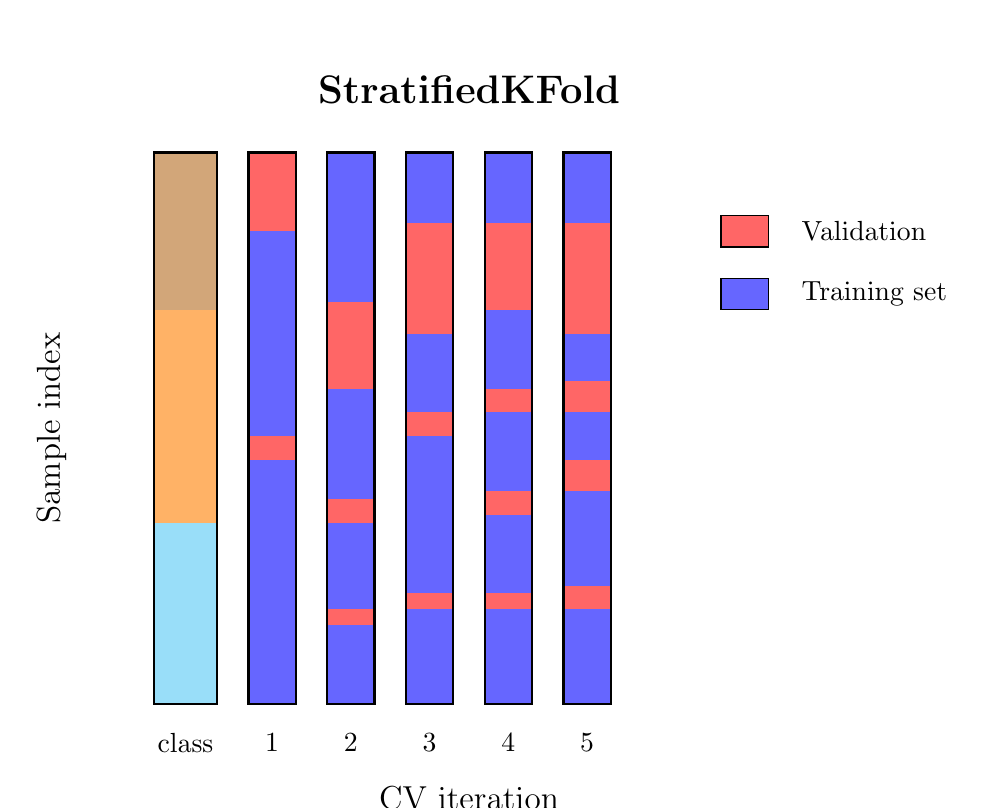
\begin{tikzpicture}

% Title
\node[font=\Large\bfseries] at (4, 7.8) {StratifiedKFold};

% Y-axis label
\node[rotate=90, font=\large] at (-1.3, 3.5) {Sample index};

% X-axis label
\node[font=\large] at (4, -1.2) {CV iteration};

% Column labels
\node[font=\normalsize] at (0.4, -0.5) {class};
\node[font=\normalsize] at (1.5, -0.5) {1};
\node[font=\normalsize] at (2.5, -0.5) {2};
\node[font=\normalsize] at (3.5, -0.5) {3};
\node[font=\normalsize] at (4.5, -0.5) {4};
\node[font=\normalsize] at (5.5, -0.5) {5};

% Class column (first column) - 3 colors
\fill[cyan!40] (0, 0) rectangle (0.8, 2.3);
\fill[orange!60] (0, 2.3) rectangle (0.8, 5);
\fill[brown!70] (0, 5) rectangle (0.8, 7);

% Fold 1
\fill[blue!60] (1.2, 0) rectangle (1.8, 3.1);
\fill[red!60] (1.2, 3.1) rectangle (1.8, 3.4);
\fill[blue!60] (1.2, 3.4) rectangle (1.8, 6);
\fill[red!60] (1.2, 6) rectangle (1.8, 7);

% Fold 2
\fill[blue!60] (2.2, 0) rectangle (2.8, 1);
\fill[red!60] (2.2, 1) rectangle (2.8, 1.2);
\fill[blue!60] (2.2, 1.2) rectangle (2.8, 2.3);
\fill[red!60] (2.2, 2.3) rectangle (2.8, 2.6);
\fill[blue!60] (2.2, 2.6) rectangle (2.8, 4);
\fill[red!60] (2.2, 4) rectangle (2.8, 5.1);
\fill[blue!60] (2.2, 5.1) rectangle (2.8, 7);

% Fold 3
\fill[blue!60] (3.2, 0) rectangle (3.8, 1.2);
\fill[red!60] (3.2, 1.2) rectangle (3.8, 1.4);
\fill[blue!60] (3.2, 1.4) rectangle (3.8, 3.4);
\fill[red!60] (3.2, 3.4) rectangle (3.8, 3.7);
\fill[blue!60] (3.2, 3.7) rectangle (3.8, 4.7);
\fill[red!60] (3.2, 4.7) rectangle (3.8, 6.1);
\fill[blue!60] (3.2, 6.1) rectangle (3.8, 7);

% Fold 4
\fill[blue!60] (4.2, 0) rectangle (4.8, 1.2);
\fill[red!60] (4.2, 1.2) rectangle (4.8, 1.4);
\fill[blue!60] (4.2, 1.4) rectangle (4.8, 2.4);
\fill[red!60] (4.2, 2.4) rectangle (4.8, 2.7);
\fill[blue!60] (4.2, 2.7) rectangle (4.8, 3.7);
\fill[red!60] (4.2, 3.7) rectangle (4.8, 4);
\fill[blue!60] (4.2, 4) rectangle (4.8, 5);
\fill[red!60] (4.2, 5) rectangle (4.8, 6.1);
\fill[blue!60] (4.2, 6.1) rectangle (4.8, 7);

% Fold 5
\fill[blue!60] (5.2, 0) rectangle (5.8, 1.2);
\fill[red!60] (5.2, 1.2) rectangle (5.8, 1.5);
\fill[blue!60] (5.2, 1.5) rectangle (5.8, 2.7);
\fill[red!60] (5.2, 2.7) rectangle (5.8, 3.1);
\fill[blue!60] (5.2, 3.1) rectangle (5.8, 3.7);
\fill[red!60] (5.2, 3.7) rectangle (5.8, 4.1);
\fill[blue!60] (5.2, 4.1) rectangle (5.8, 4.7);
\fill[red!60] (5.2, 4.7) rectangle (5.8, 6.1);
\fill[blue!60] (5.2, 6.1) rectangle (5.8, 7);

% Draw borders for all columns
\draw[thick] (0, 0) rectangle (0.8, 7);
\draw[thick] (1.2, 0) rectangle (1.8, 7);
\draw[thick] (2.2, 0) rectangle (2.8, 7);
\draw[thick] (3.2, 0) rectangle (3.8, 7);
\draw[thick] (4.2, 0) rectangle (4.8, 7);
\draw[thick] (5.2, 0) rectangle (5.8, 7);

% Legend
\node[rectangle, fill=red!60, draw, minimum width=0.6cm, minimum height=0.4cm] at (7.5, 6) {};
\node[anchor=west, font=\normalsize] at (8.1, 6) {Validation};

\node[rectangle, fill=blue!60, draw, minimum width=0.6cm, minimum height=0.4cm] at (7.5, 5.2) {};
\node[anchor=west, font=\normalsize] at (8.1, 5.2) {Training set};

\end{tikzpicture}
\caption{Stratified K-Fold: Each fold maintains the same class proportions across all folds}
\end{figure}

\subsection{Example: Stratified 5-Fold Cross Validation}

Let's consider a concrete scenario with an imbalanced dataset containing 300 samples, divided into three classes (A, B, and C), where Class A has more samples than the other two.

\subsubsection{Imbalanced Dataset}

\begin{itemize}
    \item \textbf{Class A}: 200 samples (66.7\%)
    \item \textbf{Class B}: 50 samples (16.7\%)
    \item \textbf{Class C}: 50 samples (16.7\%)
    \item \textbf{Total}: 300 samples
\end{itemize}

\subsubsection{Split the Dataset into Five Folds with Stratification}

Each fold will have 60 samples total, maintaining the class proportions:

\begin{itemize}
    \item \textbf{Fold 1}: 60 samples (Class A: 40, Class B: 10, Class C: 10)
    \item \textbf{Fold 2}: 60 samples (Class A: 40, Class B: 10, Class C: 10)
    \item \textbf{Fold 3}: 60 samples (Class A: 40, Class B: 10, Class C: 10)
    \item \textbf{Fold 4}: 60 samples (Class A: 40, Class B: 10, Class C: 10)
    \item \textbf{Fold 5}: 60 samples (Class A: 40, Class B: 10, Class C: 10)
\end{itemize}

Notice that each fold maintains the same 66.7\%-16.7\%-16.7\% class distribution as the original dataset.

\subsubsection{Train and Validate}

The cross-validation process proceeds as follows:

\begin{enumerate}
    \item \textbf{Iteration 1}: Train on Folds 1, 2, 3, and 4, Validate on Fold 5
    \item \textbf{Iteration 2}: Train on Folds 2, 3, 4, and 5, Validate on Fold 1
    \item \textbf{Iteration 3}: Train on Folds 1, 3, 4, and 5, Validate on Fold 2
    \item \textbf{Iteration 4}: Train on Folds 1, 2, 4, and 5, Validate on Fold 3
    \item \textbf{Iteration 5}: Train on Folds 1, 2, 3, and 5, Validate on Fold 4
\end{enumerate}

\subsubsection{Average the Performance Metrics}

\begin{itemize}
    \item Calculate performance metrics for each iteration
    \item Average these metrics to evaluate the model's performance robustly
\end{itemize}

\subsection{Why Stratification Matters}

\begin{itemize}
    \item \textbf{Prevents biased folds}: Without stratification, some folds might have very few (or no) examples of minority classes
    
    \item \textbf{Consistent evaluation}: Each fold represents the overall dataset distribution, leading to more reliable performance estimates
    
    \item \textbf{Better for imbalanced datasets}: Particularly important when dealing with class imbalance
    
    \item \textbf{Reduces variance}: Performance estimates have lower variance across folds
\end{itemize}

\begin{remark}
\textbf{When to use stratification}:
\begin{itemize}
    \item Always use stratification for classification problems with imbalanced classes
    \item It's generally a good practice even for balanced datasets
    \item Most machine learning libraries (e.g., scikit-learn) provide stratified cross-validation functions
    \item For regression problems, stratification is not applicable (since there are no discrete classes)
\end{itemize}
\end{remark}

\begin{observation}
Stratification ensures that:
\begin{itemize}
    \item Each fold is a good representative of the whole dataset
    \item Minority classes are adequately represented in both training and validation sets
    \item Performance metrics are more stable and reliable across folds
    \item The model sees a balanced distribution of classes during each training iteration
\end{itemize}
\end{observation}

\section{Evaluation Measures}

Once we have trained our models and performed cross-validation, we need to evaluate their performance. Different tasks require different evaluation metrics.

\subsection{Why Do We Need Evaluation Measures?}

Evaluation measures serve two primary purposes:

\begin{enumerate}
    \item \textbf{To decide if our model is performing well}: Assess whether the model meets the requirements for the task
    
    \item \textbf{To decide out of many models, which one performs better than the other}: Compare different models and select the best one for deployment
\end{enumerate}

\subsection{Evaluation Measures by Task Type}

Different machine learning tasks require different evaluation approaches:

\subsubsection{Classification}

\textbf{Question}: How often does our model classify something right/wrong?

Classification metrics measure the correctness of predictions, focusing on whether the predicted class matches the actual class.

\subsubsection{Regression}

\textbf{Question}: How close is our model to what we are trying to predict?

Regression metrics measure the distance or error between predicted continuous values and actual values.

\subsubsection{Clustering}

\textbf{Question}: How well does our model describe our data?

Clustering evaluation is generally very hard because there's often no ground truth to compare against. Metrics must assess the quality of discovered patterns.

\section{Evaluation Measures for Classification}

\subsection{Types of Classification Problems}

A classification model takes a set of features as input and produces one or more classes as output.

\begin{definition}[Classification Types]
Classification can be categorized into different types based on the number of classes:

\begin{itemize}
    \item \textbf{Binary Classification}: In the case of two classes (0/1) or one vs rest (e.g., apples vs other fruits)
    
    \item \textbf{Multi-class Classification}: In the case of having $N$ classes to choose from (e.g., cat, dog, wolf, etc.)
    
    \item \textbf{Multi-label Classification}: A problem where an example can belong to multiple classes simultaneously
\end{itemize}
\end{definition}

\subsection{The Confusion Matrix}

The confusion matrix is a fundamental tool for evaluating binary classification models. It provides a complete picture of how the model performs across different types of predictions.

\subsubsection{Confusion Matrix for Binary Classification}

\begin{figure}[h]
\centering
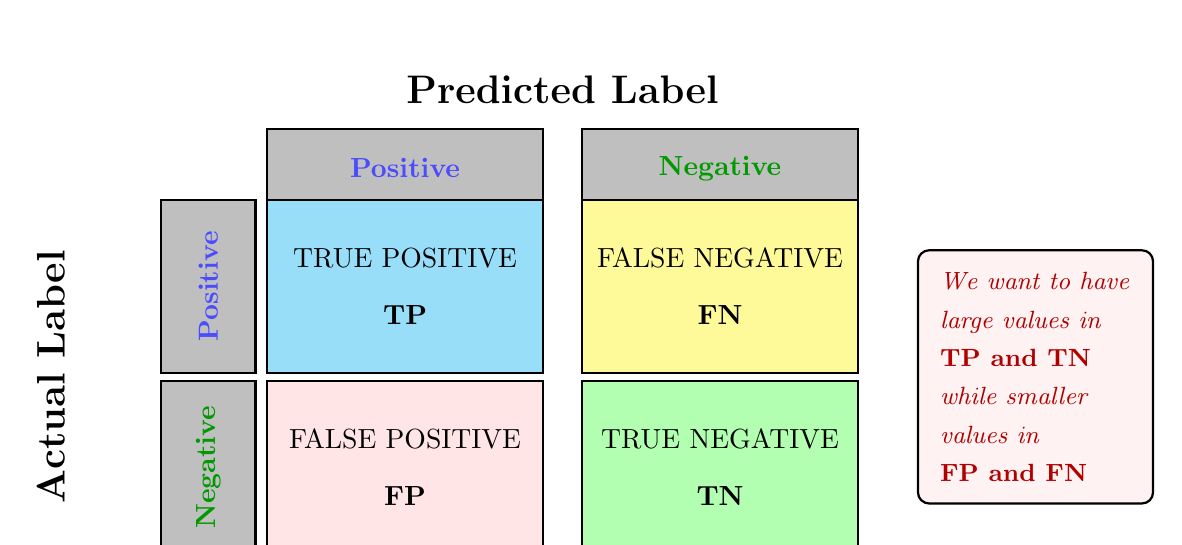
\begin{tikzpicture}[
    cell/.style={rectangle, draw, thick, minimum width=3.5cm, minimum height=2.2cm, align=center, font=\normalsize},
    header/.style={rectangle, draw, thick, fill=gray!50, align=center, font=\bfseries}
]

% Top header - Predicted Label
\node[font=\Large\bfseries] at (4, 4.5) {Predicted Label};

% Column headers (horizontal text)
\node[header, minimum width=3.5cm, minimum height=1cm] at (2, 3.5) {\textcolor{blue!70}{Positive}};
\node[header, minimum width=3.5cm, minimum height=1cm] at (6, 3.5) {\textcolor{green!60!black}{Negative}};

% Left header - Actual Label
\node[font=\Large\bfseries, rotate=90] at (-2.5, 0.85) {Actual Label};

% Row headers (vertical text)
\node[header, minimum width=2.2cm, minimum height=1.2cm, rotate=90] at (-0.5, 2) {\textcolor{blue!70}{Positive}};
\node[header, minimum width=2.2cm, minimum height=1.2cm, rotate=90] at (-0.5, -0.3) {\textcolor{green!60!black}{Negative}};

% Matrix cells (all same size)
\node[cell, fill=cyan!40] at (2, 2) {TRUE POSITIVE\\[0.3cm]\textbf{TP}};
\node[cell, fill=yellow!40] at (6, 2) {FALSE NEGATIVE\\[0.3cm]\textbf{FN}};
\node[cell, fill=pink!40] at (2, -0.3) {FALSE POSITIVE\\[0.3cm]\textbf{FP}};
\node[cell, fill=green!30] at (6, -0.3) {TRUE NEGATIVE\\[0.3cm]\textbf{TN}};

% Note box
\node[anchor=west, align=left, font=\small, text=red!70!black, draw, thick, rounded corners, fill=red!5, inner sep=8pt] at (8.5, 0.85) {
    \textit{We want to have}\\[0.1cm]
    \textit{large values in}\\[0.1cm]
    \textbf{TP and TN}\\[0.1cm]
    \textit{while smaller}\\[0.1cm]
    \textit{values in}\\[0.1cm]
    \textbf{FP and FN}
};

\end{tikzpicture}
\caption{Confusion Matrix for Binary Classification}
\end{figure}

\subsubsection{Understanding the Confusion Matrix}

The confusion matrix has four components:

\begin{itemize}
    \item \textbf{True Positive (TP)}: The model correctly predicted the positive class
    \begin{itemize}
        \item Actual label: Positive
        \item Predicted label: Positive
        \item \textcolor{blue!70}{Good prediction!}
    \end{itemize}
    
    \item \textbf{True Negative (TN)}: The model correctly predicted the negative class
    \begin{itemize}
        \item Actual label: Negative
        \item Predicted label: Negative
        \item \textcolor{green!60!black}{Good prediction!}
    \end{itemize}
    
    \item \textbf{False Positive (FP)}: The model incorrectly predicted positive (Type I error)
    \begin{itemize}
        \item Actual label: Negative
        \item Predicted label: Positive
        \item \textcolor{red}{Bad prediction!} (False alarm)
    \end{itemize}
    
    \item \textbf{False Negative (FN)}: The model incorrectly predicted negative (Type II error)
    \begin{itemize}
        \item Actual label: Positive
        \item Predicted label: Negative
        \item \textcolor{red}{Bad prediction!} (Missed detection)
    \end{itemize}
\end{itemize}

\begin{remark}
\textbf{Goal}: We want to maximize TP and TN (correct predictions) while minimizing FP and FN (incorrect predictions).
\end{remark}

\subsection{Classification Error and Accuracy}

From the confusion matrix, we can derive several important metrics.

\subsubsection{Classification Error}

\begin{definition}[Classification Error]
The classification error (also called misclassification rate) measures the proportion of incorrect predictions:

\[
\text{Classification Error} = \frac{FP + FN}{TP + TN + FP + FN}
\]

This represents the fraction of all predictions that were wrong.
\end{definition}

\subsubsection{Accuracy}

\begin{definition}[Accuracy]
Accuracy measures the proportion of correct predictions:

\[
\text{Accuracy} = 1 - \text{Error} = \frac{TP + TN}{TP + TN + FP + FN}
\]

This represents the fraction of all predictions that were correct.
\end{definition}

\subsection{The Problem with Accuracy: Imbalanced Classes}

While accuracy is a basic measure of "goodness" of a classifier, it can be very misleading when dealing with imbalanced classes.

\begin{center}
\colorbox{red!20}{\parbox{0.9\textwidth}{
\centering
\textbf{ATTENTION!}\\[0.2cm]
Accuracy is \textbf{very misleading} if we have \textbf{imbalanced classes}
}}
\end{center}

\subsubsection{Example: The Imbalanced Dataset Problem}

Consider a dataset with severe class imbalance:
\begin{itemize}
    \item 90 samples for class "NO"
    \item 10 samples for class "YES"
\end{itemize}

\textbf{Naive Strategy}: A trivial classifier that predicts "NO" for every sample would achieve:
\[
\text{Accuracy} = \frac{90}{100} = 90\%
\]

\textbf{The Problem}: Despite having 90\% accuracy, this model is completely useless! It cannot classify any data belonging to the "YES" class. The model has learned nothing meaningful about the data.

\begin{observation}
This example illustrates why accuracy alone is insufficient for evaluating classifiers, especially with imbalanced datasets. We need additional metrics that provide a more nuanced view of model performance across all classes.
\end{observation}

\begin{remark}
When dealing with imbalanced datasets, always consider:
\begin{itemize}
    \item Using stratified cross-validation
    \item Examining the confusion matrix in detail
    \item Using additional metrics beyond accuracy (precision, recall, F1-score)
    \item Considering class-specific performance
    \item Using techniques like oversampling, undersampling, or class weights
\end{itemize}
\end{remark}

\subsection{Misses and False Alarms}

Beyond accuracy, we need more specific metrics to understand model performance. These metrics focus on different aspects of classification errors.

\subsubsection{False Alarm Rate (False Positive Rate)}

\begin{definition}
\textbf{False Alarm Rate} = \textbf{False Positive Rate} = $\frac{\text{FP}}{\text{FP} + \text{TN}}$

This represents the \textit{percentage of negative samples we misclassified as positive}.
\end{definition}

\subsubsection{Miss Rate (False Negative Rate)}

\begin{definition}
\textbf{Miss Rate} = \textbf{False Negative Rate} = $\frac{\text{FN}}{\text{TP} + \text{FN}}$

This represents the \textit{percentage of positive samples we misclassified as negative}.
\end{definition}

\subsubsection{Recall (True Positive Rate)}

\begin{definition}
\textbf{Recall} = \textbf{True Positive Rate} = $\frac{\text{TP}}{\text{TP} + \text{FN}}$

This represents the \textit{percentage of positive samples we classified correctly}. 

It is also known as \textbf{Sensitivity} and can be expressed as: Recall = 1 - Miss Rate
\end{definition}

\begin{observation}
Recall answers the question: "Of all the actual positive cases, how many did we identify?"
\end{observation}

\subsubsection{Precision}

\begin{definition}
\textbf{Precision} = $\frac{\text{TP}}{\text{TP} + \text{FP}}$

This represents the \textit{percentage positive out of what we predicted was positive}.
\end{definition}

\begin{observation}
Precision answers the question: "Of all the cases we predicted as positive, how many were actually positive?"
\end{observation}

\subsection{Cost of the Task}

In practice, we typically do not use evaluation metrics like accuracy, recall, or precision alone. Instead, we declare a combination of them together based on the specific requirements of the task.

\subsubsection{The Need for a Single Evaluation Measure}

\begin{itemize}
    \item In order to optimize a learner automatically (i.e., during training), we need a \textbf{single evaluation measure}
    \item How do we decide that single metric?
    \begin{itemize}
        \item \textbf{Domain specific!} – It depends on the task
    \end{itemize}
\end{itemize}

\subsubsection{Weighting Errors by Cost}

Depending on the \textbf{cost of the task}, we can decide whether we take care more about having:
\begin{itemize}
    \item \textit{Less false positives}, or
    \item \textit{Less false negatives}
\end{itemize}

This is achieved through weighting them:

\begin{equation}
\text{Cost} = C_{\text{FP}} \cdot \text{FP} + C_{\text{FN}} \cdot \text{FN}
\end{equation}

where $C_{\text{FP}}$ and $C_{\text{FN}}$ are the costs associated with false positives and false negatives, respectively.

\begin{example}
\textbf{Medical Diagnosis (Cancer Detection)}:
\begin{itemize}
    \item False Negative (missing a cancer diagnosis): Very high cost – patient doesn't receive treatment
    \item False Positive (false alarm): Lower cost – patient undergoes additional tests
    \item Therefore: $C_{\text{FN}} \gg C_{\text{FP}}$, we prioritize high recall
\end{itemize}
\end{example}

\begin{example}
\textbf{Spam Email Filter}:
\begin{itemize}
    \item False Positive (marking important email as spam): High cost – user misses important messages
    \item False Negative (spam gets through): Lower cost – minor annoyance
    \item Therefore: $C_{\text{FP}} > C_{\text{FN}}$, we prioritize high precision
\end{itemize}
\end{example}

\subsection{F-Measure (F1 Score)}

The F-measure combines precision and recall into a single metric, providing a balance between the two.

\begin{definition}
The \textbf{F1 Score} is the harmonic mean of precision and recall:

\begin{equation}
F_1 = 2 \cdot \frac{\text{Precision} \times \text{Recall}}{\text{Precision} + \text{Recall}}
\end{equation}
\end{definition}

\begin{center}
\colorbox{green!15}{\parbox{0.8\textwidth}{
\centering
\textit{Harmonic mean of precision and recall}\\[0.1cm]
One of the most frequently used metrics in machine learning
}}
\end{center}

\subsubsection{Properties of F1 Score}

\begin{itemize}
    \item \textbf{(+)} If you do some mathematics, you will see that the F1 measure is sort of an accuracy without TN
    \item \textbf{(+)} Used frequently in information retrieval systems
    \item \textbf{(+)} Provides a single number that balances precision and recall
    \item \textbf{Range}: $F_1 \in [0, 1]$, where 1 is perfect and 0 is the worst
\end{itemize}

\begin{remark}
The harmonic mean (used in F1) is always less than or equal to the arithmetic mean. This means F1 score gives more weight to the lower value between precision and recall, ensuring both metrics need to be reasonably high for a good F1 score.
\end{remark}

\subsubsection{Generalized F-Measure}

The F1 score can be generalized to $F_\beta$ score, which allows adjusting the relative importance of precision and recall:

\begin{equation}
F_\beta = (1 + \beta^2) \cdot \frac{\text{Precision} \times \text{Recall}}{\beta^2 \cdot \text{Precision} + \text{Recall}}
\end{equation}

where:
\begin{itemize}
    \item $\beta < 1$: Emphasizes precision
    \item $\beta > 1$: Emphasizes recall
    \item $\beta = 1$: Equal weight (standard F1 score)
\end{itemize}

\subsection{Multiclass Classification -- Evaluation}

For multiclass classification problems (more than two classes), we need to extend our evaluation metrics.

\subsubsection{Multiclass Confusion Matrix}

\begin{itemize}
    \item $n_{ij}$ is the number of examples with actual label (true label) $y_i$ and predicted label $y_j$
    \item The \textbf{main diagonal} contains true positives for each class
    \item The \textbf{sum of off-diagonal elements along a column} is the number of false positives for the column label
    \item The \textbf{sum of off-diagonal elements along a row} is the number of false negatives for the row label
\end{itemize}

\subsubsection{Multiclass Metrics}

For each class $i$, we can compute:

\begin{equation}
FP_i = \sum_{j \neq i} n_{ji} \quad \quad FN_i = \sum_{j \neq i} n_{ij}
\end{equation}

\begin{equation}
\text{Precision}_i = \frac{n_{ii}}{n_{ii} + FP_i} \quad \quad \text{Recall}_i = \frac{n_{ii}}{n_{ii} + FN_i}
\end{equation}

\begin{equation}
\text{Multiclass Accuracy (MAcc)} = \frac{\sum_i n_{ii}}{\sum_i \sum_j n_{ij}}
\end{equation}

\subsubsection{Macro vs. Micro Averaging}

When reporting overall metrics for multiclass problems, we have two main approaches:

\begin{itemize}
    \item \textbf{Macro-averaging}: Compute metric for each class independently, then take the average
    \begin{equation}
    \text{Macro-Precision} = \frac{1}{C} \sum_{i=1}^{C} \text{Precision}_i
    \end{equation}
    This gives equal weight to each class regardless of size
    
    \item \textbf{Micro-averaging}: Aggregate the contributions of all classes to compute the average metric
    \begin{equation}
    \text{Micro-Precision} = \frac{\sum_i TP_i}{\sum_i (TP_i + FP_i)}
    \end{equation}
    This gives equal weight to each sample
\end{itemize}

\subsection{ROC Curve -- Receiver Operating Characteristic}

The ROC curve is a powerful tool for evaluating and comparing binary classifiers, especially when the decision threshold can be varied.

\subsubsection{What is the ROC Curve?}

The \textbf{ROC curve} is a graphical plot that illustrates the diagnostic ability of a binary classifier as its discrimination threshold is varied.

\begin{itemize}
    \item \textbf{X-axis}: False Positive Rate (FPR) = $\frac{FP}{FP + TN}$
    \item \textbf{Y-axis}: True Positive Rate (TPR) = Recall = $\frac{TP}{TP + FN}$
\end{itemize}

\subsubsection{Uses of ROC Curves}

The ROC curve allows us to:
\begin{itemize}
    \item \textbf{Compare different classifiers}: Different models can be plotted on the same ROC space
    \item \textbf{Estimate the false positive rate / negative rate depending on the thresholds} that we set to classify
    \item Visualize the trade-off between sensitivity (recall) and specificity
\end{itemize}

\subsubsection{Understanding the ROC Space}

\begin{itemize}
    \item \textbf{Perfect Classifier}: A point at (0, 1) – 100\% TPR, 0\% FPR
    \item \textbf{Random Classifier}: Lies on the diagonal line from (0,0) to (1,1)
    \item \textbf{Better Classifiers}: Curves that bow toward the upper left corner
    \item \textbf{Worse Classifiers}: Curves below the diagonal (worse than random guessing)
\end{itemize}

\subsubsection{Area Under the ROC Curve (AUC)}

\begin{definition}
The \textbf{Area Under the ROC Curve (AUC)} is a single scalar value that summarizes the performance of a classifier across all possible thresholds.

\begin{equation}
\text{AUC} \in [0, 1]
\end{equation}
\end{definition}

\begin{center}
\colorbox{orange!15}{\parbox{0.85\textwidth}{
\centering
\textbf{Goal:} Maximize the Area Under the ROC Curve (AUC)
}}
\end{center}

\subsubsection{Interpreting AUC Values}

\begin{itemize}
    \item \textbf{AUC = 1.0}: Perfect classifier
    \item \textbf{AUC = 0.9 - 1.0}: Excellent
    \item \textbf{AUC = 0.8 - 0.9}: Good
    \item \textbf{AUC = 0.7 - 0.8}: Fair
    \item \textbf{AUC = 0.6 - 0.7}: Poor
    \item \textbf{AUC = 0.5}: No better than random guessing
    \item \textbf{AUC < 0.5}: Worse than random (predictions are inverted)
\end{itemize}

\begin{observation}
The AUC can be interpreted as the probability that the classifier will rank a randomly chosen positive instance higher than a randomly chosen negative instance.
\end{observation}

\subsubsection{Advantages of ROC and AUC}

\begin{itemize}
    \item \textbf{Threshold-independent}: Evaluates the model across all possible thresholds
    \item \textbf{Class imbalance robust}: Unlike accuracy, AUC is less sensitive to class imbalance
    \item \textbf{Single metric}: Provides a single value for model comparison
    \item \textbf{Visual interpretation}: The ROC curve provides intuitive visualization of classifier performance
\end{itemize}

\section{Regression Evaluation Metrics}

While classification tasks allow us to count correct and incorrect predictions, regression tasks require different evaluation approaches since we're predicting continuous values.

\subsection{The Fundamental Difference}

\begin{itemize}
    \item \textbf{Classification}: We can count how often we are correct or wrong in our predictions
    \item \textbf{Regression}: We cannot do that counting!
    \begin{itemize}
        \item Predicting $y_i$ (not discrete, continuous value) from inputs $x_i$
        \item The question is not "\textit{how many times your method is wrong}" but "\textit{how much your method is wrong with respect to the groundtruth-labels}"
    \end{itemize}
\end{itemize}

\begin{center}
\colorbox{purple!15}{\parbox{0.9\textwidth}{
\centering
\textbf{Key Difference}\\[0.2cm]
Classification: Count errors $\leftrightarrow$ Regression: Measure error magnitude
}}
\end{center}

\subsection{Mean Squared Error (MSE)}

The Mean Squared Error is one of the most commonly used metrics for regression tasks.

\begin{definition}[Mean Squared Error]
\begin{equation}
MSE(f) = \frac{1}{N} \sum_{i=1}^{N} (f(x_i) - y_i)^2
\end{equation}

where:
\begin{itemize}
    \item $f$ is the model that takes a feature vector $x$ as input and generates a prediction $f(x_i)$
    \item $i$, ranging from $1$ to $N$, denotes the index of a sample in the dataset
    \item $y_i$ is the ground truth (actual value)
\end{itemize}
\end{definition}

\subsubsection{Properties of MSE}

\begin{itemize}
    \item The sum of predictions minus real values over $N$ indicates the average
    \item \textbf{Squaring} removes the negative sign and gives more weight to larger differences
    \item \textbf{The lower the MSE, the better}
    \item MSE is \textbf{influenced by outliers}, i.e., data values that are abnormally distant from the true regression line
    \item MSE is \textbf{differentiable}, which makes it suitable for gradient-based optimization algorithms
\end{itemize}

\begin{observation}
The squaring operation in MSE has two important effects:
\begin{enumerate}
    \item It ensures all errors are positive (no cancellation between positive and negative errors)
    \item It penalizes large errors more heavily than small errors (quadratic penalty)
\end{enumerate}
\end{observation}

\subsection{Mean Absolute Error (MAE)}

The Mean Absolute Error provides an alternative way to measure regression performance.

\begin{definition}[Mean Absolute Error]
\begin{equation}
MAE(f) = \frac{1}{N} \sum_{i=1}^{N} |f(x_i) - y_i|
\end{equation}
\end{definition}

\subsubsection{Properties of MAE}

\begin{itemize}
    \item MAE is similar to MSE in that it returns absolute values of the residuals $f(x_i) - y_i$ without squaring
    
    \item It does not consider the direction of the error, which means we will not know whether negative or positive errors weigh more on the overall average
    
    \item \textbf{MAE is more robust to outliers} precisely due to the absence of squaring of distant forecast error values
    
    \item However, MAE is \textbf{not differentiable} at zero. It means that we cannot take the derivative of it, and taking derivatives is important if you want to build an algorithm that minimizes the function. Because of this, it is used a lot less than MSE.
\end{itemize}

\begin{center}
\colorbox{cyan!10}{\parbox{0.9\textwidth}{
\textbf{MSE vs MAE Comparison:}
\begin{itemize}
    \item \textbf{MSE}: Differentiable, penalizes large errors more, sensitive to outliers
    \item \textbf{MAE}: Not differentiable at zero, treats all errors equally, robust to outliers
\end{itemize}
}}
\end{center}

\subsection{Choosing Between MSE and MAE}

The choice between MSE and MAE depends on the specific requirements of your regression task:

\begin{table}[h]
\centering
\begin{tabular}{|c|p{6cm}|p{6cm}|}
\hline
\textbf{Metric} & \multicolumn{1}{c|}{\textbf{Use When}} & \multicolumn{1}{c|}{\textbf{Avoid When}} \\
\hline
\textbf{MSE} & 
\raggedright
$\bullet$ Large errors are particularly undesirable\newline
$\bullet$ You need gradient-based optimization\newline
$\bullet$ Outliers should be heavily penalized
& 
\raggedright
$\bullet$ Dataset contains many outliers\newline
$\bullet$ All errors should be treated equally
\tabularnewline
\hline
\textbf{MAE} & 
\raggedright
$\bullet$ Outliers are present in the data\newline
$\bullet$ All errors should be weighted equally\newline
$\bullet$ You want a more interpretable metric
& 
\raggedright
$\bullet$ You need differentiability for optimization\newline
$\bullet$ Large errors should be penalized more
\tabularnewline
\hline
\end{tabular}
\caption{Guidelines for choosing between MSE and MAE}
\end{table}

\subsection{Other Regression Metrics}

Beyond MSE and MAE, there are other useful metrics for evaluating regression models:

\subsubsection{Root Mean Squared Error (RMSE)}

\begin{equation}
RMSE(f) = \sqrt{\frac{1}{N} \sum_{i=1}^{N} (f(x_i) - y_i)^2}
\end{equation}

RMSE is simply the square root of MSE. It has the advantage of being in the same units as the target variable, making it more interpretable.

\subsubsection{R-Squared ($R^2$) Score}

\begin{equation}
R^2 = 1 - \frac{\sum_{i=1}^{N} (y_i - f(x_i))^2}{\sum_{i=1}^{N} (y_i - \bar{y})^2}
\end{equation}

where $\bar{y}$ is the mean of the observed values. $R^2$ represents the proportion of variance in the dependent variable that is predictable from the independent variables. It ranges from 0 to 1, with 1 indicating perfect prediction.

\begin{remark}
In practice, it's often beneficial to report multiple metrics to get a comprehensive view of model performance. For example, reporting both MSE (or RMSE) and MAE can provide insights into both the typical error magnitude and the presence of outliers.
\end{remark}


\newpage

\part{Bayes Classifier and Nonparametric Classifiers}

\section{Bayes Classifier}

\subsection{Introduction}

The Bayes Classifier represents a fundamental \textbf{statistical approach} for classification problems. It provides an optimal decision-making framework when all relevant probabilities are known.

\begin{tcolorbox}[colback=blue!5!white,colframe=blue!75!black,title=\textbf{Core Hypothesis}]
The decision problem is cast in \textbf{probabilistic terms}, where all relevant \textbf{probabilities are known}.
\end{tcolorbox}

\subsubsection{Goal of Bayes Classifier}

The primary objectives are:

\begin{itemize}
    \item \textbf{Discriminate} between different decision rules using the probabilities and their associated costs
    \item \textbf{Estimate} the \textbf{joint probability} $p(\mathbf{x}, y)$ from the training data set
\end{itemize}

\begin{center}
\colorbox{orange!15}{\parbox{0.9\textwidth}{
\centering
\textbf{Key Concept}\\[0.2cm]
The Bayes Classifier aims to estimate the joint probability distribution $p(\mathbf{x}, y)$ to make optimal classification decisions.
}}
\end{center}

\subsection{An Easy Example}

Let's start with a simple example to understand the basic principles.

\begin{example}[Two-Class Classification]
Let $y$ be what we want to classify, and it is to be probabilistically described.

There are \textbf{two classes} $y_1$ and $y_2$ which correspond to two possible states:
\begin{itemize}
    \item[a)] $P(y = y_1) = 0.7$
    \item[b)] $P(y = y_2) = 0.3$
\end{itemize}

These are called \textbf{a-priori} or \textbf{prior probabilities}.

\textbf{Scenario}: There are no measurements or observations available to help make a decision about which class $y$ belongs to.
\end{example}

\subsubsection{Decision Rule}

Given only the prior probabilities, the optimal decision rule is straightforward:

\begin{center}
\colorbox{cyan!15}{\parbox{0.85\textwidth}{
\textbf{Decision Rule:}\\[0.2cm]
Decide $y_1$ if $P(y_1) > P(y_2)$; otherwise decide $y_2$
}}
\end{center}

\begin{observation}
Given the probabilities (70\% for $y_1$ and 30\% for $y_2$), the decision rule would lead to classifying $y$ as $y_1$ since 0.7 is greater than 0.3.

This makes intuitive sense: without any additional information, we should choose the more probable class.
\end{observation}

\subsection{Another Example: Adding Measurements}

Now let's consider a more realistic scenario where we have measurements to help us decide.

\begin{example}[Classification with Measurements]
Having the previous hypothesis and additionally \textbf{a single measurement} $\mathbf{x}$, which is a random variable that depends on the class $y_j$, we can get:

\[
p(\mathbf{x}|y_j)_{j=1,2} = \text{\textbf{Likelihood}} \text{ or } \text{\textbf{class-conditional probability density function}}
\]

i.e., \textit{the probability of having the measurement $\mathbf{x}$ knowing that $y$ is $y_j$}.
\end{example}

\begin{observation}
When we fix the measurement $\mathbf{x}$, the higher $p(\mathbf{x}|y_j)$ is, the more likely $y_j$ is the correct state.

This is the key insight: measurements provide evidence that can shift our belief from the prior probabilities toward the class that better explains the observed data.
\end{observation}

\subsubsection{Visual Interpretation}

The class-conditional probability density functions can be visualized as distributions over the measurement space. For two classes:

\begin{itemize}
    \item Each class has its own probability distribution $p(\mathbf{x}|y_j)$
    \item These distributions may overlap in the measurement space
    \item Where they overlap, we need a decision rule to determine which class is more likely
    \item The shape and position of these distributions reflect how the measurement $\mathbf{x}$ is distributed for each class
\end{itemize}

\subsection{Bayes Formula}

The Bayes formula provides the mathematical framework for combining prior knowledge with observed evidence.

\begin{tcolorbox}[colback=green!5!white,colframe=green!75!black,title=\textbf{Bayes Formula}]
Assuming known $P(y_j)$ and $p(\mathbf{x}|y_j)$, the decision of $\omega$ becomes, for Bayes:

\[
p(y_j, \mathbf{x}) = P(y_j|\mathbf{x})p(\mathbf{x}) = p(\mathbf{x}|y_j)P(y_j)
\]

that is:

\[
P(y_j|\mathbf{x}) = \frac{p(\mathbf{x}|y_j)P(y_j)}{p(\mathbf{x})} \propto p(\mathbf{x}|y_j)P(y_j)
\]

where:
\begin{itemize}
    \item $P(y_j)$ = \textbf{Prior}
    \item $p(\mathbf{x}|y_j)$ = \textbf{Likelihood}
    \item $P(y_j|\mathbf{x})$ = \textbf{Posterior}
    \item $p(\mathbf{x}) = \sum_{j=1}^{J} p(\mathbf{x}|y_j)P(y_j)$ = \textbf{Evidence}
\end{itemize}
\end{tcolorbox}

\subsubsection{Understanding the Components}

\begin{definition}[Bayes Formula Components]
\begin{itemize}
    \item \textbf{Prior} $P(y_j)$: Our initial belief about the probability of class $y_j$ before seeing any data
    
    \item \textbf{Likelihood} $p(\mathbf{x}|y_j)$: The probability of observing measurement $\mathbf{x}$ given that the true class is $y_j$
    
    \item \textbf{Posterior} $P(y_j|\mathbf{x})$: Our updated belief about the probability of class $y_j$ after observing measurement $\mathbf{x}$
    
    \item \textbf{Evidence} $p(\mathbf{x})$: The total probability of observing measurement $\mathbf{x}$ across all classes (acts as a normalization constant)
\end{itemize}
\end{definition}

\begin{observation}
The evidence $p(\mathbf{x})$ is the same for all classes, which is why we can use the proportionality:
\[
P(y_j|\mathbf{x}) \propto p(\mathbf{x}|y_j)P(y_j)
\]

This means for classification, we only need to compare $p(\mathbf{x}|y_j)P(y_j)$ across different classes without computing the evidence explicitly.
\end{observation}

\subsubsection{Bayes Decision Rule}

\begin{center}
\colorbox{purple!15}{\parbox{0.9\textwidth}{
\centering
\textbf{Optimal Bayes Decision Rule}\\[0.2cm]
Choose class $y_j$ that maximizes the posterior probability:
\[
\hat{y} = \arg\max_{j} P(y_j|\mathbf{x}) = \arg\max_{j} p(\mathbf{x}|y_j)P(y_j)
\]
}}
\end{center}

\begin{remark}
The Bayes Classifier is optimal in the sense that it minimizes the probability of misclassification when all probabilities are known exactly. However, in practice, we must estimate these probabilities from data, which introduces approximation errors.
\end{remark}

\subsection{Bayes Decision Rule: Detailed Analysis}

\begin{center}
\colorbox{yellow!15}{\parbox{0.9\textwidth}{
\centering
\textbf{Bayes Formula Relationship}\\[0.3cm]
\begin{equation*}
P(y_j|\mathbf{x}) = \frac{p(\mathbf{x}|y_j)P(y_j)}{p(\mathbf{x})} \quad \Longleftrightarrow \quad \text{posterior} = \frac{\text{likelihood} \times \text{prior}}{\text{evidence}}
\end{equation*}
}}
\end{center}

\subsubsection{Understanding the Posterior}

\begin{itemize}
    \item The posterior or \textbf{a-posteriori probability} is the probability that $y$ is $y_j$ given the observation $\mathbf{x}$
    
    \item The most important factor is the product $\text{likelihood} \times \text{prior}$
    
    \item The evidence $p(\mathbf{x})$ is simply a scale factor, which ensures that:
    \[
    \sum_{j} P(y_j|\mathbf{x}) = 1
    \]
\end{itemize}

\begin{observation}
Since $p(\mathbf{x})$ is the same for all classes, it acts as a normalization constant. For classification purposes, we can ignore it and simply compare the numerators $p(\mathbf{x}|y_j)P(y_j)$ across different classes.
\end{observation}

\subsubsection{The Decision Rule}

From the formula of Bayes derives the \textbf{Bayes' decision rule}:

\begin{center}
\colorbox{orange!20}{\parbox{0.85\textwidth}{
\centering
\textbf{Bayes Decision Rule}\\[0.2cm]
Decide $y_1$ if $P(y_1|\mathbf{x}) > P(y_2|\mathbf{x})$, and $y_2$ otherwise
}}
\end{center}

Equivalently, since we can ignore the evidence:

\begin{center}
\colorbox{cyan!20}{\parbox{0.85\textwidth}{
\centering
Decide $y_1$ if $p(\mathbf{x}|y_1)P(y_1) > p(\mathbf{x}|y_2)P(y_2)$, and $y_2$ otherwise
}}
\end{center}

\section{Naïve Bayes Classifier}

The Naïve Bayes Classifier is a practical implementation of Bayes' theorem that makes a simplifying assumption about feature independence.

\subsection{Core Principles}

\begin{tcolorbox}[colback=purple!5!white,colframe=purple!75!black,title=\textbf{Naïve Bayes Classifier}]
A probabilistic classification algorithm based on \textbf{Bayes' theorem} that:
\begin{itemize}
    \item Assumes \textbf{independence} among features
    \item Calculates the \textbf{posterior probability} using:
    \[
    P(y_j|\mathbf{x}) = \frac{p(\mathbf{x}|y_j)P(y_j)}{p(\mathbf{x})}
    \]
\end{itemize}
\end{tcolorbox}

\subsection{The Naïve Independence Assumption}

The key assumption is that features $x_1, x_2, \ldots, x_n$ are \textbf{independent} given the class label $\omega$:

\begin{equation}
P(\mathbf{x} | y) = P(x_1 | y) \cdot P(x_2 | y) \cdots P(x_n | y) = \prod_{i=1}^{n} P(x_i | y)
\end{equation}

\begin{observation}
This is called "naïve" because in reality, features are often correlated. However, despite this simplification, Naïve Bayes often performs surprisingly well in practice, especially for text classification tasks.
\end{observation}

\subsubsection{Training the Classifier}

\begin{center}
\colorbox{green!15}{\parbox{0.9\textwidth}{
\textbf{Key Point:} Probability of each class is determined from training data.
}}
\end{center}

The training process involves:
\begin{enumerate}
    \item Estimating the prior probabilities $P(y_j)$ from the class frequencies in the training data
    \item Estimating the conditional probabilities $P(x_i|y_j)$ for each feature given each class
\end{enumerate}

\subsection{Example: Email Spam Classification}

Let's work through a complete example to understand how Naïve Bayes works in practice.

\begin{example}[Spam Detection]
We want to classify an email as either:
\begin{itemize}
    \item \textbf{Class 1}: Spam
    \item \textbf{Class 2}: Not spam (Ham)
\end{itemize}

We'll use a few features (words) that appear in the email.
\end{example}

\subsubsection{Training Data}

Consider the following training dataset:

\begin{table}[h]
\centering
\begin{tabular}{|c|c|c|c|}
\hline
\textbf{Email} & \textbf{Contains "Free"?} & \textbf{Contains "Win"?} & \textbf{Class} \\
\hline
E1 & Yes & Yes & Spam \\
E2 & Yes & No & Spam \\
E3 & No & Yes & Spam \\
E4 & No & No & Ham \\
E5 & No & No & Ham \\
\hline
\end{tabular}
\caption{Training data for spam classification}
\end{table}

\subsubsection{Step 1: Compute Class Priors}

From the training data:

\begin{align}
P(\text{Spam}) &= \frac{3}{5} \\
P(\text{Ham}) &= \frac{2}{5}
\end{align}

\begin{observation}
The prior probabilities reflect the class distribution in our training set: 3 out of 5 emails are spam, and 2 out of 5 are ham.
\end{observation}

\subsubsection{Step 2: Estimate Conditional Probabilities}

For each feature (word) and class, we estimate how often the word appears when the email belongs to that class:

\textbf{For "Free":}
\begin{align}
P(\text{Free} = \text{Yes} | \text{Spam}) &= \frac{2}{3} \\
P(\text{Free} = \text{Yes} | \text{Ham}) &= \frac{0}{2} = 0
\end{align}

\textbf{For "Win":}
\begin{align}
P(\text{Win} = \text{Yes} | \text{Spam}) &= \frac{2}{3} \\
P(\text{Win} = \text{Yes} | \text{Ham}) &= \frac{0}{2} = 0
\end{align}

\begin{remark}
Note that we also need the probabilities for the words \textit{not} appearing:
\begin{align*}
P(\text{Free} = \text{No} | \text{Spam}) &= 1 - \frac{2}{3} = \frac{1}{3} \\
P(\text{Win} = \text{No} | \text{Spam}) &= 1 - \frac{2}{3} = \frac{1}{3} \\
P(\text{Free} = \text{No} | \text{Ham}) &= 1 - 0 = 1 \\
P(\text{Win} = \text{No} | \text{Ham}) &= 1 - 0 = 1
\end{align*}
\end{remark}

\subsubsection{Step 3: Classify a New Email}

\textbf{Validation/Testing}: Consider a new email that contains "Free" but does \textbf{not} contain "Win".

We compute (ignoring the denominator (evidence) since it's the same for both classes):

\begin{align}
P(\text{Spam} | \text{Free, no Win}) &\propto P(\text{Spam}) \cdot P(\text{Free}|\text{Spam}) \cdot P(\text{no Win}|\text{Spam}) \\
&= \frac{3}{5} \times \frac{2}{3} \times \left(1 - \frac{2}{3}\right) \\
&= \frac{3}{5} \times \frac{2}{3} \times \frac{1}{3} = \frac{2}{15}
\end{align}

\begin{align}
P(\text{Ham} | \text{Free, no Win}) &\propto P(\text{Ham}) \cdot P(\text{Free}|\text{Ham}) \cdot P(\text{no Win}|\text{Ham}) \\
&= \frac{2}{5} \times 0 \times 1 = 0
\end{align}

\begin{center}
\colorbox{red!15}{\parbox{0.9\textwidth}{
\centering
\textbf{Prediction:} The model predicts \textbf{Spam}, because its probability is greater.\\[0.2cm]
$P(\text{Spam} | \text{Free, no Win}) = \frac{2}{15} > P(\text{Ham} | \text{Free, no Win}) = 0$
}}
\end{center}

\subsection{The Zero Probability Problem}

\begin{observation}
Notice that $P(\text{Free}|\text{Ham}) = 0$ caused the entire probability for Ham to become zero. This is a common problem in Naïve Bayes called the \textbf{zero probability problem}.
\end{observation}

\subsubsection{Solution: Laplace Smoothing}

To avoid zero probabilities, we use \textbf{Laplace smoothing} (also called additive smoothing):

\begin{equation}
P(x_i | y_j) = \frac{\text{count}(x_i, y_j) + \alpha}{\text{count}(y_j) + \alpha \cdot n}
\end{equation}

where:
\begin{itemize}
    \item $\alpha$ is the smoothing parameter (typically $\alpha = 1$)
    \item $n$ is the number of possible values for feature $x_i$
\end{itemize}

\begin{remark}
Laplace smoothing ensures that no probability is exactly zero, which prevents the entire product from becoming zero when a feature value hasn't been observed in the training data for a particular class.
\end{remark}

\subsection{Advantages and Disadvantages}

\begin{table}[h]
\centering
\begin{tabular}{|p{7cm}|p{7cm}|}
\hline
\textbf{Advantages} & \textbf{Disadvantages} \\
\hline
$\bullet$ Simple and fast to train and predict & $\bullet$ Independence assumption is often violated \\
$\bullet$ Works well with high-dimensional data & $\bullet$ Can be outperformed by more sophisticated models \\
$\bullet$ Requires relatively small training data & $\bullet$ Zero probability problem requires smoothing \\
$\bullet$ Performs well for text classification & $\bullet$ Cannot learn feature interactions \\
$\bullet$ Provides probabilistic predictions & $\bullet$ Sensitive to irrelevant features \\
\hline
\end{tabular}
\caption{Advantages and disadvantages of Naïve Bayes}
\end{table}

\subsection{Classification Rule Summary}

\begin{center}
\colorbox{blue!15}{\parbox{0.9\textwidth}{
\centering
\textbf{Naïve Bayes Classification Rule}\\[0.3cm]
Classify an observation $\mathbf{x}$ to class $y_j$ if:
\[
P(y_j|\mathbf{x}) = \frac{p(\mathbf{x}|y_j)P(y_j)}{p(\mathbf{x})} \text{ is maximized}
\]
}}
\end{center}

\subsubsection{Key Points}

\textbf{Advantages:}
\begin{itemize}
    \item Fast to train and predict, suitable for large datasets
    \item Works well with high-dimensional data
\end{itemize}

\textbf{Limitations:}
\begin{itemize}
    \item Independence assumption may not hold in real-world scenarios, leading to suboptimal performance
    \item Zero probability problem: requires techniques (like Laplace smoothing) for unseen feature-class combinations
\end{itemize}

\subsection{Problems with Bayesian Classifiers}

To create an optimal classifier that uses the Bayesian decision rule, you need to know:

\begin{enumerate}
    \item \textbf{Prior probabilities} $P(y_j)$
    \item \textbf{Class-conditional densities (likelihood)} $p(\mathbf{x}|y_j)$
\end{enumerate}

\begin{observation}
The performance of a classifier \textbf{strongly} depends on the \textbf{goodness} of these components.
\end{observation}

\begin{center}
\colorbox{red!20}{\parbox{0.9\textwidth}{
\centering
\textbf{The Fundamental Problem}\\[0.2cm]
\textit{BUT PRACTICALLY ALL THIS INFORMATION IS NEVER AVAILABLE!!}
}}
\end{center}

\subsubsection{What We Actually Have}

More often we only have:

\begin{itemize}
    \item A vague knowledge of the problem, from which to extract vague \textbf{a-priori probabilities}
    
    \item Some particularly representative patterns, training data, used to train the classifier (\textbf{often too few or sparse!})
\end{itemize}

\begin{observation}
\begin{itemize}
    \item Estimating a-priori probabilities is usually not particularly difficult
    
    \item Estimating conditional densities (likelihood) is \textbf{more complex} $\rightarrow$ needs approximations
\end{itemize}
\end{observation}

\subsection{Challenges in Estimating Conditional Densities}

Estimating conditional densities (likelihood) is more complex and needs approximations due to several challenges:

\begin{enumerate}
    \item \textbf{High-dimensional problem}: Data can have many features $\rightarrow$ exponential combinations
    \begin{itemize}
        \item With $d$ features, each with $k$ possible values, there are $k^d$ possible feature combinations
        \item This leads to the \textbf{curse of dimensionality}
    \end{itemize}
    
    \item \textbf{Zero probabilities}: Some feature combinations may never appear in training data $\rightarrow$ zero probabilities
    \begin{itemize}
        \item This can cause the entire posterior probability to become zero
        \item Requires smoothing techniques
    \end{itemize}
    
    \item \textbf{Continuous features}: Features may be continuous, requiring parametric assumptions (e.g., Gaussian)
    \begin{itemize}
        \item We need to assume a probability distribution family
        \item Then estimate the parameters of that distribution
    \end{itemize}
\end{enumerate}

\begin{center}
\colorbox{yellow!20}{\parbox{0.9\textwidth}{
\textbf{Key Challenge:}\\[0.2cm]
The complexity of estimating $p(\mathbf{x}|y_j)$ grows exponentially with the number of features, making it impractical to estimate directly from data without making simplifying assumptions.
}}
\end{center}

\subsection{Solution: Parametric Models}

One solution (out of many) is to approximate the conditional densities by \textbf{fitting a parametric model}.

\begin{tcolorbox}[colback=green!5!white,colframe=green!75!black,title=\textbf{Parametric Approach}]
We approximate the likelihood by fitting a \textbf{parametric model} (e.g., Gaussian) to the training data and estimate its parameters using, for example, \textbf{Maximum Likelihood Estimation (MLE)}.

\begin{itemize}
    \item It is a standard way to estimate parameters associated to the likelihood from training data
    
    \item For a Gaussian model, the parameters are:
    \[
    \boldsymbol{\theta}_j = (\boldsymbol{\mu}_j, \boldsymbol{\Sigma}_j)
    \]
    where $\boldsymbol{\mu}_j$ is the mean vector and $\boldsymbol{\Sigma}_j$ is the covariance matrix for class $y_j$
    
    \item The likelihood is then approximated as:
    \[
    P(\mathbf{x} | y_j) \approx \mathcal{N}(\boldsymbol{\mu}_j, \boldsymbol{\Sigma}_j)
    \]
\end{itemize}
\end{tcolorbox}

\subsubsection{Maximum Likelihood Estimation (MLE)}

\begin{definition}[Maximum Likelihood Estimation]
MLE chooses the parameter values that make the observed data \textbf{most probable}.

For a dataset $\mathcal{D} = \{(\mathbf{x}_1, y_1), (\mathbf{x}_2, y_2), \ldots, (\mathbf{x}_N, y_N)\}$, the likelihood function is:

\[
L(\boldsymbol{\theta}_j) = \prod_{i: y_i = y_j} p(\mathbf{x}_i | y_j, \boldsymbol{\theta}_j)
\]

MLE finds:
\[
\hat{\boldsymbol{\theta}}_j = \arg\max_{\boldsymbol{\theta}_j} L(\boldsymbol{\theta}_j)
\]
\end{definition}

\begin{observation}
In practice, we often maximize the \textbf{log-likelihood} instead:
\[
\log L(\boldsymbol{\theta}_j) = \sum_{i: y_i = y_j} \log p(\mathbf{x}_i | y_j, \boldsymbol{\theta}_j)
\]

This is mathematically equivalent but numerically more stable and easier to optimize.
\end{observation}

\subsubsection{Gaussian Naïve Bayes}

When features are continuous and we assume they follow a Gaussian distribution:

\begin{itemize}
    \item For each class $y_j$ and feature $x_i$, we estimate:
    \begin{align}
    \mu_{ij} &= \frac{1}{N_j} \sum_{k: y_k = y_j} x_{ki} \\
    \sigma_{ij}^2 &= \frac{1}{N_j} \sum_{k: y_k = y_j} (x_{ki} - \mu_{ij})^2
    \end{align}
    where $N_j$ is the number of training samples in class $y_j$
    
    \item The likelihood for feature $x_i$ given class $y_j$ is:
    \[
    p(x_i | y_j) = \frac{1}{\sqrt{2\pi\sigma_{ij}^2}} \exp\left(-\frac{(x_i - \mu_{ij})^2}{2\sigma_{ij}^2}\right)
    \]
    
    \item Under the independence assumption:
    \[
    p(\mathbf{x} | y_j) = \prod_{i=1}^{d} p(x_i | y_j)
    \]
\end{itemize}

\begin{remark}
The Gaussian assumption is reasonable for many real-world problems, but it's important to verify whether your data actually follows this distribution. For non-Gaussian data, other parametric models (e.g., multinomial for discrete features) or non-parametric methods may be more appropriate.
\end{remark}

\subsection{Summary: From Theory to Practice}

\begin{center}
\colorbox{purple!15}{\parbox{0.9\textwidth}{
\textbf{Bayesian Classification Pipeline:}
\begin{enumerate}
    \item \textbf{Theoretical Foundation}: Bayes' theorem provides the optimal decision rule
    \item \textbf{Practical Challenge}: We don't have access to true probability distributions
    \item \textbf{Naïve Assumption}: Assume feature independence to simplify computation
    \item \textbf{Parametric Modeling}: Fit parametric models (e.g., Gaussian) to estimate likelihoods
    \item \textbf{Parameter Estimation}: Use MLE to learn model parameters from training data
    \item \textbf{Smoothing}: Apply techniques like Laplace smoothing to handle zero probabilities
\end{enumerate}
}}
\end{center}

\section{MLE in Naïve Bayes: Practical Implementation}

\subsection{MLE for Discrete (Categorical) Features}

Suppose you're training a Naïve Bayes classifier with \textbf{categorical features}. For each class $y$, you estimate:
\begin{itemize}
    \item the \textbf{prior} $P(y)$ and the \textbf{likelihoods} $P(x_i | y)$
\end{itemize}

\subsubsection{(a) Prior via MLE}

\begin{tcolorbox}[colback=blue!5!white,colframe=blue!75!black,title=\textbf{Prior Estimation}]
\[
P(y) = \frac{\text{number of samples with class } y}{\text{total number of samples}}
\]
\end{tcolorbox}

\begin{observation}
This is simply the relative frequency of class $y$ in the training data. If we have 100 samples and 60 belong to class $y_1$, then $P(y_1) = 0.6$.
\end{observation}

\subsubsection{(b) Likelihood via MLE}

For categorical features (e.g., words in text classification):

\begin{tcolorbox}[colback=orange!5!white,colframe=orange!75!black,title=\textbf{Likelihood Estimation for Categorical Features}]
If $x_i$ is a categorical feature (e.g., word):
\[
P(x_i = v_k | y) = \frac{\text{count of } (x_i = v_k, y)}{\text{count of } y}
\]

where $v_k$ is a specific value (category) that feature $x_i$ can take.
\end{tcolorbox}

\begin{observation}
This is the \textbf{maximum likelihood estimate} of the conditional probability $P(x_i = v_k | y)$. You're simply estimating probabilities by \textbf{relative frequencies}: the parameter values that \textbf{maximise} the likelihood of your training data.
\end{observation}

\begin{example}[Word Frequency in Spam Detection]
If we're classifying emails as spam or ham, and the word "free" appears in 40 out of 60 spam emails, then:
\[
P(\text{free} = \text{Yes} | \text{Spam}) = \frac{40}{60} = 0.667
\]
\end{example}

\subsection{MLE for Continuous Features: Gaussian Model}

If features are continuous and you assume a Gaussian likelihood:

\begin{equation}
P(x_i | y) = \mathcal{N}(x_i; \mu_{iy}, \sigma_{iy}^2) \quad \Rightarrow \quad P(x_i | y) = \frac{1}{\sqrt{2\pi\sigma_{iy}^2}} \exp\left(-\frac{(x_i - \mu_{iy})^2}{2\sigma_{iy}^2}\right)
\end{equation}

Then MLE gives:

\begin{tcolorbox}[colback=green!5!white,colframe=green!75!black,title=\textbf{Gaussian MLE Parameters}]
\begin{align}
\hat{\mu}_{iy} &= \frac{1}{N_y} \sum_{j: y_j = y} x_{ij} \\
\hat{\sigma}_{iy}^2 &= \frac{1}{N_y} \sum_{j: y_j = y} (x_{ij} - \hat{\mu}_{iy})^2
\end{align}

where $N_y$ is the number of samples in class $y$.
\end{tcolorbox}

\begin{center}
\colorbox{cyan!15}{\parbox{0.9\textwidth}{
\centering
\textbf{Key Insight}\\[0.2cm]
These are just the \textbf{sample mean and variance} of that feature within each class.
}}
\end{center}

\subsection{Complete Example: Fruit Classification}

Let's work through a complete example of Gaussian Naïve Bayes with continuous features.

\begin{example}[Classifying Fruits by Weight]
We have a dataset of fruits with their weights (in grams):

\begin{table}[h]
\centering
\begin{tabular}{|c|c|}
\hline
\textbf{Fruit} & \textbf{Weight (g)} \\
\hline
Apple & 150 \\
Apple & 160 \\
Apple & 155 \\
Orange & 180 \\
Orange & 190 \\
Orange & 185 \\
\hline
\end{tabular}
\caption{Training data for fruit classification}
\end{table}

We want to classify a new fruit with weight $x = 158$ g.
\end{example}

\subsubsection{Step 1: Estimate Gaussian Parameters (MLE)}

\textbf{For Apples:}

\begin{align}
\mu_{\text{Apple}} &= \frac{150 + 160 + 155}{3} = \frac{465}{3} = 155 \\
\sigma_{\text{Apple}}^2 &= \frac{(150-155)^2 + (160-155)^2 + (155-155)^2}{3} \\
&= \frac{25 + 25 + 0}{3} = \frac{50}{3} \approx 16.67
\end{align}

\textbf{For Oranges:}

\begin{align}
\mu_{\text{Orange}} &= \frac{180 + 190 + 185}{3} = \frac{555}{3} = 185 \\
\sigma_{\text{Orange}}^2 &= \frac{(180-185)^2 + (190-185)^2 + (185-185)^2}{3} \\
&= \frac{25 + 25 + 0}{3} = \frac{50}{3} \approx 16.67
\end{align}

\begin{observation}
Notice that both classes have the same variance in this example. This is coincidental and won't always be the case in real data.
\end{observation}

\subsubsection{Step 2: Compute the Likelihood for a New Sample}

New fruit weight: $x = 158$ g.

Using the Gaussian likelihood formula:
\[
P(x | y) = \frac{1}{\sqrt{2\pi\sigma_y^2}} \exp\left(-\frac{(x - \mu_y)^2}{2\sigma_y^2}\right)
\]

\textbf{For Apple:}

\begin{align}
P(158 | \text{Apple}) &= \frac{1}{\sqrt{2\pi \cdot 16.67}} \exp\left(-\frac{(158-155)^2}{2 \cdot 16.67}\right) \\
&= \frac{1}{\sqrt{104.67}} \exp\left(-\frac{9}{33.34}\right) \\
&\approx 0.097 \cdot \exp(-0.27) \\
&\approx 0.097 \cdot 0.763 \\
&\approx 0.072
\end{align}

\textbf{For Orange:}

\begin{align}
P(158 | \text{Orange}) &= \frac{1}{\sqrt{2\pi \cdot 16.67}} \exp\left(-\frac{(158-185)^2}{2 \cdot 16.67}\right) \\
&= \frac{1}{\sqrt{104.67}} \exp\left(-\frac{729}{33.34}\right) \\
&\approx 0.097 \cdot \exp(-21.87) \\
&\approx 0.097 \cdot 3.0 \times 10^{-10} \\
&\approx 1.6 \times 10^{-11}
\end{align}

\begin{observation}
The likelihood for Apple is much higher than for Orange. This makes intuitive sense: 158g is much closer to the Apple mean (155g) than to the Orange mean (185g).
\end{observation}

\subsubsection{Step 3: Multiply by Class Prior}

Assume equal priors (we have 3 apples and 3 oranges):

\[
P(\text{Apple}) = P(\text{Orange}) = 0.5
\]

Computing the posterior (proportional to likelihood × prior):

\begin{align}
P(\text{Apple} | 158) &\propto P(158 | \text{Apple}) \cdot P(\text{Apple}) \\
&= 0.072 \cdot 0.5 \\
&\approx 0.036
\end{align}

\begin{align}
P(\text{Orange} | 158) &\propto P(158 | \text{Orange}) \cdot P(\text{Orange}) \\
&= 1.6 \times 10^{-11} \cdot 0.5 \\
&\approx 8 \times 10^{-12}
\end{align}

\begin{center}
\colorbox{red!15}{\parbox{0.9\textwidth}{
\centering
\textbf{Prediction: Apple}, because posterior probability is much higher.\\[0.2cm]
$P(\text{Apple} | 158) \approx 0.036 \gg P(\text{Orange} | 158) \approx 8 \times 10^{-12}$
}}
\end{center}

\subsection{Key Takeaways from the Example}

\begin{enumerate}
    \item \textbf{Parameter Estimation}: We used MLE to estimate $\mu$ and $\sigma^2$ from the training data
    
    \item \textbf{Likelihood Computation}: We computed $P(x|y)$ using the Gaussian formula with the estimated parameters
    
    \item \textbf{Prior Incorporation}: We multiplied by the class priors (which were equal in this case)
    
    \item \textbf{Decision}: We chose the class with the higher posterior probability
    
    \item \textbf{Distance Matters}: The prediction makes intuitive sense—158g is much closer to the Apple distribution than the Orange distribution
\end{enumerate}

\begin{remark}
In practice, when computing posteriors for multiple classes, we often work with log-probabilities to avoid numerical underflow:
\[
\log P(y | \mathbf{x}) = \log P(y) + \sum_{i=1}^{d} \log P(x_i | y) - \log P(\mathbf{x})
\]

Since we're comparing classes, we can ignore the $\log P(\mathbf{x})$ term (it's the same for all classes).
\end{remark}

\section{Nonparametric Classifiers}

\subsection{Introduction to Nonparametric Methods}

So far, we've discussed parametric approaches (like Gaussian Naïve Bayes) that assume a specific form for the probability distribution. Now we turn to \textbf{nonparametric methods}.

\begin{tcolorbox}[colback=purple!5!white,colframe=purple!75!black,title=\textbf{Nonparametric Methods}]
Given a set of examples, model the density function of the data \textbf{without making any assumptions about the form of the distribution} (e.g., Gaussian distribution).

\begin{itemize}
    \item Estimate the probability density function \textbf{directly from the samples}
    \item No predetermined functional form (e.g., no assumption of Gaussian, exponential, etc.)
\end{itemize}
\end{tcolorbox}

\begin{observation}
The term "nonparametric" is somewhat misleading—these methods often have parameters (like bin width in histograms or bandwidth in kernel density estimation), but they don't assume a specific parametric form for the underlying distribution.
\end{observation}

\begin{center}
\colorbox{orange!15}{\parbox{0.9\textwidth}{
\centering
\textbf{Key Idea}\\[0.2cm]
The simplest form of nonparametric density estimation is the \textbf{histogram}.
}}
\end{center}

\subsection{Histogram-Based Density Estimation}

The histogram is the most intuitive nonparametric density estimator.

\subsubsection{How Histograms Work}

\begin{definition}[Histogram Density Estimator]
Dividing the sample space into a number of bins and approximate the density at the \textbf{center of each bin} by the \textbf{fraction} of points in the training data that fall into the corresponding bin:

\[
p_H(x) = \frac{1}{N} \cdot \frac{\# \text{ of } x^{(k)} \text{ in same bin as } x}{\text{width of bin}}
\]

where $N$ is the total number of training samples.
\end{definition}

\begin{observation}
The histogram essentially counts how many data points fall into each bin and normalizes by the bin width and total number of samples to create a probability density estimate.
\end{observation}

\subsubsection{Histogram Parameters}

The histogram requires two "parameters" to be defined:

\begin{enumerate}
    \item \textbf{Bin width}: Determines the resolution of the density estimate
    \item \textbf{Starting position} of the first bin: Determines where the bins are anchored
\end{enumerate}

\begin{center}
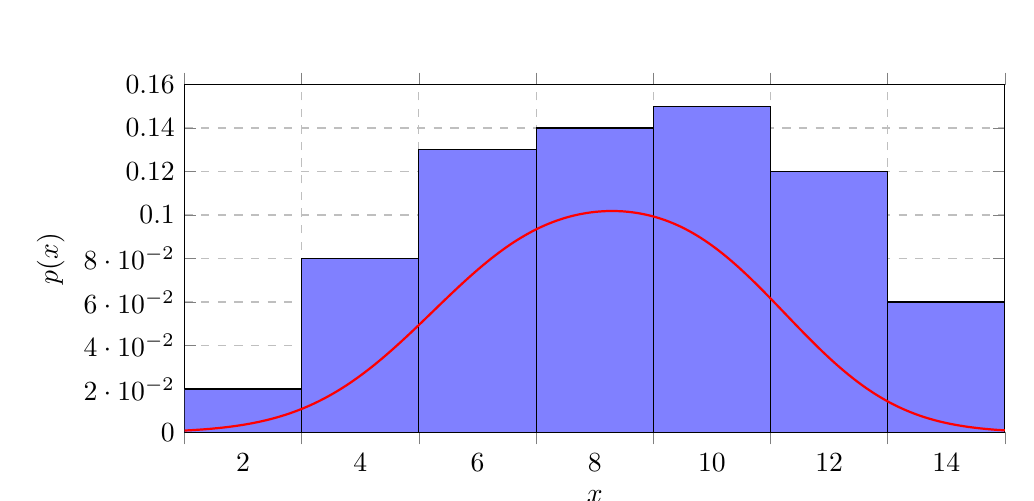
\begin{tikzpicture}
\begin{axis}[
    width=12cm,
    height=6cm,
    ybar interval,
    xmin=2, xmax=16,
    ymin=0, ymax=0.16,
    xlabel={$x$},
    ylabel={$p(x)$},
    xtick={2,4,6,8,10,12,14,16},
    ytick={0,0.02,0.04,0.06,0.08,0.10,0.12,0.14,0.16},
    ymajorgrids=true,
    grid style=dashed,
]
\addplot+[ybar interval, fill=blue!50, draw=black] coordinates {
    (2,0.02) (4,0.08) (6,0.13) (8,0.14) (10,0.15) (12,0.12) (14,0.06) (16,0.02)
};
\addplot[red, thick, smooth, domain=2:16, samples=100] {0.08*exp(-((x-8)^2)/8) + 0.06*exp(-((x-11)^2)/6)};
\end{axis}
\end{tikzpicture}
\end{center}

\subsection{Drawbacks of Histograms}

Despite their simplicity, histograms have several significant limitations:

\begin{enumerate}
    \item \textbf{Dependence on starting position}: The density estimate depends on the starting position of the bins
    \begin{itemize}
        \item Different starting positions can produce different density estimates
        \item For multivariate data, the density estimate is also affected by the \textbf{orientation of the bins}
    \end{itemize}
    
    \item \textbf{Discontinuities}: The discontinuities of the estimate are not due to the underlying density; they are only an artifact of the chosen bin locations
    \begin{itemize}
        \item These discontinuities make it very difficult to grasp the \textbf{structure} of the data
        \item The true underlying distribution is typically smooth, but histograms create artificial jumps
    \end{itemize}
    
    \item \textbf{Curse of dimensionality}: A much more serious problem is the \textbf{curse of dimensionality}, since the number of bins grows exponentially with the number of dimensions
    \begin{itemize}
        \item In high dimensions we would require a very large number of examples or else most of the bins would be empty
        \item With $d$ dimensions and $k$ bins per dimension, we need $k^d$ total bins
    \end{itemize}
\end{enumerate}

\begin{center}
\colorbox{red!15}{\parbox{0.9\textwidth}{
\textbf{The Curse of Dimensionality}\\[0.2cm]
As the number of features or dimensions increases, the amount of data required to effectively cover the feature space increases \textbf{exponentially}.
}}
\end{center}

\subsection{The Curse of Dimensionality}

\begin{definition}[Curse of Dimensionality]
The curse of dimensionality refers to the challenges and issues that arise when working with high-dimensional data in machine learning.

As the number of features or dimensions in a dataset increases, the amount of data required to effectively cover the feature space also increases exponentially.
\end{definition}

\subsubsection{Why It Matters}

\begin{itemize}
    \item \textbf{Exponential growth}: With $d$ dimensions, if each dimension is divided into $k$ bins, we need $k^d$ bins total
    
    \item \textbf{Data sparsity}: In high dimensions, data points become increasingly sparse
    \begin{itemize}
        \item Most bins will be empty unless we have an enormous amount of data
        \item The distance between points increases, making it harder to find meaningful patterns
    \end{itemize}
    
    \item \textbf{Sample size requirements}: To maintain the same density of samples, we need exponentially more data as dimensions increase
\end{itemize}

\begin{example}[Exponential Growth of Bins]
\begin{itemize}
    \item 1D: 10 bins per dimension $\rightarrow$ 10 bins total
    \item 2D: 10 bins per dimension $\rightarrow$ 100 bins total
    \item 3D: 10 bins per dimension $\rightarrow$ 1,000 bins total
    \item 10D: 10 bins per dimension $\rightarrow$ 10,000,000,000 bins total!
\end{itemize}
\end{example}

\subsubsection{Mitigating the Curse of Dimensionality}

To mitigate the curse of dimensionality, various techniques are employed:

\begin{itemize}
    \item \textbf{Feature selection}: Choose only the most relevant features
    
    \item \textbf{Dimensionality reduction}: Techniques like Principal Component Analysis (PCA) reduce the number of dimensions while preserving important characteristics
    
    \item \textbf{Regularization methods}: Add constraints to prevent overfitting in high dimensions
    
    \item \textbf{Domain knowledge}: Use expert knowledge to identify which features are truly important
\end{itemize}

\begin{center}
\colorbox{yellow!20}{\parbox{0.9\textwidth}{
\textbf{Practical Implication}\\[0.2cm]
In practice, nonparametric methods like histograms work well for 1D or 2D data, but become impractical for high-dimensional data. This motivates the development of more sophisticated techniques.
}}
\end{center}

\subsection{Probability Density: Mathematical Foundation}

Before we proceed with more advanced nonparametric techniques, let's return to the basic definition of probability to get a solid idea of what we are trying to accomplish.

\begin{tcolorbox}[colback=cyan!5!white,colframe=cyan!75!black,title=\textbf{Probability in a Region}]
The probability that a vector $\mathbf{x}$, drawn from a distribution $P(\mathbf{x})$, will fall in a region $\mathcal{R}$ of the sample space is:

\[
P = \int_{\mathbf{x}' \in \mathcal{R}} P(\mathbf{x}') \, d\mathbf{x}'
\]

where:
\begin{itemize}
    \item $\mathbf{x}$ is a particular vector we are asking about ("drawn from the distribution")
    \item $\mathbf{x}'$ is a dummy variable used to sum/integrate over all vectors in $\mathcal{R}$
    \item $\mathcal{R}$ is a region in the feature space
\end{itemize}
\end{tcolorbox}

\begin{observation}
This integral formulation is the foundation for all density estimation methods. The key insight is that if we can estimate the probability in small regions around each point, we can reconstruct the entire probability density function.
\end{observation}

\subsubsection{Key Concepts}

\begin{itemize}
    \item \textbf{Probability density function} $P(\mathbf{x})$: Describes how probability is distributed over the feature space
    
    \item \textbf{Integration over a region}: The probability of falling in region $\mathcal{R}$ is the integral of the density over that region
    
    \item \textbf{Dummy variable} $\mathbf{x}'$: Used for integration; represents all possible points in the region
    
    \item \textbf{Normalization}: The integral over the entire space must equal 1:
    \[
    \int_{\text{all space}} P(\mathbf{x}') \, d\mathbf{x}' = 1
    \]
\end{itemize}

\begin{remark}
For discrete distributions, the integral becomes a sum:
\[
P = \sum_{\mathbf{x}' \in \mathcal{R}} P(\mathbf{x}')
\]

This is the discrete analog of the continuous case and is what we use when working with categorical data.
\end{remark}

\subsection{Binomial Distribution Approach}

Now let's develop a more rigorous approach to nonparametric density estimation based on probability theory.

\subsubsection{Setup}

Suppose now that $N$ vectors $\{\mathbf{x}(1), \mathbf{x}(2), \ldots, \mathbf{x}(N)\}$ are drawn \textbf{independently and identically distributed (i.i.d.)} from the distribution. The probability that $k$ of these $N$ vectors fall in $\mathcal{R}$ is given by the binomial distribution:

\begin{tcolorbox}[colback=blue!5!white,colframe=blue!75!black,title=\textbf{Binomial Distribution}]
\[
P(k) = \binom{N}{k} P^k (1-P)^{N-k}
\]

where:
\[
\binom{N}{k} = \frac{N!}{k!(N-k)!}
\]

and the expected value for $k$ is:
\[
\mathbb{E}[k] = NP
\]
\end{tcolorbox}

\begin{observation}
\textbf{Recall}: The expectation is the average value we would get if we repeated drawing samples many times.

The binomial distribution tells us how likely it is to observe exactly $k$ points in region $\mathcal{R}$ when we draw $N$ samples, given that each point has probability $P$ of falling in $\mathcal{R}$.
\end{observation}

\subsubsection{Mean and Variance of the Ratio}

The mean and variance of the ratio $k/N$ are:

\begin{align}
\mathbb{E}\left[\frac{k}{N}\right] &= P \\
\text{Var}\left[\frac{k}{N}\right] &= \mathbb{E}\left[\left(\frac{k}{N} - P\right)^2\right] = \frac{P(1-P)}{N}
\end{align}

\begin{observation}
Therefore, as $N \to \infty$, the distribution becomes \textbf{sharper}, the variance gets \textbf{smaller}, thus we can obtain a \textbf{better estimate} of the probability $P$ from the mean fraction of the points that fall within $\mathcal{R}$:

\[
P \cong \frac{k}{N}
\]

This is the law of large numbers in action: with more samples, our estimate becomes more accurate.
\end{observation}

\subsection{Density Estimation Formula}

\subsubsection{Small Region Assumption}

On the other hand, if we assume that $\mathcal{R}$ is \textbf{so small} that $P(\mathbf{x})$ \textbf{does not vary} appreciably within it, then:

\[
\int_{\mathcal{R}} P(\mathbf{x}') \, d\mathbf{x}' \cong P(\mathbf{x}) V
\]

where $V$ is the \textbf{volume enclosed} by region $\mathcal{R}$.

\begin{observation}
This approximation assumes that the probability density is approximately constant within the small region $\mathcal{R}$, so we can pull $P(\mathbf{x})$ out of the integral, leaving just the volume $V$.
\end{observation}

\subsubsection{Combining the Results}

Merging with the previous result, we obtain:

\begin{align}
P &= \int_{\mathcal{R}} p(\mathbf{x}') \, d\mathbf{x}' \cong p(\mathbf{x}) V \\
P &\cong \frac{k}{N}
\end{align}

Therefore:
\[
p(\mathbf{x}) \cong \frac{k}{NV}
\]

\begin{center}
\colorbox{green!15}{\parbox{0.9\textwidth}{
\centering
\textbf{Key Result}\\[0.2cm]
This estimate becomes more accurate as we \textbf{increase the number of sample points} $N$ and \textbf{shrink the volume} $V$.
}}
\end{center}

\subsection{The Trade-off Problem}

In practice, the value of $N$ (the total number of examples) is fixed.

\subsubsection{The Dilemma}

\begin{itemize}
    \item In order to improve the accuracy of the estimate $P(\mathbf{x})$ we could let $V$ to approach zero, but then the region $\mathcal{R}$ would become so small that it would enclose no examples
    
    \item This means that in practice, we will have to find a \textbf{compromise value of the volume} $V$:
    \begin{itemize}
        \item \textbf{Large enough} to include enough examples within $\mathcal{R}$
        \item \textbf{Small enough} to support the assumption that $P(\mathbf{x})$ is constant within $\mathcal{R}$
    \end{itemize}
\end{itemize}

\begin{center}
\colorbox{red!15}{\parbox{0.9\textwidth}{
\textbf{The Fundamental Trade-off}\\[0.2cm]
\begin{itemize}
    \item Too large $V$ $\rightarrow$ Poor approximation (density varies within region)
    \item Too small $V$ $\rightarrow$ Too few samples (high variance in estimate)
\end{itemize}
}}
\end{center}

\subsection{General Nonparametric Density Estimation Formula}

\begin{tcolorbox}[colback=orange!5!white,colframe=orange!75!black,title=\textbf{General Expression for Nonparametric Density Estimation}]
\[
P(\mathbf{x}) \cong \frac{k}{NV}
\]

where:
\begin{itemize}
    \item $V$ is the volume surrounding $\mathbf{x}$
    \item $N$ is the total number of examples
    \item $k$ is the number of examples inside $V$
\end{itemize}
\end{tcolorbox}

\subsection{Two Approaches to Nonparametric Density Estimation}

When applying this result to practical density estimation problems, two basic approaches can be adopted:

\begin{enumerate}
    \item \textbf{Fix $V$ and determine $k$ from the data}
    \begin{itemize}
        \item This leads to \textbf{kernel density estimation (KDE)}, e.g., Parzen window
        \item We define a fixed-size region around each point and count how many samples fall within it
    \end{itemize}
    
    \item \textbf{Fix $k$ and determine $V$ from the data}
    \begin{itemize}
        \item This gives rise to the \textbf{$k$-nearest-neighbor ($k$-NN) approach}
        \item We find the $k$ nearest neighbors and measure the volume needed to enclose them
    \end{itemize}
\end{enumerate}

\begin{center}
\colorbox{purple!15}{\parbox{0.9\textwidth}{
\textbf{Convergence Property}\\[0.2cm]
Both $k$-NN and KDE converge to the true probability density as $N \to \infty$, provided that:
\begin{itemize}
    \item $V$ shrinks with $N$
    \item $k$ grows with $N$ appropriately
\end{itemize}
}}
\end{center}

\subsubsection{Comparison of Approaches}

\begin{table}[h]
\centering
\begin{tabular}{|p{6cm}|p{6cm}|}
\hline
\textbf{Kernel Density Estimation (KDE)} & \textbf{$k$-Nearest Neighbor ($k$-NN)} \\
\hline
Fix volume $V$ & Fix number of neighbors $k$ \\
Count samples $k$ in fixed region & Adjust volume $V$ to include $k$ samples \\
Smooth density estimate & Adaptive to local density \\
Can be zero in sparse regions & Always uses $k$ neighbors \\
Examples: Parzen window, Gaussian kernel & Examples: $k$-NN classifier, $k$-NN regressor \\
\hline
\end{tabular}
\caption{Comparison of KDE and $k$-NN approaches}
\end{table}

\begin{observation}
\textbf{KDE} produces smoother estimates but may miss structure in sparse regions, while \textbf{$k$-NN} adapts to local density but can produce less smooth estimates. The choice depends on the specific application and data characteristics.
\end{observation}

\subsubsection{Choosing Parameters}

\begin{itemize}
    \item \textbf{For KDE}: Choose bandwidth (related to $V$)
    \begin{itemize}
        \item Too small: noisy, overfitting
        \item Too large: oversmoothing, missing details
    \end{itemize}
    
    \item \textbf{For $k$-NN}: Choose $k$
    \begin{itemize}
        \item Too small: sensitive to noise, high variance
        \item Too large: oversmoothing, high bias
    \end{itemize}
\end{itemize}

\begin{remark}
Both methods require careful tuning of their parameters (bandwidth for KDE, $k$ for $k$-NN). Cross-validation is commonly used to select these parameters in practice.
\end{remark}

\section{k-Nearest Neighbors (k-NN)}

\subsection{Visual Comparison: k-NN vs. Parzen Windows}

\begin{center}
\colorbox{blue!15}{\parbox{0.9\textwidth}{
\textbf{Key Difference:}
\begin{itemize}
    \item \textbf{Parzen Window}: Fixed volume $V$ (radius $R$), variable $k$
    \item \textbf{k-NN}: Fixed $k$ (number of neighbors), variable volume $V$ (radius $R$)
\end{itemize}
}}
\end{center}

\begin{observation}
In the visual comparison:
\begin{itemize}
    \item \textbf{Parzen Window}: Uses a fixed-size circle (radius $R$) around the query point (yellow cross). The number of points inside varies depending on local density.
    
    \item \textbf{k-NN (e.g., 3-NN)}: The circle grows or shrinks to always include exactly $k=3$ nearest neighbors. In dense regions, the circle is small; in sparse regions, it's large.
\end{itemize}
\end{observation}

\subsection{Parzen Window: Practical Considerations}

\begin{center}
\colorbox{orange!15}{\parbox{0.9\textwidth}{
\textbf{When to Use Parzen Windows}\\[0.2cm]
Parzen window is great for \textbf{low-dimensional data} (2–3 features, maybe up to 5).
}}
\end{center}

\begin{itemize}
    \item In higher dimensions, the method becomes \textbf{computationally expensive}, and the density estimates are \textbf{unreliable} because of the curse of dimensionality
    
    \item For this reason, in A.A. 2025–2026, we focus on other methods better suited for high-dimensional data
\end{itemize}

\begin{remark}
While Parzen windows provide smooth density estimates, they suffer from the curse of dimensionality. As dimensions increase, the fixed window size becomes either too large (oversmoothing) or too small (too few samples), making the method impractical for modern high-dimensional datasets.
\end{remark}

\subsection{k-Nearest Neighbors Algorithm}

The k-NN algorithm is one of the simplest and most intuitive machine learning algorithms.

\subsubsection{Basic Principle}

The volume is grown surrounding the estimation point $\mathbf{x}$, until it encloses a total of $k$ data points.

\begin{center}
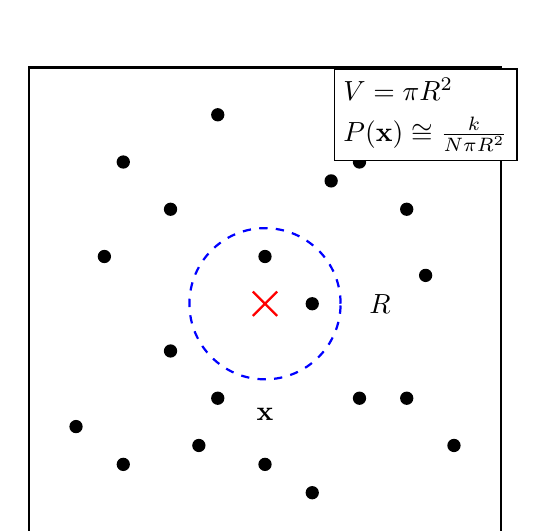
\begin{tikzpicture}[scale=1.2]
% Draw boundary
\draw[thick] (0,0) rectangle (5,5);

% Draw scattered points
\foreach \x/\y in {0.5/1.2, 1.0/0.8, 1.5/2.0, 2.0/1.5, 2.5/3.0, 3.0/2.5, 3.5/4.0, 4.0/3.5, 4.5/1.0, 1.0/4.0, 2.0/4.5, 3.0/0.5, 4.0/1.5, 1.5/3.5, 3.5/1.5, 2.5/0.8, 0.8/3.0, 4.2/2.8, 1.8/1.0, 3.2/3.8}
{
    \fill (\x,\y) circle (2pt);
}

% Query point
\node[cross out, draw=red, thick, minimum size=8pt] at (2.5,2.5) {};

% Circle around query point
\draw[dashed, thick, blue] (2.5,2.5) circle (0.8);

% Label
\node[right] at (3.5,2.5) {$R$};
\node[below] at (2.5,1.5) {$\mathbf{x}$};

% Formula
\node[align=left, draw, fill=white] at (4.2,4.5) {$V = \pi R^2$\\[0.1cm]$P(\mathbf{x}) \cong \frac{k}{N \pi R^2}$};
\end{tikzpicture}
\end{center}

\begin{tcolorbox}[colback=green!5!white,colframe=green!75!black,title=\textbf{k-NN Density Estimation}]
\[
P(\mathbf{x}) \cong \frac{k}{NV}
\]

where:
\begin{itemize}
    \item $V$ is the volume surrounding $\mathbf{x}$
    \item $N$ is the total number of examples
    \item $k$ is the number of examples inside $V$ (fixed)
\end{itemize}
\end{tcolorbox}

\subsection{k-NN for Classification}

\subsubsection{1-Nearest Neighbor (1-NN)}

Given an unknown point $\mathbf{x}^*$, we consider $s_i \in \{s_1, \ldots, s_N\} = S$ the nearest point (NN) of the point $\mathbf{x}^*$ if:

\[
d(\mathbf{x}^*, s_i) = \min_l d(\mathbf{x}^*, s_l), \quad l = 1 \ldots N
\]

where $d(\cdot)$ is a \textbf{distance measure} defined on the feature space.

\begin{observation}
If you interpret each point of set $S$ as a prototype of a class, you can then see the equation above as a rule of classification \textbf{1-NN} associating the sample $\mathbf{x}$ to the class $j$ to which the point $s_i$ belongs.
\end{observation}

\begin{example}[Common Distance Measures]

    
\begin{itemize}
    \item \textbf{Euclidean distance}: $d(\mathbf{x}, \mathbf{y}) = \sqrt{\sum_{i=1}^{d} (x_i - y_i)^2}$
    
    \item \textbf{Manhattan distance}: $d(\mathbf{x}, \mathbf{y}) = \sum_{i=1}^{d} |x_i - y_i|$
    
    \item \textbf{Minkowski distance}: $d(\mathbf{x}, \mathbf{y}) = \left(\sum_{i=1}^{d} |x_i - y_i|^p\right)^{1/p}$
\end{itemize}
\end{example}

\subsubsection{Generalizing to k-NN}

Rule 1-NN can be generalised to define a \textbf{$k$-NN rule}, which consists of determining the $k$ points belonging to the set $S$ closest to the observation $\mathbf{x}$.

\begin{tcolorbox}[colback=purple!5!white,colframe=purple!75!black,title=\textbf{k-NN Classification Rule}]
The classification rule $k$-NN associates observation $\mathbf{x}$ with class $i$ having the \textbf{largest number of elements} among the nearest $k$.

We call $U(\mathbf{x})$ the set of $k$ points closer to $\mathbf{x}$.
\end{tcolorbox}

\subsubsection{Majority Voting}

For example, with odd $k$ and two classes, $y_1$ and $y_2$, the decision rule can choose the class with the most samples in $U(\mathbf{x})$. This is called \textbf{majority voting}.

\begin{center}
\colorbox{cyan!15}{\parbox{0.9\textwidth}{
\centering
\textbf{Majority Voting}\\[0.2cm]
Choose the class that appears most frequently among the $k$ nearest neighbors.
}}
\end{center}

\begin{example}[3-NN Classification]
Suppose we have $k=3$ and two classes (red and blue):
\begin{itemize}
    \item Query point $\mathbf{x}^*$ has 3 nearest neighbors: 2 red, 1 blue
    \item Majority voting: $\mathbf{x}^*$ is classified as \textbf{red}
\end{itemize}
\end{example}

\subsection{Choosing k}

The choice of $k$ is critical for k-NN performance:

\begin{table}[h]
\centering
\begin{tabular}{|p{3cm}|p{5cm}|p{5cm}|}
\hline
\textbf{Value of k} & \textbf{Advantages} & \textbf{Disadvantages} \\
\hline
Small $k$ (e.g., 1-3) & 
- Captures local structure\\
- More flexible decision boundaries & 
- Sensitive to noise\\
- High variance\\
- Overfitting \\
\hline
Large $k$ & 
- More robust to noise\\
- Smoother decision boundaries\\
- Lower variance & 
- May miss local patterns\\
- High bias\\
- Underfitting \\
\hline
Odd $k$ & 
- Avoids ties in binary classification & 
- \\
\hline
\end{tabular}
\caption{Trade-offs in choosing $k$}
\end{table}

\begin{center}
\colorbox{yellow!20}{\parbox{0.9\textwidth}{
\textbf{Rule of Thumb}\\[0.2cm]
\begin{itemize}
    \item Start with $k = \sqrt{N}$ where $N$ is the number of training samples
    \item Use cross-validation to find the optimal $k$
    \item For binary classification, use odd $k$ to avoid ties
\end{itemize}
}}
\end{center}

\subsection{Advantages and Disadvantages of k-NN}

\begin{table}[h]
\centering
\begin{tabular}{|p{7cm}|p{7cm}|}
\hline
\textbf{Advantages} & \textbf{Disadvantages} \\
\hline
$\bullet$ Simple and intuitive & $\bullet$ Computationally expensive at prediction time \\
$\bullet$ No training phase (lazy learning) & $\bullet$ Requires storing all training data \\
$\bullet$ Naturally handles multi-class problems & $\bullet$ Sensitive to irrelevant features \\
$\bullet$ Non-parametric (no assumptions about data distribution) & $\bullet$ Sensitive to the scale of features \\
$\bullet$ Can capture complex decision boundaries & $\bullet$ Curse of dimensionality \\
$\bullet$ Easy to update with new data & $\bullet$ Choosing optimal $k$ can be difficult \\
\hline
\end{tabular}
\caption{Advantages and disadvantages of k-NN}
\end{table}

\subsection{Practical Considerations}

\subsubsection{Feature Scaling}

\begin{observation}
k-NN is \textbf{highly sensitive to feature scaling} because it relies on distance calculations. Features with larger ranges will dominate the distance metric.
\end{observation}

\textbf{Solution}: Always normalize or standardize features before applying k-NN:
\begin{itemize}
    \item \textbf{Min-Max Normalization}: Scale to $[0, 1]$: $x' = \frac{x - \min(x)}{\max(x) - \min(x)}$
    
    \item \textbf{Standardization}: Scale to mean 0, std 1: $x' = \frac{x - \mu}{\sigma}$
\end{itemize}

\subsubsection{Computational Complexity}

\begin{itemize}
    \item \textbf{Training time}: $O(1)$ (no training, just store data)
    \item \textbf{Prediction time}: $O(Nd)$ where $N$ is training set size, $d$ is dimensionality
    \item For large datasets, use approximate nearest neighbor algorithms (e.g., KD-trees, Ball trees, LSH)
\end{itemize}

\begin{remark}
k-NN is called a \textbf{lazy learner} or \textbf{instance-based learner} because it doesn't learn a model during training. Instead, it memorizes the training data and performs all computation at prediction time. This makes training fast but prediction slow, especially for large datasets.
\end{remark}

\subsection{Distance Metrics in k-NN}

\subsubsection{Euclidean Distance}

To calculate the distance, we usually use \textbf{Euclidean distance}.

\begin{center}
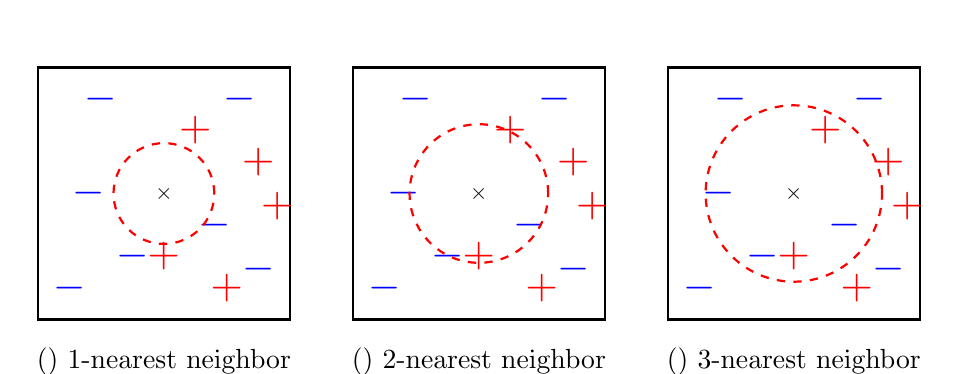
\begin{tikzpicture}[scale=0.8]
% Three subfigures showing 1-NN, 2-NN, 3-NN
\foreach \k/\xshift in {1/0, 2/5, 3/10} {
    \begin{scope}[shift={(\xshift,0)}]
        % Draw frame
        \draw[thick] (0,0) rectangle (4,4);
        
        % Draw blue minus points
        \foreach \x/\y in {0.5/0.5, 1.0/3.5, 0.8/2.0, 1.5/1.0, 3.5/0.8, 3.2/3.5, 2.8/1.5} {
            \node[blue, scale=1.5] at (\x,\y) {$-$};
        }
        
        % Draw red plus points
        \foreach \x/\y in {3.0/0.5, 3.5/2.5, 2.5/3.0, 2.0/1.0, 3.8/1.8} {
            \node[red, scale=1.5] at (\x,\y) {$+$};
        }
        
        % Query point
        \node[scale=0.8] at (2,2) {$\times$};
        
        % Draw circle
        \pgfmathsetmacro{\radius}{0.5 + \k*0.3}
        \draw[red, dashed, thick] (2,2) circle (\radius);
        
        % Label
        \node[below] at (2,-0.3) {(\alph{figure}) \k-nearest neighbor};
    \end{scope}
}
\end{tikzpicture}
\end{center}

\begin{tcolorbox}[colback=blue!5!white,colframe=blue!75!black,title=\textbf{Euclidean Distance Formula}]
Given two points $\mathbf{p} = (p_1, p_2, \ldots, p_n)$ and $\mathbf{q} = (q_1, q_2, \ldots, q_n)$:

\[
d(\mathbf{p}, \mathbf{q}) = \sqrt{(q_1 - p_1)^2 + (q_2 - p_2)^2 + \ldots + (q_n - p_n)^2} = \sqrt{\sum_{i=1}^{n} (q_i - p_i)^2}
\]
\end{tcolorbox}

\begin{observation}
The visual shows how the radius grows as $k$ increases:
\begin{itemize}
    \item \textbf{1-NN}: Small circle, includes only the closest neighbor
    \item \textbf{2-NN}: Medium circle, includes 2 closest neighbors
    \item \textbf{3-NN}: Larger circle, includes 3 closest neighbors
\end{itemize}
The decision boundary depends on which class dominates within the circle.
\end{observation}

\subsection{Weighted k-NN}

\subsubsection{The Problem with Equal Weights}

All the closest neighbors have the same weights, meaning that they are equally important to make a decision.

\begin{center}
\colorbox{red!15}{\parbox{0.9\textwidth}{
\textbf{Issue:} Therefore, the algorithm is very sensitive to the number of $k$.
}}
\end{center}

\subsubsection{Solution: Distance-Based Weighting}

This can be reduced by \textbf{weighing the contribution of neighbors based on distance} $w = 1/d(\mathbf{x}^*, s_i)$, such that the \textbf{closest} neighbor would have more \textbf{importance}.

\begin{tcolorbox}[colback=green!5!white,colframe=green!75!black,title=\textbf{Weighted k-NN}]
Instead of simple majority voting, each neighbor contributes with weight:
\[
w_i = \frac{1}{d(\mathbf{x}^*, s_i)}
\]

The class with the highest weighted sum is chosen:
\[
\text{class}(\mathbf{x}^*) = \arg\max_c \sum_{i \in U(\mathbf{x}^*)} w_i \cdot \mathbb{1}(y_i = c)
\]

where $\mathbb{1}(y_i = c)$ is 1 if neighbor $i$ belongs to class $c$, and 0 otherwise.
\end{tcolorbox}

\begin{example}[Weighted vs. Unweighted k-NN]
Consider $k=3$ with neighbors at distances 1, 2, and 5:
\begin{itemize}
    \item \textbf{Unweighted}: Each neighbor gets weight 1
    \item \textbf{Weighted}: Neighbors get weights $w_1 = 1/1 = 1.0$, $w_2 = 1/2 = 0.5$, $w_3 = 1/5 = 0.2$
\end{itemize}
The closest neighbor has much more influence in the weighted version.
\end{example}

\subsection{Importance of Feature Scaling (Revisited)}

\subsubsection{Why k is Sensitive}

The choice of $k$ is important because:
\begin{itemize}
    \item If $k$ is too \textbf{small}, the approach is \textbf{sensitive to noise}
    \item If $k$ is too \textbf{large}, the neighborhood can include examples belonging to \textbf{other classes}
\end{itemize}

\begin{center}
\colorbox{yellow!20}{\parbox{0.9\textwidth}{
\textbf{Critical Requirement}\\[0.2cm]
To operate correctly the attributes must have the \textbf{same value scale} and must therefore be \textbf{normalized} in the preprocessing phase.
}}
\end{center}

\begin{observation}
Without normalization, features with larger ranges will dominate the distance calculation, making features with smaller ranges essentially irrelevant to the classification decision.
\end{observation}

\subsection{Mahalanobis Distance}

\subsubsection{When Euclidean Distance is Not Enough}

Normalizing the scale may not be sufficient when there are different data distributions.

\begin{center}
\colorbox{orange!15}{\parbox{0.9\textwidth}{
In such cases instead of using Euclidean distance, one can also try using \textbf{Mahalanobis distance}.
}}
\end{center}

\subsubsection{Definition}

The Mahalanobis distance is a measure of the distance between \textbf{a point and a distribution}. It's a generalized form of the Euclidean distance that accounts for \textbf{correlations between variables} and \textbf{different variances} along different axes.

\begin{tcolorbox}[colback=purple!5!white,colframe=purple!75!black,title=\textbf{Mahalanobis Distance Formula}]
\[
D = \sqrt{(\mathbf{x} - \boldsymbol{\mu})^T \boldsymbol{\Sigma}^{-1} (\mathbf{x} - \boldsymbol{\mu})}
\]

where:
\begin{itemize}
    \item $\mathbf{x}$ is the $n$-dimensional vector representing the point's coordinates
    \item $\boldsymbol{\mu}$ is the $n$-dimensional vector representing the mean of the distribution
    \item $\boldsymbol{\Sigma}$ is the $n \times n$ covariance matrix of the distribution
    \item $\boldsymbol{\Sigma}^{-1}$ is the inverse of the covariance matrix
\end{itemize}
\end{tcolorbox}

\begin{observation}
When the covariance matrix is the identity matrix (i.e., features are uncorrelated and have unit variance), the Mahalanobis distance reduces to the Euclidean distance.
\end{observation}

\subsubsection{When to Use Mahalanobis Distance}

\begin{enumerate}
    \item \textbf{Correlated Features}: Changes in one feature are associated with changes in another.
    
    \item \textbf{Unequal Variances}: MD normalizes the distance based on the variances of the features, preventing features with larger variances from dominating the distance calculation.
    
    \item \textbf{Outlier Detection}: Outliers often have a large MD from the rest of the data points, especially if they deviate from the normal covariance pattern.
    
    \item \textbf{In high dimensional spaces}: ED can be problematic (\textit{curse of dimensionality}). Incorporating information about the covariance structure, can mitigate this issue to some extent.
\end{enumerate}

\begin{table}[h]
\centering
\begin{tabular}{|p{7cm}|p{7cm}|}
\hline
\textbf{Euclidean Distance} & \textbf{Mahalanobis Distance} \\
\hline
Assumes features are independent & Accounts for correlations between features \\
\hline
Treats all directions equally & Accounts for different variances along different axes \\
\hline
Sensitive to feature scaling & Automatically accounts for different scales \\
\hline
Simple and fast to compute & More computationally expensive (requires covariance matrix) \\
\hline
Works well when features are uncorrelated and have similar variance & Better when features are correlated or have different variances \\
\hline
Distance from point to point & Distance from point to distribution \\
\hline
\end{tabular}
\caption{Euclidean vs. Mahalanobis Distance}
\end{table}

\begin{example}[Mahalanobis Distance in Practice]
Consider a 2D dataset where:
\begin{itemize}
    \item Feature 1 has variance 1
    \item Feature 2 has variance 100
    \item Features are positively correlated
\end{itemize}

\textbf{Euclidean distance} would be dominated by Feature 2 due to its large variance.

\textbf{Mahalanobis distance} would:
\begin{itemize}
    \item Normalize for the different variances
    \item Account for the correlation structure
    \item Provide a more meaningful distance measure
\end{itemize}
\end{example}

\begin{remark}
Computing Mahalanobis distance requires estimating the covariance matrix $\boldsymbol{\Sigma}$, which can be challenging when:
\begin{itemize}
    \item The number of features is large relative to the number of samples
    \item The covariance matrix is singular (not invertible)
    \item There is insufficient data to reliably estimate correlations
\end{itemize}
In such cases, regularization techniques or dimensionality reduction may be needed before applying Mahalanobis distance.
\end{remark}

\subsubsection{Visual Example: Euclidean vs. Mahalanobis Distance}

\begin{example}[Comparing Distance Metrics]
Consider a dataset with a centroid at $(\bar{x}, \bar{y}) = (3.1, 3.0)$ and two data points:
\begin{itemize}
    \item \textbf{Data point 1}: $(5, 5)$ (yellow/orange point)
    \item \textbf{Data point 2}: $(5, 1)$ (blue point)
\end{itemize}

\textbf{Using Euclidean Distance:}

Distance from centroid to Data point 1:
\[
d_1 = \sqrt{(5-3.1)^2 + (5-3.0)^2} = \sqrt{1.9^2 + 2.0^2} = \sqrt{3.61 + 4.00} = 2.76
\]

Distance from centroid to Data point 2:
\[
d_2 = \sqrt{(5-3.1)^2 + (1-3.0)^2} = \sqrt{1.9^2 + (-2.0)^2} = \sqrt{3.61 + 4.00} = 2.76
\]

\begin{center}
\colorbox{purple!15}{\parbox{0.9\textwidth}{
\centering
\textbf{Based on Euclidean distance, both points have the same distance to the centroid!}
}}
\end{center}
\end{example}

\begin{observation}
However, looking at the scatter plot, we can see that the green points (the cluster) are elongated along a diagonal direction. Data point 1 lies along this diagonal trend, while Data point 2 deviates significantly from it.

Euclidean distance treats all directions equally and doesn't account for the correlation structure of the data.
\end{observation}

\begin{example}[Using Mahalanobis Distance]
When we apply Mahalanobis distance to the same scenario:

\begin{itemize}
    \item \textbf{MD$_1$ = 2.26} (Data point 1 to centroid)
    \item \textbf{MD$_2$ = 6.45} (Data point 2 to centroid)
\end{itemize}

\begin{center}
\colorbox{orange!15}{\parbox{0.9\textwidth}{
\textbf{Why is MD$_1$ so different from MD$_2$?}\\[0.2cm]
Because MD takes into account the \textbf{correlation} in the data.
}}
\end{center}

\textbf{Interpretation:}
\begin{itemize}
    \item Data point 1 follows the natural diagonal trend of the cluster $\rightarrow$ smaller Mahalanobis distance
    \item Data point 2 deviates from the correlation pattern $\rightarrow$ larger Mahalanobis distance
\end{itemize}
\end{example}

\begin{remark}
This example illustrates why Mahalanobis distance is superior when features are correlated:
\begin{itemize}
    \item \textbf{Euclidean distance}: Treats both points as equally distant (2.76)
    \item \textbf{Mahalanobis distance}: Correctly identifies that point 2 is much farther from the distribution (6.45 vs 2.26)
\end{itemize}
Mahalanobis distance accounts for the shape and orientation of the data distribution, not just raw coordinate distances.
\end{remark}

\subsection{How to Select k in k-NN}

Choosing the right value of $k$ is crucial for k-NN performance. Here are practical strategies:

\subsubsection{Common Heuristics}

\begin{itemize}
    \item \textbf{Common values}: Often 3, 5, 7
    
    \item \textbf{Choose an odd number} to avoid ties (\textit{undetermined cases})
    
    \item \textbf{Use your training and validation data} to decide $k$:
    \begin{itemize}
        \item Change $k$ from $k=1$ until the validation performance decreases
        \item Pay attention not to \textbf{underfit} and \textbf{overfit} the data
        \item Finalize the decision of $k$ and use the same $k$ to classify the test data
    \end{itemize}
    
    \item \textbf{A typical choice} is $k \approx \sqrt{N}$ where $N$ is the number of training samples
\end{itemize}

\begin{center}
\colorbox{yellow!20}{\parbox{0.9\textwidth}{
\textbf{Validation-Based Selection}\\[0.2cm]
The most reliable method is to use cross-validation:
\begin{enumerate}
    \item Try different values of $k$ (e.g., 1, 3, 5, 7, 9, 11, ...)
    \item Evaluate performance on validation set for each $k$
    \item Select the $k$ that gives the best validation performance
    \item Use this optimal $k$ on the test set
\end{enumerate}
}}
\end{center}

\subsubsection{Visual Understanding: k and Decision Boundaries}

\begin{center}
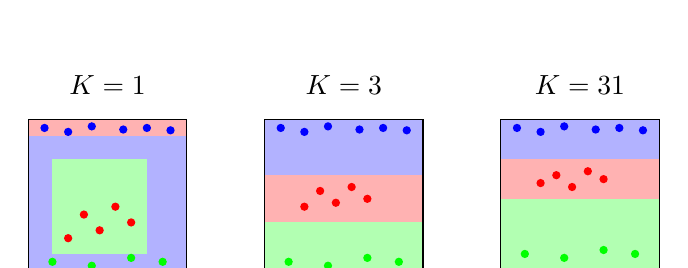
\begin{tikzpicture}[scale=1.0]
% K=1
\begin{scope}[shift={(0,0)}]
    \node[above] at (1,2.2) {$K=1$};
    \draw[thick] (0,0) rectangle (2,2);
    \fill[blue!30] (0,0) rectangle (2,2);
    \fill[green!30] (0.3,0.3) -- (1.5,0.3) -- (1.5,1.5) -- (0.3,1.5) -- cycle;
    \fill[red!30] (0,1.8) rectangle (2,2);
    
    % Points
    \foreach \x/\y in {0.2/1.9, 0.5/1.85, 0.8/1.92, 1.2/1.88, 1.5/1.9, 1.8/1.87} {
        \fill[blue] (\x,\y) circle (1.5pt);
    }
    \foreach \x/\y in {0.5/0.5, 0.7/0.8, 0.9/0.6, 1.1/0.9, 1.3/0.7} {
        \fill[red] (\x,\y) circle (1.5pt);
    }
    \foreach \x/\y in {0.3/0.2, 0.8/0.15, 1.3/0.25, 1.7/0.2} {
        \fill[green] (\x,\y) circle (1.5pt);
    }
\end{scope}

% K=3
\begin{scope}[shift={(3,0)}]
    \node[above] at (1,2.2) {$K=3$};
    \draw[thick] (0,0) rectangle (2,2);
    \fill[blue!30] (0,1.3) rectangle (2,2);
    \fill[green!30] (0,0) rectangle (2,0.7);
    \fill[red!30] (0,0.7) rectangle (2,1.3);
    
    % Points
    \foreach \x/\y in {0.2/1.9, 0.5/1.85, 0.8/1.92, 1.2/1.88, 1.5/1.9, 1.8/1.87} {
        \fill[blue] (\x,\y) circle (1.5pt);
    }
    \foreach \x/\y in {0.5/0.9, 0.7/1.1, 0.9/0.95, 1.1/1.15, 1.3/1.0} {
        \fill[red] (\x,\y) circle (1.5pt);
    }
    \foreach \x/\y in {0.3/0.2, 0.8/0.15, 1.3/0.25, 1.7/0.2} {
        \fill[green] (\x,\y) circle (1.5pt);
    }
\end{scope}

% K=31
\begin{scope}[shift={(6,0)}]
    \node[above] at (1,2.2) {$K=31$};
    \draw[thick] (0,0) rectangle (2,2);
    \fill[blue!30] (0,1.5) rectangle (2,2);
    \fill[green!30] (0,0) rectangle (2,1.0);
    \fill[red!30] (0,1.0) rectangle (2,1.5);
    
    % Points
    \foreach \x/\y in {0.2/1.9, 0.5/1.85, 0.8/1.92, 1.2/1.88, 1.5/1.9, 1.8/1.87} {
        \fill[blue] (\x,\y) circle (1.5pt);
    }
    \foreach \x/\y in {0.5/1.2, 0.7/1.3, 0.9/1.15, 1.1/1.35, 1.3/1.25} {
        \fill[red] (\x,\y) circle (1.5pt);
    }
    \foreach \x/\y in {0.3/0.3, 0.8/0.25, 1.3/0.35, 1.7/0.3} {
        \fill[green] (\x,\y) circle (1.5pt);
    }
\end{scope}
\end{tikzpicture}
\end{center}

\begin{center}
\colorbox{cyan!15}{\parbox{0.9\textwidth}{
\textbf{What is the role of $k$? How does it relate to overfitting and underfitting?}
}}
\end{center}

\begin{itemize}
    \item \textbf{$k=1$} (left): Very complex, jagged decision boundaries
    \begin{itemize}
        \item High variance, low bias
        \item \textbf{Overfitting}: Captures noise in the training data
        \item Sensitive to outliers
    \end{itemize}
    
    \item \textbf{$k=3$} (middle): Moderate complexity, smoother boundaries
    \begin{itemize}
        \item Balanced bias-variance trade-off
        \item Good generalization
    \end{itemize}
    
    \item \textbf{$k=31$} (right): Very smooth, simple decision boundaries
    \begin{itemize}
        \item Low variance, high bias
        \item \textbf{Underfitting}: May miss important patterns
        \item Too much smoothing
    \end{itemize}
\end{itemize}

\begin{observation}
As $k$ increases:
\begin{itemize}
    \item Decision boundaries become smoother and simpler
    \item The model becomes less sensitive to individual data points
    \item Risk shifts from overfitting (small $k$) to underfitting (large $k$)
\end{itemize}
\end{observation}

\subsubsection{Handling Ties (Undetermined Cases)}

If there are undetermined cases (ties), there are some alternatives:

\begin{enumerate}
    \item \textbf{Arbitrary choice}: Randomly select one of the tied classes
    
    \item \textbf{Nearest average sample}: Assign $\mathbf{x}$ to the class (among those "tie") that has the nearest average sample (calculated between the $k_i$ samples)
    
    \item \textbf{Least distance}: Assign $\mathbf{x}$ to the class that has the $k_i$ samples with least distance from it
\end{enumerate}

\begin{example}[Handling a Tie]
Suppose $k=4$ and we have:
\begin{itemize}
    \item 2 neighbors from class A at distances: 1.5, 2.0
    \item 2 neighbors from class B at distances: 1.2, 3.5
\end{itemize}

\textbf{Solutions:}
\begin{itemize}
    \item \textbf{Arbitrary}: Randomly choose A or B
    \item \textbf{Nearest average}: 
    \begin{itemize}
        \item Class A average: $(1.5 + 2.0)/2 = 1.75$
        \item Class B average: $(1.2 + 3.5)/2 = 2.35$
        \item Choose class A (smaller average distance)
    \end{itemize}
    \item \textbf{Least distance}: Choose class B (has the closest neighbor at 1.2)
\end{itemize}
\end{example}

\begin{remark}
The best strategy for handling ties depends on your specific problem:
\begin{itemize}
    \item \textbf{Nearest average}: Good when you want to consider all neighbors equally
    \item \textbf{Least distance}: Good when you believe the closest neighbor is most important
    \item \textbf{Best practice}: Use odd $k$ to avoid ties altogether in binary classification
\end{itemize}
\end{remark}

\subsection{k-NN: Pros and Cons}

\subsubsection{Advantages (Pros)}

\begin{itemize}
    \item \textbf{Almost no assumptions about the data}
    \begin{itemize}
        \item Non-parametric method
        \item Doesn't assume any particular distribution
        \item Works with any data structure
    \end{itemize}
    
    \item \textbf{Non-parametric}
    \begin{itemize}
        \item No model parameters to learn
        \item Flexible and adaptive to data
    \end{itemize}
    
    \item \textbf{There is no training phase, cost is 0}
    \begin{itemize}
        \item Instant "training" - just store the data
        \item Easy to update with new data
        \item No convergence issues
    \end{itemize}
    
    \item \textbf{Allow us to construct non-linear class boundaries and are therefore more flexible}
    \begin{itemize}
        \item Can capture complex decision boundaries
        \item Not limited to linear separability
        \item Adapts to local data structure
    \end{itemize}
\end{itemize}

\begin{center}
\colorbox{green!15}{\parbox{0.9\textwidth}{
\textbf{k-NN gives locally defined decision boundaries between classes}\\[0.2cm]
Unlike global methods (e.g., linear classifiers), k-NN creates decision boundaries that adapt to the local structure of the data, allowing for complex, non-linear separations.
}}
\end{center}

\begin{observation}
The figure shows how k-NN can create complex, non-linear decision boundaries (shown in red) that follow the natural clustering of the data. The decision boundary is not a simple line or hyperplane, but rather a complex curve that adapts to the local density and distribution of each class (label 1, 2, and 3).

On the right, we see the resulting decision regions where each color represents the area classified as a particular label. The boundaries are highly non-linear and follow the intricate patterns in the data.
\end{observation}

\subsubsection{Disadvantages (Cons)}

\begin{itemize}
    \item \textbf{Need to handle missing data}
    \begin{itemize}
        \item Cannot compute distances with missing values
        \item Requires imputation or special handling
    \end{itemize}
    
    \item \textbf{The distance metric should be chosen carefully}
    \begin{itemize}
        \item Different metrics can give very different results
        \item Must consider feature correlations and scales
        \item May need domain knowledge
    \end{itemize}
    
    \item \textbf{Sensitive to class outliers} (e.g., mislabeled training instances)
    \begin{itemize}
        \item Outliers can create incorrect local decision boundaries
        \item No mechanism to detect or remove bad training examples
    \end{itemize}
    
    \item \textbf{Sensitive to many irrelevant attributes} (which influence the distance)
    \begin{itemize}
        \item All features contribute equally to distance
        \item Irrelevant features add noise
        \item Feature selection is crucial
    \end{itemize}
    
    \item \textbf{Computationally expensive:}
    \begin{itemize}
        \item \textbf{Poor scalability}: For each new example, we have to perform as many comparisons as there are labeled data
        
        \item \textbf{It is necessary to store all data points}: Therefore, the method is more appropriate when the number of samples $N$ is low
        
        \item Memory requirements grow linearly with dataset size
        \item Prediction time is $O(Nd)$ where $N$ is training size, $d$ is dimensionality
    \end{itemize}
\end{itemize}

\begin{center}
\colorbox{red!15}{\parbox{0.9\textwidth}{
\textbf{Scalability Issue}\\[0.2cm]
k-NN does not scale well to large datasets. For a dataset with millions of samples, making a single prediction requires computing distances to all training points, which becomes prohibitively expensive.
}}
\end{center}

\begin{remark}
The main trade-off with k-NN is between flexibility and computational cost:
\begin{itemize}
    \item \textbf{Pros}: Simple, flexible, no training, handles non-linear boundaries
    \item \textbf{Cons}: Slow predictions, high memory, sensitive to irrelevant features and outliers
\end{itemize}

k-NN works best for:
\begin{itemize}
    \item Small to medium-sized datasets
    \item Problems where decision boundaries are complex and non-linear
    \item Applications where training time is critical but prediction time is less important
    \item Situations where new data arrives frequently (easy to update)
\end{itemize}
\end{remark}

\subsection{How k-NN Was Born: PDF Estimation}

k-NN has a theoretical foundation in probability density function (PDF) estimation. Let's explore this connection.

\subsubsection{Going Back to PDF Estimation}

Recall from our earlier discussion of density estimation:

\begin{itemize}
    \item Instead of fixing $V$ as in the case of kernels (Parzen windows), we \textbf{fix the value of $k$} and enlarge the radius of the sphere to include $k$ samples
    
    \item Let's see the \textbf{a-priori probability}:
    \begin{itemize}
        \item Given a class $y_j$, the frequency of occurrence of samples $N_j$ of class $j$ is generally simply measured in relation to the total number of samples $N$, i.e.,
        
        \[
        P(y_j) \equiv \hat{p}(y_j) = \frac{N_j}{N}
        \]
    \end{itemize}
\end{itemize}

\begin{observation}
This is the empirical estimate of the prior probability: the proportion of training samples that belong to class $j$.
\end{observation}

\subsubsection{Density Estimation and Nearest-Neighbor Rule}

Consider 2 classes, $y_i$ and $y_j$, containing $N_i$ and $N_j$ samples, $N = N_i + N_j$.

The local density estimation for $y_i$ is calculated as (and similarly for $y_j$):

\[
\hat{p}(\mathbf{x}|y_i) = \frac{1}{V} \frac{k_i}{N_i}
\]

such that the ratio of $k_i$ ($k_j$) points to the total $N_i$ ($N_j$) belonging to the class $y_i$ ($y_j$) contained in the volume $V$.

\begin{tcolorbox}[colback=blue!5!white,colframe=blue!75!black,title=\textbf{Deriving k-NN from Bayes Rule}]
The Bayes rule says $p(\mathbf{x}|y_i)P(y_i) > p(\mathbf{x}|y_j)P(y_j)$, then

\begin{align*}
\hat{p}(\mathbf{x}|y_i)\hat{p}(y_i) &> \hat{p}(\mathbf{x}|y_j)\hat{p}(y_j) \\
\Rightarrow \frac{1}{V} \frac{k_i}{N_i} \cdot \frac{N_i}{N} &> \frac{1}{V} \frac{k_j}{N_j} \cdot \frac{N_j}{N} \\
\Rightarrow \frac{1}{V N_i} k_i N_i &> \frac{1}{V N_j} k_j N_j \\
\Rightarrow k_i &> k_j
\end{align*}
\end{tcolorbox}

\begin{center}
\colorbox{purple!15}{\parbox{0.9\textwidth}{
\textbf{The k-NN Rule}\\[0.2cm]
Classify $\mathbf{x}$ to class $y_i$ if $k_i > k_j$, i.e., if there are more neighbors from class $i$ than from class $j$ in the volume $V$ around $\mathbf{x}$.
}}
\end{center}

\begin{observation}
This derivation shows that k-NN is actually implementing a Bayesian decision rule using local density estimates! The key insight is:
\begin{itemize}
    \item We estimate $p(\mathbf{x}|y_i)$ locally using the $k$ nearest neighbors
    \item We estimate $P(y_i)$ using the proportion of class $i$ in the training set
    \item The Bayes rule simplifies to: choose the class with the most neighbors in the local region
\end{itemize}
\end{observation}

\begin{remark}
This theoretical foundation explains why k-NN works:
\begin{itemize}
    \item It's approximating the optimal Bayes classifier
    \item It uses local density information to make decisions
    \item The quality of the approximation depends on:
    \begin{itemize}
        \item Choice of $k$ (too small = noisy estimates, too large = oversmoothing)
        \item Density of training data (more data = better estimates)
        \item Dimensionality (curse of dimensionality affects density estimation)
    \end{itemize}
\end{itemize}

As the number of training samples $N \to \infty$ and $k \to \infty$ (but $k/N \to 0$), the k-NN classifier approaches the optimal Bayes classifier.
\end{remark}


\newpage

\part{Decision Trees and Ensemble Methods}
\section{Introduction to Decision Trees}

Decision trees are fundamental machine learning models that provide both powerful predictive capabilities and high interpretability. They are tree-structured prediction models that make decisions by routing data through a hierarchy of tests.

\subsection{Decision Tree Structure}

A decision tree is composed of two types of nodes:

\begin{itemize}
    \item \textbf{Non-terminal nodes}: These nodes have 2 or more children and implement a \textbf{routing function}. They perform tests on the input features to decide which branch to follow.
    
    \item \textbf{Leaf nodes (terminal nodes)}: These nodes have no children and implement a \textbf{prediction function}. They provide the final output of the model.
\end{itemize}

\begin{tcolorbox}[colback=blue!5!white,colframe=blue!75!black,title=\textbf{Key Structural Properties}]
\begin{itemize}
    \item There are no cycles in the tree structure
    \item All nodes have at most 1 parent
    \item There is exactly one node with no parent, called the \textbf{root node}
    \item The tree forms a directed acyclic graph (DAG)
\end{itemize}
\end{tcolorbox}

\subsection{How Decision Trees Work}

A decision tree takes an input \(\mathbf{x} \in \mathcal{X}\) and routes it through its nodes until it reaches a leaf node, where a prediction is made.

\textbf{The process:}
\begin{enumerate}
    \item The input enters at the root node
    \item Each node represents a test on a variable (feature)
    \item An edge to a child node represents the outcome of the test
    \item The routing continues until a leaf node is reached
    \item At the leaf, a prediction is made based on the prediction function
\end{enumerate}

\subsection{Decision Tree Inference: Non-terminal Nodes}

Each non-terminal node can be formally represented as \(\text{Node}(\phi, t_L, t_R)\), where:

\begin{itemize}
    \item \(\phi: \mathcal{X} \rightarrow \{L, R\}\) is a \textbf{routing function}
    \item \(t_L\) is the left child subtree
    \item \(t_R\) is the right child subtree
\end{itemize}

When an input \(\mathbf{x}\) reaches the node:
\begin{itemize}
    \item If \(\phi(\mathbf{x}) = L\), the input goes to the left child \(t_L\)
    \item If \(\phi(\mathbf{x}) = R\), the input goes to the right child \(t_R\)
\end{itemize}

\textbf{Note:} We assume binary trees here, but the concept generalizes to trees with more than two children.

\subsection{Decision Tree Inference: Leaf Nodes}

Each leaf node can be represented as \(\text{Leaf}(h)\), where:

\begin{itemize}
    \item \(h \in \mathcal{F}_{\text{task}}\) is a \textbf{prediction function} (typically a constant)
    \item Depending on the task:
    \begin{itemize}
        \item For \textbf{classification}: \(h \in \mathcal{Y}\) (a class label)
        \item For \textbf{regression}: \(h \in \mathbb{R}\) (a continuous value)
    \end{itemize}
\end{itemize}

Once \(\mathbf{x}\) reaches the leaf, the final prediction is given by \(h(\mathbf{x})\).

\subsection{Formal Decision Tree Function}

The complete decision tree function can be defined recursively:

\[
f_t(\mathbf{x}) = \begin{cases}
h(\mathbf{x}) & \text{if } t = \text{Leaf}(h) \\
f_{t_{\phi(\mathbf{x})}}(\mathbf{x}) & \text{if } t = \text{Node}(\phi, t_L, t_R)
\end{cases}
\]

\textbf{Interpretation:}
\begin{itemize}
    \item If we are at a leaf node, return the prediction \(h(\mathbf{x})\)
    \item If we are at a non-terminal node, apply the routing function \(\phi(\mathbf{x})\) to determine which child to visit, then recursively apply the tree function to that child
\end{itemize}

\subsection{Decision Tree Inference Example}

Consider a 2D classification problem with classes \(\xi \in \{+, \times, \circ, \triangle, \square\}\). We can build a decision tree with routing functions:

\[
\phi_1(x, y) = \begin{cases}
L & \text{if } y \geq 3 \\
R & \text{else}
\end{cases}
\]

\[
\phi_2(x, y) = \begin{cases}
L & \text{if } x \leq 3 \\
R & \text{else}
\end{cases}
\]

\[
\phi_3(x, y) = \begin{cases}
L & \text{if } x \leq 2 \\
R & \text{else}
\end{cases}
\]

\[
\phi_4(x, y) = \begin{cases}
L & \text{if } x \leq 4 \\
R & \text{else}
\end{cases}
\]

These routing functions partition the 2D space into axis-aligned rectangular regions, with each region corresponding to a leaf node that predicts a specific class.

\section{Learning Decision Trees}

\subsection{The Learning Problem}

Given a training set \(\mathcal{D} = \{(\mathbf{x}_1, y_1), \ldots, (\mathbf{x}_n, y_n)\}\), we want to find a tree \(t^* \in \mathcal{T}\) from the set of all possible decision trees \(\mathcal{T}\) that best fits the data.

\begin{tcolorbox}[colback=orange!5!white,colframe=orange!75!black,title=\textbf{The Challenge}]
This optimization problem has many solutions and can be \textbf{NP-hard} in general. Thus, we need to impose constraints, such as:
\begin{itemize}
    \item Finding the most compact tree
    \item Using greedy algorithms that find locally optimal splits
    \item Limiting tree depth or complexity
\end{itemize}
\end{tcolorbox}

\subsection{Tree Learning Framework}

To learn a decision tree, we need to specify:

\begin{enumerate}
    \item \textbf{\(\mathcal{H}_{\text{leaf}}\)}: A set of leaf prediction functions (e.g., constant functions)
    \item \textbf{\(\Phi\)}: A set of possible splitting functions \(\Phi \subseteq \{L, R\}^{\mathcal{X}}\)
    \item \textbf{Tree-growing strategy}: A recursive algorithm that partitions the training set and decides whether to grow leaves or non-terminal nodes
\end{enumerate}

\textbf{Two Popular Algorithms:}
\begin{itemize}
    \item \textbf{ID3} (Iterative Dichotomiser 3): Developed by Ross Quinlan
    \item \textbf{CART} (Classification and Regression Trees): Developed by Breiman et al.
\end{itemize}

\subsection{Tree Growing Strategy}

The tree-growing process works recursively:

\begin{enumerate}
    \item Start with all training examples at the root
    \item Find the best splitting function \(\phi \in \Phi\) that partitions the data
    \item For each resulting subset:
    \begin{itemize}
        \item If the subset is pure or meets stopping criteria, create a leaf node
        \item Otherwise, recursively apply the splitting process
    \end{itemize}
\end{enumerate}

\section{ID3 and CART Algorithms}

\subsection{Example: Playing Tennis Dataset}

Consider a classic example with 14 training samples and 4 attributes:

\begin{center}
\small
\begin{tabular}{|c|c|c|c|c|c|}
\hline
\textbf{Day} & \textbf{Outlook} & \textbf{Temperature} & \textbf{Humidity} & \textbf{Wind} & \textbf{PlayTennis} \\
\hline
D1 & Sunny & Hot & High & Weak & No \\
D2 & Sunny & Hot & High & Strong & No \\
D3 & Overcast & Hot & High & Weak & Yes \\
D4 & Rain & Mild & High & Weak & Yes \\
D5 & Rain & Cool & Normal & Weak & Yes \\
D6 & Rain & Cool & Normal & Strong & No \\
D7 & Overcast & Cool & Normal & Strong & Yes \\
D8 & Sunny & Mild & High & Weak & No \\
D9 & Sunny & Cool & Normal & Weak & Yes \\
D10 & Rain & Mild & Normal & Weak & Yes \\
D11 & Sunny & Mild & Normal & Strong & Yes \\
D12 & Overcast & Mild & High & Strong & Yes \\
D13 & Overcast & Hot & Normal & Weak & Yes \\
D14 & Rain & Mild & High & Strong & No \\
\hline
\end{tabular}
\end{center}

\begin{itemize}
    \item 14 training samples
    \item 4 attributes (features)
    \item 9 samples with class ``Yes''
    \item 5 samples with class ``No''
\end{itemize}

\subsection{Choosing the Best Attribute}

The fundamental question in building a decision tree is: \textbf{How do we pick the best attribute to split on?}

Consider two possible splits on the root node:

\textbf{Split 1: Outlook attribute}
\begin{itemize}
    \item Sunny: 2 yes / 3 no
    \item Overcast: 4 yes / 0 no (pure!)
    \item Rain: 3 yes / 2 no
\end{itemize}

\textbf{Split 2: Wind attribute}
\begin{itemize}
    \item Weak: 6 yes / 2 no
    \item Strong: 3 yes / 3 no
\end{itemize}

\textbf{Which split is better?}

The \textbf{Outlook} split is better because:
\begin{itemize}
    \item It produces one pure subset (Overcast: 4 yes / 0 no)
    \item Pure subsets mean we are completely certain about the classification
    \item The Weak wind subset (6 yes / 2 no) is better than Strong (3 yes / 3 no), but neither is pure
\end{itemize}

\subsection{Measuring Purity}

We need a formal way to measure the ``purity'' of a split. Key properties:

\begin{itemize}
    \item \textbf{Pure set} (4 yes / 0 no): Completely certain (100\% confidence)
    \item \textbf{Impure set} (3 yes / 3 no): Completely uncertain (50\% confidence)
    \item The measure should be \textbf{symmetric}: 4 yes / 0 no is as pure as 0 yes / 4 no
\end{itemize}

There are different ways to measure purity, with \textbf{entropy} being the most popular.

\section{Entropy and Information Gain}

\subsection{Entropy}

For binary classification problems with positive and negative classes:

\begin{itemize}
    \item \(p(+)\) is the proportion of positives in a subset
    \item \(p(-)\) is the proportion of negatives in a subset
\end{itemize}

\begin{tcolorbox}[colback=green!5!white,colframe=green!75!black,title=\textbf{Entropy Formula}]
The entropy of a subset \(S\) is:
\[
H(S) = -p(+) \log_2 p(+) - p(-) \log_2 p(-)
\]
\end{tcolorbox}

\textbf{Important properties:}
\begin{itemize}
    \item Entropy measures uncertainty or impurity
    \item Higher entropy = more impure = more uncertain
    \item Lower entropy = more pure = more certain
\end{itemize}

\subsubsection{Entropy Examples}

\textbf{Impure subset (3 yes / 3 no):}
\begin{align*}
p(+) &= 0.5, \quad p(-) = 0.5 \\
H(S) &= -0.5 \log_2(0.5) - 0.5 \log_2(0.5) \\
&= -0.5 \times (-1) - 0.5 \times (-1) \\
&= 0.5 + 0.5 = 1.0
\end{align*}

\textbf{Pure subset (4 yes / 0 no):}
\begin{align*}
p(+) &= 1.0, \quad p(-) = 0.0 \\
H(S) &= -1.0 \log_2(1.0) - 0.0 \log_2(0.0) \\
&= -1.0 \times 0 - 0 \\
&= 0.0
\end{align*}

\textbf{Interpretation:}
\begin{itemize}
    \item Maximum entropy (1.0) for the impure set (50/50 split)
    \item Minimum entropy (0.0) for the pure set (100\% one class)
    \item Higher numbers correspond to less pure subsets!
\end{itemize}

\subsection{Information Gain}

We want to have many items in pure sets after splitting. We calculate the \textbf{expected drop in entropy} after each split.

\begin{tcolorbox}[colback=purple!5!white,colframe=purple!75!black,title=\textbf{Information Gain Formula}]
The information gain of attribute \(A\) on set \(S\) is:
\[
\text{Gain}(S, A) = H(S) - \sum_{v \in \text{Values}(A)} \frac{|S_v|}{|S|} H(S_v)
\]

Where:
\begin{itemize}
    \item \(H(S)\) is the entropy of the original set
    \item \(\text{Values}(A)\) are the possible values of attribute \(A\)
    \item \(S_v\) is the subset of \(S\) where \(x_A = v\)
    \item \(|S_v| / |S|\) weights each subset by its size
\end{itemize}
\end{tcolorbox}

\textbf{Interpretation:}
\begin{itemize}
    \item Information gain is the \textbf{mutual information} between attribute \(A\) and class labels
    \item It measures how much uncertainty is reduced by knowing attribute \(A\)
    \item We want to \textbf{maximize information gain}
    \item Higher gain = better attribute for splitting
\end{itemize}

\subsection{Using Information Gain for Attribute Selection}

The ID3 algorithm uses information gain to decide which attribute to pick:

\begin{enumerate}
    \item For every attribute in your data, compute the information gain
    \item Select the attribute with the \textbf{highest information gain}
    \item This attribute reduces uncertainty the most and leads to the purest possible split
\end{enumerate}

\textbf{Note:} We consider one level split at a time, but the procedure is recursive. After splitting on an attribute, we recursively apply the same process to each resulting subset.

\subsection{Problems with Information Gain}

Information gain has a significant problem: it favors attributes with many values.

\textbf{Example:} Consider the ``Day'' attribute (D1, D2, ..., D14) in the tennis dataset:
\begin{itemize}
    \item Each day is unique, so splitting on ``Day'' creates 14 subsets
    \item Each subset contains exactly one example
    \item All subsets are perfectly pure (optimal split according to information gain!)
    \item But this is useless! It won't generalize to new data
\end{itemize}

If we encounter a new example ``D15: Rain, High, Weak'', the tree cannot classify it because it only knows about days D1-D14.

\textbf{The problem:} Information gain can lead to overfitting by favoring attributes that perfectly separate the training data but generalize poorly to test data.

\subsection{Gain Ratio: A Solution}

One solution is to use \textbf{Gain Ratio} instead of information gain:

\[
\text{GainRatio}(S, A) = \frac{\text{Gain}(S, A)}{\text{SplitInfo}(S, A)}
\]

Where:
\[
\text{SplitInfo}(S, A) = -\sum_{v \in \text{Values}(A)} \frac{|S_v|}{|S|} \log_2 \frac{|S_v|}{|S|}
\]

\textbf{Effect:}
\begin{itemize}
    \item SplitInfo measures how broadly and uniformly the attribute splits the data
    \item Dividing by SplitInfo \textbf{penalizes attributes with many values}
    \item This helps prevent overfitting to attributes like ``Day''
\end{itemize}

\subsection{Advantages of Information Gain}

Despite its limitations, information gain (and decision trees in general) has important advantages:

\begin{itemize}
    \item \textbf{Interpretability}: Decision trees are easy to understand
    \item \textbf{Readable rules}: It's possible to extract concise rules describing classification decisions
    \item \textbf{No ``black box''}: The decision-making process is transparent
    \item \textbf{Important for users}: Explainability is crucial in many applications (medical diagnosis, loan approval, etc.)
\end{itemize}

\textbf{Example rule from a decision tree:}
\begin{verbatim}
IF Outlook = Overcast THEN PlayTennis = Yes
IF Outlook = Sunny AND Humidity = High THEN PlayTennis = No
\end{verbatim}

\section{Alternative Splitting Criteria}

Besides entropy and information gain, there are other measures for selecting splits.

\subsection{Gini Impurity}

The \textbf{CART algorithm} uses Gini impurity instead of entropy.

\begin{tcolorbox}[colback=blue!5!white,colframe=blue!75!black,title=\textbf{Gini Impurity Formula}]
For a set \(S\) with \(C\) classes:
\[
\text{Gini}(S) = 1 - \sum_{i=1}^{C} p_i^2
\]

Where \(p_i\) is the proportion of samples belonging to class \(i\).
\end{tcolorbox}

\textbf{Properties:}
\begin{itemize}
    \item Gini impurity = 0 for a pure set (all samples from one class)
    \item Gini impurity = 0.5 for a binary classification with 50/50 split
    \item When building a decision tree, we choose features with the \textbf{least Gini index} as the root node
\end{itemize}

\subsection{Comparison of Splitting Criteria}

\begin{center}
\begin{tabular}{|l|l|l|p{6cm}|}
\hline
\textbf{Criterion} & \textbf{Task} & \textbf{Formula} & \textbf{Description} \\
\hline
Entropy & Classification & \(-\sum_{i=1}^{C} p_i \log_2(p_i)\) & \(p_i\) is the frequency of label \(i\) at a node, \(C\) is the number of unique labels. Maximize the Gain. \\
\hline
Gini Impurity & Classification & \(1 - \sum_{i=1}^{C} p_i^2\) & \(p_i\) is the frequency of label \(i\) at a node, \(C\) is the number of unique labels. Minimize the Gini. \\
\hline
Variance & Regression & \(\frac{1}{N} \sum_{i=1}^{N} (y_i - \mu)^2\) & \(y_i\) is the label for instance \(i\), \(N\) is the number of instances, \(\mu = \frac{1}{N} \sum_{i=1}^{N} y_i\). Minimize the variance. \\
\hline
\end{tabular}
\end{center}

\section{Decision Trees and Overfitting}

\subsection{Why Decision Trees Overfit}

Decision trees are \textbf{non-parametric models} with a structure determined by the data. As a result:

\begin{itemize}
    \item They are very \textbf{flexible} and can easily fit the training set
    \item They have a \textbf{high risk of overfitting}
    \item Without constraints, they can create a leaf for every training example
\end{itemize}

\subsection{Overfitting Example}

Consider the relationship between tree size and accuracy:

\begin{center}
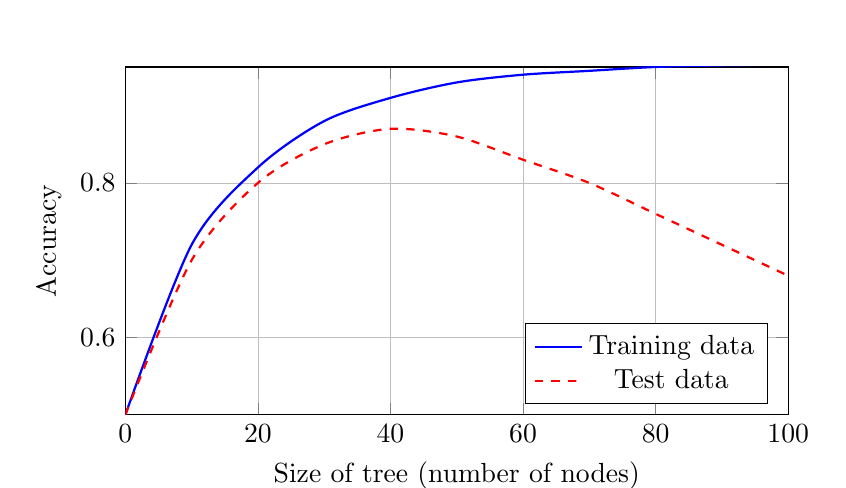
\begin{tikzpicture}
\begin{axis}[
    width=10cm,
    height=6cm,
    xlabel={Size of tree (number of nodes)},
    ylabel={Accuracy},
    xmin=0, xmax=100,
    ymin=0.5, ymax=0.95,
    legend pos=south east,
    grid=both,
    grid style={line width=.1pt, draw=gray!10},
    major grid style={line width=.2pt,draw=gray!50},
]

% Training data curve
\addplot[color=blue, thick, smooth] coordinates {
    (0,0.5) (10,0.72) (20,0.82) (30,0.88) (40,0.91) 
    (50,0.93) (60,0.94) (70,0.945) (80,0.95) (90,0.952) (100,0.953)
};

% Test data curve
\addplot[color=red, thick, dashed, smooth] coordinates {
    (0,0.5) (10,0.70) (20,0.80) (30,0.85) (40,0.87) 
    (50,0.86) (60,0.83) (70,0.80) (80,0.76) (90,0.72) (100,0.68)
};

\legend{Training data, Test data}
\end{axis}
\end{tikzpicture}
\end{center}

\textbf{Observations:}
\begin{itemize}
    \item Training accuracy continues to increase with tree size
    \item Test accuracy initially increases, then decreases
    \item The optimal tree size is around 30-40 nodes
    \item Larger trees overfit to the training data
\end{itemize}

\subsection{Techniques to Prevent Overfitting}

Standard machine learning techniques apply to decision trees:

\begin{enumerate}
    \item \textbf{Early stopping}: Stop growing the tree before it perfectly fits the training data
    \begin{itemize}
        \item Set a maximum depth
        \item Require a minimum number of samples to split
        \item Require a minimum information gain to split
    \end{itemize}
    
    \item \textbf{Pruning}: Build a full tree, then remove branches that don't improve validation performance
    
    \item \textbf{Regularization}: Add penalties for tree complexity
    
    \item \textbf{Data augmentation}: Increase training data
    
    \item \textbf{Ensemble methods}: Combine multiple trees (Random Forest, boosting)
\end{enumerate}

\subsection{Pruning (Post-processing)}

Pruning is a technique to reduce complexity \textit{after} tree building:

\begin{enumerate}
    \item \textbf{Build the full tree}: Grow the tree until each leaf node is pure or a stopping criterion is met
    
    \item \textbf{Evaluate nodes from bottom to top}: Starting from the bottom, evaluate each node to see if pruning it would improve performance on a validation set
    
    \item \textbf{Define cost-complexity measure}: Consider both the accuracy of the node and the size of the subtree rooted at that node
    
    \item \textbf{Prune nodes iteratively}: Identify the node with the smallest cost-complexity measure and prune its subtree (turn it into a leaf labeled with the majority class)
    
    \item \textbf{Repeat until done}: Continue until a suitable tree is achieved or further pruning doesn't improve performance
\end{enumerate}

\section{Decision Trees for Different Data Types}

\subsection{Continuous Attributes}

So far, we have focused on categorical attributes, but decision trees can also handle continuous attributes.

\textbf{Strategy:} Pick a threshold to create a binary split.

For example, for a continuous attribute like temperature:
\[
\phi(\text{temperature}) = \begin{cases}
L & \text{if temperature} > 77.8 \\
R & \text{else}
\end{cases}
\]

\textbf{How to choose the threshold?}
\begin{itemize}
    \item Consider all possible split points (or a sample of them)
    \item For each candidate threshold, compute the information gain (or Gini impurity reduction)
    \item Choose the threshold that maximizes information gain
\end{itemize}

\textbf{Geometric interpretation:}
\begin{itemize}
    \item Each split creates an axis-aligned boundary in feature space
    \item For 2D data with continuous features \(x_1\) and \(x_2\), splits create rectangular regions
    \item Example splits: \(x_1 > \theta_1\), \(x_2 < \theta_2\), \(x_2 > \theta_3\), \(x_1 < \theta_4\)
\end{itemize}

\subsection{Multi-class Classification}

Decision trees naturally extend to multi-class problems (\(k\) different classes):

\begin{itemize}
    \item At each leaf, predict the \textbf{most frequent class} in that subset
    
    \item Entropy for multi-class:
    \[
    H(S) = -\sum_{c=1}^{k} p(c) \log_2 p(c)
    \]
    Where \(p(c)\) is the proportion of examples of class \(c\) in subset \(S\)
    
    \item Information gain and Gini impurity formulas extend naturally to \(k\) classes
\end{itemize}

\section{Decision Trees: Summary}

\subsection{Advantages (Pros)}

\begin{itemize}
    \item \textbf{Interpretable}: Humans can understand the reason for decisions
    \item \textbf{Handles irrelevant data}: Irrelevant features have Gain = 0 and won't be selected
    \item \textbf{Handles missing data}: Can be adapted to deal with missing values
    \item \textbf{Very compact}: After pruning, \# nodes \(\ll\) \# training data
    \item \textbf{Fast at test time}: \(O(\text{depth})\), where depth \(\ll\) \# training data
    \item \textbf{No feature scaling needed}: Works with features on different scales
\end{itemize}

\subsection{Disadvantages (Cons)}

\begin{itemize}
    \item \textbf{Greedy algorithm}: May not find the globally optimal tree (locally optimal choices at each split)
    
    \item \textbf{NP-hard problem}: Finding the optimal tree is exponentially difficult (exponentially many possible trees)
    
    \item \textbf{Only axis-aligned splits}: Cannot naturally capture diagonal decision boundaries
    \begin{itemize}
        \item Linear classifiers can have diagonal boundaries
        \item Decision trees create rectangular partitions
        \item This limits expressiveness for some problems
    \end{itemize}
    
    \item \textbf{High variance}: Small changes in training data can lead to very different trees
    
    \item \textbf{Prone to overfitting}: Especially with deep trees
\end{itemize}

\subsection{Key Takeaways}

\begin{itemize}
    \item \textbf{ID3 algorithm}: Grows decision tree from root down, greedily selecting the next best attribute using information gain
    
    \item \textbf{Entropy}: Measures uncertainty (impurity) in a set
    
    \item \textbf{Information Gain}: Measures the reduction in uncertainty following a split
    
    \item \textbf{Complete hypothesis space}: Searches the entire space of possible trees
    
    \item \textbf{Preference}: Prefers smaller trees and high information gain at the root
    
    \item \textbf{Overfitting}: Addressed by post-pruning (remove nodes while accuracy increases on validation set)
    
    \item \textbf{Performance}: Fast, compact, and interpretable
\end{itemize}

\section{Random Forests}

Random forests address many limitations of individual decision trees by combining multiple trees into an ensemble.

\subsection{What is a Random Forest?}

\textbf{Random forests are ensembles of decision trees.}

\begin{itemize}
    \item Each tree is trained on a \textbf{bootstrapped version} of the training set (sampled with replacement)
    \item This creates diversity among the trees
    \item Different trees make different errors
    \item Combining their predictions reduces overall error
\end{itemize}

\subsubsection{Sampling with Replacement (Bootstrapping)}

Given a dataset \(\mathcal{D} = \{(\mathbf{x}_1, y_1), \ldots, (\mathbf{x}_n, y_n)\}\):

\begin{enumerate}
    \item For each tree \(t_i\), create a new dataset \(\mathcal{D}_i\) by:
    \begin{itemize}
        \item Randomly sampling \(n\) examples from \(\mathcal{D}\) \textbf{with replacement}
        \item Some examples may appear multiple times
        \item Some examples may not appear at all (approximately 37\% are left out)
    \end{itemize}
    
    \item Train tree \(t_i\) on dataset \(\mathcal{D}_i\)
    
    \item Repeat for all \(T\) trees in the forest
\end{enumerate}

\subsection{Random Feature Selection}

In addition to bootstrap sampling, random forests introduce randomness in feature selection:

\begin{itemize}
    \item At each node, instead of considering all features for splitting, only a \textbf{random subset} of features is considered
    
    \item Typical choices:
    \begin{itemize}
        \item For classification: \(\sqrt{d}\) features, where \(d\) is the total number of features
        \item For regression: \(d/3\) features
    \end{itemize}
    
    \item This helps to \textbf{decorrelate} decision trees
    
    \item \textbf{Extremely randomized trees} take this further by sampling split thresholds randomly instead of optimizing them
\end{itemize}

\subsection{Random Forest Prediction}

The final prediction of a random forest is obtained by \textbf{aggregating} the predictions of all trees:

\begin{tcolorbox}[colback=green!5!white,colframe=green!75!black,title=\textbf{Random Forest Prediction}]
\textbf{For classification:}
\[
\hat{y}_{\text{RF}}(\mathbf{x}) = \text{mode}\{f_{t_1}(\mathbf{x}), \ldots, f_{t_T}(\mathbf{x})\}
\]
(Majority vote across all trees)

\textbf{For regression:}
\[
\hat{y}_{\text{RF}}(\mathbf{x}) = \frac{1}{T} \sum_{i=1}^{T} f_{t_i}(\mathbf{x})
\]
(Average of all tree predictions)
\end{tcolorbox}

\subsection{Why Random Forests Work}

Random forests work well because of several key principles:

\begin{enumerate}
    \item \textbf{Variance reduction}: Averaging multiple models reduces variance without increasing bias
    
    \item \textbf{Decorrelation}: Random feature selection ensures trees make different types of errors
    
    \item \textbf{Robustness}: Errors of individual trees tend to cancel out
    
    \item \textbf{Overfitting resistance}: Individual trees may overfit, but the ensemble typically does not
\end{enumerate}

\textbf{Bias-Variance Trade-off:}
\begin{itemize}
    \item Individual deep trees have low bias but high variance
    \item Averaging many trees keeps bias low while reducing variance
    \item Result: Better generalization performance
\end{itemize}

\section{Ensemble Methods}

Random forests are one example of a broader class of techniques called \textbf{ensemble methods}.

\subsection{What are Ensemble Methods?}

\textbf{Ensemble learning} combines different models to obtain more accurate predictions than any individual model.

\begin{tcolorbox}[colback=blue!5!white,colframe=blue!75!black,title=\textbf{Ensemble Learning Principle}]
``Wisdom of crowds'': Aggregating predictions from multiple models often yields better performance than using a single model.
\end{tcolorbox}

\subsection{Types of Ensemble Methods}

There are three main types of ensemble methods:

\begin{enumerate}
    \item \textbf{Bagging} (Bootstrap Aggregating)
    \item \textbf{Boosting}
    \item \textbf{Stacking}
\end{enumerate}

\section{Bagging (Bootstrap Aggregating)}

\subsection{The Bagging Algorithm}

Bagging is a technique where we train \(T\) models on \(T\) different samplings of the dataset.

\textbf{Procedure:}
\begin{enumerate}
    \item Take the original dataset \(\mathcal{D}\)
    
    \item Create \(T\) bootstrap samples:
    \begin{itemize}
        \item \(\mathcal{D}_1\): Sample \(n\) examples from \(\mathcal{D}\) with replacement
        \item \(\mathcal{D}_2\): Sample \(n\) examples from \(\mathcal{D}\) with replacement
        \item ...
        \item \(\mathcal{D}_T\): Sample \(n\) examples from \(\mathcal{D}\) with replacement
    \end{itemize}
    
    \item Train a model on each bootstrap sample:
    \begin{itemize}
        \item Model 1 trained on \(\mathcal{D}_1\)
        \item Model 2 trained on \(\mathcal{D}_2\)
        \item ...
        \item Model \(T\) trained on \(\mathcal{D}_T\)
    \end{itemize}
    
    \item \textbf{Aggregate} predictions:
    \begin{itemize}
        \item Classification: Majority vote
        \item Regression: Average
    \end{itemize}
\end{enumerate}

\subsection{Benefits of Bagging}

\begin{itemize}
    \item \textbf{Reduces variance}: Different bootstrap samples lead to different models; averaging reduces variance
    
    \item \textbf{Doesn't increase bias}: Each model is trained on a dataset of the same size as the original
    
    \item \textbf{Robust to overfitting}: Individual models may overfit to their bootstrap samples, but averaging helps
    
    \item \textbf{Parallel training}: All models can be trained independently and in parallel
\end{itemize}

\subsection{When to Use Bagging}

Bagging works best with:
\begin{itemize}
    \item \textbf{High-variance, low-bias models}: e.g., deep decision trees
    \item Models that are sensitive to small changes in training data
    \item Situations where you want to reduce overfitting
\end{itemize}

\section{Boosting}

Boosting is a different ensemble strategy that trains models \textbf{sequentially}, with each new model focusing on the errors of previous models.

\subsection{Key Differences from Bagging}

\begin{center}
\begin{tabular}{|l|l|l|}
\hline
\textbf{Aspect} & \textbf{Bagging} & \textbf{Boosting} \\
\hline
Training & Parallel (independent) & Sequential (dependent) \\
\hline
Sampling & Uniform (with replacement) & Weighted (focus on errors) \\
\hline
Model weights & Equal & Based on performance \\
\hline
Goal & Reduce variance & Reduce bias and variance \\
\hline
\end{tabular}
\end{center}

\subsection{Boosting Intuition}

\begin{itemize}
    \item Trained models are \textbf{weighted based on their performance}
    
    \item Weak classifiers are learned \textbf{sequentially}
    
    \item The more mistakes the previous classifier makes on a dataset, the more those misclassified examples are \textbf{weighted for the next classifier}
    
    \item Each new model focuses on the ``hard'' examples that previous models got wrong
\end{itemize}

\subsection{Weak Learners}

Ensemble methods often use \textbf{weak learners} rather than complex models.

\begin{definition}[Weak Learner]
A weak learner is a classification model that performs \textbf{slightly better than random guessing}.

For binary classification with balanced classes:
\begin{itemize}
    \item Random guessing: 50\% accuracy
    \item Weak learner: slightly better than 50\% (e.g., 55\%)
\end{itemize}
\end{definition}

\textbf{Examples of weak learners:}
\begin{itemize}
    \item \textbf{Decision stump}: A decision tree with only one split (depth = 1)
    \item \textbf{1-Nearest Neighbor}: k-NN with k=1 on a subset of features
    \item Simple linear classifiers on a single feature
\end{itemize}

\textbf{Why use weak learners?}
\begin{itemize}
    \item Fast to train
    \item Less likely to overfit individually
    \item Ensemble of many weak learners can create a strong classifier
    \item ``Two heads are better than one'' principle
\end{itemize}

\subsection{AdaBoost (Adaptive Boosting)}

AdaBoost is one of the most popular boosting algorithms.

\begin{tcolorbox}[colback=orange!5!white,colframe=orange!75!black,title=\textbf{AdaBoost Algorithm}]
\textbf{Step 1:} Initialize weights uniformly for all training samples:
\[
w_i^{(1)} = \frac{1}{n} \quad \text{for } i = 1, \ldots, n
\]

\textbf{Step 2:} For \(t = 1\) to \(T\):
\begin{enumerate}
    \item Train a weak classifier \(h_t\) using the current weights \(w^{(t)}\)
    
    \item Compute the weighted error:
    \[
    \epsilon_t = \sum_{i: h_t(\mathbf{x}_i) \neq y_i} w_i^{(t)}
    \]
    
    \item Compute classifier weight:
    \[
    \alpha_t = \frac{1}{2} \ln\left(\frac{1 - \epsilon_t}{\epsilon_t}\right)
    \]
    
    \item Update sample weights:
    \[
    w_i^{(t+1)} = w_i^{(t)} \cdot \exp\left(-\alpha_t y_i h_t(\mathbf{x}_i)\right)
    \]
    (Increase weight for misclassified samples, decrease for correctly classified)
    
    \item Normalize weights: \(w^{(t+1)} \leftarrow w^{(t+1)} / \sum_i w_i^{(t+1)}\)
\end{enumerate}

\textbf{Step 3:} Final classifier:
\[
H(\mathbf{x}) = \text{sign}\left(\sum_{t=1}^{T} \alpha_t h_t(\mathbf{x})\right)
\]
(Weighted vote of all weak classifiers)
\end{tcolorbox}

\subsection{AdaBoost: Key Steps Explained}

\textbf{Step 1: Initialize with equal weights}
\begin{itemize}
    \item All training samples start with equal importance
    \item Build the first weak classifier on this uniformly weighted dataset
    \item Check which samples are correctly classified and which are not
\end{itemize}

\textbf{Step 2: Increase weights for misclassified samples}
\begin{itemize}
    \item Samples that were misclassified get higher weights
    \item This makes classifying them correctly more important for the next model
    \item The next weak classifier will focus more on these "hard" examples
\end{itemize}

\textbf{Step 3: Iterate until convergence}
\begin{itemize}
    \item Repeat until all data points are correctly classified
    \item OR until a maximum number of iterations is reached
    \item Each iteration focuses on the remaining difficult examples
\end{itemize}

\subsection{AdaBoost Properties}

\begin{itemize}
    \item \textbf{Adaptive}: Adapts to the errors of previous weak learners
    
    \item \textbf{Reduces bias and variance}: Combines weak learners to create a strong learner
    
    \item \textbf{Sensitive to noisy data}: Can overfit if there are many outliers (keeps increasing their weights)
    
    \item \textbf{No need for feature selection}: Weak learners can be based on individual features
    
    \item \textbf{Fast training}: Each weak learner is simple and fast to train
\end{itemize}

\section{Stacking}

Stacking (stacked generalization) is a more sophisticated ensemble method that uses a \textbf{meta-model} to combine base models.

\subsection{What is Stacking?}

Stacking combines predictions of multiple ML models (called \textbf{base models}) to improve overall performance.

\textbf{Key differences from bagging and boosting:}
\begin{itemize}
    \item Base models are typically \textbf{heterogeneous} (different types of models)
    \item Uses a \textbf{meta-model} to learn how to combine base model predictions
    \item Can be used for both regression and classification
    \item Often more powerful than bagging or boosting alone
\end{itemize}

\subsection{The Stacking Process}

\begin{tcolorbox}[colback=purple!5!white,colframe=purple!75!black,title=\textbf{Stacking Algorithm}]
\textbf{Level 0 (Base Models):}
\begin{enumerate}
    \item Train multiple diverse base models on the training set:
    \begin{itemize}
        \item Model 1: e.g., Decision Tree
        \item Model 2: e.g., Logistic Regression
        \item Model 3: e.g., Support Vector Machine
        \item Model 4: e.g., Neural Network
    \end{itemize}
    
    \item Generate predictions from each base model on the training set
\end{enumerate}

\textbf{Level 1 (Meta-Model):}
\begin{enumerate}
    \item Use the predictions from base models as \textbf{features}
    
    \item Train a \textbf{meta-model} that learns how to combine these predictions
    
    \item The meta-model learns which base models to trust for which types of inputs
\end{enumerate}

\textbf{Prediction:}
\begin{enumerate}
    \item For a new input \(\mathbf{x}\):
    \begin{itemize}
        \item Get predictions from all base models
        \item Feed these predictions to the meta-model
        \item Meta-model outputs the final prediction
    \end{itemize}
\end{enumerate}
\end{tcolorbox}

\subsection{Why Stacking Works}

\begin{itemize}
    \item \textbf{Diversity}: Different models capture different patterns in the data
    
    \item \textbf{Complementary strengths}: Each model may excel in different regions of the input space
    
    \item \textbf{Learned combination}: The meta-model learns the optimal way to combine predictions (better than simple averaging)
    
    \item \textbf{Flexibility}: Can combine any types of models
\end{itemize}

\subsection{Stacking Best Practices}

\begin{itemize}
    \item \textbf{Use diverse base models}: Different model types, different hyperparameters
    
    \item \textbf{Avoid data leakage}: Use cross-validation to generate training predictions for the meta-model
    
    \item \textbf{Keep meta-model simple}: Often a simple linear model or logistic regression works well
    
    \item \textbf{Regularization}: Add regularization to prevent the meta-model from overfitting
\end{itemize}

\subsection{Comparison of Ensemble Methods}

\begin{center}
\small
\begin{tabular}{|p{2.5cm}|p{3.5cm}|p{3.5cm}|p{3.5cm}|}
\hline
\textbf{Method} & \textbf{Base Models} & \textbf{Training} & \textbf{Combination} \\
\hline
\textbf{Bagging} & Same type (homogeneous), trained on bootstrap samples & Parallel, independent & Equal weight voting/averaging \\
\hline
\textbf{Boosting} & Same type (weak learners), trained sequentially & Sequential, each focuses on previous errors & Weighted voting based on model performance \\
\hline
\textbf{Stacking} & Different types (heterogeneous) & Parallel for base models, then meta-model & Meta-model learns optimal combination \\
\hline
\end{tabular}
\end{center}

\subsection{Key Takeaways}

\begin{tcolorbox}[colback=green!5!white,colframe=green!75!black,title=\textbf{Main Lessons}]
\begin{enumerate}
    \item \textbf{Single models vs. Ensembles}: Ensembles generally outperform single models
    
    \item \textbf{Bias-Variance tradeoff}: Different ensemble methods address different aspects
    \begin{itemize}
        \item Bagging reduces variance
        \item Boosting reduces both bias and variance
        \item Stacking leverages diverse model strengths
    \end{itemize}
    
    \item \textbf{Interpretability vs. Performance}: Trade-off between understanding and accuracy
    
    \item \textbf{Computational cost}: Ensembles are slower to train and predict than single models
    
    \item \textbf{Real-world impact}: Random forests and boosting (e.g., XGBoost, LightGBM) are among the most successful ML methods in practice
\end{enumerate}
\end{tcolorbox}


\newpage 

\part{Linear Discriminant Functions and Classification Methods}

\section{Linear Discriminant Functions}

The objective of this lecture is to present methods for learning \textbf{linear discriminant} functions of the form:
\[
g(x) = w^T x + w_0 \Leftrightarrow 
\begin{cases}
g(x) > 0 & x \in \omega_1 \\
g(x) < 0 & x \in \omega_2
\end{cases}
\]

where:
\begin{itemize}
    \item $w$ is the \textbf{weight vector}
    \item $w_0$ is the \textbf{threshold weight} or \textbf{bias}
    \item $\mathbf{x} = [x_1, \ldots, x_n]$, $\mathbf{w} = [w_1, \ldots, w_n]$
\end{itemize}

For a problem with 2 classes, the goal is to create a \textbf{linear function} $g(x)$ that separates the examples belonging to the two classes.

\textbf{Note:} $g(x) = 0 \Rightarrow$ either class

\begin{center}
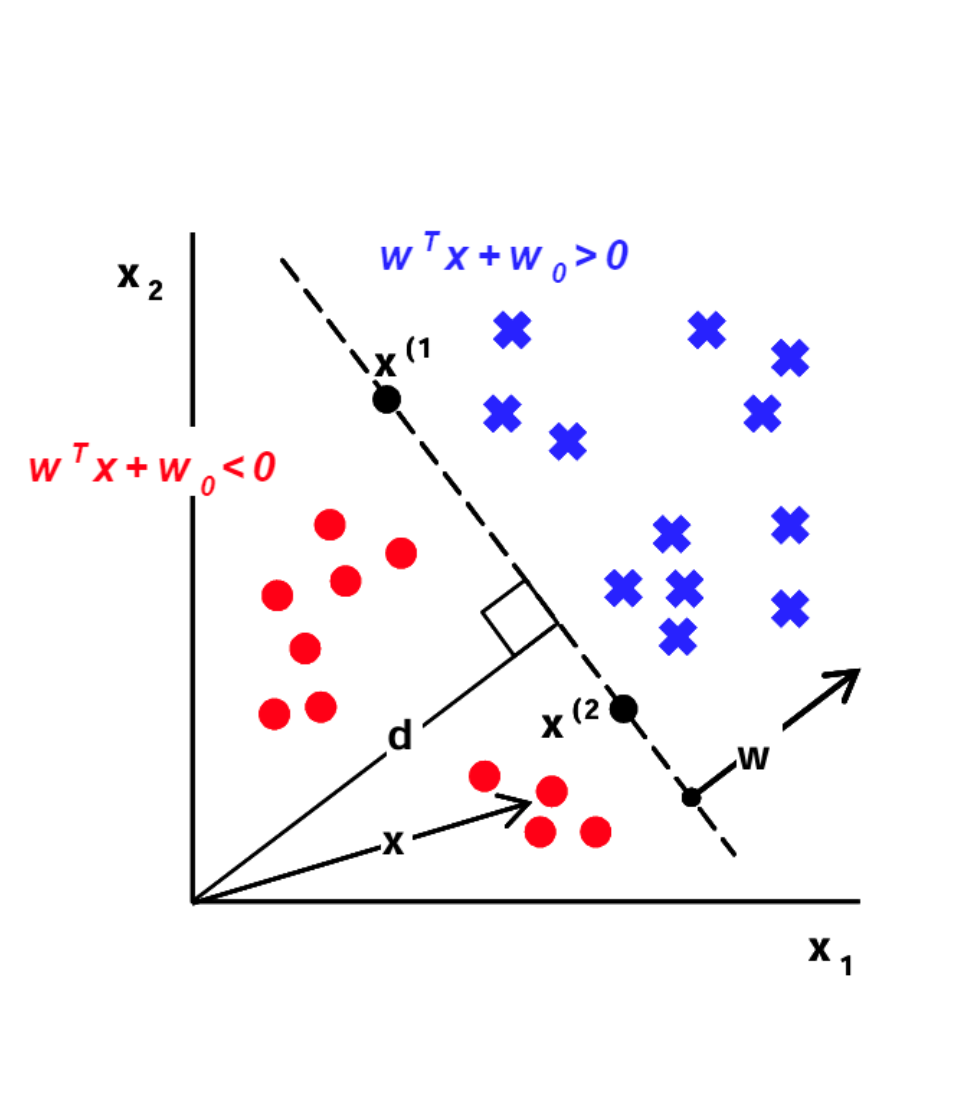
\includegraphics[width=0.5\textwidth]{figures/linear_discriminant_intro.png}
\end{center}

\subsection{Learning the Linear Discriminant Function}

Suppose we have a set of $m$ samples $\mathbf{x}_1, \ldots, \mathbf{x}_m$, some tagged $\omega_1$ and others tagged $\omega_2$.

We want to use these samples to determine the weights $\mathbf{w}$ and $w_0$ of the linear discriminating function.

Suppose also that there is a solution for which the probability of error is very low.

Thus, a reasonable approach is to look for a weight vector that classifies all of the samples correctly or that the probability of making a mistake is zero.

If such a \textbf{weight vector} exists, the samples are said to be \textbf{linearly separable}.

\begin{center}
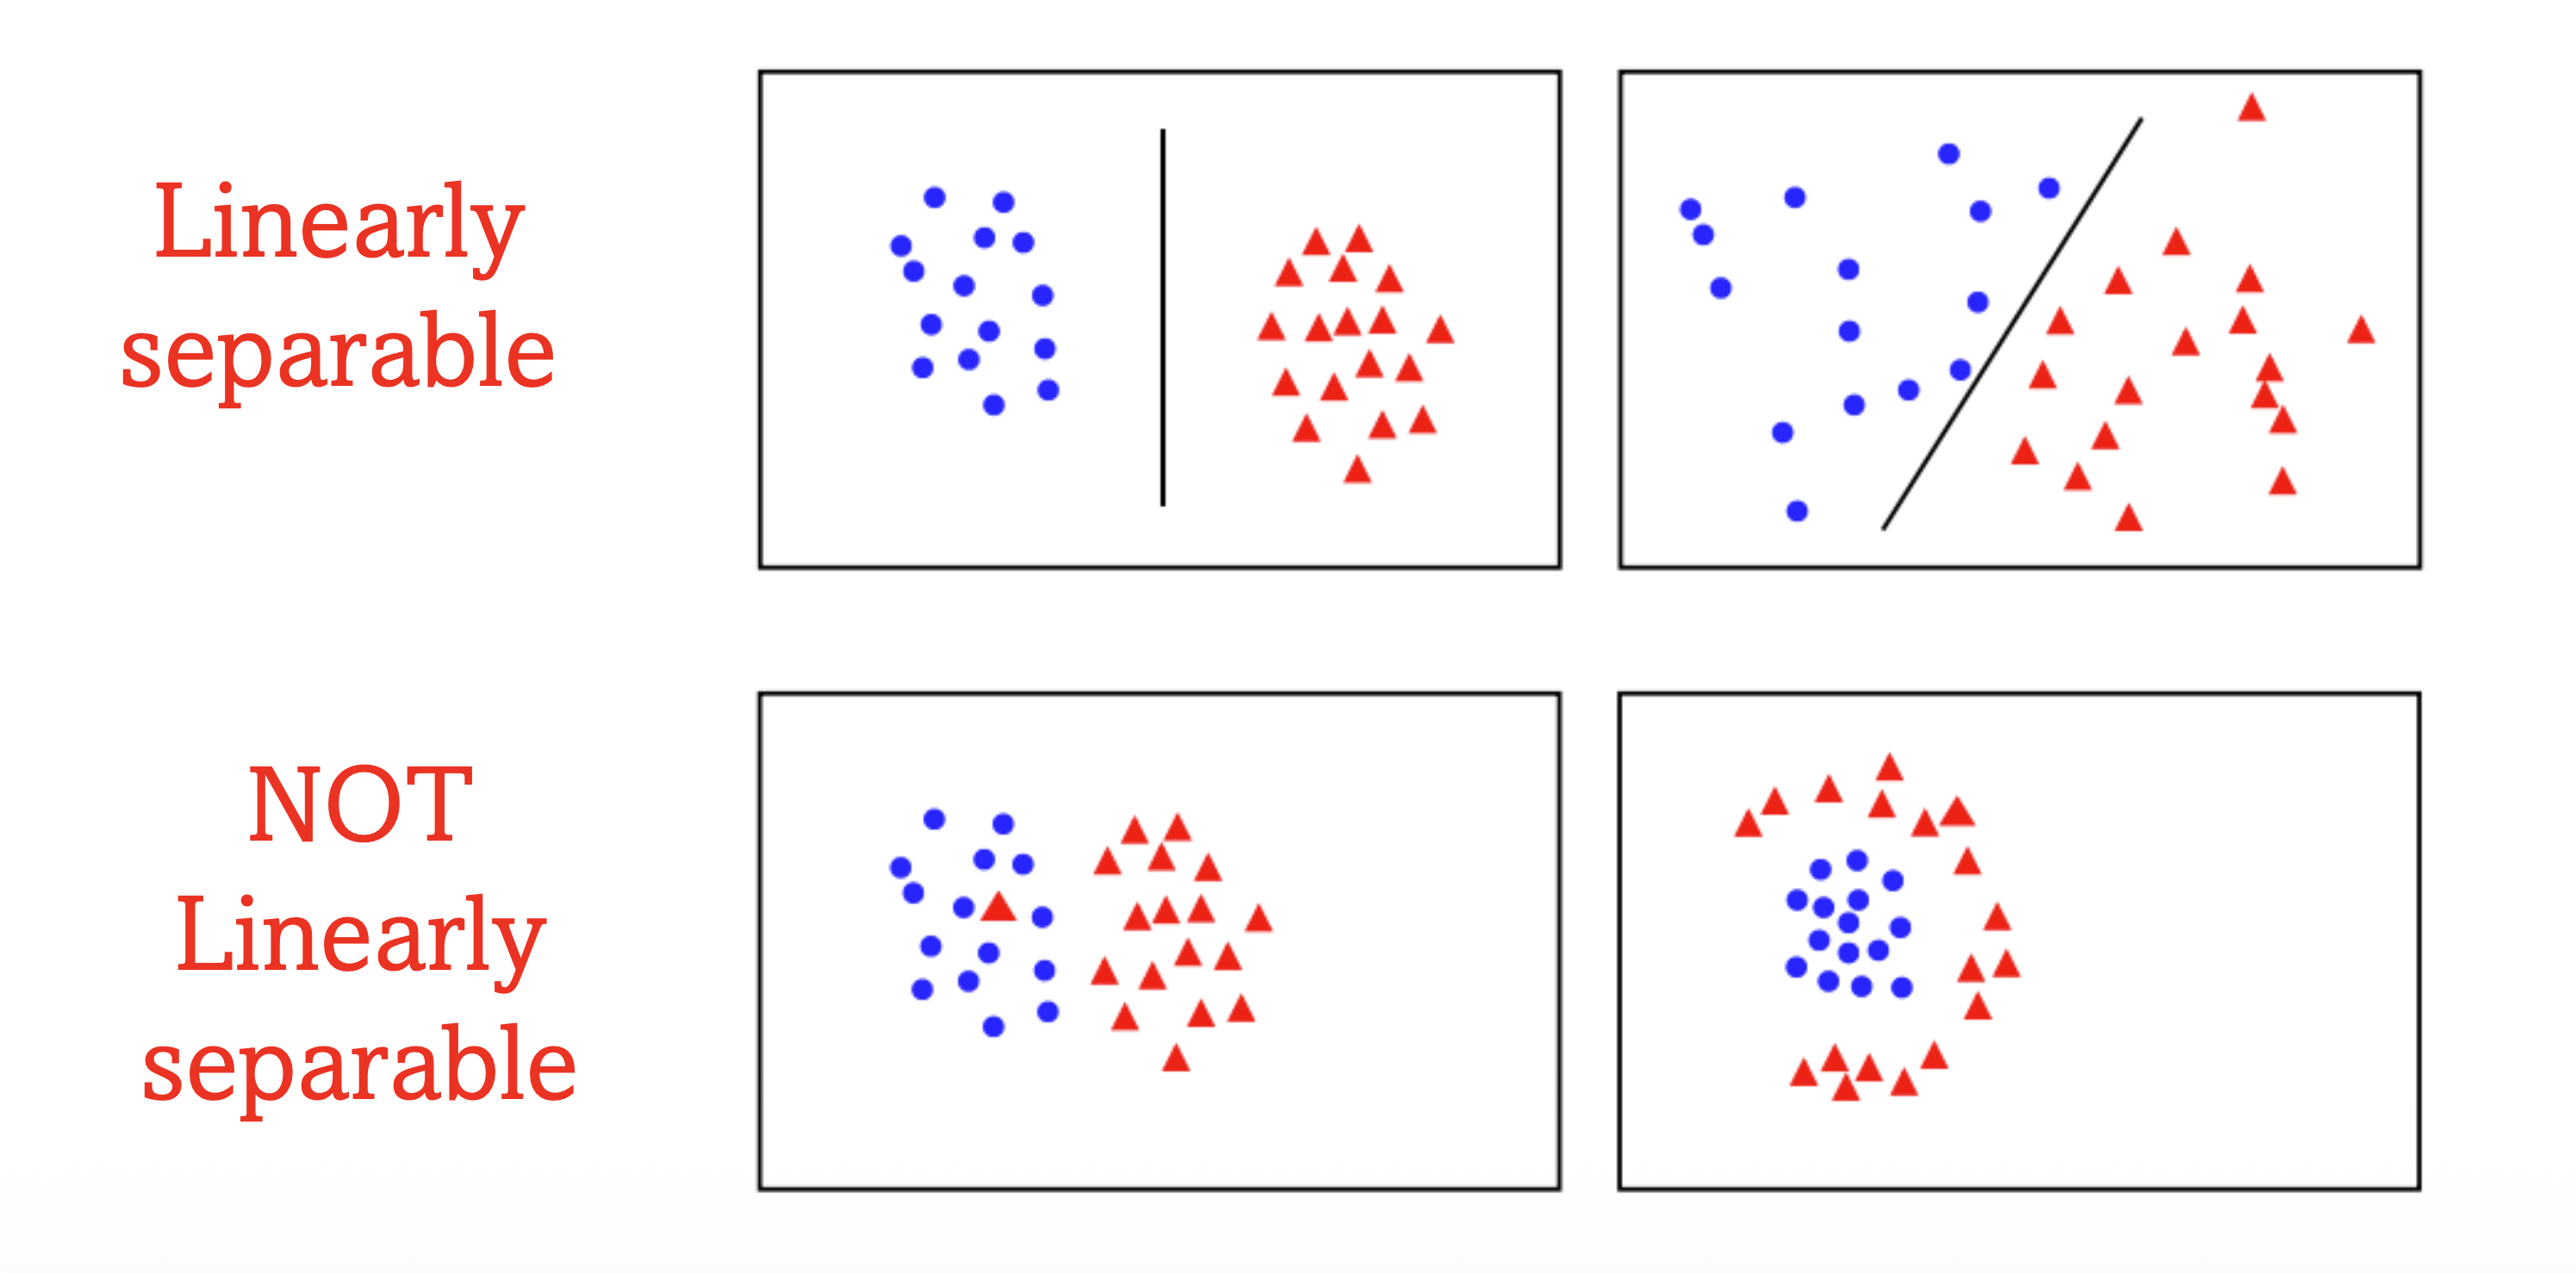
\includegraphics[width=0.5\textwidth]{figures/linear_discriminant_samples.png}
\end{center}

\subsection{Linear Separability}

Data are \textbf{linearly separable} if there exists a linear boundary (hyperplane) that perfectly separates the two classes.

\textbf{Examples:}
\begin{itemize}
    \item \textbf{Linearly separable}: Classes that can be separated by a straight line (in 2D) or hyperplane (in higher dimensions)
    \item \textbf{NOT Linearly separable}: Classes that cannot be separated by any linear boundary
\end{itemize}

\begin{center}
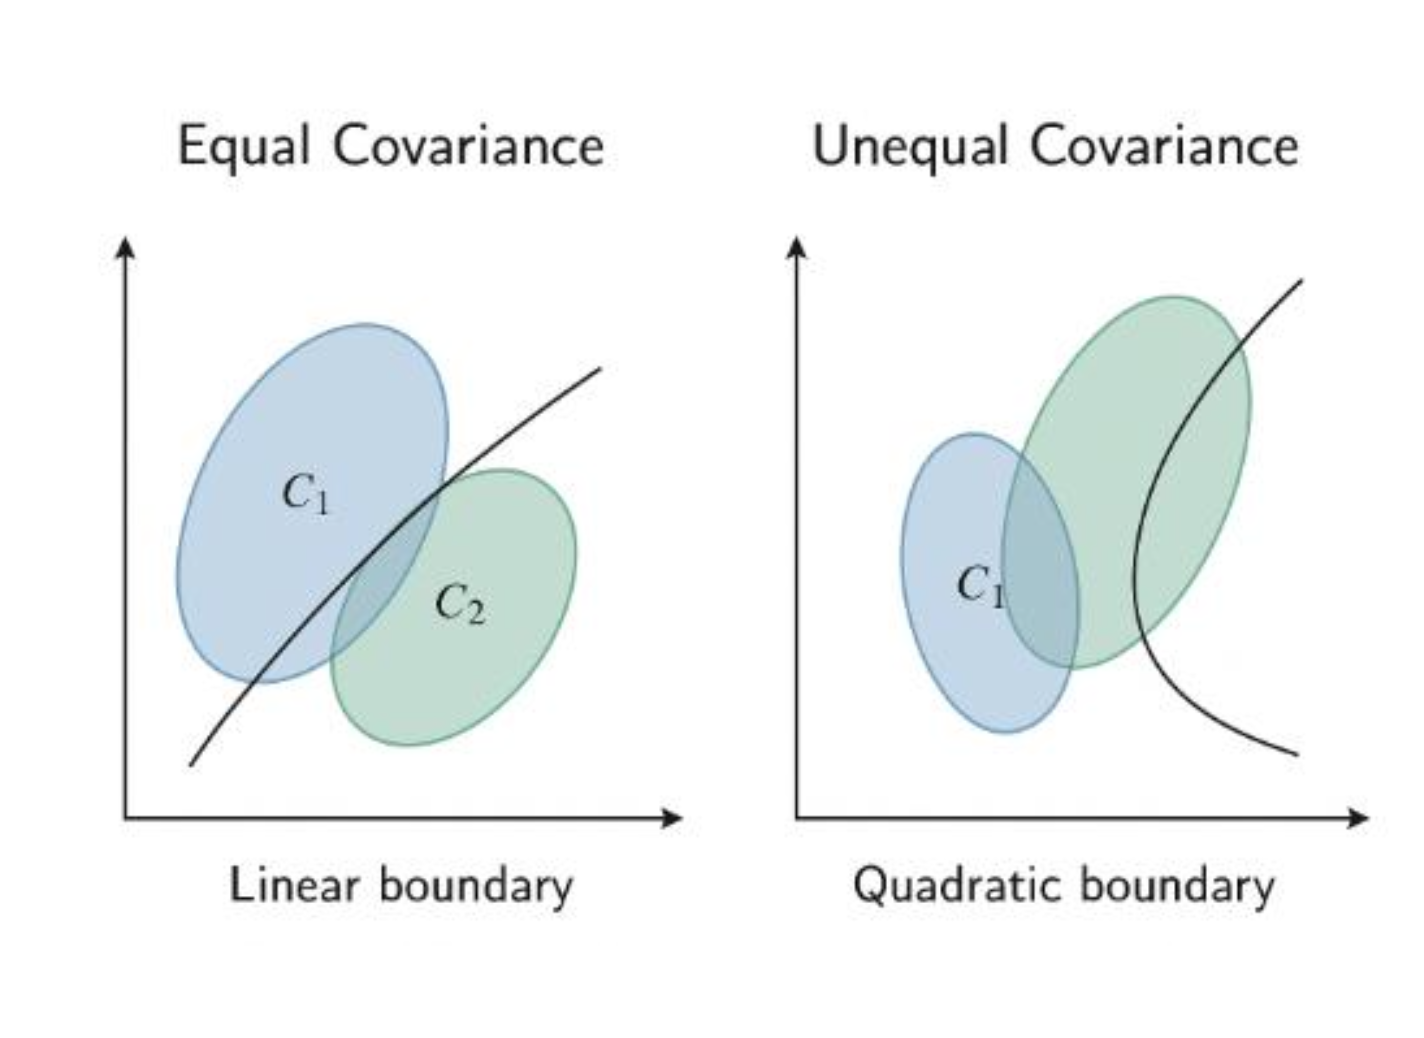
\includegraphics[width=0.6\textwidth]{figures/linear_separability_examples.png}
\end{center}

\subsection{Properties of Linear Discriminant Functions}

Linear discriminant functions are:
\begin{itemize}
    \item \textbf{Optimal for Gaussian distributions with equal covariance}: When the data follows Gaussian distributions with equal covariance matrices, the optimal decision boundary is linear
    
    \item \textbf{May not be optimal for other data distributions}, but they are very simple to use
    
    \item \textbf{Knowledge of class densities is not required} when using linear discriminant functions
    \begin{itemize}
        \item Therefore, we can say that this is a \textbf{non-parametric approach}
    \end{itemize}
\end{itemize}

\textbf{Note:} With unequal covariance, the optimal decision boundary is quadratic rather than linear.

\begin{center}
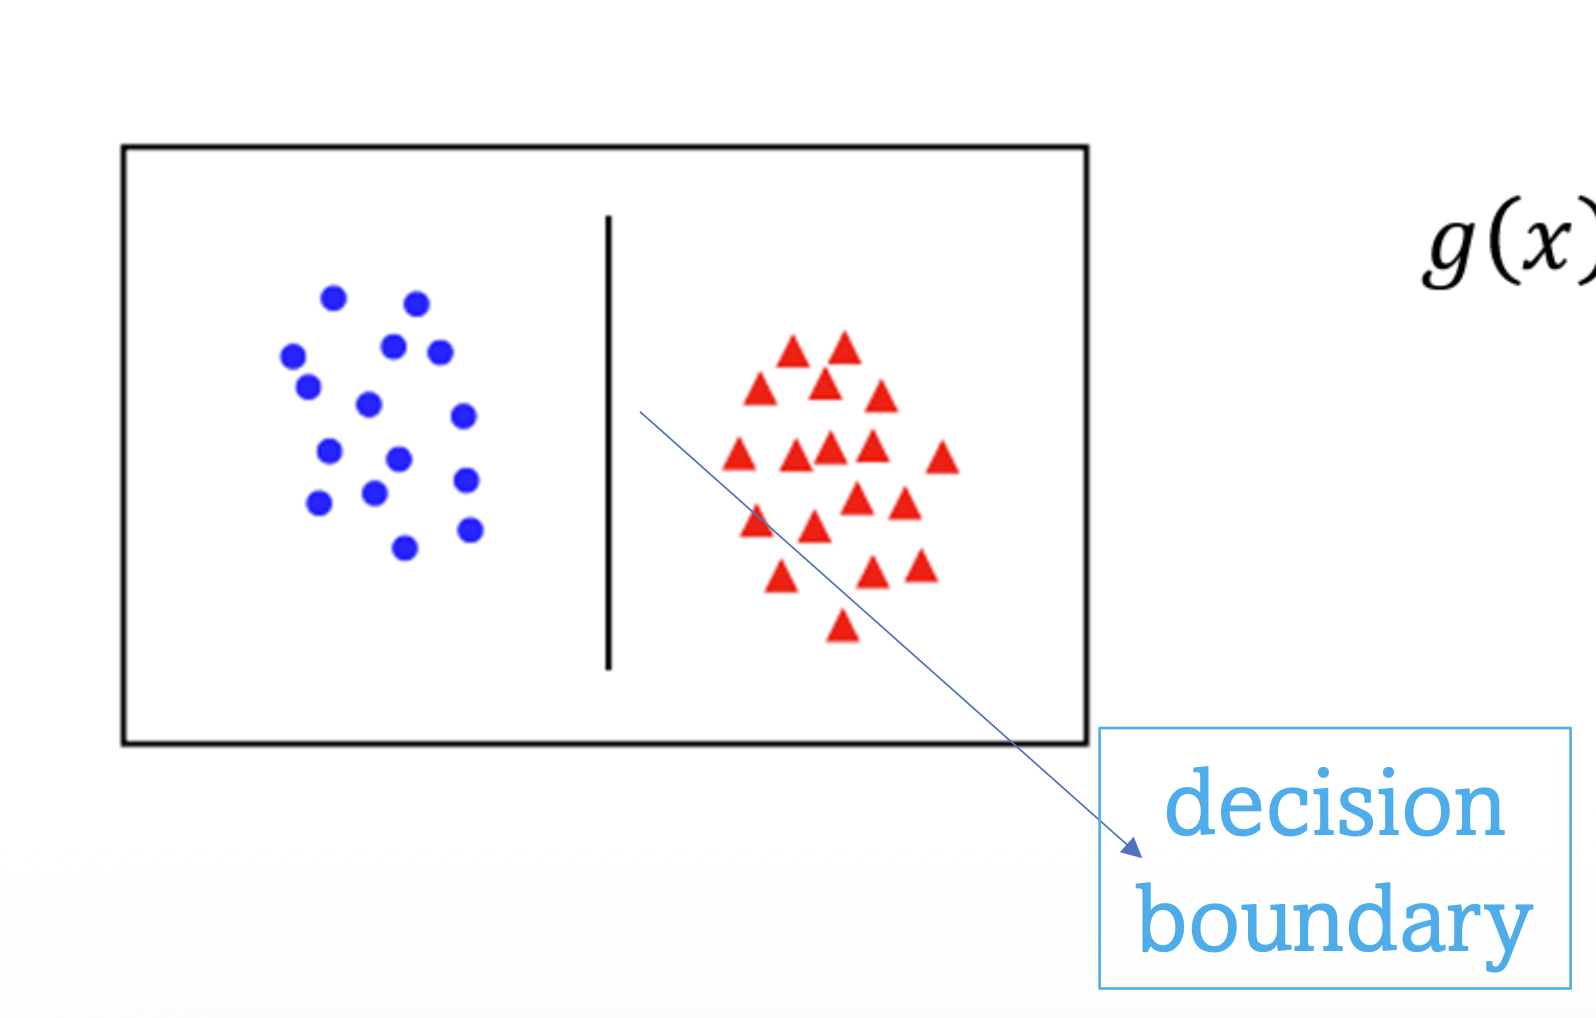
\includegraphics[width=0.6\textwidth]{figures/linear_discriminant_gaussian.png}
\end{center}

\section{Linear Classifiers}

Every linear discriminant function defines a linear classifier.

But not every linear classifier is necessarily described in the form of a "discriminant function" (although in practice, the terms are often used interchangeably).

\subsection{Decision Boundary}

The linear discriminant function is defined as:
\[
g(x) = w^T x + w_0 \Leftrightarrow 
\begin{cases}
g(x) > 0 & x \in \omega_1 \\
g(x) < 0 & x \in \omega_2
\end{cases}
\]

The \textbf{decision boundary} is defined by $g(x) = w^T x + w_0 = 0$:
\begin{itemize}
    \item In 2D, is a \textbf{line}
    \item In 3D, is a \textbf{plane}
    \item In nD, is a \textbf{hyperplane}
\end{itemize}

\begin{center}
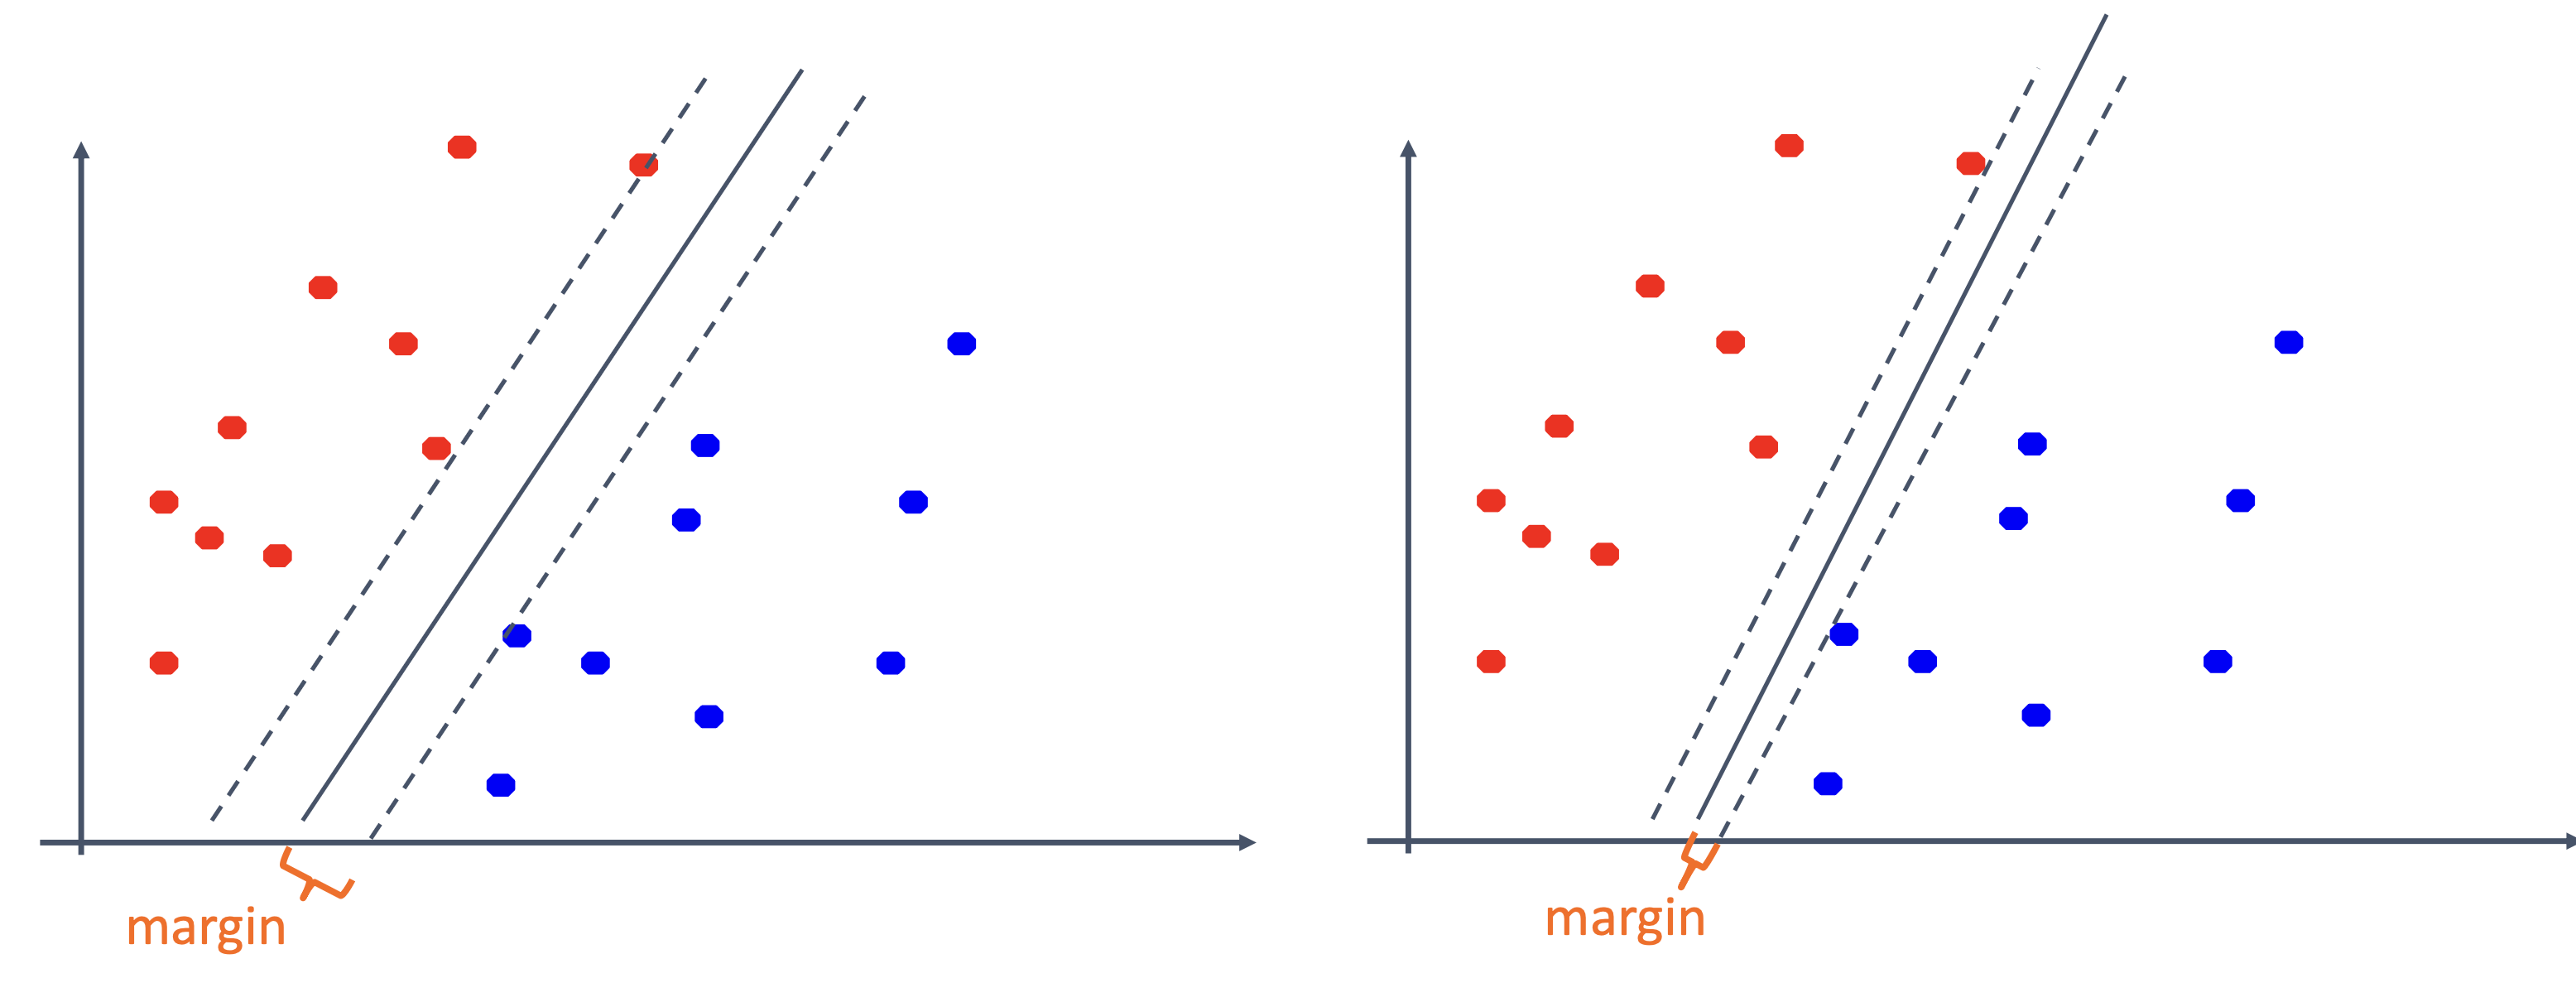
\includegraphics[width=0.5\textwidth]{figures/linear_classifiers_decision_boundary.png}
\end{center}

\subsection{The Role of Weights}

The training data is used to learn $\mathbf{w}$.

\textbf{Important:} Only $\mathbf{w}$ is needed to classify the new data point.

The equation $\mathbf{w}^{\mathrm{T}} \mathbf{x}_i = 0$ defines a hyperplane passing through the origin of the feature space, having $\mathbf{w}$ as a normal vector.

\begin{itemize}
    \item $\mathbf{w}$ determines the orientation of the decision hyperplane
    \item $w_0$ determines the location of the decision surface
\end{itemize}

\begin{center}
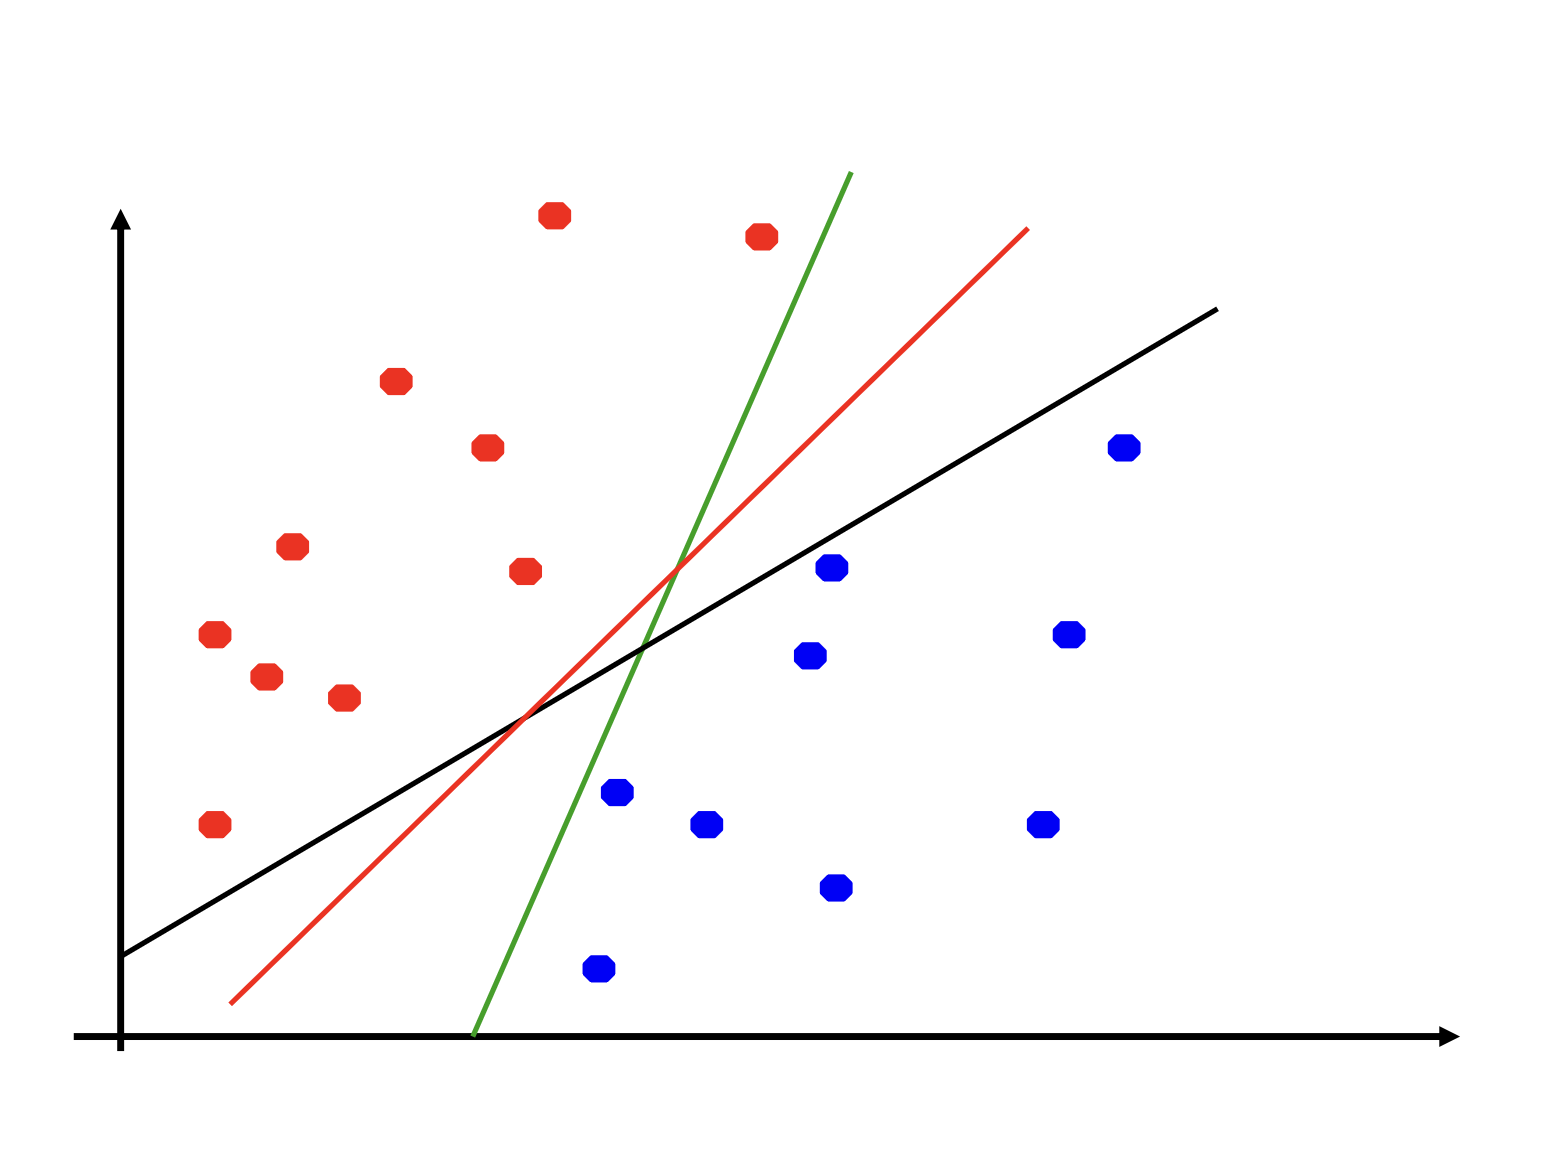
\includegraphics[width=0.5\textwidth]{figures/linear_classifiers_hyperplane.png}
\end{center}

\subsection{Which Hyperplanes?}

If a solution vector exists (if there is a hyperplane) then:
\begin{itemize}
    \item Which hyperplane a linear classifier choose when the data is linearly separable?
    \item The solution vector is not unique!
\end{itemize}

\begin{center}
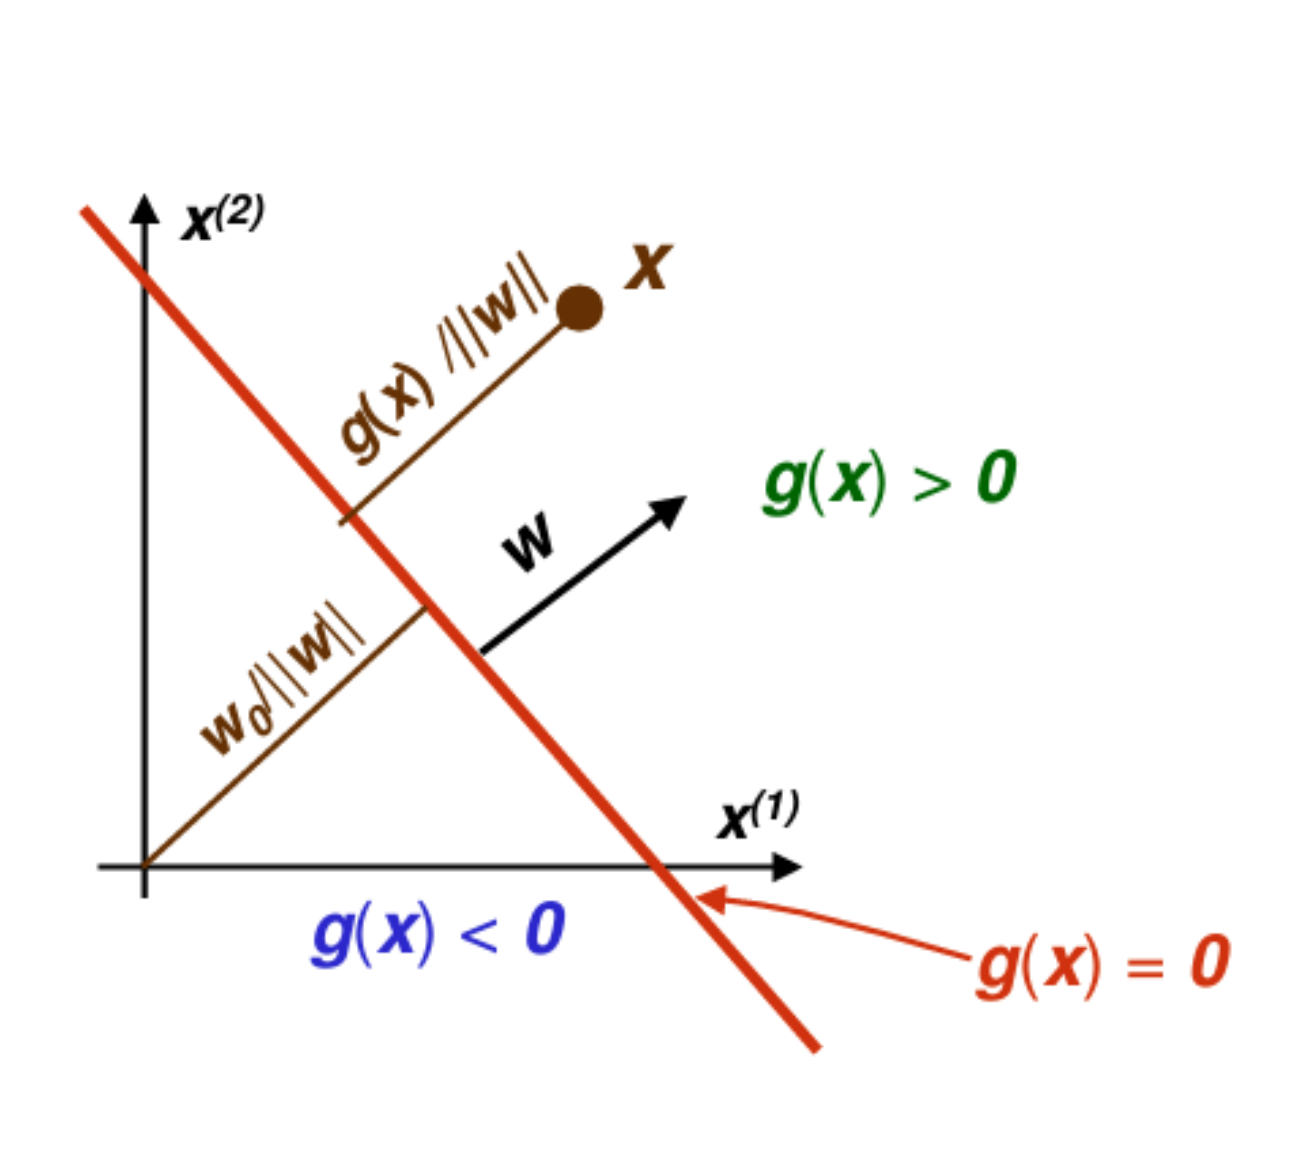
\includegraphics[width=0.5\textwidth]{figures/which_hyperplanes.png}
\end{center}

\subsection{Optimization Approaches}

There are different approaches to find the optimal weight vector:

\subsubsection{Unit-Length Weight Vector}

One possibility is to seek a \textbf{unit-length weight vector} that maximizes the minimum distance from the samples to the separating plane.

\subsubsection{Minimum-Length Weight Vector}

Another possibility is to seek the \textbf{minimum-length weight vector} satisfying:
\[
\mathbf{w}^{\mathrm{T}} \mathbf{x}_i \geq b, \quad \forall i
\]

where $b$ is a positive constant called the \textbf{margin}.

These techniques attempt to find a solution vector closer to the "middle" of the solution region:
\begin{itemize}
    \item In this way, the resulting solution is more likely to classify new test samples correctly
\end{itemize}

\subsection{The Margin}

\begin{definition}[Margin]
The \textbf{margin} of a classifier is the distance to the closest points of either class.
\end{definition}

A larger margin generally leads to better generalization performance on unseen data.

\section{Multi-Class Problems}

In case of a multi-class (C-class) problem:

\begin{tcolorbox}[colback=purple!5!white,colframe=purple!75!black,title=\textbf{Multi-Class Classification Strategies}]
\subsection*{One-vs-Rest Classifiers}
C-1 classifiers $g_i(\mathbf{x})$ are constructed, one for each class $C_i$ versus non-$C_i$.

\subsection*{One-vs-One Classifiers}
$C(C-1)/2$ binary classifiers (one-vs-one), and then classify a test sample following a \textbf{majority voting}.

\subsection*{Ambiguity Regions}
Both approaches lead to areas of \textbf{ambiguity}.
\end{tcolorbox}

\begin{center}
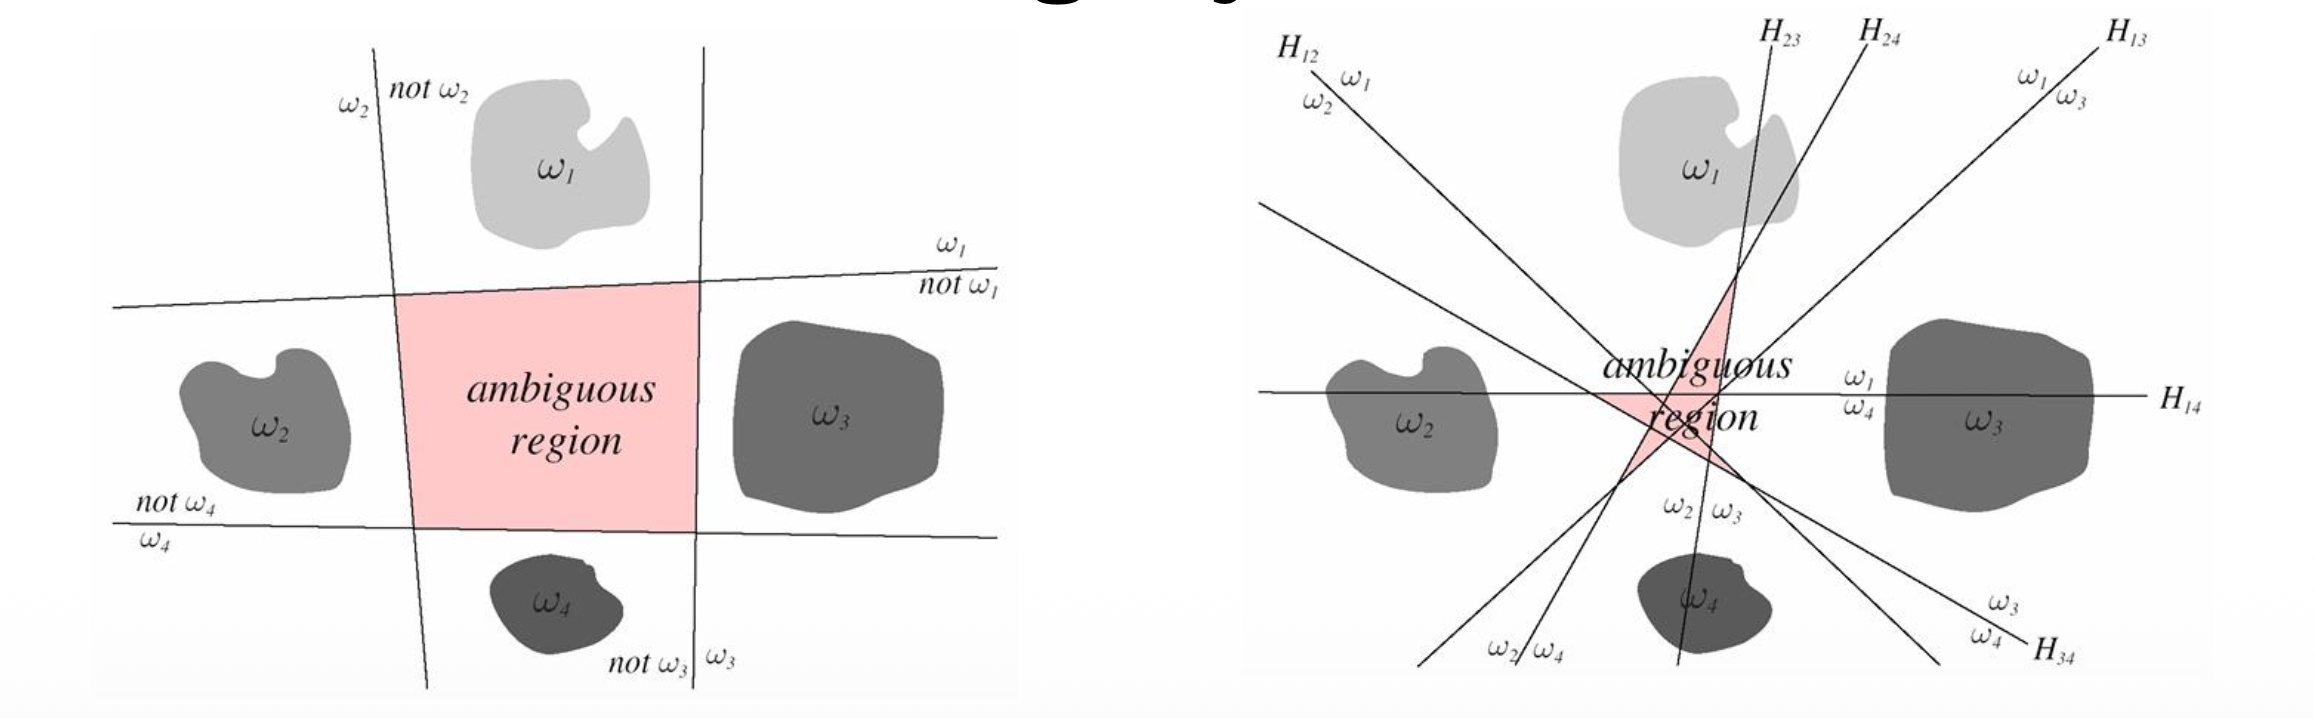
\includegraphics[width=0.6\textwidth]{figures/multiclass_ambiguity.png}
\end{center}

\section{LDF: Augmented Feature Vector}

LDF: $g(x) = w^T x + w_0$

\begin{tcolorbox}[colback=cyan!5!white,colframe=cyan!75!black,title=\textbf{Augmented Feature Vector Transformation}]
We can write it as:
\[
g(\mathbf{x}) = [w_0 \quad w^T] \begin{bmatrix} 1 \\ \mathbf{x} \end{bmatrix} = \mathbf{a}^T \mathbf{y} = g(\mathbf{y})
\]

where:
\begin{itemize}
    \item $\mathbf{a}$ is the \textbf{new weight vector}
    \item $\mathbf{y}$ is the \textbf{new feature vector} (called the \textbf{augmented feature vector})
\end{itemize}

We added a dummy dimension to get a completely equivalent new \textbf{homogeneous} problem.

\textbf{Old problem:} $g(\mathbf{x}) = w^t \mathbf{x} + w_0$, with $\mathbf{x} = [x_1, \ldots, x_d]$

\textbf{New problem:} $g(\mathbf{y}) = \mathbf{a}^T \mathbf{y}$, with $\mathbf{y} = [1, x_1, \ldots, x_d]$
\end{tcolorbox}

\textbf{Feature augmenting is done only for simpler notation.}

\textbf{Note:} Throughout these lecture notes we replace $\mathbf{a}$ with $\mathbf{w}$ for simplicity, since they both refer to weights.

\section{LDF: Training Error}

For the rest of the lecture, assume we have 2 classes.

We will use samples (training data) to determine weights $\mathbf{a}$ (or indicated with $\mathbf{w}$) in the discriminant function $g(\mathbf{y}) = \mathbf{a}^T \mathbf{y}$.

\subsection{Criterion for Determining Weights}

What should be our criterion for determining $\mathbf{a}$?

Suppose, for now that we want to minimize the training error (the number of misclassified samples $y_1, \ldots, y_n$).

\begin{tcolorbox}[colback=green!5!white,colframe=green!75!black,title=\textbf{Zero Training Error Conditions}]
Recall that:
\begin{itemize}
    \item $g(y_i) > 0 \Rightarrow y_i$ classified as class 1
    \item $g(y_i) < 0 \Rightarrow y_i$ classified as class 2
\end{itemize}

Thus, training error is $0$ if:
\begin{align*}
g(y_i) > 0 \quad \forall y_i \in c_1 \\
g(y_i) < 0 \quad \forall y_i \in c_2
\end{align*}

This is equivalent to:
\begin{align*}
\mathbf{a}^T y_i > 0 \quad \forall y_i \in c_1 \\
\mathbf{a}^T y_i < 0 \quad \forall y_i \in c_2
\end{align*}

Which can be rewritten as:
\begin{align*}
\mathbf{a}^T y_i > 0 \quad \forall y_i \in c_1 \\
\mathbf{a}^T (-y_i) > 0 \quad \forall y_i \in c_2
\end{align*}
\end{tcolorbox}
\newpage
\section{LDF: Normalization}

This suggests a so-called \textbf{"normalization"}:

\begin{tcolorbox}[colback=blue!5!white,colframe=blue!75!black,title=\textbf{Normalization Procedure}]
\begin{itemize}
    \item Replace all examples from class 2 by their negatives:
    \[
    y_i \rightarrow -y_i \quad \forall y_i \in c_2
    \]
    
    \item Seek weight vector $\mathbf{a}$ such that:
    \[
    \mathbf{a}^T y_i > 0 \quad \forall y_i
    \]
    
    \item If such $\mathbf{a}$ exists, it is called a \textbf{separating} or \textbf{solution vector}
    
    \item Original samples $\mathbf{x}_1, \ldots, \mathbf{x}_n$ can indeed be separated by a line in that way
\end{itemize}
\end{tcolorbox}

\subsection{Before and After Normalization}

\textbf{Before normalization}: Seek a hyperplane that separates patterns from different categories.

\textbf{After normalization}: Seek a hyperplane that puts normalized patterns on the same positive side.

\begin{center}
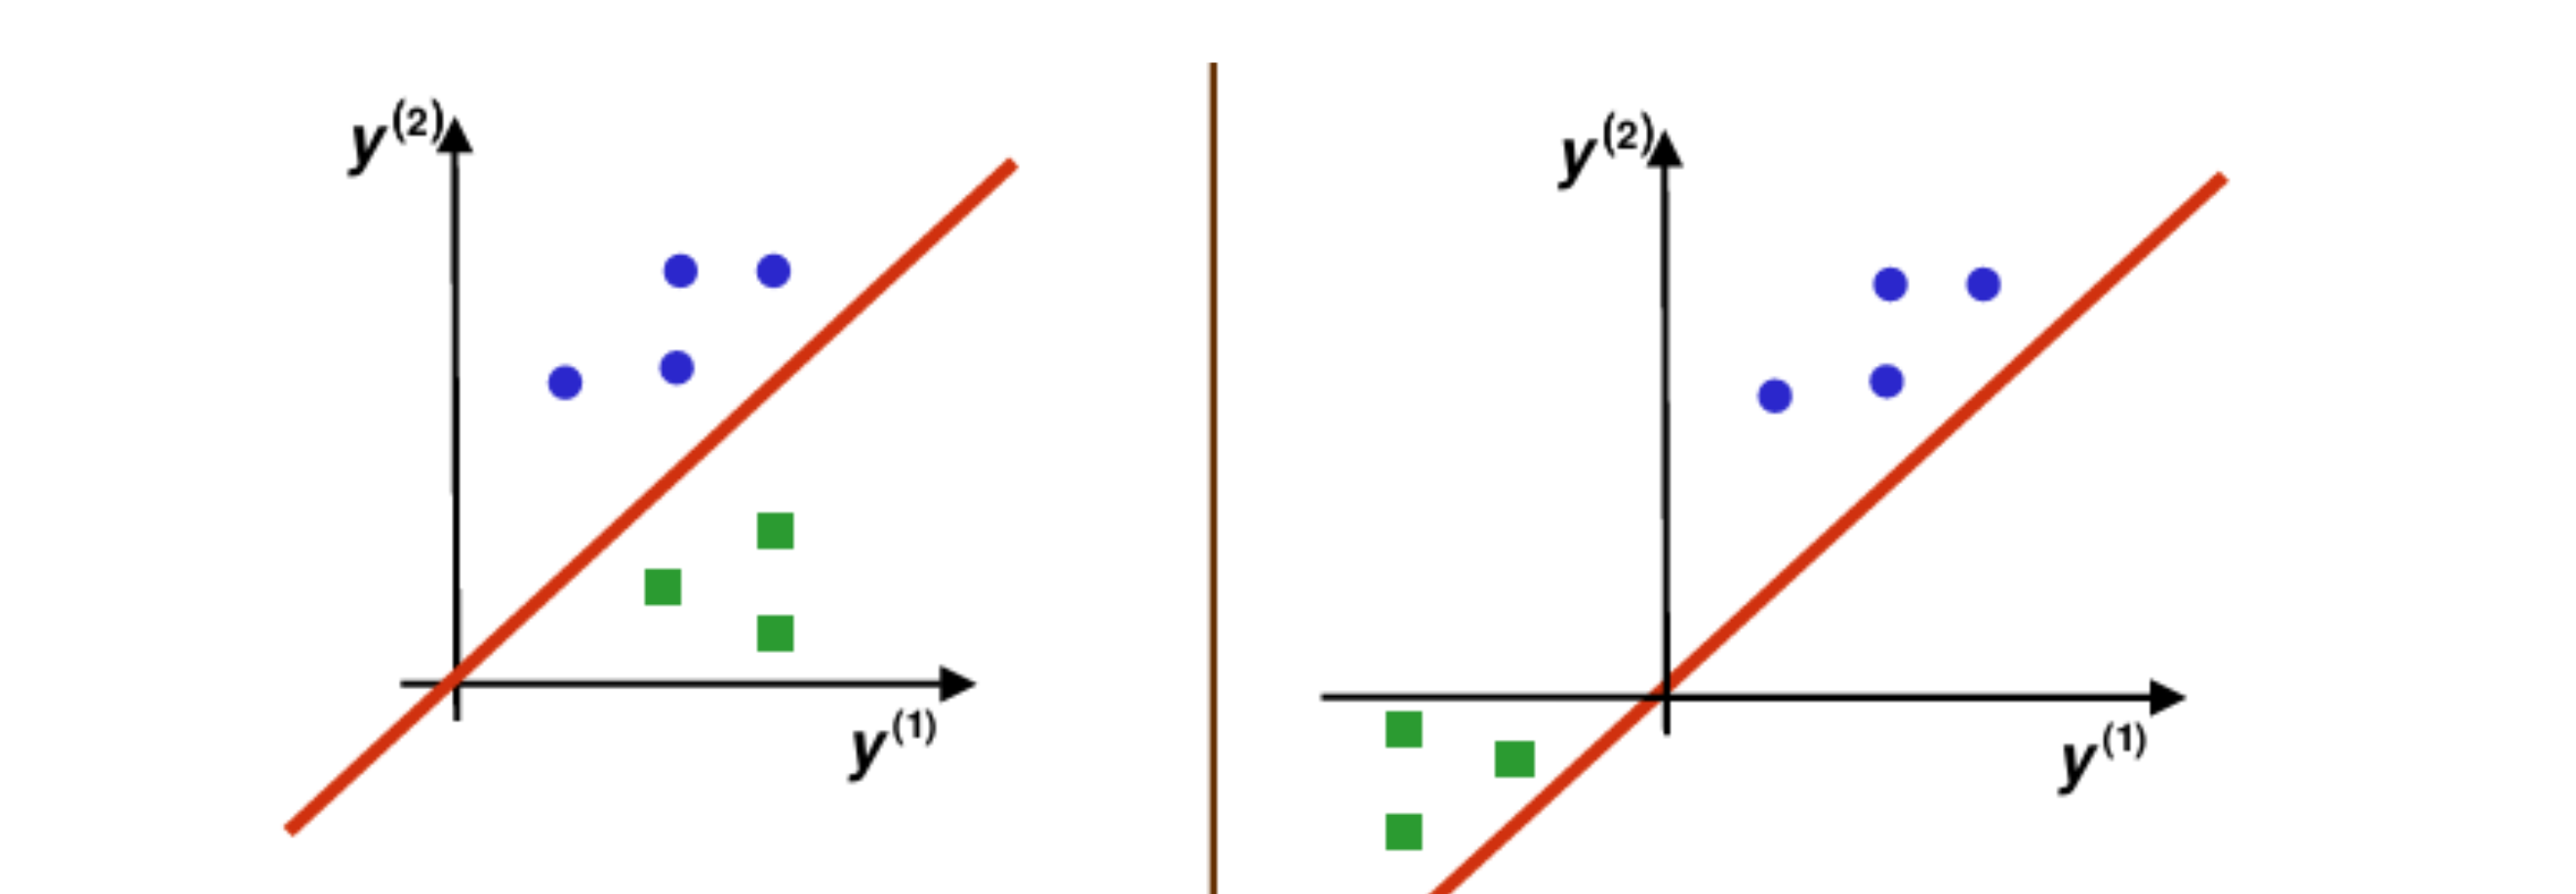
\includegraphics[width=0.6\textwidth]{figures/normalization_diagram.png}
\end{center}

\section{LDF: Solution Region}

Coming back to the "which hyperplane" question...

We can see that many solutions for the weight vector $\mathbf{a}$ exist:
\[
\mathbf{a}^T y_i = \sum_{k=0}^{d} a_k y_i^{(k)} > 0
\]

\begin{tcolorbox}[colback=orange!5!white,colframe=orange!75!black,title=\textbf{Solution Region}]
The \textbf{solution region} corresponding to $\mathbf{a}$ consists of all points classified on one side of the hyperplane, where the hyperplane is perpendicular to the \textbf{normal vector $\mathbf{a}$}.
\end{tcolorbox}

\begin{center}
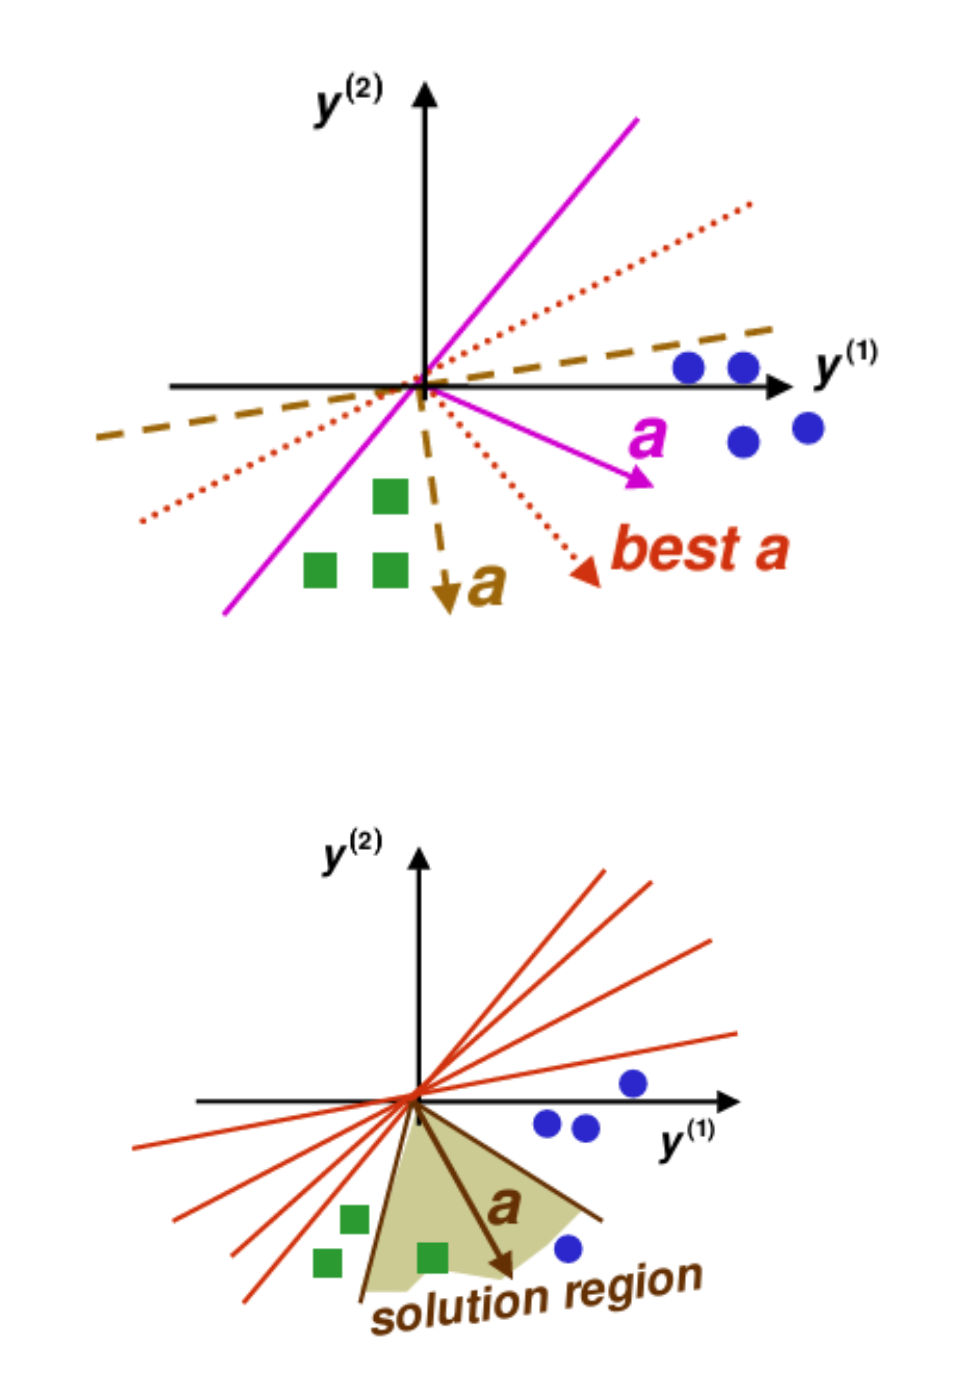
\includegraphics[width=0.6\textwidth]{figures/solution_region.png}
\end{center}

\section{Gradient Descent}

\textbf{Gradient Descent} is one of the simplest approaches to calculating a discriminant function.

It is an iterative method for progressively adjusting the \textbf{weights}.

\begin{tcolorbox}[colback=red!5!white,colframe=red!75!black,title=\textbf{Key Principle}]
The gradient vector in space $\mathbf{W}$ points to the direction of \textbf{maximum deviation} of a function to be maximized/minimized.
\end{tcolorbox}

\begin{center}
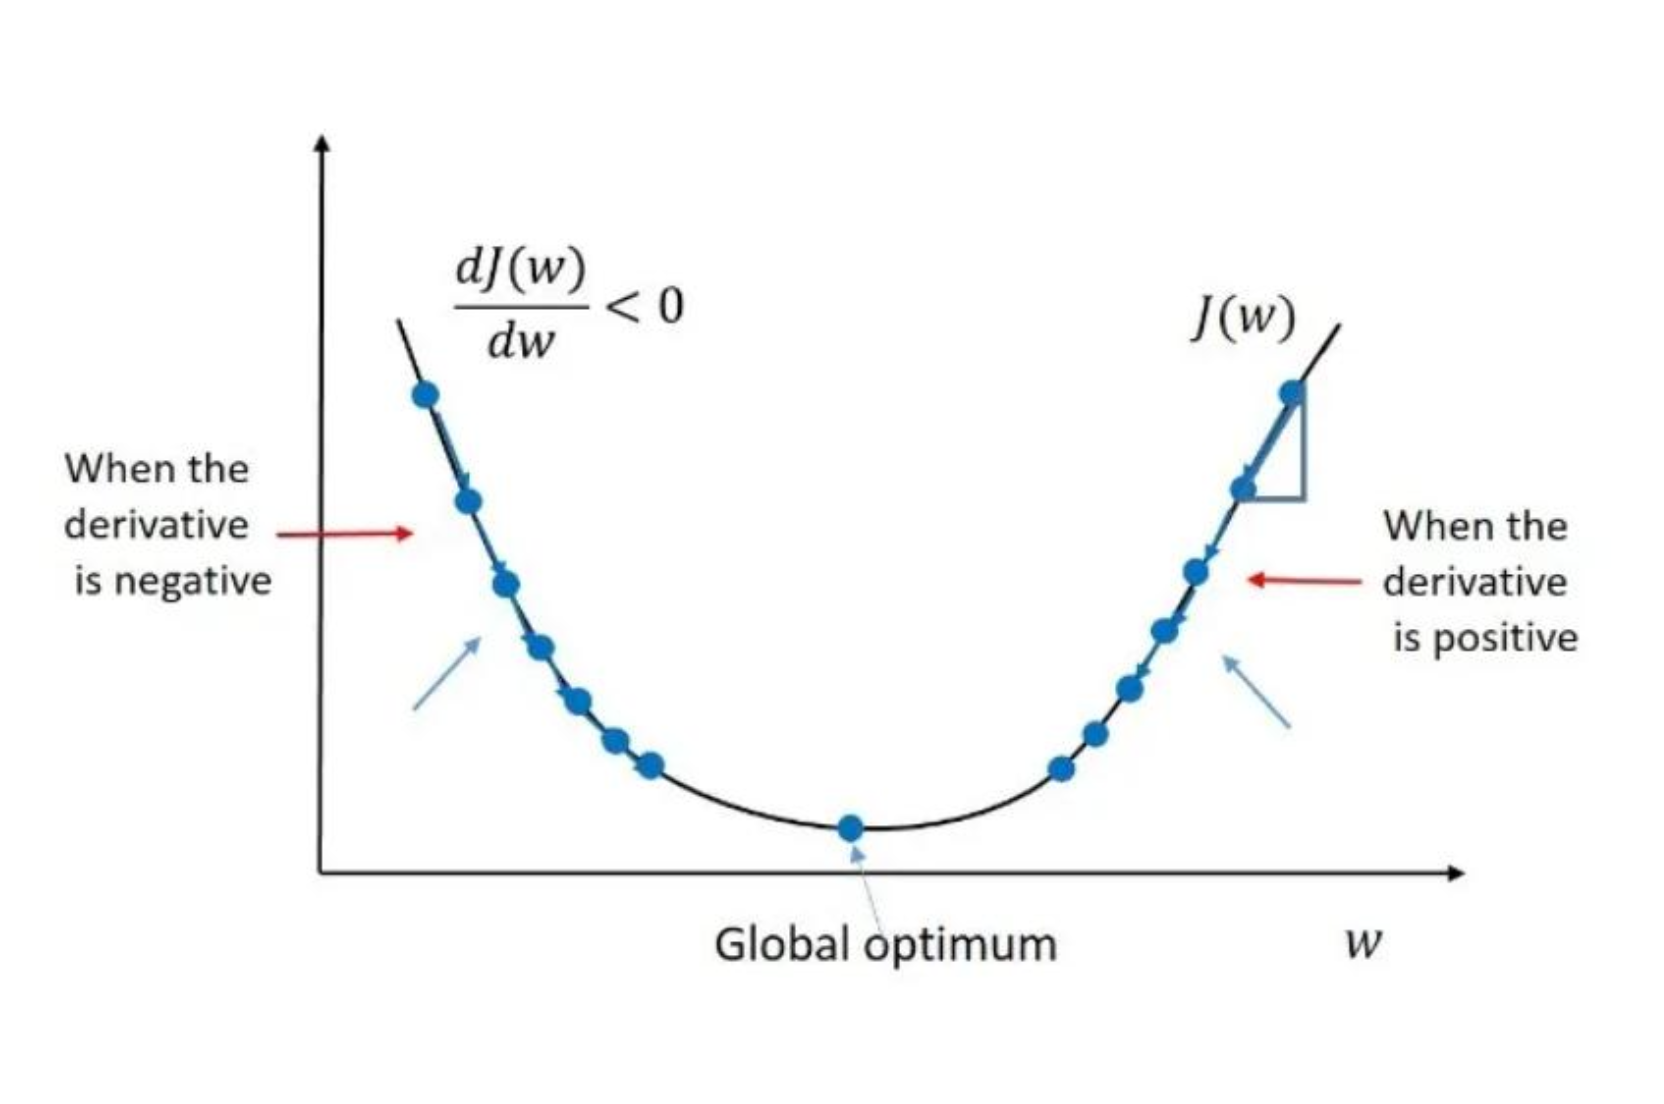
\includegraphics[width=0.5\textwidth]{figures/gradient_descent_intro.png}
\end{center}

\subsection{Gradient Descent Update Rule}

The procedure consists of updating the value of the weight vector at the $k+1$ step with a contribution proportional to the gradient module calculated at the previous step:

\begin{tcolorbox}[colback=green!5!white,colframe=green!75!black,title=\textbf{Gradient Descent Formula}]
\[
\mathbf{w}(k+1) = \mathbf{w}(k) - \rho_k \nabla J(\mathbf{w})\big|_{\mathbf{w}=\mathbf{w}(k)}
\]

where $J(\mathbf{w})$ is an \textbf{evaluation function} (\textit{loss function}) that must be \textbf{minimized}.

\begin{itemize}
    \item $J(\mathbf{w})$ is chosen in such a way as to reach \textbf{the minimum} when $\mathbf{w}$ approaches the \textbf{optimal solution}
    
    \item That is, $J(\mathbf{w})$ should be convex, and $\mathbf{w}$ is the solution vector
\end{itemize}
\end{tcolorbox}

where:
\begin{itemize}
    \item $\rho_k$ is the \textbf{learning rate} (step size) at iteration $k$
    \item $\nabla J(\mathbf{w})$ is the \textbf{gradient} of the loss function
\end{itemize}

\subsection{Local vs Global Minimum}

\begin{itemize}
    \item The minimum of $J(\mathbf{w})$ is obtained by moving $\mathbf{w}$ in the direction opposite to the gradient (in the direction of steepest descent)
    
    \item Gradient descent is guaranteed to find only a \textbf{local minimum}
    
    \item Very popular, as it is simple and applicable to any function
\end{itemize}

\begin{center}
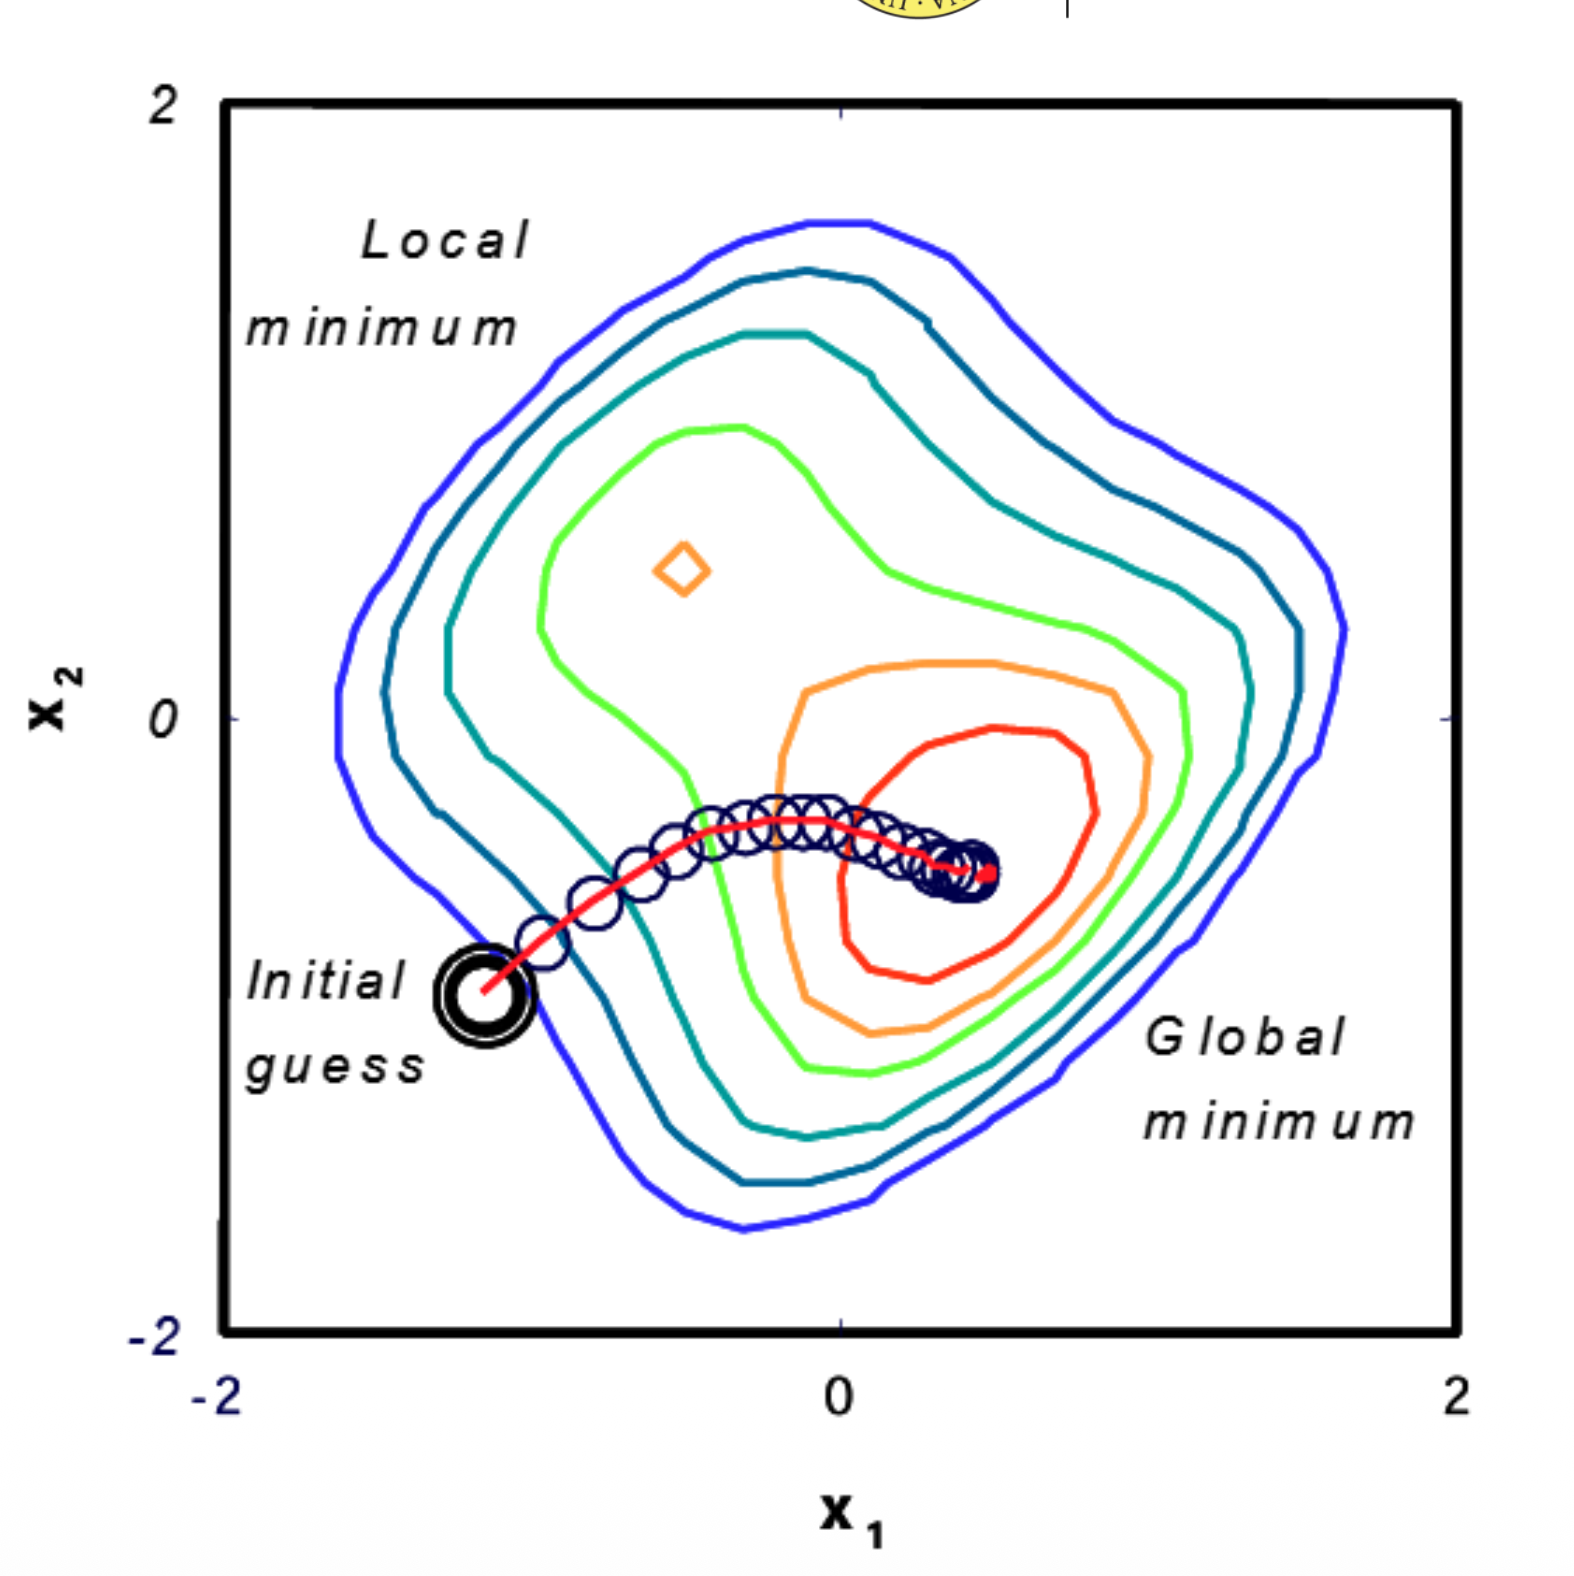
\includegraphics[width=0.6\textwidth]{figures/gradient_descent_local_minimum.png}
\end{center}

\subsection{Gradient Operator}

$\nabla$ is the gradient operator symbol, given by:
\[
\nabla J = \begin{bmatrix}
\frac{\partial J}{\partial w_1} \\
\vdots \\
\vdots \\
\vdots \\
\frac{\partial J}{\partial w_n}
\end{bmatrix}
\]

The update rule remains:
\[
\mathbf{w}(k+1) = \mathbf{w}(k) - \rho_k \nabla J(\mathbf{w})\big|_{\mathbf{w}=\mathbf{w}(k)}
\]

$\rho_k$ (\textbf{learning rate}) is an appropriate scalar value that varies with the iteration $k$, fixing the "magnitude" of the correction.

\subsection{Gradient Descent Summary}

\begin{tcolorbox}[colback=cyan!5!white,colframe=cyan!75!black,title=\textbf{Gradient Descent Algorithm}]
To summarize, at the k-th iteration:
\begin{enumerate}
    \item Start with a chosen weight vector $\mathbf{w}(1)$ and calculate its gradient $J(\mathbf{w}(1))$
    
    \item Then, move from $\mathbf{w}(1)$ in the direction of the steepest descent (opposite to the gradient) by a fixed step size $\rho_k$ to obtain the new vector $\mathbf{w}(2)$
\end{enumerate}

\textbf{Main issue}: How to determine the optimal choice of $\rho_k$
\end{tcolorbox}

\subsection{Learning Rate Selection}

The choice of learning rate $\rho_k$ is critical:

\begin{itemize}
    \item If $\rho_k$ is too \textbf{large}, gradient descent may overshoot the minimum and possibly never find the minimum
    
    \item If $\rho_k$ is too \textbf{small}, it needs too many iterations
\end{itemize}

\begin{center}
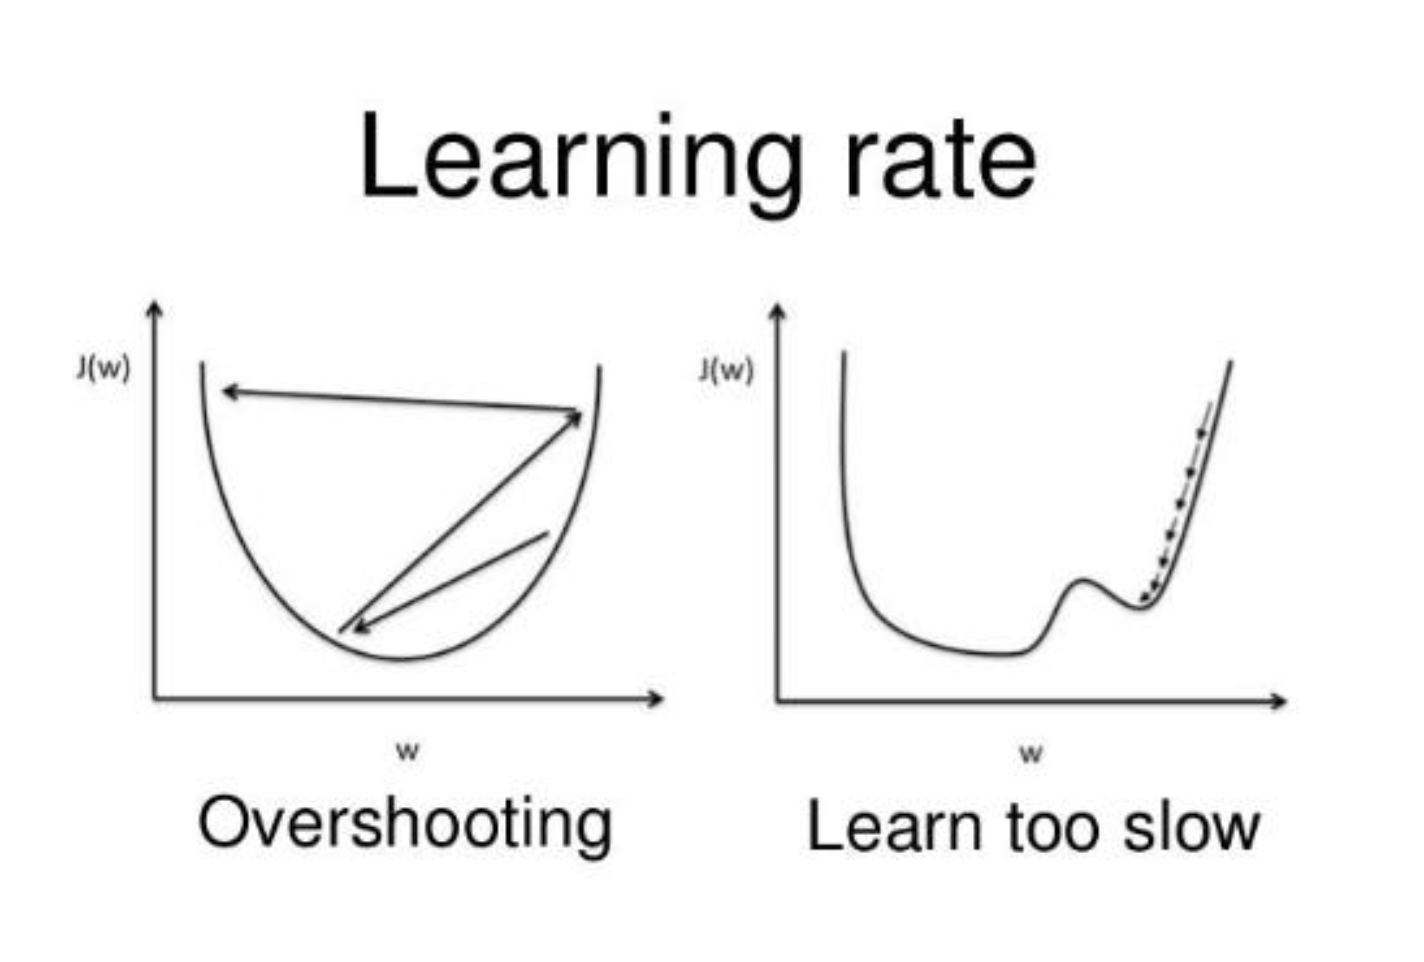
\includegraphics[width=0.5\textwidth]{figures/learning_rate_comparison.png}
\end{center}

\section{Perceptron}

Let's learn a \textbf{binary classifier} with linear discriminant function.

\begin{tcolorbox}[colback=yellow!10!white,colframe=yellow!75!black,title=\textbf{Important Note}]
From this point to the rest, $\mathbf{w}$ and $\mathbf{x}$ are used for an \textbf{augmented feature vector} for simplicity, instead of using $\mathbf{a}$ and $\mathbf{y}$.
\end{tcolorbox}

To do so, we need to choose a $J(\mathbf{w})$ such that the gradient descent can solve it, in this way we can find the minimum of $J(\mathbf{w})$.

\subsection{Perceptron Criterion Function}

\begin{tcolorbox}[colback=red!5!white,colframe=red!75!black,title=\textbf{Perceptron Criterion Function}]
A good choice is the \textbf{Perceptron criterion function}:
\[
J(\mathbf{w}) = -\sum_{i \in X} \mathbf{w}^T \mathbf{x}_i
\]
where $X$ is a set of \textbf{samples misclassified} by $\mathbf{w}$.

\textbf{Key property}: $J(\mathbf{w})$ is non-negative since $\mathbf{w}^T \mathbf{x}_i < 0$ for all misclassified samples.
\end{tcolorbox}

\textbf{Important}: Do not forget to "normalize" the training set by replacing all examples from class $\omega_2$ with their negatives.

\subsection{Convergence Limitation}

We want to use gradient descent to solve the $J(\mathbf{w})$ so that it can converge; however, for such data (not linearly separable), we cannot converge.

\begin{center}
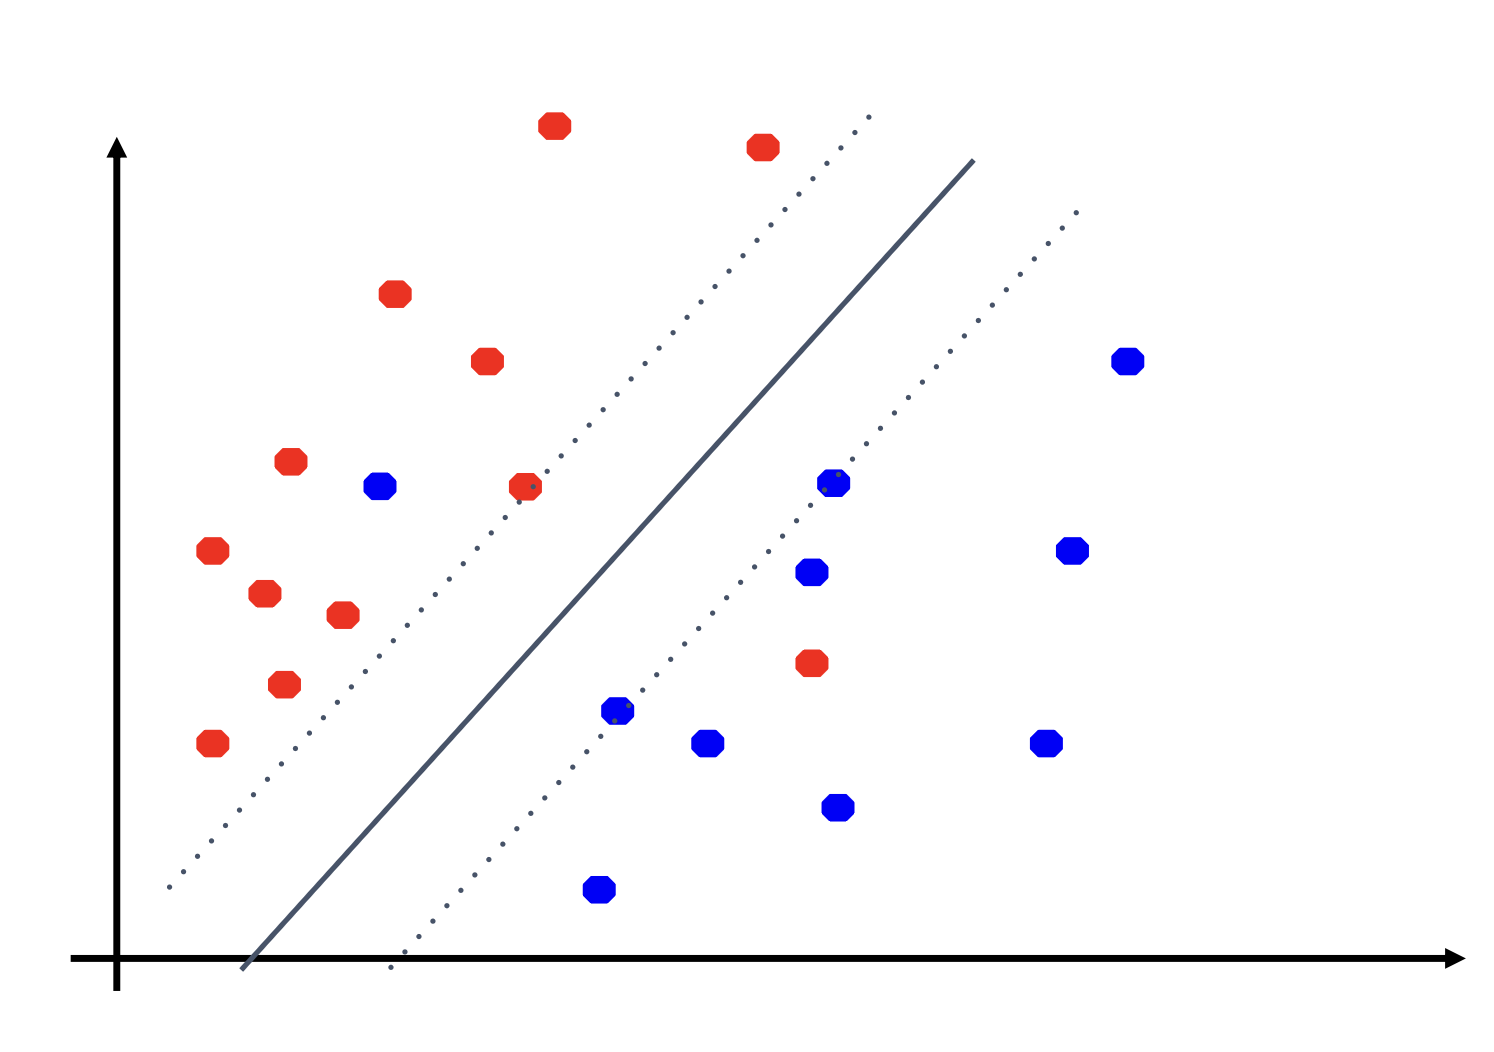
\includegraphics[width=0.5\textwidth]{figures/perceptron_nonseparable.png}
\end{center}

\subsection{Perceptron Gradient Descent}

To find the minimum of $J(\mathbf{w})$, we use gradient descent, which is defined by:

\begin{itemize}
    \item $i$-th component of the gradient of $J(\mathbf{w})$ is equal to $\partial J/\partial w_i$, thus:
\end{itemize}

\[
J(\mathbf{w}) = -\sum_{i \in X} \mathbf{w}^T \mathbf{x}_i \quad \Rightarrow \quad \nabla J = -\sum_{i \in X} \mathbf{x}_i
\]

Note that this does not depend on $\mathbf{w}$.

\begin{tcolorbox}[colback=orange!10!white,colframe=orange!75!black,title=\textbf{Perceptron Rule}]
The update rule becomes:
\[
\mathbf{w}_{k+1} = \mathbf{w}_k + \rho_k \cdot \sum_{i \in X} \mathbf{x}_i, \quad \text{when } \rho_k = \frac{1}{k}
\]

This is known as the \textbf{Perceptron rule}.
\end{tcolorbox}

\textbf{Historical note}: Perceptron is the first \textbf{Neural Network}, which was then evolved to more complex versions such as \textbf{Multilayer Perceptron}.

\subsection{Perceptron Example (Non-Separable Scenario)}

Suppose we have 2 features and 5 samples for 2 classes:
\begin{itemize}
    \item Class 1: $[2,1]$, $[4,3]$, $[3,5]$
    \item Class 2: $[1,3]$, $[5,6]$
\end{itemize}

These samples are not separable with a line, still we will try to get approximate separation by a line.

Obtain the augmented features and normalize the data, by doing so we obtain:
\[
\begin{bmatrix} 1 \\ 2 \\ 1 \end{bmatrix}, 
\begin{bmatrix} 1 \\ 4 \\ 3 \end{bmatrix}, 
\begin{bmatrix} 1 \\ 3 \\ 5 \end{bmatrix}, 
\begin{bmatrix} -1 \\ -1 \\ -3 \end{bmatrix}, 
\begin{bmatrix} -1 \\ -5 \\ -6 \end{bmatrix}
\]

\begin{center}
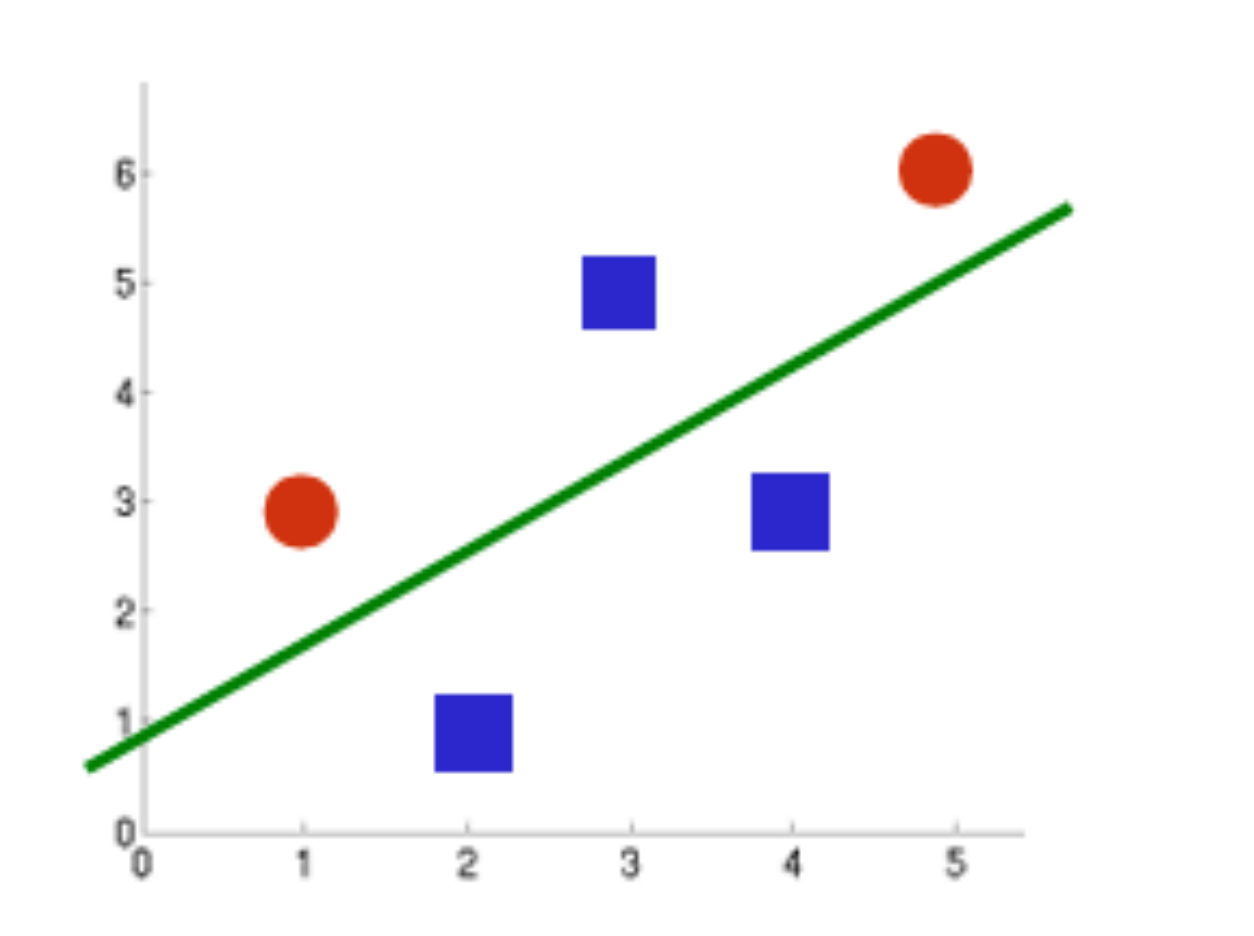
\includegraphics[width=0.5\textwidth]{figures/perceptron_example_setup.png}
\end{center}

\subsection{Applying the Perceptron Method}

Let's apply the perceptron method:
\begin{itemize}
    \item Initial weights $[1 \quad 1 \quad 1]$
    \item This is a line $x_1 + x_2 + 1 = 0$
    \item Fixed learning rate $\rho(k) = 1$
\end{itemize}

\textbf{Iteration 1:}
\begin{align*}
\mathbf{w}_1^{\mathrm{T}} \mathbf{x}_1 &\Rightarrow [1 \; 1 \; 1][1 \; 2 \; 1]^{\mathrm{T}} > 0 \\
\mathbf{w}_1^{\mathrm{T}} \mathbf{x}_2 &\Rightarrow [1 \; 1 \; 1][1 \; 4 \; 3]^{\mathrm{T}} > 0 \\
\mathbf{w}_1^{\mathrm{T}} \mathbf{x}_3 &\Rightarrow [1 \; 1 \; 1][1 \; 3 \; 5]^{\mathrm{T}} > 0
\end{align*}

\begin{align*}
\mathbf{w}_1^{\mathrm{T}} \mathbf{x}_4 &\Rightarrow [1 \; 1 \; 1][-1 \; -1 \; -3]^{\mathrm{T}} = -5 < 0 \\
&\text{Update w!!!} \; \mathbf{w}_2 = [1 \; 1 \; 1] + [-1 \; -1 \; -3] = [0 \; 0 \; -2]
\end{align*}

\textbf{Continue iteration:}
\[
\mathbf{w}_2^{\mathrm{T}} \mathbf{x}_5 \Rightarrow [0 \; 0 \; -2][-1 \; -5 \; -6]^{\mathrm{T}} > 0
\]

\textbf{Iteration 2:}
\[
\mathbf{w}_2^{\mathrm{T}} \mathbf{x}_1 \Rightarrow [0 \; 0 \; -2][1 \; 2 \; 1]^{\mathrm{T}} < 0
\]
Update w again!!!
\[
\mathbf{w}_3 = [0 \; 0 \; -2] + [1 \; 2 \; 1] = [1 \; 2 \; -1]
\]

$\ldots$

$\ldots$

\begin{tcolorbox}[colback=red!10!white,colframe=red!75!black,title=\textbf{Non-Convergence Result}]
We can continue this forever since there is no solution vector $\mathbf{w}$ satisfying the perceptron rule.

The data is \textbf{not linearly separable}, so the perceptron algorithm will not converge to a solution.
\end{tcolorbox}

\subsection{Need for Relaxation}

We want to learn something like this, but our Perceptron constraint does not allow!

\textbf{Solution}: Let's apply some \textbf{relaxation}.

\subsection{Perceptron Summary}

\begin{tcolorbox}[colback=blue!5!white,colframe=blue!75!black,title=\textbf{Perceptron Convergence Properties}]
\begin{itemize}
    \item If classes are \textbf{linearly separable}, the perceptron rule is \textbf{guaranteed to converge} to a valid solution
    \begin{itemize}
        \item Some versions of the perceptron rule use a \textbf{variable learning rate} $\rho(k)$; for now, we fixed it as $1/k$
    \end{itemize}
    
    \item However, if the two classes are \textbf{not linearly separable}, the perceptron rule will \textbf{not converge}
    \begin{itemize}
        \item Since no weight vector $\mathbf{w}$ can correctly classify every sample in a non-separable dataset, the corrections in the perceptron rule will never cease
        
        \item One ad-hoc solution to this problem is to enforce convergence by using variable learning rates $\rho(k)$ that approach zero as $k \rightarrow \infty$
        
        \item We will see once we introduce NN architectures
    \end{itemize}
\end{itemize}
\end{tcolorbox}

\section{The Relaxation Method}

\subsection{Relaxation Criterion Function (1)}

The $J(\mathbf{w})$ takes the form:
\[
J_q(\mathbf{w}) = \sum_{i \in X} (\mathbf{w}^T \mathbf{x}_i)^2
\]

\begin{itemize}
    \item Also, this function takes into account the \textbf{misclassified samples}, and it is minimized when $\mathbf{w}$ is the solution vector
    
    \item Its main difference is that its \textbf{gradient is now continuous}, whereas the gradient of the perceptron function $J$ is not
    
    \item So, such a function is suitable for finding smooth surfaces, but this may lead to problems
    \begin{itemize}
        \item In fact, in this way, the points very far from the origin $(0,0,\ldots,0)$ (i.e., with large feature magnitudes $==$ outliers) are weighted a lot
    \end{itemize}
\end{itemize}

\subsection{Relaxation Criterion Function (2)}

Another option for $J(\mathbf{w})$ is:
\[
J(\mathbf{w}) = \frac{1}{2} \sum_{i \in X} \left\{ \frac{(\mathbf{w}^T \mathbf{x}_i - b)^2}{\|\mathbf{x}_i\|^2} \right\}
\]

where $b \geq 0$ margin (e.g., $b = 1$) and $\mathbf{w}^T \mathbf{x}_i \leq b$.

\begin{itemize}
    \item Dividing by $\|\mathbf{x}_i\|^2$ ensures that samples \textbf{contribute roughly equally}, regardless of their distance from the origin
\end{itemize}

The gradient descent becomes:
\[
\mathbf{w}_{k+1} = \mathbf{w}_k - \rho_k \sum_{i \in X} \left\{ \frac{(\mathbf{w}^T \mathbf{x}_i - b)\mathbf{x}_i}{\|\mathbf{x}_i\|^2} \right\}
\]

with $\mathbf{x}_i$ that verify $\mathbf{w}^T \mathbf{x}_i \leq b$ and $\mathbf{w}$ is calculated with the usual rule.

$J(\mathbf{w}) > 0$ always, and $J(\mathbf{w}) = 0$ if $\mathbf{w}^T \mathbf{x}_i \geq b \; \forall \mathbf{x}_i$

\section{Minimum Squared Error (MSE) Solution}

The classical MSE criterion provides an alternative to the perceptron rule.

\begin{tcolorbox}[colback=green!5!white,colframe=green!75!black,title=\textbf{Key Difference: Perceptron vs MSE}]
\textbf{Perceptron rule}: Only considers \textbf{misclassified samples}, since these are the only ones that violate the $J(\mathbf{w})$.

\textbf{MSE criterion}: Looks for a solution involving \textbf{all of the samples} (not just the misclassified ones).
\begin{itemize}
    \item The goal is to verify $\mathbf{w}^T x_i = b_i$, where the $b_i$ are some arbitrarily specified \textbf{positive constants}
\end{itemize}
\end{tcolorbox}

\subsection{Problem Transformation}

We have replaced the problem of finding the solution to a set of linear inequalities (\textit{perceptron}), now, we have the problem of finding the solution for a set of linear equations (\textit{MSE}).

\begin{itemize}
    \item \textbf{Perceptron}: $\mathbf{w}^T x_i > 0$ for all samples $x_i$, this solves the system of linear inequalities
    
    \item \textbf{MSE}: $\mathbf{w}^T x_i = b_i$ for all samples $x_i$, this solves the system of linear equations
\end{itemize}

\subsection{Comparison: Perceptron Rule vs MSE/Relaxation Method}

\begin{center}
\begin{tabular}{|l|l|l|}
\hline
\textbf{Aspect} & \textbf{Perceptron Rule} & \textbf{MSE / Relaxation Method} \\
\hline
Loss function & Step / misclassification-based & Continuous quadratic (MSE) \\
\hline
Update & Only for misclassified samples & Gradient descent on all samples \\
\hline
Differentiability & Non-differentiable & Differentiable \\
\hline
Surface & Piecewise constant & Smooth (quadratic) \\
\hline
\end{tabular}
\end{center}

\subsection{MSE Procedure}

\begin{tcolorbox}[colback=purple!5!white,colframe=purple!75!black,title=\textbf{MSE Procedure}]
\begin{enumerate}
    \item Choose positive constants $b_1, b_2, \ldots, b_n$
    
    \item Try to find a weight vector $\mathbf{w}$ such that $\mathbf{w}^T \mathbf{x}_i = b_i$ for all samples $x_i$
    
    \item If we can find a weight vector $\mathbf{w}$ such that $\mathbf{w}^T \mathbf{x}_i = b_i$ for all samples $x_i$, then $\mathbf{w}$ is a solution because $b_i$'s are all positive
    
    \item Consider all the samples
\end{enumerate}
\end{tcolorbox}

\subsection{Normalization and Dataset Setup}

For consistency, we will continue assuming that examples from class $\omega_2$ have been replaced by their \textbf{negative vector}, although this is not a requirement for the MSE solution. Thus, we have:
\[
x_{i,n+1} = 1 \text{ for } \omega_1 \quad \text{and} \quad x_{i,n+1} = -1 \text{ for } \omega_2
\]

Suppose we have the following dataset:
\begin{align*}
\text{1st sample: } & x_{1,1}w_1 + x_{1,2}w_2 + \ldots + x_{1,n}w_n + x_{1,n+1}w_{n+1} = b_1, \quad b_1 \geq 0 \\
\text{2nd sample: } & x_{2,1}w_1 + x_{2,2}w_2 + \ldots + x_{2,n}w_n + x_{2,n+1}w_{n+1} = b_2, \quad b_2 \geq 0 \\
& \ldots \\
\text{N-th sample: } & x_{N,1}w_1 + x_{N,2}w_2 + \ldots + x_{N,n}w_n + x_{N,n+1}w_{n+1} = b_N, \quad b_N \geq 0
\end{align*}

\subsection{Matrix Formulation}

We then obtain N equations (equal to the training samples, $N_1$ for $\omega_1$ and $N_2$ for $\omega_2$), with $N = N_1 + N_2$.

We need to solve N equations.

In matrix notation we have: $\mathbf{X} \cdot \mathbf{w} = \mathbf{b}$ where:
\[
\mathbf{X} = \begin{bmatrix}
x_{1,1} & x_{1,2} & \cdots & x_{1,n} & \pm 1 \\
x_{2,1} & \ddots & & \vdots & \vdots \\
\vdots & & \ddots & \vdots & \vdots \\
x_{N,1} & \cdots & \cdots & x_{N,n} & \pm 1
\end{bmatrix}, \quad
\mathbf{b} = \begin{bmatrix}
b_1 \\ b_2 \\ \vdots \\ b_N
\end{bmatrix}, \quad
\mathbf{w} = \begin{bmatrix}
w_1 \\ \vdots \\ w_n \\ w_{n+1}
\end{bmatrix}
\]

Thus, we need to solve a linear system: $\mathbf{X} \cdot \mathbf{w} = \mathbf{b}$

\subsection{Error Vector and MSE Criterion}

Generally, $N >> n+1$, so there are more equations than unknowns.
\[
\mathbf{X} \cdot \mathbf{w} = \mathbf{b} \Rightarrow \mathbf{w} = \mathbf{X}^{-1} \mathbf{b}
\]

Let's now inject the \textbf{error vector} (needed to obtain the loss function), defined as:
\[
\mathbf{e} = \mathbf{X}\mathbf{w} - \mathbf{b}
\]
(imagine this as $\mathbf{b}$ is the real class label and $\mathbf{X}\mathbf{w}$ is your predictions)

MSE finds $\mathbf{w}$ which minimises the length of the error vector $\mathbf{e}$. Thus, minimise the \textbf{minimum squared error} criterion function $J(\mathbf{w})$:
\[
J_M(\mathbf{w}) = (\mathbf{X}\mathbf{w} - \mathbf{b})^{\mathrm{T}} (\mathbf{X}\mathbf{w} - \mathbf{b}) = \| \mathbf{X}\mathbf{w} - \mathbf{b} \|^2
\]

\subsection{Analytical Solution}

Unlike the perceptron criterion, the MSE function is quadratic and differentiable.

Therefore, we can find its minimum \textbf{analytically} by setting the gradient to zero.

The gradient of the objective function $J_M(\mathbf{w})$:
\begin{itemize}
    \item Find derivative of $J_M(\mathbf{w})$ wrt. to $\mathbf{w}$
\end{itemize}

Given $J_M(\mathbf{w}) = (\mathbf{X}\mathbf{w} - \mathbf{b})^{\mathrm{T}} (\mathbf{X}\mathbf{w} - \mathbf{b}) = \| \mathbf{X}\mathbf{w} - \mathbf{b} \|^2$ in matrix format, we differentiate the expression $(\mathbf{X}\mathbf{w} - \mathbf{b})^{\mathrm{T}} (\mathbf{X}\mathbf{w} - \mathbf{b})$ with respect to $\mathbf{w}$.

Let's denote $Y = \mathbf{X}\mathbf{w} - \mathbf{b}$, \textbf{then} $J_M(\mathbf{w}) = Y^{\mathrm{T}} Y$

\subsection{Gradient Derivation}

Now, differentiating $J_M(\mathbf{w})$ wrt. $\mathbf{w}$, we have:
\[
\frac{dJ_M(\mathbf{w})}{d\mathbf{w}} = \frac{d}{d\mathbf{w}}(Y^{\mathrm{T}}Y)
\]

Remember the chain rule, if not clear to you:
\[
= 2Y^{\mathrm{T}} \frac{dY}{d\mathbf{w}} \quad \Rightarrow \quad \frac{dY}{d\mathbf{w}} = \frac{d}{d\mathbf{w}}(\mathbf{X}\mathbf{w} - \mathbf{b}) = \mathbf{X}
\]

Therefore,
\[
\frac{dJ_M(\mathbf{w})}{d\mathbf{w}} = 2Y^{\mathrm{T}} \mathbf{X} = 2(\mathbf{X}\mathbf{w} - \mathbf{b})^{\mathrm{T}} \mathbf{X}
\]

\subsection{Finding the Optimal Solution}

\begin{tcolorbox}[colback=cyan!10!white,colframe=cyan!75!black,title=\textbf{Pseudoinverse Solution}]
By setting the \textbf{gradient to zero}, this becomes:
\[
2(\mathbf{X}\mathbf{w} - \mathbf{b})^{\mathrm{T}} \mathbf{X} = 0 \Rightarrow \mathbf{X}^{\mathrm{T}} \mathbf{X} \mathbf{w} = \mathbf{X}^{\mathrm{T}} \mathbf{b}
\]

(the proof can be found below)

If we multiply by $[\mathbf{X}^{\mathrm{T}} \mathbf{X}]^{-1}$, we get:
\[
\mathbf{w} = [\mathbf{X}^{\mathrm{T}} \mathbf{X}]^{-1} \mathbf{X}^{\mathrm{T}} \mathbf{b} = \mathbf{X}^{\#} \mathbf{b}
\]

where $\mathbf{X}^{\#} = [\mathbf{X}^{\mathrm{T}} \mathbf{X}]^{-1} \mathbf{X}^{\mathrm{T}}$ is the \textbf{pseudoinverse} of $\mathbf{X}$.

\textbf{Consequently}, $\mathbf{w} = \mathbf{X}^{\#} \mathbf{b}$ is the optimal solution according to the MSE method.
\end{tcolorbox}

\subsection{Proof of the Gradient Result}

Starting from:
\[
2(\mathbf{X}\mathbf{w} - \mathbf{b})^{\mathrm{T}} \mathbf{X} = 0
\]

\textbf{Step 1}: Since we have a factor of 2 on the left side, divide both sides by 2:
\[
(\mathbf{X}\mathbf{w} - \mathbf{b})^{\mathrm{T}} \mathbf{X} = 0
\]

\textbf{Step 2}: The expression $(\mathbf{X}\mathbf{w} - \mathbf{b})^{\mathrm{T}} \mathbf{X} = 0$ can be rewritten by expanding the transpose:
\[
(\mathbf{X}\mathbf{w})^{\mathrm{T}} \mathbf{X} - \mathbf{b}^{\mathrm{T}} \mathbf{X} = 0
\]

\textbf{Step 3}: We know that $(\mathbf{X}\mathbf{w})^{\mathrm{T}} \mathbf{X} = \mathbf{w}^{\mathrm{T}} \mathbf{X}^{\mathrm{T}} \mathbf{X}$ (since $(\mathbf{A}\mathbf{B})^{\mathrm{T}} = \mathbf{B}^{\mathrm{T}} \mathbf{A}^{\mathrm{T}}$):
\[
\mathbf{w}^{\mathrm{T}} \mathbf{X}^{\mathrm{T}} \mathbf{X} - \mathbf{b}^{\mathrm{T}} \mathbf{X} = 0
\]

\textbf{Step 4}: This equality holds if:
\[
\mathbf{X}^{\mathrm{T}} \mathbf{X} \mathbf{w} = \mathbf{X}^{\mathrm{T}} \mathbf{b}
\]

This is the desired result, so we have shown that:
\[
2(\mathbf{X}\mathbf{w} - \mathbf{b})^{\mathrm{T}} \mathbf{X} = 0 \Rightarrow \mathbf{X}^{\mathrm{T}} \mathbf{X} \mathbf{w} = \mathbf{X}^{\mathrm{T}} \mathbf{b}
\]

\section{MSE Properties}

\begin{tcolorbox}[colback=orange!5!white,colframe=orange!75!black,title=\textbf{Dependence on Margin Vector}]
$\mathbf{w} = \mathbf{X}^{\#} \mathbf{b}$ shows that the MSE solution depends on the \textbf{margin vector $\mathbf{b}$}.

\begin{itemize}
    \item Different choices of $\mathbf{b}$ lead to different properties of the solution
\end{itemize}
\end{tcolorbox}

\begin{itemize}
    \item If $\mathbf{b}$ is arbitrarily fixed, there is no evidence that the MSE solution gives a separator vector in the case of linear separability
    
    \item So, how to choose $\mathbf{b}$ in the MSE procedure?
    \begin{itemize}
        \item Good choice is $b_1 = b_2 = \ldots = B_n = 1$. In this case, the MSE solution is identical to Fischer's linear discriminant solution (\textit{next lesson})
    \end{itemize}
\end{itemize}

\subsection{Sensitivity to Outliers}

\begin{tcolorbox}[colback=red!10!white,colframe=red!75!black,title=\textbf{Warning: Outlier Sensitivity}]
MSE pays too much attention to \textbf{outlier examples}!

\begin{itemize}
    \item Because MSE squares the error, \textbf{large errors (outliers)} have a disproportionately large influence on the solution
    
    \item For classification, where we only care about \textit{which side} of the boundary a sample is on, this sensitivity is undesirable
\end{itemize}
\end{tcolorbox}

\subsection{Computational Challenges}

$\mathbf{X}^{\#}$ is difficult to obtain:
\begin{itemize}
    \item As this requires inverting a large matrix, which is:
    \begin{itemize}
        \item \textbf{expensive} for high-dimensional data
        \item \textbf{impossible} if $\mathbf{X}^{\mathrm{T}}\mathbf{X}$ is \textbf{singular} (non-invertible)
    \end{itemize}
    
    \item The analytical solution is \textit{computationally heavy} and sometimes \textit{ill-defined}
\end{itemize}

\subsection{Lack of Flexibility}

It is not an iterative process, indeed, $\mathbf{w}$ is obtained directly through mathematical computations in \textbf{one step}.

\begin{itemize}
    \item Even if this sounds good,
    \item it means we \textbf{lose flexibility}
    \begin{itemize}
        \item E.g., no gradual correction
        \item online learning
    \end{itemize}
\end{itemize}

\section{Example: Perceptron vs MSE}

Compute the \textbf{perceptron} and \textbf{MSE} solution for the dataset:

\textbf{Class 1 (X1)}: $[(1,6), (7,2), (8,9), (9,9)]$

\textbf{Class 2 (X2)}: $[(2,1), (2,2), (2,4), (7,1)]$

\subsection{Perceptron Learning}

Assume $\rho_k = 0.1$ and an online update rule.

Assume $\mathbf{w}_1 = [0.1, 0.1, 0.1]$

\textbf{Step 1}: Normalize the dataset (augment features and replace class 2 with negatives):
\[
\begin{bmatrix}
1 & 1 & 6 \\
1 & 7 & 2 \\
1 & 8 & 9 \\
1 & 9 & 9 \\
-1 & -2 & -1 \\
-1 & -2 & -2 \\
-1 & -2 & -4 \\
-1 & -7 & -1
\end{bmatrix}
\]

\subsection{Perceptron Iteration}

\textbf{Step 2}: Iterate through all the examples ($\mathbf{w}^{\mathrm{T}}\mathbf{x}_i$) and update $\mathbf{w}(k)$:

\textit{Data point 1}: $[0.1 \; 0.1 \; 0.1]^{\mathrm{T}} [1 \; 1 \; 6]$ this is $>0$ so correctly classified, therefore there is no update

\textit{Data point 2}: $[0.1 \; 0.1 \; 0.1]^{\mathrm{T}} [1 \; 7 \; 2]$ this is $>0$ so correctly classified, therefore there is no update

$\ldots$

\textit{Data point 5}: $[0.1 \; 0.1 \; 0.1]^{\mathrm{T}} [-1 \; -2 \; -1]$ this is $<0$ so we have to apply an update:
\[
\mathbf{w}(2) = \mathbf{w}(1) + \rho_1 [-1 \; -2 \; -1] = [0 \; -0.1 \; 0]
\]

$\ldots$

\textit{Data point 1}: $[0 \; -0.1 \; 0]^{\mathrm{T}} [1 \; 1 \; 6]$ this is $<0$ so update:
\[
\mathbf{w}(3) = \mathbf{w}(2) + \rho_1 [1 \; 1 \; 6] = [0 \; -0.1 \; 0] + 0.1[1 \; 1 \; 6] = [0.1 \; 0 \; 0.6]
\]

\textit{Data point 2}: $[0.1 \; 0 \; 0.6]^{\mathrm{T}} [1 \; 7 \; 2] > 0 \Rightarrow$ no update

$\ldots$

\textbf{The perceptron with this data and setup converges after 175 iterations, when $\mathbf{w} = [-3.5 \; 0.3 \; 0.7]$}

\subsection{MSE Solution}

\textbf{MSE}: This solution will be found in one shot $\mathbf{w} = [\mathbf{X}^{\mathrm{T}} \mathbf{X}]^{-1} \mathbf{X}^{\mathrm{T}} \mathbf{b}$

For the choice of $\mathbf{b} = [1 \; 1 \; 1 \; 1 \; 1 \; 1 \; 1 \; 1]$, the solution is:
\[
\mathbf{w} = [-1.1870 \; 0.0746 \; 0.1959]
\]

Dataset:
\begin{itemize}
    \item X1 = $[(1,6), (7,2), (8,9), (9,9)]$
    \item X2 = $[(2,1), (2,2), (2,4), (7,1)]$
\end{itemize}

As seen in the figure, the MSE misclassifies one of the samples.

\section{Perceptron vs. MSE (Summary)}

\begin{tcolorbox}[colback=blue!5!white,colframe=blue!75!black,title=\textbf{Comparison Summary}]
\textbf{Perceptron rule}: The perceptron rule always finds a solution if the classes are linearly separable, but does not converge if the classes are non-separable.

\textbf{MSE criterion}: The MSE solution has guaranteed convergence, but it may not find a separating hyperplane if classes are linearly separable.

\begin{itemize}
    \item Notice that MSE tries to minimize the sum of the squares of the distances of the training data to the separating hyperplane, as opposed to finding this hyperplane
\end{itemize}
\end{tcolorbox}

\subsection{Gradient Descent Alternative for MSE}

The objective function $J_M(\mathbf{w})$ can also be minimized using a gradient descent procedure. In this way, we avoid:
\begin{itemize}
    \item the problems that arise when $\mathbf{X}^{\mathrm{T}} \mathbf{X}$ is singular (happens if samples are correlated)
    \item the need for working with large matrices
\end{itemize}

Since $\nabla J_M(\mathbf{w}) = 2 \mathbf{X}^{\mathrm{T}} (\mathbf{X}\mathbf{w} - \mathbf{b})$, the gradient descent algorithm is:
\[
\mathbf{w}_{k+1} = \mathbf{w}_k - \rho_k \mathbf{X}^{\mathrm{T}} (\mathbf{X}\mathbf{w}_k - \mathbf{b}) \quad \text{with } \mathbf{w}_1 \text{ arbitrary}
\]

[$X$ and $b$ are in matrix and vector form, written for all data]

\begin{tcolorbox}[colback=green!5!white,colframe=green!75!black,title=\textbf{Convergence Property}]
It can be shown that if $\rho_k = \rho_1/k$ where $\rho_1$ is any positive constant, this rule generates a sequence of weight vectors that converge to a solution to:
\[
\mathbf{X}^{\mathrm{T}} (\mathbf{X} \mathbf{w} - \mathbf{b}) = 0
\]

The gradient descent algorithm leads to the solution \textbf{regardless of whether $\mathbf{X}^{\mathrm{T}} \mathbf{X}$ is singular or not}.
\end{tcolorbox}

\section{The Least MSE (LMSE = Widrow-Hoff Method)}

Considering \textbf{one sample at a time}, we get:

\begin{tcolorbox}[colback=yellow!10!white,colframe=yellow!75!black,title=\textbf{LMS Rule}]
\[
\mathbf{w}_{k+1} = \mathbf{w}_k + \rho_k (b_k - \mathbf{w}_k^{\mathrm{T}} \mathbf{x}_k) \mathbf{x}_k
\]

such that $b_k$ is the value for the k-th sample of the margin $\mathbf{b}$ ($b_k \geq 0$), i.e., it depends on the sample $\mathbf{x}_k$.
\end{tcolorbox}

This method is called \textbf{Widrow-Hoff}, \textbf{least-mean-squares (LMS)} or \textbf{delta rule}:
\begin{itemize}
    \item reduces \textbf{storage requirements} by considering single samples \textbf{sequentially}
\end{itemize}

\subsection{Correction Mechanism}

Widrow-Hoff rule "corrects" $\mathbf{w}_k$ whenever $\mathbf{w}_k^{\mathrm{T}} \mathbf{x}_k \neq b_k$.

\textbf{Why?}

The weight change is:
\[
\Delta \mathbf{w}_k = \mathbf{w}_{k+1} - \mathbf{w}_k = \rho_k (b_k - \mathbf{w}_k^{\mathrm{T}} \mathbf{x}_k) \mathbf{x}_k
\]

\textbf{Case 1: Prediction is correct}
\[
\mathbf{w}_k^{\mathrm{T}} \mathbf{x}_k = b_k
\]

then
\[
\Delta \mathbf{w}_k = \rho_k (b_k - \mathbf{w}_k^{\mathrm{T}} \mathbf{x}_k) \mathbf{x}_k = \rho_k (0) \mathbf{x}_k = 0
\]

so $\mathbf{w}_{k+1} = \mathbf{w}_k \rightarrow$ \textbf{no correction happens}.

\subsection{Case 2: Prediction is Wrong}

\[
\mathbf{w}_k^{\mathrm{T}} \mathbf{x}_k \neq b_k
\]

then
\[
\Delta \mathbf{w}_k = \rho_k (b_k - \mathbf{w}_k^{\mathrm{T}} \mathbf{x}_k) \mathbf{x}_k \neq 0
\]

so $\mathbf{w}_{k+1} \neq \mathbf{w}_k \rightarrow$ \textbf{the weight vector is corrected}.

\begin{itemize}
    \item The advantage of "correcting only when $\mathbf{w}_k^{\mathrm{T}} \mathbf{x}_k \neq b_k$" is that learning is \textbf{efficient, stable, proportional, and error-driven}
    
    \item We adjust weights \textbf{exactly when and as much as needed}
\end{itemize}

\subsection{Widrow-Hoff Method: Summary}

\begin{tcolorbox}[colback=cyan!5!white,colframe=cyan!75!black,title=\textbf{Widrow-Hoff Advantages}]
Iterative, gradient-descent-based update:
\[
\mathbf{w}_{k+1} = \mathbf{w}_k + \rho_k (b_k - \mathbf{w}_k^{\mathrm{T}} \mathbf{x}_k) \mathbf{x}_k
\]

\begin{itemize}
    \item Can update \textbf{sample-by-sample}
    \begin{itemize}
        \item Low computational cost per iteration, scalable to large datasets
    \end{itemize}
    
    \item Learning rate controls convergence speed
    
    \item Adapts to new data (suitable for online learning)
\end{itemize}
\end{tcolorbox}

\subsection{Widrow-Hoff Method: Disadvantages}

\begin{itemize}
    \item Can converge slowly
    \begin{itemize}
        \item Sensitive to correlated features and outliers
    \end{itemize}
    
    \item Needs careful learning rate
    
    \item \textbf{Requires multiple iterations; not one-step like analytical MSE}
    
    \item May struggle with non-linear or non-separable data
\end{itemize}

\begin{center}
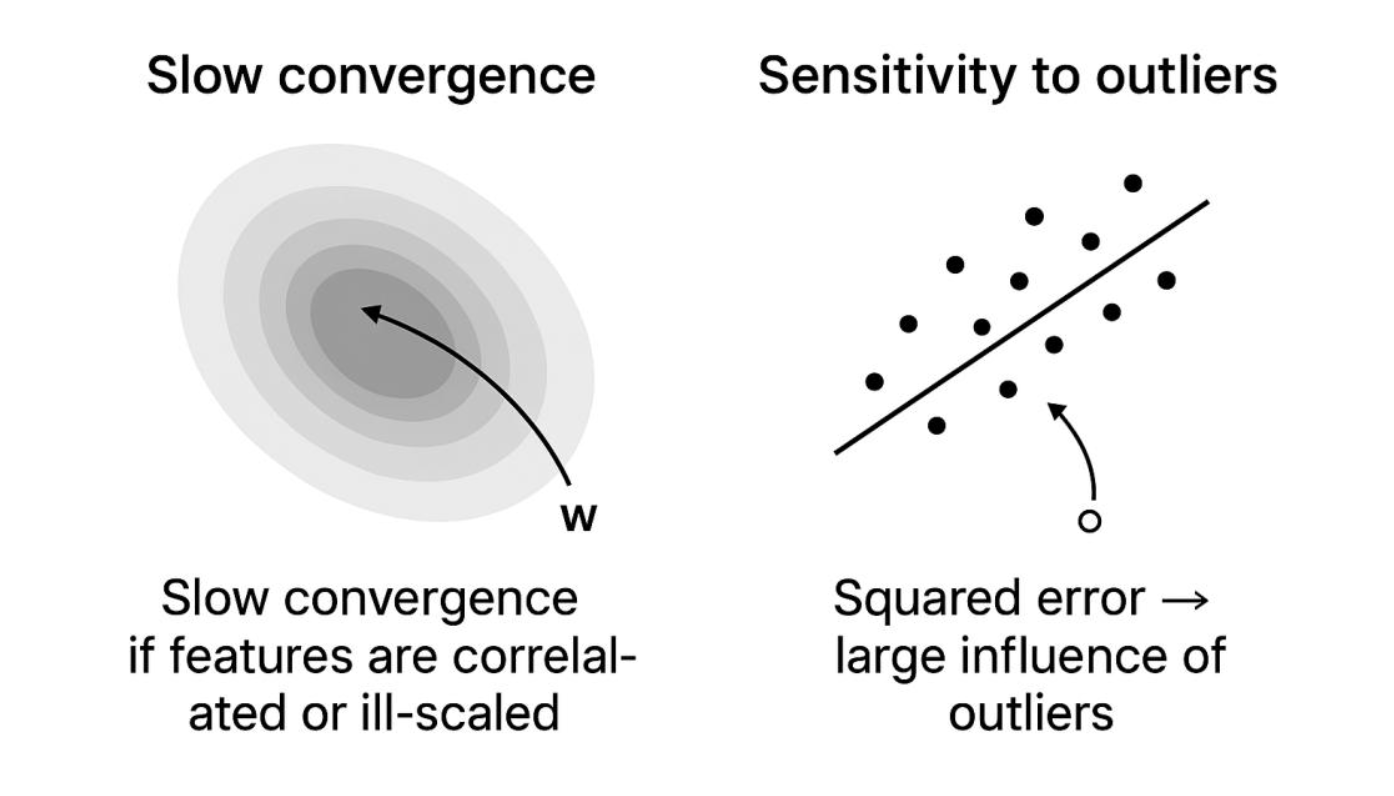
\includegraphics[width=0.6\textwidth]{figures/widrow_hoff_disadvantages.png}
\end{center}

\section{The Ho-Kashyap Method}

\begin{tcolorbox}[colback=red!10!white,colframe=red!75!black,title=\textbf{MSE Limitation}]
The main limitation of the MSE criterion is the \textbf{lack of guarantees} that a separating hyperplane will be found in the linearly separable case.
\end{tcolorbox}

All we can say about the MSE rule is that it minimises $\|\mathbf{X}\mathbf{w} - \mathbf{b}\|^2$ when $\mathbf{b}$ is chosen arbitrarily.

This means that whether MSE finds a separating hyperplane or not depends on how properly the margin $\mathbf{b}$ is selected (notice that in some sources $\mathbf{b}$ is referred to as \textit{target outputs}).

\subsection{Ho-Kashyap Approach}

If the training samples are linearly separable, then there must be vectors $\mathbf{w}^*$ and $\mathbf{b}^*$ such that $\mathbf{X}\mathbf{w}^* = \mathbf{b}^* > 0$ where $\mathbf{b}^* > 0$, meaning that every component of $\mathbf{b}^*$ is \textbf{positive}.

\begin{itemize}
    \item If $\mathbf{b}^*$ were \textbf{known}, one could simply use MSE solution to compute separating hyperplane
    
    \item \textbf{Idea}: find both $\mathbf{w}^*$ and $\mathbf{b}^*$
    
    \item Minimize the following criterion function, restricting to positive $\mathbf{b}$:
    \[
    J_{HK}(\mathbf{w}, \mathbf{b}) = \|\mathbf{X}\mathbf{w} - \mathbf{b}\|^2
    \]
    
    \item $J_{HK}(\mathbf{w}^*, \mathbf{b}^*) = 0$
\end{itemize}

\subsection{Gradient Descent Optimization}

\[
J_{HK}(\mathbf{w}, \mathbf{b}) = \|\mathbf{X}\mathbf{w} - \mathbf{b}\|^2
\]

As usual, take partial derivatives with respect to $\mathbf{w}$ and $\mathbf{b}$:
\begin{align*}
\nabla_{\mathbf{w}} J_{HK} &= -2 \mathbf{W}^{\mathrm{T}} (\mathbf{X}\mathbf{w} - \mathbf{b}) = 0 \\
\nabla_{\mathbf{b}} J_{HK} &= -2 (\mathbf{X}\mathbf{w} - \mathbf{b}) = 0
\end{align*}

Use gradient descent to find a minimum $J_{HK}(\mathbf{w}, \mathbf{b})$.

Alternate the two steps below until convergence:
\begin{itemize}
    \item Fix $\mathbf{b}$ and minimize $J_{HK}(\mathbf{w}, \mathbf{b})$ with respect to $\mathbf{w}$
    \item Fix $\mathbf{w}$ and minimize $J_{HK}(\mathbf{w}, \mathbf{b})$ with respect to $\mathbf{b}$
\end{itemize}

\subsection{Ho-Kashyap Rule}

\begin{tcolorbox}[colback=yellow!10!white,colframe=yellow!75!black,title=\textbf{Ho-Kashyap Rule}]
The resulting iterative \textbf{Ho-Kashyap rule} is:
\[
\mathbf{b}_{k+1} = \mathbf{b}_k - \frac{1}{2}\rho_k [\nabla_{\mathbf{b}} J_{HK}(\mathbf{w}_k, \mathbf{b}_k) - |\nabla_{\mathbf{b}} J_{HK}(\mathbf{w}_k, \mathbf{b}_k)|]
\]

where $\nabla_{\mathbf{b}} J_{HK} = -2 (\mathbf{X}\mathbf{w} - \mathbf{b}) = 0$

Let $\mathbf{e}_k = \mathbf{X}\mathbf{w}_k - \mathbf{b}_k = -\frac{1}{2}[\nabla_{\mathbf{b}} J_{HK}(\mathbf{w}_k, \mathbf{b}_k)]$

Then:
\begin{align*}
\mathbf{b}_{k+1} &= \mathbf{b}_k - \frac{1}{2}\rho_k [-2\mathbf{e}_k - |2\mathbf{e}_k|] \\
&= \mathbf{b}_k + \rho_k [\mathbf{e}_k + |\mathbf{e}_k|]
\end{align*}
\end{tcolorbox}

\subsection{Ho-Kashyap Algorithm}

\begin{tcolorbox}[colback=cyan!5!white,colframe=cyan!75!black,title=\textbf{Ho-Kashyap Algorithm}]
\textbf{(0)} Start with arbitrary $\mathbf{b}_1 > 0$ and $\mathbf{w}_1$, let $k=1$

\textbf{Repeat steps (1) to (4):}

\textbf{(1)} $\mathbf{e}_k = \mathbf{X}\mathbf{w}_k - \mathbf{b}_k$

\textbf{(2)} Solve for $\mathbf{b}_{k+1}$ using $\mathbf{w}_k$ and $\mathbf{b}_k$:
\[
\mathbf{b}_{k+1} = \mathbf{b}_k + [\mathbf{e}_k + |\mathbf{e}_k|]
\]

\textbf{(3)} Solve for $\mathbf{w}_{k+1}$ using $\mathbf{b}_{k+1}$:
\[
\mathbf{w}_{k+1} = (\mathbf{w}^{\mathrm{T}}\mathbf{w})^{-1} Y^{\mathrm{T}} \mathbf{b}_{k+1}
\]

\textbf{(4)} $k = k+1$

\textbf{until} $\mathbf{e}_k = 0$ or $k > k_{max}$ or $\mathbf{b}_{k+1} = \mathbf{b}_k$ (for convergence fix learning rate as $0 < \rho_k < 1$)
\end{tcolorbox}

\subsection{Convergence Properties}

\begin{tcolorbox}[colback=green!5!white,colframe=green!75!black,title=\textbf{Ho-Kashyap Convergence}]
\textbf{In the linearly separable case:}
\begin{itemize}
    \item $\mathbf{e}_k = 0$, solution is found, STOP!
    \item One of the components of $\mathbf{e}_k$ is positive, algorithm continues
\end{itemize}

\textbf{In non-separable case:}
\begin{itemize}
    \item $\mathbf{e}_k$ will have only negative components eventually, thus found proof of non-separability
    \item No bound on how many iterations is needed for the proof of non-separability
\end{itemize}
\end{tcolorbox}

\section{Summary: Linear Discriminant Functions}

\begin{tcolorbox}[colback=purple!5!white,colframe=purple!75!black,title=\textbf{Comparison of Methods}]

\subsection*{Perceptron Procedure}
\begin{itemize}
    \item Find a separating hyperplane in the linearly separable case
    \item Do not converge in the non-separable case
    \item Can force convergence by using a decreasing learning rate, but there is no guarantee of a reasonable stopping point
\end{itemize}

\subsection*{MSE Procedure}
\begin{itemize}
    \item Converge in separable and non-separable cases
    \item May not find a separating hyperplane if classes are linearly separable
    \item Use pseudoinverse if $\mathbf{X}^{\mathrm{T}}\mathbf{X}$ is not singular and not too large
    \item Use gradient descent (Widrow-Hoff procedure) otherwise
\end{itemize}

\subsection*{Ho-Kashyap Procedure}
\begin{itemize}
    \item Always converge
    \item Find a separating hyperplane in the linearly separable case
    \item More costly
\end{itemize}
\end{tcolorbox}




\newpage 

\part{Linear Transformations and Dimensionality Reduction}

\section{Problems of High-Dimensional Data}

In practical problems, training data can appear in various forms:
\begin{itemize}
    \item Few samples
    \item Few samples and many features
    \item Fixed features that cannot be selected
    \item Not-independent features
\end{itemize}

There are two important things to consider when designing a classifier:
\begin{enumerate}
    \item \textbf{Computational complexity} of the system
    \item The \textbf{influence of the dimensionality} (the number of features) of the training set on the performance of the classifier
\end{enumerate}

If the features are statistically \textbf{independent}, then it is more likely to achieve optimal performance. In general, if the performance is not at the desired level, one can add features, but this increases the complexity of both the classifier and the feature extractor.

If adding features leads to \textbf{worse} performance, then this could be because:
\begin{itemize}
    \item Choosing an \textbf{incorrect model} (e.g., Gaussian hypothesis or conditional probability hypothesis)
    \item \textbf{Insufficient number of samples}
\end{itemize}

\subsection{Computational Complexity}

Complexity (in terms of running time) increases when the number of features, i.e., dimensionality $d$, increases. Many methods already have at least $O(nd^2)$ complexity, where $n$ is the number of samples (e.g., covariance matrix calculation). As $d$ increases, this cost may become prohibitive.

\subsection{Curse of Dimensionality}

\begin{definition}[Curse of Dimensionality]
If the dimensionality $d$ is large and the number of samples $n$ is too small, the problem of the \textbf{curse of dimensionality} appears: we cannot perform accurate parameter estimation, classification, etc.
\end{definition}

For example, in the case of covariance matrix calculation, for accurate estimation, $n$ should be much bigger than $d^2$. Otherwise, the model would be too complicated for the data and \textbf{overfitting} occurs.

\textbf{Example with $k$-NN ($k=1$):}
\begin{itemize}
    \item Suppose we have 1 feature and 9 samples. The feature may not be discriminative.
    \item If we add a 2nd feature (same 9 samples), the feature space becomes too sparse for 1-NN to work well. To maintain the same density as in 1D, we would need $9^2 = 81$ samples.
    \item With 3 features, we would need $9^3 = 729$ samples!
\end{itemize}

\begin{tcolorbox}[colback=red!5!white,colframe=red!75!black,title=\textbf{Key Rule}]
If $n$ samples is dense enough in 1D, then in $d$ dimensions we need $n^d$ samples to maintain the same density. The quantity $n^d$ grows extremely fast as a function of $d$.
\end{tcolorbox}

\subsection{Overfitting in High Dimensions}

Overfitting occurs when a model learns to \textbf{perform well on the training data} but \textbf{fails to generalize to unseen data}. When $d$ is high, the data become increasingly sparse and spread out in the high-dimensional space. This can lead to overfitting because:
\begin{itemize}
    \item The model may learn patterns that are specific to the training data
    \item The model has more freedom to fit the noise (e.g., irrelevant features) rather than the underlying patterns
\end{itemize}

For a fixed number of samples, as we add features, the training error keeps decreasing but the validation error eventually increases --- this is overfitting.

\begin{tcolorbox}[colback=blue!5!white,colframe=blue!75!black,title=\textbf{Mitigating Overfitting and the Curse of Dimensionality}]
\begin{itemize}
    \item \textbf{Reduce the dimensionality} of features (this lecture)
    \item Combine features: \textbf{feature extraction}
    \item Apply \textbf{feature selection}
    \item Apply \textbf{regularization}
\end{itemize}
It is important to \textbf{reduce the dependence} between features.
\end{tcolorbox}

\section{Dimensionality Reduction}

\textbf{Aim:} Represent samples with fewer features, while preserving the structure of the data as much as possible.
\begin{itemize}
    \item \textbf{Discriminative:} Keep only the structure that affects class separability
    \item We construct a new set of dimensions, e.g., by the \textbf{linear combination} of original dimensions
    \item Ideally the new feature vector should retain all important information from the old feature vector
\end{itemize}

\begin{definition}[Dimensionality Reduction --- Formal Definition]
We look for a transformation $\mathbf{W}$ that maps the original features $\mathbf{y}$ into a new simpler, but more discriminant feature set $\mathbf{x}$ for classification:
\[
\mathbf{x} = \mathbf{W} \, \mathbf{y}
\]
where:
\begin{itemize}
    \item $\mathbf{X}$ represents the new features with $k$ data points ($k \times m$)
    \item $\mathbf{Y}$ represents the original features with $k$ data points ($k \times n$)
    \item $n \gg m$
\end{itemize}
\end{definition}

% ============================================
% PCA
% ============================================

\section{Principal Component Analysis (PCA)}

PCA is perhaps the most frequently used method to reduce the dimensionality.

\begin{tcolorbox}[colback=green!5!white,colframe=green!75!black,title=\textbf{PCA --- Core Idea}]
PCA defines a set of \textbf{principal components}:
\begin{enumerate}
    \item \textbf{1st component:} Direction of the greatest variability (largest variance) in the data
    \item \textbf{2nd component:} Perpendicular to 1st, greatest variability of what is left
    \item \ldots and so on until the original dimensionality
\end{enumerate}
Once the new feature representations (new dimensions) are obtained:
\begin{itemize}
    \item Change the coordinates of every data point to these new dimensions, then apply the ML algorithm
    \item The new features have the same total variance as the old features. \textit{PCA preserves the largest variances in the data.}
\end{itemize}
\end{tcolorbox}

\subsection{When to Apply PCA?}

PCA is a good method to use if you answer ``yes'' to all three questions:
\begin{enumerate}
    \item Do you want to reduce the number of variables, but aren't able to identify variables to completely remove from consideration?
    \item Do you want to ensure your variables are independent of one another?
    \item Are you comfortable making your independent variables less interpretable?
\end{enumerate}

If you answered ``no'' to question 3, you \textbf{should not} use PCA.

\subsection{PCA: Direction of Largest Variance}

What is the direction of largest variance in data?

\begin{itemize}
    \item If $\mathbf{x}$ has multivariate distribution $\mathcal{N}(\boldsymbol{\mu}, \boldsymbol{\Sigma})$, the direction of largest variance is given by the \textbf{eigenvector} corresponding to the \textbf{largest eigenvalue} of $\boldsymbol{\Sigma}$.
    \item Therefore, we need to look at the \textbf{covariance matrix} of the data.
    \item PCA can be applied to distributions also other than Gaussian.
\end{itemize}

\subsection{PCA Algorithm}

\begin{tcolorbox}[colback=cyan!5!white,colframe=cyan!75!black,title=\textbf{PCA Algorithm --- Step by Step}]
\begin{enumerate}
    \item \textbf{Standardize} the given data: subtract the mean of each feature from the data (the new data has zero mean).
    \item \textbf{Calculate the covariance matrix} of the standardized data.
    \item \textbf{Compute the eigenvectors and eigenvalues} of the covariance matrix.
    \item \textbf{Sort} the eigenvalues in descending order and choose the top $k$ eigenvectors as principal components.
    \item \textbf{Project}: Multiply the standardized data matrix (from Step 1) by the selected principal components matrix. This yields the new features with $k$ dimensions.
\end{enumerate}
\end{tcolorbox}

\subsection{PCA: Mathematical Formulation}

Given training data $\mathbf{x} = \{\mathbf{x}_1^T, \mathbf{x}_2^T, \ldots, \mathbf{x}_M^T\}$ with $M$ samples in $n$ dimensions.

\textbf{Mean:}
\[
\mathbf{m}_x = E\{\mathbf{x}\} = \frac{1}{M} \sum_{k=1}^{M} \mathbf{x}_k
\]

\textbf{Covariance matrix:}
\[
\mathbf{C}_x = E\{(\mathbf{x} - \mathbf{m}_x)(\mathbf{x} - \mathbf{m}_x)^T\} = \frac{1}{M} \sum_{k=1}^{M} (\mathbf{x}_k - \mathbf{m}_x)(\mathbf{x}_k - \mathbf{m}_x)^T = \frac{1}{M} \sum_{k=1}^{M} \mathbf{x}_k \mathbf{x}_k^T - \mathbf{m}_x \mathbf{m}_x^T
\]

\begin{itemize}
    \item $\mathbf{C}_x$ has size $n \times n$
    \item Diagonal elements $c_{ii}$ are the \textbf{variance} of the $i$-th component
    \item Off-diagonal elements $c_{ij}$ are the \textbf{covariances} between components $i$ and $j$
\end{itemize}

\textbf{Properties of $\mathbf{C}_x$:}
\begin{itemize}
    \item $\mathbf{C}_x$ is \textbf{real and symmetrical}
    \item If $x_i$ and $x_j$ are unrelated, then $c_{ij} = c_{ji} = 0$
    \item Since $\mathbf{C}_x$ is real and symmetrical, one can always find a set of $n$ \textbf{orthonormal eigenvectors}
\end{itemize}

Let $\mathbf{e}_i$ and $\lambda_i$, $i = 1, 2, \ldots, n$, be the eigenvectors and eigenvalues of $\mathbf{C}_x$, ordered in descending order: $\lambda_1 \geq \lambda_2 \geq \cdots \geq \lambda_n$.

\subsection{PCA: The Transformation}

Let $\mathbf{A}$ be a matrix whose rows are the eigenvectors of $\mathbf{C}_x$ ordered as above. The transformation is:
\[
\mathbf{y} = \mathbf{A}(\mathbf{x} - \mathbf{m}_x)
\]

The resulting vectors $\mathbf{y}$ have:
\begin{itemize}
    \item \textbf{Zero mean:} $\mathbf{m}_y = \mathbf{0}$
    \item \textbf{Diagonal covariance matrix:} $\mathbf{C}_y = \mathbf{A} \, \mathbf{C}_x \, \mathbf{A}^T = \begin{bmatrix} \lambda_1 & 0 & \cdots & 0 \\ 0 & \lambda_2 & & \vdots \\ \vdots & & \ddots & 0 \\ 0 & \cdots & 0 & \lambda_n \end{bmatrix}$
\end{itemize}

The elements of $\mathbf{y}$ are therefore \textbf{decorrelated}.

Since the rows of $\mathbf{A}$ are orthonormal, $\mathbf{A}^{-1} = \mathbf{A}^T$, and we can reconstruct $\mathbf{x}$:
\[
\mathbf{y} = \mathbf{A}(\mathbf{x} - \mathbf{m}_x) \quad \Rightarrow \quad \mathbf{x} = \mathbf{A}^T \mathbf{y} + \mathbf{m}_x
\]

\subsection{PCA: Dimensionality Reduction}

Suppose we build $\mathbf{A}_k$ with only the first $k$ (largest) eigenvectors, where $k < n$. Then:
\begin{itemize}
    \item $\mathbf{A}_k$ is a matrix of dimension $k \times n$
    \item Vectors $\mathbf{y}$ have dimension $k$
    \item Reconstructed vectors $\hat{\mathbf{x}}$ will no longer be exact and are given by:
\end{itemize}
\[
\hat{\mathbf{x}} = \mathbf{A}_k^T \mathbf{y} + \mathbf{m}_x
\]

The smaller eigenvalues carry less significance; by discarding them we lose some information, but not much if the retained eigenvalues capture most of the total variance.

\subsection{How Many Principal Components?}

\begin{itemize}
    \item Depends on the goal and the application
    \item No means of validating it, unless we use it in the context of a supervised method (e.g., reduce the input dimensionality for a supervised algorithm)
    \item We can compute the \textbf{cumulative proportion of eigenvalues} for the first $k$ principal components to estimate the amount of information loss:
\end{itemize}
\[
\text{Explained variance ratio} = \frac{\sum_{i=1}^{k} \lambda_i}{\sum_{i=1}^{n} \lambda_i}
\]

As a threshold, one can use 90\%, 95\%, etc.

\subsection{PCA Drawbacks}

\begin{tcolorbox}[colback=red!5!white,colframe=red!75!black,title=\textbf{PCA Drawbacks}]
\begin{itemize}
    \item It assumes that the variables are \textbf{linearly correlated}; in many cases, we already know that they are not
    \item Only the axes with the \textbf{greatest variance} are considered; there are some cases in which this involves huge mistakes (e.g., when variance does not correspond to discriminative power)
    \item PCA is \textbf{unsupervised}: it does not take class labels into account
\end{itemize}
\end{tcolorbox}

% ============================================
% Fisher Linear Discriminant
% ============================================

\section{Fisher Linear Discriminant (LDA)}

Also called \textbf{Linear Discriminant Analysis (LDA)}.

\begin{tcolorbox}[colback=green!5!white,colframe=green!75!black,title=\textbf{FDA --- Core Idea}]
\textbf{Main idea:} Find a projection to a line such that data samples from different classes are \textbf{well separated}.

Unlike PCA (which maximizes variance of the whole set), LDA maximizes the \textbf{distance between groups}.
\end{tcolorbox}

\subsection{Setup}

Suppose we have 2 classes and $d$-dimensional samples $\mathbf{x}_1, \ldots, \mathbf{x}_n$ where:
\begin{itemize}
    \item $n_1$ samples come from the first class $\omega_1$
    \item $n_2$ samples come from the second class $\omega_2$
\end{itemize}

Consider projection on a line with direction given by the unit vector $\mathbf{w}$. The scalar $\mathbf{w}^T \mathbf{x}_i$ is the projection of $\mathbf{x}_i$ onto the line (a one-dimensional subspace).

\subsection{Separation Measure}

We need to measure the separation between projections of different classes. Consider the class means \textbf{before} and \textbf{after} the transformation:

\textbf{Before transformation (original space):}
\[
\mathbf{m}_1 = \frac{1}{N_1} \sum_{i=1}^{N_1} \mathbf{x}_i^{(1)}, \qquad \mathbf{m}_2 = \frac{1}{N_2} \sum_{i=1}^{N_2} \mathbf{x}_i^{(2)}
\]

\textbf{After transformation (projected):}
\[
\tilde{m}_1 = \mathbf{w}^T \mathbf{m}_1, \qquad \tilde{m}_2 = \mathbf{w}^T \mathbf{m}_2
\]

A first idea: use $|\tilde{m}_1 - \tilde{m}_2|$ as a measure of separation. The larger this value, the better the expected separation.

\textbf{Problem:} $|\tilde{m}_1 - \tilde{m}_2|$ does not consider the \textbf{variance} (spread) of the classes! Two classes can have well-separated means but still heavily overlap if their variances are large.

\subsection{Fisher's Criterion Function}

We want the difference between the means of the two projected classes to be \textbf{large} compared to the \textbf{standard deviation} of each class. This leads to the Fisher criterion:

\begin{tcolorbox}[colback=purple!5!white,colframe=purple!75!black,title=\textbf{Fisher's Criterion}]
\[
J(\mathbf{w}) = \frac{|\tilde{m}_1 - \tilde{m}_2|}{\tilde{s}_1^2 + \tilde{s}_2^2}
\]
where $\tilde{s}_i^2$ is the \textbf{scatter} of class $i$ after projection:
\[
\tilde{s}_i^2 = \sum_{j=1}^{N_i} \left( y_j^{(i)} - \tilde{m}_i \right)^2
\]
and $y_j^{(i)} = \mathbf{w}^T \mathbf{x}_j^{(i)}$ is the projected data point from class $i$.

\textbf{Goal:} Maximize $J(\mathbf{w})$, i.e.:
\begin{itemize}
    \item \textbf{Numerator:} Projected means should be far apart
    \item \textbf{Denominator:} Scatter within each class should be as small as possible (samples cluster tightly around their projected mean)
\end{itemize}
\end{tcolorbox}

\subsection{Scatter Matrices}

To express $J$ as a function of $\mathbf{w}$, we define scatter matrices:

\textbf{Within-class scatter matrix for class $i$:}
\[
S_i = \sum_{j=1}^{N_i} \left( \mathbf{x}_j^{(i)} - \mathbf{m}_i \right)\left( \mathbf{x}_j^{(i)} - \mathbf{m}_i \right)^T
\]

\textbf{Total within-class scatter matrix:}
\[
S_w = S_1 + S_2
\]

\begin{remark}
The scatter is just the sample variance multiplied by $n$. It measures the spread of data around the mean.
\end{remark}

\textbf{Between-class scatter matrix:}
\[
S_B = (\mathbf{m}_1 - \mathbf{m}_2)(\mathbf{m}_1 - \mathbf{m}_2)^T
\]

$S_B$ measures the separation between the means of the two classes \textbf{before} projection.

\subsection{Expressing $J(\mathbf{w})$ in Terms of Scatter Matrices}

Using the identity $({\mathbf{w}^T \mathbf{v}})^2 = \mathbf{w}^T \mathbf{v} \mathbf{v}^T \mathbf{w}$:

\textbf{Denominator:}
\[
\tilde{s}_i^2 = \sum_{j=1}^{N_i} \left( \mathbf{w}^T \mathbf{x}_j^{(i)} - \mathbf{w}^T \mathbf{m}_i \right)^2 = \mathbf{w}^T S_i \mathbf{w}
\]
\[
\tilde{s}_1^2 + \tilde{s}_2^2 = \mathbf{w}^T S_1 \mathbf{w} + \mathbf{w}^T S_2 \mathbf{w} = \mathbf{w}^T S_w \mathbf{w}
\]

\textbf{Numerator:}
\[
(\tilde{m}_1 - \tilde{m}_2)^2 = (\mathbf{w}^T \mathbf{m}_1 - \mathbf{w}^T \mathbf{m}_2)^2 = \mathbf{w}^T (\mathbf{m}_1 - \mathbf{m}_2)(\mathbf{m}_1 - \mathbf{m}_2)^T \mathbf{w} = \mathbf{w}^T S_B \mathbf{w}
\]

\textbf{Therefore:}
\[
\boxed{J(\mathbf{w}) = \frac{\mathbf{w}^T S_B \mathbf{w}}{\mathbf{w}^T S_w \mathbf{w}}}
\]

\subsection{The Fisher Transform (Solution)}

By taking the derivative $\frac{\partial J}{\partial \mathbf{w}} = 0$, we obtain the \textbf{Fisher transform}:

\begin{tcolorbox}[colback=yellow!10!white,colframe=orange!75!black,title=\textbf{Fisher Transform}]
\[
\mathbf{w} = S_w^{-1}(\mathbf{m}_1 - \mathbf{m}_2)
\]
This gives the optimal projection direction that maximizes the Fisher criterion $J(\mathbf{w})$.
\end{tcolorbox}

\subsection{FDA: Worked Example}

\begin{example}
Class 1 has 5 samples: $\mathbf{x}_1 = \{(1,2),(2,3),(3,3),(4,5),(5,5)\}$\\
Class 2 has 6 samples: $\mathbf{x}_2 = \{(1,0),(2,1),(3,1),(3,2),(5,3),(6,5)\}$

\textbf{Step 1 --- Compute class means:}
\[
\mathbf{m}_1 = [3, \; 3.6], \qquad \mathbf{m}_2 = [3.3, \; 2]
\]

\textbf{Step 2 --- Compute scatter matrices:}
\[
S_1 = \begin{bmatrix} 10 & 8 \\ 8 & 7.2 \end{bmatrix}, \qquad S_2 = \begin{bmatrix} 17.3 & 16 \\ 16 & 16 \end{bmatrix}
\]
\[
S_w = S_1 + S_2 = \begin{bmatrix} 27.3 & 24 \\ 24 & 23.2 \end{bmatrix}
\]

\textbf{Step 3 --- Compute inverse of $S_w$:}
\[
S_w^{-1} = \begin{bmatrix} 0.39 & -0.41 \\ -0.41 & 0.47 \end{bmatrix}
\]

\textbf{Step 4 --- Compute $\mathbf{w}$:}
\[
\mathbf{w} = S_w^{-1}(\mathbf{m}_1 - \mathbf{m}_2) = [-0.79, \; 0.89]
\]

\textbf{Step 5 --- Project data:}
\[
\mathbf{y}_1 = \mathbf{w}^T \mathbf{X}_1 = [-0.79 \;\; 0.89] \begin{bmatrix} 1 & 2 & 3 & 4 & 5 \\ 2 & 3 & 3 & 5 & 5 \end{bmatrix} = [0.99, \; 1.09, \; -0.70, \; 1.29, \; 0.50]
\]
\[
\mathbf{y}_2 = \mathbf{w}^T \mathbf{X}_2 = [-0.79 \;\; 0.89] \begin{bmatrix} 1 & 2 & 3 & 3 & 5 & 6 \\ 0 & 1 & 1 & 2 & 3 & 5 \end{bmatrix} = [-0.79, \; -0.69, \; -1.48, \; -0.59, \; -1.28, \; -0.29]
\]

The two classes are now well separated in 1D.
\end{example}

\subsection{FDA Drawbacks}

\begin{tcolorbox}[colback=red!5!white,colframe=red!75!black,title=\textbf{FDA Drawbacks}]
\begin{itemize}
    \item Reduces dimensionality only to $d - 1$ (for 2 classes, projects to a single line)
    \item For complex data, projection to even the best line may result in inseparable projected samples
    \item $J(\mathbf{w})$ is always 0 if $\mathbf{m}_1 = \mathbf{m}_2$ (e.g., concentric classes)
    \item When $J(\mathbf{w})$ is always large: classes have large overlap when projected to any line. Such cases are also problematic for PCA.
\end{itemize}
\end{tcolorbox}

% ============================================
% PCA vs FDA Summary
% ============================================

\section{Summary: PCA vs.\ FDA}

\begin{tcolorbox}[colback=blue!5!white,colframe=blue!75!black,title=\textbf{Benefits of Dimensionality Reduction}]
Dimensionality reduction with linear methods like PCA and FDA allows us to:
\begin{itemize}
    \item Visualize the training set and then work on it
    \item Reduce the time and space complexity
    \item Remove multi-collinearity (can be helpful to handle overfitting)
    \item Remove irrelevant features from the data
    \item Handle the curse of dimensionality
\end{itemize}
Once dimensionality reduction is applied, we typically apply classification or other tasks using the new feature space. FDA is particularly suitable for classification tasks since it focuses on discrimination of classes.
\end{tcolorbox}

\begin{center}
\begin{tabular}{|l|c|c|}
\hline
\textbf{Property} & \textbf{PCA} & \textbf{FDA (LDA)} \\
\hline
Type & Unsupervised & Supervised \\
\hline
Objective & Maximize variance & Maximize class separability \\
\hline
Uses class labels & No & Yes \\
\hline
Max components & $n$ (original dims) & $C - 1$ ($C$ = number of classes) \\
\hline
Best for & General dim.\ reduction & Classification preprocessing \\
\hline
\end{tabular}
\end{center}

\newpage

\part{Kernel-Based Learning and Support Vector Machines}

\section{Binary Classification Recap}

Given training data $(\mathbf{x}_i, y_i)$ for $i = 1, \ldots, N$ with $\mathbf{x}_i \in \R^n$ and $y_i \in \{+1, -1\}$, learn a classifier $f(\mathbf{x})$ such that it correctly predicts the class of unseen data.

\section{Linear SVM}

\begin{itemize}
    \item Binary classification setting
    \item Assumes that data is linearly separable: there exists a hyperplane that divides the classes into positives and negatives
\end{itemize}
\[
y_i(\mathbf{w} \cdot \mathbf{x}_i + b) \geq 1, \quad i \in \{1, \ldots, m\}
\]
where $\mathbf{w} \in \R^n$, $\mathbf{x}_i \in \R^n$, $b \in \R$, $y_i \in \{+1, -1\}$.

\subsection{Large Margin Classifiers}

\begin{definition}[Margin]
The \textbf{margin} of a classifier is the distance to the closest points of either class. Large margin classifiers attempt to maximize this distance.
\end{definition}

SVMs maximize the margin $d = d_+ + d_-$, where $d_+$ and $d_-$ are the distances from the separating hyperplane to the nearest positive and negative samples, respectively.

\subsection{Support Vectors}

\begin{tcolorbox}[colback=green!5!white,colframe=green!75!black,title=\textbf{Support Vectors}]
For any separating hyperplane, there exists a set of ``closest points'' called \textbf{support vectors}:
\begin{itemize}
    \item For $n$ dimensions, there will be at least $n + 1$ support vectors
    \item The samples that lie exactly on the two boundary hyperplanes $H_1$ and $H_2$ are the support vectors
    \item They are the \textbf{critical points} that determine the position and orientation of the separating hyperplane
    \item If you moved or removed any other points, the boundary wouldn't change, but moving a support vector would change it
\end{itemize}
\end{tcolorbox}

Maximizing the margin is good since it implies that \textbf{only support vectors matter}; other training examples are ignorable.

\subsection{Finding the Hyperplane}

The margin is the distance to the support vectors on either side of the hyperplane. Computing the distance from the separating hyperplane $\mathbf{w}^T \mathbf{x} + b = 0$ to one side of the margin (e.g., to $\mathbf{w}^T \mathbf{x} + b = 1$):

The distance from a point to the hyperplane is $\frac{1}{\|\mathbf{w}\|}$, so the full margin width is:
\[
\text{margin} = \frac{2}{\|\mathbf{w}\|}
\]

\subsection{Maximizing the Margin}

Select the hyperplane with the largest margin where all points are classified correctly and outside the margin. This is a \textbf{constrained optimization problem}.

Maximizing the margin $\frac{2}{\|\mathbf{w}\|}$ is equivalent to \textbf{minimizing} $\|\mathbf{w}\|$ (or equivalently $\frac{1}{2}\|\mathbf{w}\|^2$) subject to the separating constraints.

\begin{tcolorbox}[colback=cyan!5!white,colframe=cyan!75!black,title=\textbf{Hard Margin SVM Formulation}]
\[
\min_{\mathbf{w}, b} \quad \frac{1}{2} \|\mathbf{w}\|^2
\]
subject to:
\[
y_i(\mathbf{w}^T \mathbf{x}_i + b) \geq 1, \quad \forall \, i = 1, \ldots, m
\]

\begin{itemize}
    \item The \textbf{minimization criterion} wants $\mathbf{w}$ to be as small as possible (large margin)
    \item The \textbf{constraint} ensures that the data is correctly separated
\end{itemize}

We minimize $\frac{1}{2}\|\mathbf{w}\|^2$ rather than $\|\mathbf{w}\|$ because the square is differentiable and easier to handle mathematically, while still achieving the same optimum.
\end{tcolorbox}

% ============================================
% Soft Margin SVM
% ============================================

\section{Soft Margin SVM}

\subsection{Motivation}

What if the dataset is \textbf{not linearly separable}? The hard margin quadratic optimization does not converge for non-linearly separable datasets. We need to allow some misclassifications.

\subsection{Slack Variables}

We modify the constraints by adding \textbf{slack variables} $\xi_i \geq 0$, which enable vectors to cross the margin:
\[
y_i(\mathbf{w} \cdot \mathbf{x}_i + b) \geq 1 - \xi_i
\]

The value of $\xi_i$ indicates the position of the vector with respect to the hyperplane.

\begin{tcolorbox}[colback=purple!5!white,colframe=purple!75!black,title=\textbf{Soft Margin SVM Formulation}]
\[
\min_{\mathbf{w}, b, \boldsymbol{\xi}} \quad \frac{1}{2} \|\mathbf{w}\|^2 + C \sum_{i=1}^{m} \xi_i
\]
subject to:
\[
y_i(\mathbf{w}^T \mathbf{x}_i + b) \geq 1 - \xi_i, \quad \xi_i \geq 0, \quad \forall \, i
\]

where $C > 0$ is a \textbf{regularization parameter}.
\end{tcolorbox}

\subsection{The Role of $C$}

\begin{itemize}
    \item \textbf{Small $C$} (large margin): constraints can be easily ignored; more misclassifications tolerated; better generalization but possibly underfitting
    \item \textbf{Large $C$} (narrow margin): constraints are hard to ignore; fewer misclassifications; risk of overfitting
    \item $C = \infty$: enforces all constraints $\Rightarrow$ reduces to the \textbf{hard margin} SVM
\end{itemize}

$C$ determines the \textbf{trade-off} between maximizing the margin and minimizing the classification error.

\subsection{Understanding Slack Variables}

Given the constraint $y_i(\mathbf{w}^T \mathbf{x}_i + b) \geq 1 - \xi_i$, equivalently $\xi_i \geq 1 - y_i(\mathbf{w}^T \mathbf{x}_i + b)$:

\begin{tcolorbox}[colback=yellow!10!white,colframe=orange!75!black,title=\textbf{Interpretation of Slack Variable Values}]
\begin{itemize}
    \item $\xi_i = 0$: the data point is \textbf{correctly classified} and on or outside the margin
    \item $0 < \xi_i < 1$: \textbf{correctly classified} but inside the margin (between the hyperplane and the margin boundary)
    \item $\xi_i \geq 1$: \textbf{incorrectly classified} (misclassification error)
\end{itemize}
\end{tcolorbox}

\subsection{Hinge Loss}

The soft margin SVM can also be expressed as an \textbf{unconstrained} optimization using the \textbf{hinge loss}:
\[
\min_{\mathbf{w}, b} \quad \frac{1}{2} \|\mathbf{w}\|^2 + C \sum_{i=1}^{m} \max\!\big(0, \; 1 - y_i(\mathbf{w}^T \mathbf{x}_i + b)\big)
\]

The hinge loss $\max(0, 1 - y_i f(\mathbf{x}_i))$ penalizes points by how far they are from ``correct'' (i.e., from lying on the correct side of the margin).

\subsection{Support Vectors in the Non-Linear (Soft Margin) Case}

\begin{itemize}
    \item Support vectors are all points for which a slack variable exists (i.e., $\xi_i > 0$, or points lying exactly on the margin)
    \item Points correctly classified and outside the margin ($\xi_i = 0$) are \textbf{not} support vectors
    \item Thus, support vectors lie \textbf{on the margin} (correctly classified) or \textbf{inside the margin / misclassified}
\end{itemize}

% ============================================
% Non-Linear SVM and Kernels
% ============================================

\section{Non-Linear SVM}

\subsection{Motivation}

Datasets that are linearly separable (with some noise) work well with linear SVMs. However, what if the dataset is too hard to separate with a hyperplane?

\textbf{Key idea:} Map data to a \textbf{higher-dimensional space} where the training set becomes linearly separable.

\begin{tcolorbox}[colback=blue!5!white,colframe=blue!75!black,title=\textbf{Non-Linear SVM --- Core Idea}]
The original feature space can always be mapped to some higher-dimensional feature space where the training set is linearly separable.

A \textbf{linear classifier} in the higher-dimensional space corresponds to a \textbf{non-linear} boundary in the original space.
\end{tcolorbox}

\subsection{Example: Mapping to Higher Dimensions}

Let $\mathbf{X} = (x, y, z)$ be a 3D feature space. We can map to a 9-dimensional space $\mathbf{Z}$:
\[
\mathbf{Z} = \big(\phi_1(\mathbf{X}), \ldots, \phi_9(\mathbf{X})\big) = \big(x, \; y, \; z, \; x^2, \; y^2, \; z^2, \; xy, \; xz, \; yz\big)
\]

A linear classifier in $\mathbf{Z}$ corresponds to a \textbf{polynomial} classifier in the original space $\mathbf{X}$.

\textbf{Problems with explicit mapping:}
\begin{itemize}
    \item The transformed space can have huge dimensionality (even infinite)
    \item Mappings are in general difficult to compute explicitly
    \item It is not clear how to find the proper mapping that will separate the data
\end{itemize}

\subsection{The Kernel Trick}

Instead of computing the transformation $\Phi$ explicitly, we use the \textbf{kernel trick}.

\begin{tcolorbox}[colback=green!5!white,colframe=green!75!black,title=\textbf{The Kernel Trick}]
The linear classifier relies on the inner product between vectors:
\[
K(\mathbf{x}_i, \mathbf{x}_j) = \mathbf{x}_i^T \mathbf{x}_j
\]

If every datapoint is mapped into a high-dimensional space via some transformation $\Phi: \mathbf{x} \to \phi(\mathbf{x})$, the inner product becomes:
\[
K(\mathbf{x}_i, \mathbf{x}_j) = \phi(\mathbf{x}_i)^T \phi(\mathbf{x}_j)
\]

A \textbf{kernel function} is a function that is equivalent to an inner product in some feature space, allowing us to train the classifier \textbf{without ever explicitly computing} the mapping $\Phi$.

\textbf{Important:} Since the classification algorithm is independent from the size of the target space, we \textbf{avoid the curse of dimensionality}.
\end{tcolorbox}

\subsection{Kernel Trick: Example}

For 2-dimensional vectors $\mathbf{x} = [x_1, x_2]$, let $K(\mathbf{x}_i, \mathbf{x}_j) = (1 + \mathbf{x}_i^T \mathbf{x}_j)^2$.

Expanding:
\begin{align*}
K(\mathbf{x}_i, \mathbf{x}_j) &= (1 + \mathbf{x}_i^T \mathbf{x}_j)^2 \\
&= 1 + x_{i1}^2 x_{j1}^2 + 2x_{i1}x_{j1}x_{i2}x_{j2} + x_{i2}^2 x_{j2}^2 + 2x_{i1}x_{j1} + 2x_{i2}x_{j2} \\
&= \phi(\mathbf{x}_i)^T \phi(\mathbf{x}_j)
\end{align*}

where:
\[
\phi(\mathbf{x}) = \big[1, \; x_1^2, \; \sqrt{2}\,x_1 x_2, \; x_2^2, \; \sqrt{2}\,x_1, \; \sqrt{2}\,x_2\big]
\]

The kernel function implicitly maps data to a 6-dimensional space without computing $\phi(\mathbf{x})$ explicitly.

\subsection{Standard Kernels}

\begin{center}
\begin{tabular}{|l|l|}
\hline
\textbf{Kernel} & \textbf{Formula} \\
\hline
Linear & $K(\mathbf{x}_i, \mathbf{x}_j) = \mathbf{x}_i^T \mathbf{x}_j$ \\
\hline
Polynomial & $K(\mathbf{x}_i, \mathbf{x}_j) = (\mathbf{x}_i^T \mathbf{x}_j + 1)^p$ \\
\hline
RBF (Gaussian) & $K(\mathbf{x}_i, \mathbf{x}_j) = \exp\!\left(-\dfrac{\|\mathbf{x}_i - \mathbf{x}_j\|^2}{2\sigma^2}\right)$ \\[8pt]
\hline
Sigmoid & $K(\mathbf{x}_i, \mathbf{x}_j) = \tanh(a \, \mathbf{x}_i^T \mathbf{x}_j + b)$ \\
\hline
\end{tabular}
\end{center}

\subsection{Kernel Selection}

\begin{tcolorbox}[colback=cyan!5!white,colframe=cyan!75!black,title=\textbf{Kernel Selection Guidelines}]
\textbf{Linear kernel:}
\begin{itemize}
    \item Used when the feature space is huge (e.g., text classification with word counts)
    \item Special case of the RBF kernel; no additional parameters
\end{itemize}

\textbf{Polynomial kernel:}
\begin{itemize}
    \item Can have numerical difficulties (values approaching 0 or infinity)
    \item Good choice for well-known and well-conditioned tasks
    \item One additional parameter: degree $p$
\end{itemize}

\textbf{RBF (Radial Basis Function) kernel:}
\begin{itemize}
    \item Generally indicated as the \textbf{best choice} in the literature
    \item One additional parameter: $\sigma$ (or equivalently $\gamma = \frac{1}{2\sigma^2}$)
\end{itemize}

\textbf{Sigmoid kernel:}
\begin{itemize}
    \item Two additional parameters ($a$ and $b$); comes from neural networks
    \item Not much recommended in the literature
\end{itemize}
\end{tcolorbox}

\begin{remark}
Kernel selection and parameter tuning are critical. Lowering the degree for polynomial kernels or using larger $\sigma$ for RBF kernels can help avoid overfitting. The number of support vectors is a measure of generalization performance.
\end{remark}

% ============================================
% Practical Implementation
% ============================================

\section{Typical SVM Implementation}

\begin{tcolorbox}[colback=purple!5!white,colframe=purple!75!black,title=\textbf{SVM Implementation Pipeline}]
\begin{enumerate}
    \item \textbf{Apply scaling/normalization} on the data
    \item \textbf{Consider the RBF kernel} as default
    \item \textbf{Use cross-validation} to find the best parameters $C$ and $\sigma$ (or $\gamma$)
    \item \textbf{Train the model} with the best $C$ and $\sigma$ using the whole training set
    \item \textbf{Apply} the trained model on unseen data (test data)
\end{enumerate}
\end{tcolorbox}

\textbf{Common problems and solutions:}
\begin{itemize}
    \item \textbf{Parameter search can be time-consuming} $\rightarrow$ conduct parameter search hierarchically
    \item \textbf{Search ranges are tricky to choose} $\rightarrow$ use exponentially growing values, e.g., $C = 2^{[-5, \ldots, 15]}$ and $\gamma = 2^{[-15, \ldots, 5]}$
    \item \textbf{RBF kernels can overfit} $\rightarrow$ consider high-degree polynomial kernels as alternative
    \item \textbf{Parameter search must be repeated for every feature set} $\rightarrow$ compare features on random subsets to contain computational cost
\end{itemize}

% ============================================
% Summary
% ============================================

\section{SVM Summary}

\begin{tcolorbox}[colback=blue!5!white,colframe=blue!75!black,title=\textbf{SVM Key Concepts at a Glance}]
\begin{itemize}
    \item \textbf{Hard margin SVM:} Finds the hyperplane with the maximum margin; requires linearly separable data
    \item \textbf{Soft margin SVM:} Introduces slack variables $\xi_i$ and regularization parameter $C$ to handle non-separable data
    \item \textbf{Support vectors:} The critical training points that lie on or within the margin; they alone determine the decision boundary
    \item \textbf{Kernel trick:} Allows SVMs to learn non-linear boundaries by implicitly mapping data to higher-dimensional spaces without computing the mapping explicitly
    \item \textbf{Key parameters:} $C$ (regularization) and kernel parameters ($\sigma$, degree $p$, etc.)
\end{itemize}
\end{tcolorbox}

\begin{center}
\begin{tabular}{|l|c|c|}
\hline
\textbf{Property} & \textbf{Hard Margin SVM} & \textbf{Soft Margin SVM} \\
\hline
Linearly separable data required & Yes & No \\
\hline
Slack variables & No & Yes ($\xi_i$) \\
\hline
Regularization parameter & None & $C$ \\
\hline
Allows misclassifications & No & Yes \\
\hline
\end{tabular}
\end{center}

\textbf{SVM Facts:}
\begin{itemize}
    \item Originally proposed by Boser, Guyon and Vapnik in 1992
    \item Still among the best performers for several classification tasks (text, genomics, images)
    \item Can be applied to complex data types beyond feature vectors (graphs, sequences) by designing appropriate kernel functions
    \item Have been extended to regression, PCA, and other tasks
\end{itemize}


\newpage

\part{Clustering}

\section{Supervised vs.\ Unsupervised Learning}

Up to now we considered \textbf{supervised learning} scenarios, where we are given:
\begin{itemize}
    \item Samples $\mathbf{x}_1, \ldots, \mathbf{x}_n$
    \item Class labels for all samples $\omega_1, \ldots, \omega_n$
\end{itemize}

In \textbf{unsupervised learning}, and particularly in \textbf{clustering}, we have only:
\begin{itemize}
    \item Samples $\mathbf{x}_1, \ldots, \mathbf{x}_n$
    \item \textbf{No class labels}
\end{itemize}

\subsection{Unsupervised Learning Approaches}

\begin{itemize}
    \item \textbf{Parametric approach:} Assume a parametric distribution of data and estimate its parameters. Much ``harder'' than supervised parametric approaches.
    \item \textbf{Non-parametric approach:} Group the data into clusters, each cluster hopefully corresponding to categories (classes) present in the data.
\end{itemize}

\section{Clustering}

\begin{definition}[Clustering]
Clustering is an area of unsupervised learning in which we find ``clusters'' or groups of similar points within the data \textbf{without having labels}.
\end{definition}

\textbf{Why Clustering?}
\begin{itemize}
    \item \textbf{Pattern recognition:} Discover inherent groupings, revealing relationships that might not be apparent through other means
    \item \textbf{No labels needed:} In many real-world scenarios, obtaining labeled data is time-consuming and expensive
    \item \textbf{Data preprocessing:} Segmenting data into meaningful groups makes subsequent tasks (classification, regression) easier
\end{itemize}

\subsection{What Is Good Clustering?}

\begin{tcolorbox}[colback=green!5!white,colframe=green!75!black,title=\textbf{Good Clustering Criteria}]
\begin{itemize}
    \item \textbf{Internal} (within-cluster) distances should be \textbf{small} / similarities should be \textbf{high}
    \item \textbf{External} (inter-cluster) distances should be \textbf{large} / similarities should be \textbf{low}
\end{itemize}
We typically need:
\begin{itemize}
    \item A \textbf{similarity measure} $s(\mathbf{x}_i, \mathbf{x}_k)$: large if $\mathbf{x}_i, \mathbf{x}_k$ are similar; or a \textbf{dissimilarity (distance) measure} $d(\mathbf{x}_i, \mathbf{x}_k)$: small if $\mathbf{x}_i, \mathbf{x}_k$ are similar
    \item A \textbf{criterion function} to evaluate a clustering
    \item An \textbf{algorithm} to compute the clustering (e.g., by optimizing the criterion function)
\end{itemize}
\end{tcolorbox}

\subsection{How Many Clusters?}

\begin{itemize}
    \item Some approaches \textbf{fix} the number of clusters (e.g., $k$-means requires $k$ as input)
    \item Some find the best clustering according to a criterion function; therefore, the number of clusters may vary (e.g., DBSCAN)
\end{itemize}

% ============================================
% Distance Measures
% ============================================

\section{Proximity / Distance Measures}

The choice of distance function depends on the application (e.g., rotation invariance for object recognition, but not for character recognition where ``6'' and ``9'' must be distinguished).

\subsection{Dissimilarity Measures}

\textbf{Euclidean distance} (numerical attributes):
\[
\text{Dist}(\mathbf{x}, \mathbf{x}') = \sqrt{\sum_{d} (x_d - x_d')^2}
\]
\begin{itemize}
    \item Translation invariant, symmetric, spherical, all dimensions equally treated
    \item Sensitive to large differences in single attributes
\end{itemize}

\textbf{Manhattan (city block) distance:}
\[
\text{Dist}(\mathbf{x}, \mathbf{x}') = \sum_{d} |x_d - x_d'|
\]
An approximation to Euclidean distance, cheaper to compute.

\textbf{Hamming distance} (categorical attributes):
\[
\text{Dist}(\mathbf{x}, \mathbf{x}') = \sum_{d} \mathbf{1}_{x_d \neq x_d'}
\]
Counts the number of attributes where $x_d \neq x_d'$.

\subsection{Cosine Similarity}

\[
\text{CosSim}(\mathbf{x}, \mathbf{x}') = \frac{\mathbf{x}^T \mathbf{x}'}{\|\mathbf{x}\|_2 \, \|\mathbf{x}'\|_2}
\]

\begin{itemize}
    \item The smaller the angle between vectors, the larger the similarity
    \item \textbf{Scale invariant} measure (very popular, also in deep learning)
    \item Ranges from $-1$ (complete dissimilarity) to $+1$ (identical direction); $0$ means orthogonal (no similarity)
\end{itemize}

% ============================================
% Clustering Approaches Overview
% ============================================

\section{Clustering Approaches}

\begin{tcolorbox}[colback=cyan!5!white,colframe=cyan!75!black,title=\textbf{Taxonomy of Clustering Methods}]
\begin{enumerate}
    \item \textbf{Hard vs.\ Soft Clustering:}
    \begin{itemize}
        \item \textbf{Hard:} Each data point belongs to exactly one cluster (no overlap)
        \item \textbf{Soft (Fuzzy):} Data points can belong to more than one cluster with varying degrees of membership
    \end{itemize}

    \item \textbf{Partitioning Clustering:} Data divided into non-overlapping subsets (e.g., $k$-means, $k$-medoids)

    \item \textbf{Hierarchical Clustering:} Creates a tree of clusters (dendrogram); agglomerative (bottom-up) or divisive (top-down)

    \item \textbf{Density-Based Clustering:} Clusters are dense regions separated by regions of lower density (e.g., DBSCAN)

    \item \textbf{Centroid-Based Clustering:} Clusters represented by a central vector (centroid); points assigned to the nearest centroid (e.g., $k$-means)

    \item \textbf{Distribution-Based Clustering:} Clusters modeled using statistical distributions (e.g., Gaussian Mixture Models)

    \item \textbf{Graph-Based Clustering:} Data points as nodes in a graph; clusters as connected components (e.g., spectral clustering)

    \item \textbf{Subspace Clustering:} Identifies clusters in subspaces considering only a subset of features per cluster; useful for high-dimensional data

    \item \textbf{Self-Organizing Maps (SOM):} Neural network-based clustering that projects high-dimensional data onto a lower-dimensional grid
\end{enumerate}
\end{tcolorbox}

% ============================================
% K-Means
% ============================================

\section{$K$-Means Clustering}

\begin{itemize}
    \item The most well-known and popular clustering algorithm
    \item We must know \textbf{a priori} how many clusters we need ($k$)
    \item Works with numerical attributes, but not with categorical ones
    \item \textbf{Fast:} $O(\text{\#iterations} \times k \times n \times d)$
    \item $K$-means is a \textbf{greedy algorithm} that converges to a \textbf{local minimum}
    \item Results can vary drastically based on centroid initialization
\end{itemize}

\subsection{Problem Formulation}

Given a data set $\{\mathbf{x}_1, \ldots, \mathbf{x}_N\}$ of $N$ observations of a $D$-dimensional variable $\mathbf{x}$, the goal is to partition the data set into $K$ clusters.

For each data point $\mathbf{x}_n$, a set of binary indicator variables $r_{nk} \in \{0, 1\}$, $k = 1, \ldots, K$, describes which cluster $\mathbf{x}_n$ is assigned to (\textbf{hard clustering}).

\textbf{Objective function:}
\[
J = \sum_{n=1}^{N} \sum_{k=1}^{K} r_{nk} \, \|\mathbf{x}_n - \boldsymbol{\mu}_k\|^2
\]

where $\boldsymbol{\mu}_k$ is the centroid of cluster $k$. The goal is to find $r_{nk}$ and $\boldsymbol{\mu}_k$ that \textbf{minimize} $J$.

\subsection{$K$-Means Algorithm}

\begin{tcolorbox}[colback=purple!5!white,colframe=purple!75!black,title=\textbf{$K$-Means Algorithm}]
\textbf{Initialization:} Randomly select $K$ centroids $\boldsymbol{\mu}_k$, $k = 1, \ldots, K$.

\textbf{Repeat:}
\begin{enumerate}
    \item \textbf{Assignment step} (minimize $J$ w.r.t.\ $r_{nk}$, keeping $\boldsymbol{\mu}_k$ fixed):

    For each data point $\mathbf{x}_n$, assign it to the nearest centroid:
    \[
    r_{nk} = \begin{cases} 1 & \text{if } k = \arg\min_j \|\mathbf{x}_n - \boldsymbol{\mu}_j\|^2 \\ 0 & \text{otherwise} \end{cases}
    \]

    \item \textbf{Update step} (minimize $J$ w.r.t.\ $\boldsymbol{\mu}_k$, keeping $r_{nk}$ fixed):

    Recompute each centroid as the mean of assigned points:
    \[
    \boldsymbol{\mu}_k = \frac{\sum_{n} r_{nk} \, \mathbf{x}_n}{\sum_{n} r_{nk}} = \frac{1}{|C_k|} \sum_{\mathbf{x}_n \in C_k} \mathbf{x}_n
    \]
\end{enumerate}

\textbf{Termination:} Stop when there is no further change in assignments or after a maximum number of iterations.
\end{tcolorbox}

\subsection{Initialization Strategies}

Results can vary drastically based on centroid selection. Common heuristics:
\begin{itemize}
    \item Choose random points (not necessarily data examples)
    \item Choose data points least similar to any existing center (\textbf{furthest centers heuristic})
    \item Try out \textbf{multiple starting points} (run $k$-means several times)
    \item Initialize cluster centers with results from another clustering method
\end{itemize}

\subsection{Choosing the Number of Clusters}

\begin{itemize}
    \item \textbf{Domain knowledge:} e.g., digit clustering $\Rightarrow$ $K = 10$
    \item \textbf{Data visualization} (for low-dimensional data)
    \item Run $k$-means with different $k$ values and evaluate with metrics
\end{itemize}

\textbf{Elbow Rule:} Plot the \textbf{Within-Cluster Sum of Squares} (WCSS) as a function of $k$:
\[
\text{WCSS} = \sum_{i=1}^{k} \sum_{\mathbf{x}_j \in C_i} \|\mathbf{x}_j - \mathbf{c}_i\|^2
\]

The ``elbow'' point is the value of $k$ where adding more clusters provides \textbf{diminishing returns} in reducing WCSS. It represents a balance between model simplicity and capturing meaningful patterns.

\subsection{$K$-Means Drawbacks}

\begin{tcolorbox}[colback=red!5!white,colframe=red!75!black,title=\textbf{$K$-Means Drawbacks}]
\begin{itemize}
    \item Does not perform well when clusters are \textbf{not spherical} and/or have varying sizes
    \item Struggles with clusters of \textbf{different densities}
    \item \textbf{Outliers} can significantly influence centroid calculation, leading to suboptimal assignments
    \item Converges to a \textbf{local minimum} (not guaranteed to find global optimum)
    \item Number of clusters $k$ must be specified \textbf{a priori}
\end{itemize}
\end{tcolorbox}

% ============================================
% Hierarchical Clustering
% ============================================

\section{Hierarchical Clustering}

$K$-means is a \textbf{flat} clustering method. For some data, \textbf{hierarchical clustering} is more appropriate, e.g., when there is a natural taxonomy in the data.

\subsection{Dendrograms}

Hierarchical clustering is represented through a \textbf{dendrogram} (binary tree-like diagram) that shows the similarities of grouped clusters:
\begin{itemize}
    \item Level $k$ corresponds to a partitioning with $n - k + 1$ clusters
    \item If you need $k$ clusters, take the clustering from level $n - k + 1$
    \item If samples are in the same cluster at level $k$, they remain in the same cluster at higher levels
\end{itemize}

\subsection{Agglomerative vs.\ Divisive}

\begin{itemize}
    \item \textbf{Agglomerative (bottom-up):} Start with each point as a singleton cluster and iteratively merge the two closest clusters
    \item \textbf{Divisive (top-down):} Start with all data points in one cluster and iteratively split into smaller groups
\end{itemize}

\subsection{Agglomerative Hierarchical Clustering}

\begin{tcolorbox}[colback=cyan!5!white,colframe=cyan!75!black,title=\textbf{Agglomerative Algorithm}]
\begin{enumerate}
    \item Initialize $n$ clusters, each containing one data point
    \item Compute the pairwise distance matrix $D$ between all data points
    \item \textbf{For} $k = 1$ to $n - 1$:
    \begin{enumerate}
        \item Identify the two closest clusters $C_i$ and $C_j$ based on $D$
        \item Merge $C_i$ and $C_j$ into a single cluster $C_{ij}$
        \item Update $D$ to reflect distances between $C_{ij}$ and remaining clusters using the chosen \textbf{linkage criterion}
    \end{enumerate}
    \item Continue until the desired number of clusters $c$ is reached
\end{enumerate}
\end{tcolorbox}

\subsection{Linkage Criteria}

Four ways to calculate cluster distance between clusters $D_i$ and $D_j$:

\begin{center}
\renewcommand{\arraystretch}{1.6}
\begin{tabular}{|l|l|}
\hline
\textbf{Single linkage} (nearest neighbor) & $d_{\min}(D_i, D_j) = \displaystyle\min_{\mathbf{x} \in D_i, \mathbf{x}' \in D_j} \|\mathbf{x} - \mathbf{x}'\|$ \\
\hline
\textbf{Complete linkage} (farthest neighbor) & $d_{\max}(D_i, D_j) = \displaystyle\max_{\mathbf{x} \in D_i, \mathbf{x}' \in D_j} \|\mathbf{x} - \mathbf{x}'\|$ \\
\hline
\textbf{Average linkage} & $d_{\text{avg}}(D_i, D_j) = \dfrac{1}{n_i n_j} \displaystyle\sum_{\mathbf{x} \in D_i} \sum_{\mathbf{x}' \in D_j} \|\mathbf{x} - \mathbf{x}'\|$ \\
\hline
\textbf{Mean linkage} (centroid) & $d_{\text{mean}}(D_i, D_j) = \|\mathbf{m}_i - \mathbf{m}_j\|$ \\
\hline
\end{tabular}
\end{center}

\textbf{Properties:}
\begin{itemize}
    \item \textbf{Single linkage:} Generates minimum spanning tree; encourages elongated clusters; very sensitive to noise/outliers
    \item \textbf{Complete linkage:} Results in compact clusters; does not work well with elongated clusters
    \item \textbf{Average / Mean linkage:} More robust; mean distance is cheaper to compute
\end{itemize}

All linkage methods behave similarly when clusters are hyperspherical and well separated.

\subsection{Divisive Hierarchical Clustering}

\begin{enumerate}
    \item Split data into clusters using any flat-clustering method (e.g., $k$-means)
    \item Choose the cluster with the \textbf{largest Sum of Squared Error} (SSE) to split further:
    \[
    \text{SSE}_k = \sum_{\mathbf{x}_j \in C_i} \|\mathbf{x}_j - \mathbf{c}_i\|^2
    \]
    \item Repeat until a single cluster is formed (or the desired number of clusters is reached)
\end{enumerate}

\subsection{Hierarchical Clustering: Limitations}

\begin{itemize}
    \item \textbf{High computational complexity:} Computing the proximity matrix is $O(N^2)$; total time complexity is $O(N^3)$
    \item There is \textbf{no objective function} being optimized
    \item Cannot be used for very large datasets due to complexity
    \item Sensitive to noise and outliers
    \item Difficulty handling large clusters
\end{itemize}

% ============================================
% DBSCAN
% ============================================

\section{DBSCAN}

\begin{definition}[DBSCAN]
\textbf{Density-Based Spatial Clustering of Applications with Noise} is a density-based clustering algorithm that finds clusters by grouping data points that are closely packed together, based on a specified distance and density threshold. It is particularly useful for identifying clusters of \textbf{arbitrary shapes} and for detecting \textbf{noise (outliers)}.
\end{definition}

\subsection{Parameters and Point Types}

\textbf{Two parameters:}
\begin{itemize}
    \item $\varepsilon$ (\textbf{eps}): The radius defining the neighborhood around a data point
    \item \textbf{MinPts}: The minimum number of data points required to form a dense region (core point)
\end{itemize}

\begin{tcolorbox}[colback=yellow!10!white,colframe=orange!75!black,title=\textbf{Three Types of Points}]
\begin{itemize}
    \item \textbf{Core points:} Have at least MinPts points within radius $\varepsilon$
    \item \textbf{Border points:} Within the $\varepsilon$-neighborhood of a core point, but do not themselves have enough neighbors to be a core point
    \item \textbf{Noise points (outliers):} Neither core points nor border points
\end{itemize}
\end{tcolorbox}

\subsection{DBSCAN Algorithm}

\begin{tcolorbox}[colback=purple!5!white,colframe=purple!75!black,title=\textbf{DBSCAN Algorithm}]
\begin{enumerate}
    \item For each unvisited data point, determine its neighborhood based on $\varepsilon$
    \item If the number of neighbors $\geq$ MinPts, create a new cluster and add the point and its neighbors
    \item \textbf{Expand} the cluster by recursively checking the neighbors' neighbors (following the same MinPts criterion)
    \item Repeat for all unvisited data points
\end{enumerate}
Points not assigned to any cluster are labeled as \textbf{noise}.
\end{tcolorbox}

\subsection{DBSCAN: Advantages and Limitations}

\begin{center}
\begin{tabular}{|p{7cm}|p{7cm}|}
\hline
\textbf{Advantages} & \textbf{Limitations} \\
\hline
Can find clusters of \textbf{arbitrary shapes} & Sensitive to the choice of $\varepsilon$ and MinPts \\
\hline
Can identify \textbf{outliers/anomalies} & Struggles with clusters of \textbf{varying densities} \\
\hline
\textbf{No need} to specify the number of clusters a priori & Performance may degrade with \textbf{high-dimensional} data \\
\hline
& Performance degrades as dataset size increases \\
\hline
\end{tabular}
\end{center}

% ============================================
% Clustering Evaluation
% ============================================

\section{Clustering Evaluation}

\subsection{Extrinsic Measures}

Extrinsic measures evaluate clustering by how well it helps solve another problem (e.g., classification).

\textbf{Purity:} The proportion of the dominant class in each cluster.
\begin{itemize}
    \item Good for \textbf{comparing} two algorithms, but not for understanding how well a single algorithm is doing
    \item \textbf{Caveat:} Increasing the number of clusters always increases purity (trivially, $n$ clusters $\Rightarrow$ purity $= 1$)
\end{itemize}

\subsection{Intrinsic Measures}

Intrinsic measures evaluate clustering quality based on internal structure alone.

\subsubsection{Davies-Bouldin Index (DBI)}

Measures the compactness and separation between clusters:
\[
\text{DBI} = \frac{1}{n} \sum_{i=1}^{n} \max_{j \neq i} \frac{\sigma_i + \sigma_j}{d(\mathbf{c}_i, \mathbf{c}_j)}
\]

where $\sigma_i$ is the average distance between points in cluster $C_i$ and its centroid $\mathbf{c}_i$, and $d(\mathbf{c}_i, \mathbf{c}_j)$ is the distance between centroids.

\begin{itemize}
    \item \textbf{Lower DBI} $\Rightarrow$ better clustering (more compact and well-separated)
    \item \textbf{Higher DBI} $\Rightarrow$ poorer clustering (more overlap or spread out)
\end{itemize}

\subsubsection{Silhouette Index}

Measures how well-separated clusters are and how similar each point is to its own cluster vs.\ other clusters.

For each data point $i$:
\begin{itemize}
    \item $a(i)$: Average distance from point $i$ to other points in the \textbf{same} cluster (intra-cluster cohesion)
    \item $b(i)$: Smallest average distance from point $i$ to points in a \textbf{different} cluster, minimized over all other clusters (inter-cluster separation)
\end{itemize}

\[
s(i) = \frac{b(i) - a(i)}{\max\{a(i), b(i)\}}
\]

The overall silhouette score is the average over all data points:
\[
\bar{s} = \frac{1}{N} \sum_{i=1}^{N} s(i)
\]

\begin{itemize}
    \item Ranges from $-1$ to $+1$
    \item \textbf{High value}: point is well-matched to its own cluster and poorly matched to neighbors
    \item \textbf{Low or negative value}: clustering may have too many or too few clusters
\end{itemize}

\subsubsection{Dunn Index}

Measures compactness (intra-cluster) and separation (inter-cluster):
\[
\text{Dunn} = \frac{\displaystyle\min_{i \neq j} \, d(\mathbf{c}_i, \mathbf{c}_j)}{\displaystyle\max_{k} \, \max_{\mathbf{x}, \mathbf{y} \in C_k} d(\mathbf{x}, \mathbf{y})}
\]

A \textbf{higher} Dunn index indicates better clustering (large inter-cluster distance relative to intra-cluster spread).

\begin{tcolorbox}[colback=blue!5!white,colframe=blue!75!black,title=\textbf{Clustering Evaluation Summary}]
\begin{center}
\renewcommand{\arraystretch}{1.4}
\begin{tabular}{|l|c|c|}
\hline
\textbf{Metric} & \textbf{Type} & \textbf{Better when} \\
\hline
Purity & Extrinsic & Higher \\
\hline
Davies-Bouldin Index & Intrinsic & Lower \\
\hline
Silhouette Index & Intrinsic & Higher (close to $+1$) \\
\hline
Dunn Index & Intrinsic & Higher \\
\hline
\end{tabular}
\end{center}
\end{tcolorbox}

%% ====================================================================
%%  PART IX - Parametric Unsupervised Learning
%% ====================================================================
\newpage
\part{Parametric Unsupervised Learning}

\section{Parametric vs Non-Parametric Unsupervised Learning}

Unsupervised learning can be divided into two main paradigms:

\begin{itemize}
    \item \textbf{Non-parametric approaches} (e.g., clustering): no assumptions are made about the underlying data densities. Instead, we seek a partition of the data into clusters based on similarity measures.
    \item \textbf{Parametric approaches}: we \emph{assume} the data was generated by a model with a known functional form but unknown parameters. The goal is to estimate these parameters from the observed data.
\end{itemize}

\begin{definition}[Parametric Unsupervised Learning]
In parametric unsupervised learning, we model the underlying class-conditional densities with a \textbf{mixture of parametric densities}. The objective is to find the model parameters that best explain the observed data, without knowing the class labels.
\end{definition}

\subsection{Advantages of Having a Parametric Model}

\begin{tcolorbox}[colback=green!5!white,colframe=green!75!black,title=\textbf{Why Use a Parametric Model?}]
\begin{itemize}
    \item We can adjust the parameters to \textbf{maximise the probability} that the model produced the observed data (maximum likelihood).
    \item We can \textbf{compute the likelihood} of new data under the model.
    \item We can \textbf{compare algorithms}: whichever model gives the highest likelihood for the observed data is preferred.
\end{itemize}
\end{tcolorbox}

\subsection{Comparison with Supervised Learning}

In \textbf{parametric supervised learning}:
\begin{itemize}
    \item Given $m$ classes with samples $\mathbf{x}_1, \dots, \mathbf{x}_n$ each labelled as class $1, 2, \dots, m$.
    \item $\mathcal{D}_i$ contains samples from class $i$.
    \item The probability distribution for class $i$ is $p_i(\mathbf{x} \mid \boldsymbol{\theta}_i)$.
    \item Use Maximum Likelihood to estimate parameters $\boldsymbol{\theta}_i$.
\end{itemize}

In \textbf{parametric unsupervised learning}:
\begin{itemize}
    \item We still know we have $m$ classes.
    \item We have samples $\mathbf{x}_1, \dots, \mathbf{x}_n$ each of \textbf{unknown class}.
    \item The probability distribution for class $i$ is still $p_i(\mathbf{x} \mid \boldsymbol{\theta}_i)$.
    \item The task is to determine both the \textbf{class assignments} and the \textbf{parameters simultaneously}.
\end{itemize}

\begin{remark}
\textbf{Example application --- MRI brain segmentation.} Different brain tissues have different intensity distributions. There are 6 major tissue types, each modelled by a Gaussian distribution with unknown mean and standard deviation. The task is to simultaneously segment (classify) each pixel \emph{and} estimate the Gaussian parameters, without knowing the ground-truth labels.
\end{remark}

%% ====================================================================
\section{Gaussian Mixture Models (GMM)}

\begin{definition}[Gaussian Mixture Model]
A Gaussian Mixture Model with $K$ components is a probabilistic model that represents the data distribution as a weighted sum of $K$ Gaussian densities:
\[
p(\mathbf{x}) = \sum_{k=1}^{K} \pi_k \, \mathcal{N}(\mathbf{x} \mid \boldsymbol{\mu}_k, \boldsymbol{\Sigma}_k)
\]
where $\pi_k$ are the \textbf{mixing coefficients}, $\boldsymbol{\mu}_k$ are the \textbf{means}, and $\boldsymbol{\Sigma}_k$ are the \textbf{covariance matrices} of each component.
\end{definition}

\subsection{Latent Variables}

GMM introduces a \textbf{latent variable} $\mathbf{z}$ (not observed, but inferred) to indicate which Gaussian component a data point belongs to.

\begin{tcolorbox}[colback=green!5!white,colframe=green!75!black,title=\textbf{Latent Variable $\mathbf{z}$}]
\begin{itemize}
    \item $\mathbf{z} = (z_1, \dots, z_K)$ is a \textbf{binary one-hot vector}: $z_k \in \{0, 1\}$ and $\sum_{k} z_k = 1$.
    \item Only one component of $\mathbf{z}$ is active (equal to 1) at a time.
    \item There are $K$ possible states of $\mathbf{z}$, one for each component.
    \item Example: $\mathbf{z} = [0, 0, 1, 0, 0]$ indicates the data point belongs to the 3rd Gaussian component.
\end{itemize}
\end{tcolorbox}

\subsection{GMM Parameters}

The aim is to find the maximum likelihood parameters:
\begin{itemize}
    \item $\pi_k$: mixing coefficients (prior probability that a point belongs to component $k$).
    \item $\boldsymbol{\mu}_k$: mean of each Gaussian component.
    \item $\boldsymbol{\Sigma}_k$: covariance matrix of each Gaussian component.
\end{itemize}

\subsection{Joint and Marginal Distributions}

\subsubsection{Prior Distribution $p(\mathbf{z})$}

Each component $z_k$ is assigned a prior probability:
\[
p(z_k = 1) = \pi_k, \quad \text{where} \quad 0 \leq \pi_k \leq 1 \quad \text{and} \quad \sum_{k=1}^{K} \pi_k = 1
\]

Because $\mathbf{z}$ uses a 1-of-$K$ (one-hot) encoding:
\[
p(\mathbf{z}) = \prod_{k=1}^{K} \pi_k^{z_k}
\]

Since $z_k \in \{0,1\}$ and the components are mutually exclusive, only the term corresponding to the active component contributes.

\subsubsection{Conditional Distribution $p(\mathbf{x} \mid \mathbf{z})$}

For a particular component (value of $\mathbf{z}$):
\[
p(\mathbf{x} \mid z_k = 1) = \mathcal{N}(\mathbf{x} \mid \boldsymbol{\mu}_k, \boldsymbol{\Sigma}_k)
\]

Thus $p(\mathbf{x} \mid \mathbf{z})$ can be written as:
\[
p(\mathbf{x} \mid \mathbf{z}) = \prod_{k=1}^{K} \mathcal{N}(\mathbf{x} \mid \boldsymbol{\mu}_k, \boldsymbol{\Sigma}_k)^{z_k}
\]

Using the one-hot property of $\mathbf{z}$, only the term corresponding to the active component ($z_k = 1$) contributes to the product.

\subsubsection{Joint Distribution $p(\mathbf{x}, \mathbf{z})$}

The joint distribution factorises as:
\[
p(\mathbf{x}, \mathbf{z}) = p(\mathbf{z}) \, p(\mathbf{x} \mid \mathbf{z})
\]

\subsubsection{Marginal Distribution $p(\mathbf{x})$}

By the law of total probability, the marginal is obtained by summing over all possible states of $\mathbf{z}$:
\[
p(\mathbf{x}) = \sum_{\mathbf{z}} p(\mathbf{x}, \mathbf{z}) = \sum_{k=1}^{K} \pi_k \, \mathcal{N}(\mathbf{x} \mid \boldsymbol{\mu}_k, \boldsymbol{\Sigma}_k)
\]

This is the standard form of a Gaussian Mixture.

\begin{tcolorbox}[colback=purple!5!white,colframe=purple!75!black,title=\textbf{Graphical Model for GMM}]
The relationship between the latent variable $\mathbf{z}$ and the observed variable $\mathbf{x}$ can be represented as a directed graphical model:
\[
\mathbf{z} \longrightarrow \mathbf{x}
\]
\begin{itemize}
    \item $\mathbf{z}$: latent variable representing the subclass (component membership).
    \item $\mathbf{x}$: observed variable (data point).
\end{itemize}
For $N$ observations $\mathbf{x}_1, \dots, \mathbf{x}_N$, every observed data point $\mathbf{x}_n$ has a corresponding latent vector $\mathbf{z}_n$ indicating its sub-class.
\end{tcolorbox}

\subsection{Responsibilities}

\begin{definition}[Responsibility]
The \textbf{responsibility} $\gamma(z_{nk})$ is the posterior probability that data point $\mathbf{x}_n$ belongs to component $k$:
\[
\gamma(z_{nk}) \equiv p(z_k = 1 \mid \mathbf{x}_n) = \frac{\pi_k \, \mathcal{N}(\mathbf{x}_n \mid \boldsymbol{\mu}_k, \boldsymbol{\Sigma}_k)}{\displaystyle\sum_{j=1}^{K} \pi_j \, \mathcal{N}(\mathbf{x}_n \mid \boldsymbol{\mu}_j, \boldsymbol{\Sigma}_j)}
\]
obtained via \textbf{Bayes' theorem}.
\end{definition}

\begin{itemize}
    \item $\pi_k$ can be viewed as the \textbf{prior probability} of $z_k = 1$.
    \item $\gamma(z_{nk})$ can be interpreted as the responsibility that component $k$ takes for ``explaining'' the observation $\mathbf{x}_n$.
\end{itemize}

\subsection{Generating Synthetic Data from a GMM}

There are two ways to generate data from a GMM:
\begin{enumerate}
    \item \textbf{Ancestral sampling}: generate a value $\mathbf{z}^*$ from $p(\mathbf{z})$ (i.e., select a component), then generate $\mathbf{x}$ from $p(\mathbf{x} \mid \mathbf{z}^*)$.
    \item \textbf{Marginal sampling}: generate directly from $p(\mathbf{x})$ by ignoring the values of $\mathbf{z}$.
\end{enumerate}

Synthetic data generation is useful for evaluating model performance, diagnosing issues, and fine-tuning parameters.

%% ====================================================================
\section{Maximum Likelihood for GMM}

\subsection{Data Representation}

Given a dataset $\{\mathbf{x}_1, \dots, \mathbf{x}_N\}$ of $N$ items each of dimension $D$:
\begin{itemize}
    \item $\mathbf{X}$ is an $N \times D$ matrix, where the $n$-th row is $\mathbf{x}_n^\top$.
    \item $\mathbf{Z}$ is an $N \times K$ matrix of latent variables, where the $n$-th row is $\mathbf{z}_n^\top$.
\end{itemize}

The goal is to estimate $\boldsymbol{\mu}_k$, $\boldsymbol{\Sigma}_k$, and $\pi_k$ by maximising the likelihood of observing the dataset $\mathbf{X}$.

\subsection{Likelihood and Log-Likelihood}

The joint likelihood for the dataset $\mathbf{X}$ (assuming i.i.d.\ samples) is:
\[
p(\mathbf{X} \mid \boldsymbol{\pi}, \boldsymbol{\mu}, \boldsymbol{\Sigma}) = \prod_{n=1}^{N} p(\mathbf{x}_n) = \prod_{n=1}^{N} \left[ \sum_{k=1}^{K} \pi_k \, \mathcal{N}(\mathbf{x}_n \mid \boldsymbol{\mu}_k, \boldsymbol{\Sigma}_k) \right]
\]

The \textbf{log-likelihood} function is:
\[
\ln p(\mathbf{X} \mid \boldsymbol{\pi}, \boldsymbol{\mu}, \boldsymbol{\Sigma}) = \sum_{n=1}^{N} \ln \left\{ \sum_{k=1}^{K} \pi_k \, \mathcal{N}(\mathbf{x}_n \mid \boldsymbol{\mu}_k, \boldsymbol{\Sigma}_k) \right\}
\]

\begin{tcolorbox}[colback=red!5!white,colframe=red!75!black,title=\textbf{Why No Closed-Form Solution?}]
The log-likelihood has \textbf{no closed-form solution} because:
\begin{itemize}
    \item The summation over $K$ components appears \emph{inside} the logarithm.
    \item The logarithm does not directly operate on the individual Gaussian terms.
    \item Taking derivatives with respect to $\boldsymbol{\mu}_k$, $\boldsymbol{\Sigma}_k$, or $\pi_k$ leads to coupled, non-linear equations.
\end{itemize}
While gradient-based optimisation is possible, the standard approach is the iterative \textbf{EM algorithm}.
\end{tcolorbox}

%% ====================================================================
\section{Technical Issues}

Before applying the EM algorithm, two important technical problems must be considered.

\subsection{Singularity Problem}

\begin{tcolorbox}[colback=red!5!white,colframe=red!75!black,title=\textbf{Singularity Problem}]
Consider a GMM with isotropic covariance matrices $\boldsymbol{\Sigma}_k = \sigma_k^2 \mathbf{I}$.

If a data point $\mathbf{x}_n$ falls exactly on the mean $\boldsymbol{\mu}_j$ of component $j$, then $\exp\left(-\frac{(\mathbf{x}_n - \boldsymbol{\mu}_j)^2}{2\sigma_j^2}\right) = 1$, and the likelihood contribution becomes:
\[
\mathcal{N}(\mathbf{x}_n \mid \boldsymbol{\mu}_j, \sigma_j^2 \mathbf{I}) = \frac{1}{(2\pi)^{D/2} \, |\boldsymbol{\Sigma}_j|^{1/2}}
\]

As $\sigma_j \to 0$, this term goes to \textbf{infinity}. The log-likelihood becomes unbounded, making maximisation \textbf{ill-posed}.
\end{tcolorbox}

\textbf{Solution}: if a component collapses ($\sigma_k \to 0$), reset its mean or covariance to a small but non-zero value.

\subsection{Identifiability Problem}

\begin{tcolorbox}[colback=red!5!white,colframe=red!75!black,title=\textbf{Identifiability Problem}]
A density $p(\mathbf{x} \mid \boldsymbol{\theta})$ is \textbf{identifiable} if $\boldsymbol{\theta} \neq \boldsymbol{\theta}'$ implies there exists an $\mathbf{x}$ for which $p(\mathbf{x} \mid \boldsymbol{\theta}) \neq p(\mathbf{x} \mid \boldsymbol{\theta}')$.

A $K$-component mixture has $K!$ \textbf{equivalent solutions}, corresponding to the $K!$ ways of assigning $K$ sets of parameters to $K$ components.

\begin{itemize}
    \item For $K=3$: $K! = 6$ equivalent permutations (123, 132, 213, 231, 312, 321).
    \item For any point in parameter space, there are $K! - 1$ additional points giving the same distribution.
\end{itemize}
However, any of the equivalent solutions is equally valid.
\end{tcolorbox}

\textbf{Solution}: initialise GMM parameters using \textbf{K-means clustering}, providing a better and more stable starting point for EM.

%% ====================================================================
\section{Expectation-Maximisation (EM) Algorithm for GMM}

\begin{definition}[EM Algorithm]
The Expectation-Maximisation (EM) algorithm is an iterative method for finding maximum likelihood solutions for models with \textbf{latent variables}. It alternates between:
\begin{itemize}
    \item \textbf{E-step}: compute posterior probabilities (responsibilities) using current parameters.
    \item \textbf{M-step}: re-estimate the parameters using these responsibilities.
\end{itemize}
\end{definition}

\subsection{Deriving the Parameter Updates}

We want to find $\pi_k$, $\boldsymbol{\mu}_k$, $\boldsymbol{\Sigma}_k$ that maximise the log-likelihood. Taking derivatives one by one:

\subsubsection{Update for $\boldsymbol{\mu}_k$}

Taking the derivative of $\ln p(\mathbf{X} \mid \boldsymbol{\pi}, \boldsymbol{\mu}, \boldsymbol{\Sigma})$ w.r.t.\ $\boldsymbol{\mu}_k$ and setting to zero, we obtain:

\begin{tcolorbox}[colback=yellow!10!white,colframe=orange!75!black,title=\textbf{Mean Update}]
\[
\boldsymbol{\mu}_k = \frac{1}{N_k} \sum_{n=1}^{N} \gamma(z_{nk}) \, \mathbf{x}_n
\]
The mean of the $k$-th component is the \textbf{weighted mean of all data points}, where each point $\mathbf{x}_n$ is weighted by the posterior probability (responsibility) $\gamma(z_{nk})$ that component $k$ generated $\mathbf{x}_n$.
\end{tcolorbox}

\subsubsection{Update for $\boldsymbol{\Sigma}_k$}

Taking the derivative w.r.t.\ $\boldsymbol{\Sigma}_k$ and setting to zero:

\begin{tcolorbox}[colback=yellow!10!white,colframe=orange!75!black,title=\textbf{Covariance Update}]
\[
\boldsymbol{\Sigma}_k = \frac{1}{N_k} \sum_{n=1}^{N} \gamma(z_{nk}) \, (\mathbf{x}_n - \boldsymbol{\mu}_k)(\mathbf{x}_n - \boldsymbol{\mu}_k)^\top
\]
Each data point is weighted by the corresponding posterior probability. The denominator $N_k$ is the same effective number of points as in the mean update.
\end{tcolorbox}

\subsubsection{Update for $\pi_k$}

Maximising w.r.t.\ $\pi_k$ subject to the constraint $\sum_k \pi_k = 1$ (using a \textbf{Lagrange multiplier}):

\begin{tcolorbox}[colback=yellow!10!white,colframe=orange!75!black,title=\textbf{Mixing Coefficient Update}]
\[
\pi_k = \frac{N_k}{N}
\]
The mixing coefficient for component $k$ is the fraction of the effective number of points assigned to that component.
\end{tcolorbox}

\subsubsection{Effective Number of Points $N_k$}

In all three updates above, $N_k$ denotes:
\[
N_k = \sum_{n=1}^{N} \gamma(z_{nk})
\]

This represents the \textbf{effective number of data points} assigned to cluster $k$ (a soft count based on responsibilities).

\begin{remark}
All three parameter estimates depend on the responsibilities $\gamma(z_{nk})$, which in turn depend on the parameters. Therefore, these are \textbf{not closed-form solutions} --- they must be solved \textbf{iteratively} via the EM algorithm.
\end{remark}

\subsection{The EM Algorithm --- Step by Step}

\begin{tcolorbox}[colback=cyan!5!white,colframe=cyan!75!black,title=\textbf{EM Algorithm for GMM}]
\begin{enumerate}
    \item \textbf{Initialisation}: set initial values for $\pi_k$, $\boldsymbol{\mu}_k$, $\boldsymbol{\Sigma}_k$ and evaluate the initial log-likelihood.

    \item \textbf{E-step}: evaluate responsibilities using the current parameter values:
    \[
    \gamma(z_{nk}) = \frac{\pi_k \, \mathcal{N}(\mathbf{x}_n \mid \boldsymbol{\mu}_k, \boldsymbol{\Sigma}_k)}{\displaystyle\sum_{j=1}^{K} \pi_j \, \mathcal{N}(\mathbf{x}_n \mid \boldsymbol{\mu}_j, \boldsymbol{\Sigma}_j)}
    \]

    \item \textbf{M-step}: re-estimate parameters using current responsibilities:
    \[
    \boldsymbol{\mu}_k^{\text{new}} = \frac{1}{N_k} \sum_{n=1}^{N} \gamma(z_{nk}) \, \mathbf{x}_n
    \]
    \[
    \boldsymbol{\Sigma}_k^{\text{new}} = \frac{1}{N_k} \sum_{n=1}^{N} \gamma(z_{nk}) \, (\mathbf{x}_n - \boldsymbol{\mu}_k^{\text{new}})(\mathbf{x}_n - \boldsymbol{\mu}_k^{\text{new}})^\top
    \]
    \[
    \pi_k^{\text{new}} = \frac{N_k}{N}
    \]
    where $N_k = \sum_{n=1}^{N} \gamma(z_{nk})$.

    \item \textbf{Convergence check}: evaluate the log-likelihood
    \[
    \ln p(\mathbf{X} \mid \boldsymbol{\pi}, \boldsymbol{\mu}, \boldsymbol{\Sigma}) = \sum_{n=1}^{N} \ln \left\{ \sum_{k=1}^{K} \pi_k \, \mathcal{N}(\mathbf{x}_n \mid \boldsymbol{\mu}_k, \boldsymbol{\Sigma}_k) \right\}
    \]
    Check convergence of either the parameters or the log-likelihood. If not converged, \textbf{go to Step 2}.
\end{enumerate}
\end{tcolorbox}

\subsection{Visualising EM Iterations}

The EM algorithm proceeds iteratively:
\begin{enumerate}
    \item Start with data points and an initial mixture model (random or K-means initialised).
    \item \textbf{Initial E-step}: determine responsibilities (soft assignments of points to components).
    \item \textbf{First M-step}: re-evaluate parameters --- the Gaussian components shift and reshape.
    \item After 2, 5, 20 cycles, the model converges to a stable solution.
\end{enumerate}

%% ====================================================================
\section{Properties of EM for GMM}

\begin{tcolorbox}[colback=purple!5!white,colframe=purple!75!black,title=\textbf{Key Properties of EM}]
\begin{itemize}
    \item EM takes \textbf{many more iterations} than K-means, and each cycle requires significantly more computation.
    \item It is common to run \textbf{K-means first} to find a suitable initialisation for the means.
    \item Covariance matrices can be initialised to the covariances of clusters found by K-means.
    \item EM is \textbf{not guaranteed} to find the global maximum of the log-likelihood --- it can converge to local maxima.
    \item The log-likelihood is guaranteed to be \textbf{non-decreasing} at each iteration.
\end{itemize}
\end{tcolorbox}

%% ====================================================================
\section{GMM Summary}

\begin{tcolorbox}[colback=blue!5!white,colframe=blue!75!black,title=\textbf{GMM Summary}]
\begin{itemize}
    \item GMM provides a \textbf{probabilistic view} of unsupervised learning (and clustering).
    \item Each cluster corresponds to a different Gaussian component.
    \item The model uses \textbf{latent variables} to represent component membership.
    \item It is a \textbf{general approach}: Gaussians can be replaced with other distributions (continuous or discrete).
    \item Mixture models are very powerful --- they are \textbf{universal approximators}.
    \item Parameter optimisation is performed using the \textbf{EM algorithm}.
\end{itemize}
\end{tcolorbox}

\begin{center}
\renewcommand{\arraystretch}{1.4}
\begin{tabular}{|l|c|c|}
\hline
\textbf{Aspect} & \textbf{K-Means} & \textbf{GMM + EM} \\
\hline
Assignment & Hard (each point to one cluster) & Soft (probabilities) \\
\hline
Cluster shape & Spherical (Voronoi cells) & Arbitrary (full covariance) \\
\hline
Output & Cluster labels & Posterior probabilities \\
\hline
Parameters & Centroids only & $\boldsymbol{\mu}_k, \boldsymbol{\Sigma}_k, \pi_k$ \\
\hline
Convergence & Fast & Slower (more computation/iter) \\
\hline
Likelihood & Not modelled & Explicit probabilistic model \\
\hline
Initialisation & Random or K-means++ & K-means recommended \\
\hline
\end{tabular}
\end{center}

%% ====================================================================
%%  PART X - Hidden Markov Models
%% ====================================================================
\newpage
\part{Hidden Markov Models}

\section{Sequential Data}

Many real-world problems involve \textbf{sequential data} --- observations ordered in time where the order carries important information.

\begin{itemize}
    \item \textbf{Speech recognition}: acoustic features at successive time frames.
    \item \textbf{Natural language processing}: sequences of characters, words, or sentences.
    \item \textbf{Weather forecasting}: data of successive days.
    \item \textbf{Financial series}: daily values of currency exchange rates.
    \item \textbf{Biomedical data}: EEG, ECG, and other time-series signals.
    \item \textbf{Gesture recognition}: body pose sequences over time.
\end{itemize}

%% ====================================================================
\section{Markov Models (Markov Chains)}

\begin{definition}[Markov Chain]
A \textbf{Markov chain} is a stochastic model describing a sequence of possible events in which the probability of each event depends \textbf{only on the state attained in the previous event}. It is a process in time where the state at time $t$ is influenced only by the state at time $t-1$.
\end{definition}

The key motivation is that it is impractical to consider a general dependence of future observations on \emph{all} previous observations, since complexity grows with the number of observations. Markov models restrict dependence to only the most recent observations.

\subsection{Independence Model (Baseline)}

The simplest model assumes all observations are \textbf{independent}:
\begin{itemize}
    \item Graph without links between states.
    \item Example: predicting rain for tomorrow based only on the relative frequency of rainy days, ignoring whether it rained today.
\end{itemize}

\subsection{First-Order Markov Model}

\begin{tcolorbox}[colback=green!5!white,colframe=green!75!black,title=\textbf{First-Order Markov Property}]
The distribution of the next state depends \textbf{only on the current state}:
\[
P(q_{t+1} = S_j \mid q_t = S_i, q_{t-1} = S_k, \dots, q_1 = S_l) = P(q_{t+1} = S_j \mid q_t = S_i)
\]
If the model is used to predict the next observation, the distribution of the prediction depends only on the preceding observation and is independent of all earlier observations.
\end{tcolorbox}

\subsection{Markov Model Ingredients}

A Markov model is characterised by:

\begin{enumerate}
    \item \textbf{State set}: $\mathcal{S} = \{S_1, S_2, \dots, S_N\}$ --- a set of $N$ states.
    \item \textbf{State sequence}: $\mathcal{Q} = \{q_1, q_2, \dots, q_T\}$ --- at each discrete time step $t$, the process is in exactly one state $q_t \in \mathcal{S}$.
    \item \textbf{Transition probability matrix}: $\mathbf{A} = \{a_{ij}\}$ where
    \[
    a_{ij} = P(q_t = S_j \mid q_{t-1} = S_i), \quad \sum_{j=1}^{N} a_{ij} = 1 \;\; \forall \, i
    \]
    \item \textbf{Initial state distribution}: $\boldsymbol{\Pi} = \{\pi_i\}$ where
    \[
    \pi_i = P(q_1 = S_i), \quad \sum_{i=1}^{N} \pi_i = 1
    \]
\end{enumerate}

\begin{example}
Consider a weather model with states $\{$sunny, rainy, snowy$\}$:
\[
\mathbf{A} = \begin{pmatrix} 0.8 & 0.15 & 0.05 \\ 0.38 & 0.6 & 0.02 \\ 0.75 & 0.05 & 0.2 \end{pmatrix}, \quad \boldsymbol{\Pi} = (0.7, \; 0.25, \; 0.05)
\]

The probability of the sequence \emph{Sunny $\to$ Rainy $\to$ Rainy $\to$ Rainy $\to$ Snowy $\to$ Snowy}:
\begin{align*}
P &= P(\text{Su}) \cdot P(\text{R}\mid\text{Su}) \cdot P(\text{R}\mid\text{R}) \cdot P(\text{R}\mid\text{R}) \cdot P(\text{Sn}\mid\text{R}) \cdot P(\text{Sn}\mid\text{Sn}) \\
  &= 0.7 \times 0.15 \times 0.6 \times 0.6 \times 0.02 \times 0.2 = 0.0001512
\end{align*}
\end{example}

\subsection{Higher-Order Markov Models}

\begin{itemize}
    \item \textbf{2nd order}: each observation depends on the previous \emph{two} observations.
    \item \textbf{$M$-th order}: the conditional distribution depends on the previous $M$ variables.
    \item \textbf{Number of parameters}:
    \begin{itemize}
        \item First order: $K(K-1)$ parameters (where $K$ is the number of states).
        \item $M$-th order: $K^{M-1}(K-1)$ parameters --- grows exponentially with $M$.
    \end{itemize}
\end{itemize}

%% ====================================================================
\section{Hidden Markov Models (HMM)}

Markov models are computationally tractable but limited: the states are directly observed. To build a more general framework, we introduce \textbf{latent variables}.

\begin{definition}[Hidden Markov Model]
When the latent variables are discrete, the model is called a \textbf{Hidden Markov Model (HMM)}. Each hidden state is associated with a probability function describing the probability that a certain output (observation symbol) is emitted by that state. The states are \emph{not} directly observed --- only the emissions are.
\end{definition}

\subsection{Formal Definition}

An HMM is denoted by the triple $\lambda = (\mathbf{A}, \mathbf{B}, \boldsymbol{\pi})$:

\begin{tcolorbox}[colback=green!5!white,colframe=green!75!black,title=\textbf{HMM Components}]
\begin{enumerate}
    \item \textbf{Hidden states}: $\mathcal{S} = \{S_1, S_2, \dots, S_N\}$.
    \item \textbf{Transition matrix}: $\mathbf{A} = \{a_{ij}\}$ where $a_{ij} = P(q_t = S_j \mid q_{t-1} = S_i)$.
    \item \textbf{Initial distribution}: $\boldsymbol{\pi} = \{\pi_i\}$ where $\pi_i = P(q_1 = S_i)$.
    \item \textbf{Observation symbols}: $\mathcal{V} = \{v_1, v_2, \dots, v_M\}$.
    \item \textbf{Emission probability matrix}: $\mathbf{B} = \{b_{jk}\}$ where $b_{jk} = P(o_t = v_k \mid q_t = S_j)$, i.e., the probability of emitting symbol $v_k$ when in state $S_j$.
\end{enumerate}
\end{tcolorbox}

\begin{example}
\textbf{Weather--ice cream HMM.} A climatologist in 2799 wants to reconstruct the weather in Verona during the summer of 2008. The only record is a diary listing how many ice creams someone ate each day.
\begin{itemize}
    \item \textbf{Hidden states}: $\{$Hot, Cold$\}$ (the unknown weather).
    \item \textbf{Observations}: $\{1, 2, 3\}$ (number of ice creams eaten --- the known data).
    \item \textbf{Task}: given the ice cream observation sequence, determine the most likely weather sequence.
\end{itemize}
\end{example}

\subsection{Conditional Independence in HMMs}

The graphical model structure of an HMM implies important \textbf{conditional independence} properties:

\begin{center}
$s_1 \to s_2 \to s_3 \to s_4 \to \cdots$

$\downarrow \quad\;\; \downarrow \quad\;\; \downarrow \quad\;\; \downarrow$

$O_1 \quad O_2 \quad O_3 \quad O_4$
\end{center}

\begin{itemize}
    \item $O_t$ is conditionally independent of everything else given $s_t$.
    \item $s_{t+1}$ is conditionally independent of everything else given $s_t$.
\end{itemize}

\subsection{Types of HMM Structure}

\begin{itemize}
    \item \textbf{Fully connected (ergodic)}: every state can transition to every other state.
    \item \textbf{Left-to-right}: restrictions on $\mathbf{A}$ such that $a_{jk} = 0$ if $k < j$. Once a state is vacated, it cannot be re-entered. Common in speech recognition.
\end{itemize}

%% ====================================================================
\section{The Three Key Tasks of HMMs}

\begin{tcolorbox}[colback=purple!5!white,colframe=purple!75!black,title=\textbf{Three Fundamental HMM Problems}]
\begin{enumerate}
    \item \textbf{Task 1 --- Evaluation (Likelihood)}: given $\lambda$ and observation sequence $O = (O_1, \dots, O_T)$, compute $P(O \mid \lambda)$.
    \begin{itemize}
        \item Solved by the \textbf{Forward algorithm}.
    \end{itemize}
    \item \textbf{Task 2 --- Decoding}: given $O$ and $\lambda$, find the most likely hidden state sequence $S_1, \dots, S_T$.
    \begin{itemize}
        \item Solved by the \textbf{Viterbi algorithm}.
    \end{itemize}
    \item \textbf{Task 3 --- Training (Learning)}: given observations $\{O\}$, find the model $\lambda = (\boldsymbol{\pi}, \mathbf{A}, \mathbf{B})$ that maximises $P(O \mid \lambda)$.
    \begin{itemize}
        \item Solved by the \textbf{Baum-Welch algorithm} (forward-backward), a special case of EM.
    \end{itemize}
\end{enumerate}
\end{tcolorbox}

%% ====================================================================
\section{Task 1: Computing the Observation Likelihood}

\subsection{Problem Statement}

Given an HMM $\lambda$ and an observation sequence $O = (O_1, O_2, \dots, O_T)$, determine the likelihood $P(O \mid \lambda)$.

\subsection{Na\"ive Approach}

For a \emph{known} hidden state sequence $Q$, the observation likelihood is:
\[
P(O \mid Q) = \prod_{i=1}^{T} P(o_i \mid q_i)
\]

The joint probability of observations and a specific state sequence is:
\[
P(O, Q) = P(O \mid Q) \cdot P(Q) = \prod_{i=1}^{T} P(o_i \mid q_i) \cdot \prod_{i=1}^{T} P(q_i \mid q_{i-1})
\]

The total likelihood requires summing over \emph{all} possible state sequences:
\[
P(O) = \sum_{Q} P(O, Q) = \sum_{Q} P(O \mid Q) \, P(Q)
\]

\begin{tcolorbox}[colback=red!5!white,colframe=red!75!black,title=\textbf{Complexity Problem}]
For an HMM with $N$ hidden states and an observation sequence of length $T$, there are $N^T$ possible hidden state sequences. This makes the na\"ive approach \textbf{computationally intractable} for any realistic problem.
\end{tcolorbox}

\subsection{The Forward Algorithm}

The Forward algorithm computes $P(O \mid \lambda)$ efficiently using \textbf{dynamic programming}.

\begin{definition}[Forward Variable]
The forward variable $\alpha_t(j)$ represents the probability of being in state $j$ after seeing the first $t$ observations:
\[
\alpha_t(j) = P(o_1, o_2, \dots, o_t, \; q_t = j \mid \lambda)
\]
\end{definition}

\begin{tcolorbox}[colback=cyan!5!white,colframe=cyan!75!black,title=\textbf{Forward Algorithm}]
\begin{enumerate}
    \item \textbf{Initialisation} ($t = 1$):
    \[
    \alpha_1(j) = \pi_j \cdot b_j(o_1), \quad 1 \leq j \leq N
    \]

    \item \textbf{Recursion} ($t = 2, \dots, T$):
    \[
    \alpha_t(j) = \left[ \sum_{i=1}^{N} \alpha_{t-1}(i) \cdot a_{ij} \right] \cdot b_j(o_t), \quad 1 \leq j \leq N
    \]

    \item \textbf{Termination}:
    \[
    P(O \mid \lambda) = \sum_{i=1}^{N} \alpha_T(i) \cdot a_{i,F}
    \]
    where $a_{i,F}$ is the transition probability to the final (non-emitting) state. If no final state is used, simply $P(O \mid \lambda) = \sum_{i=1}^{N} \alpha_T(i)$.
\end{enumerate}
\end{tcolorbox}

\textbf{How each cell is updated}: $\alpha_t(j)$ combines three quantities:
\begin{itemize}
    \item $\alpha_{t-1}(i)$: the previous forward path probability from state $i$.
    \item $a_{ij}$: the transition probability from state $i$ to state $j$.
    \item $b_j(o_t)$: the emission probability of observation $o_t$ given state $j$.
\end{itemize}

\begin{tcolorbox}[colback=yellow!10!white,colframe=orange!75!black,title=\textbf{Complexity Reduction}]
The Forward algorithm reduces the complexity from $O(N^T)$ (na\"ive) to $O(T \cdot N^2)$ by storing and reusing intermediate computations instead of recomputing the same subproblems repeatedly for different state sequences.
\end{tcolorbox}

%% ====================================================================
\section{Task 2: Decoding (Viterbi Algorithm)}

\subsection{Problem Statement}

Given an observation sequence $O$ and an HMM $\lambda$, find the \textbf{most likely hidden state sequence} $Q^* = (q_1^*, q_2^*, \dots, q_T^*)$ that generated $O$:
\[
Q^* = \arg\max_{Q} P(Q \mid O, \lambda)
\]

The na\"ive approach (evaluating $P(O \mid Q)$ for every possible $Q$ and picking the maximum) has $O(N^T)$ complexity. The \textbf{Viterbi algorithm} solves this efficiently.

\subsection{The Viterbi Algorithm}

\begin{definition}[Viterbi Variable]
The Viterbi variable $v_t(j)$ is the probability of the most likely state sequence ending in state $j$ at time $t$:
\[
v_t(j) = \max_{q_0, q_1, \dots, q_{t-1}} P(q_0, q_1, \dots, q_{t-1}, o_1, \dots, o_t, \; q_t = j \mid \lambda)
\]
\end{definition}

\begin{tcolorbox}[colback=cyan!5!white,colframe=cyan!75!black,title=\textbf{Viterbi Algorithm}]
\begin{enumerate}
    \item \textbf{Initialisation} ($t = 1$):
    \[
    v_1(j) = \pi_j \cdot b_j(o_1), \quad \text{bt}_1(j) = 0
    \]

    \item \textbf{Recursion} ($t = 2, \dots, T$):
    \[
    v_t(j) = \max_{i=1}^{N} \left[ v_{t-1}(i) \cdot a_{ij} \right] \cdot b_j(o_t)
    \]
    \[
    \text{bt}_t(j) = \arg\max_{i=1}^{N} \left[ v_{t-1}(i) \cdot a_{ij} \right]
    \]
    where $\text{bt}_t(j)$ is the \textbf{backpointer} storing which previous state led to the maximum.

    \item \textbf{Termination}:
    \[
    P^* = \max_{i=1}^{N} v_T(i), \quad q_T^* = \arg\max_{i=1}^{N} v_T(i)
    \]

    \item \textbf{Backtrace} ($t = T-1, \dots, 1$):
    \[
    q_t^* = \text{bt}_{t+1}(q_{t+1}^*)
    \]
\end{enumerate}
\end{tcolorbox}

\begin{remark}
The Viterbi algorithm is \textbf{identical to the Forward algorithm} except:
\begin{itemize}
    \item It takes the \textbf{max} over previous path probabilities, whereas the Forward algorithm takes the \textbf{sum}.
    \item It maintains \textbf{backpointers} to reconstruct the best state sequence.
\end{itemize}
While $v_T(j)$ gives the maximum probability for ending in state $j$, it alone does not store information about the preceding states. The backtracing process recovers the full optimal path.
\end{remark}

%% ====================================================================
\section{Task 3: Training (Baum-Welch Algorithm)}

\subsection{Problem Statement}

Given an observation sequence $O$ and the set of possible hidden states, \textbf{learn} the HMM parameters $\mathbf{A}$ and $\mathbf{B}$.

\begin{itemize}
    \item \textbf{Input}: an unlabelled observation sequence $O$ and a vocabulary of potential hidden states $\mathcal{Q}$.
    \item The standard algorithm is the \textbf{Baum-Welch} (forward-backward) algorithm, a special case of the \textbf{EM algorithm}.
\end{itemize}

\subsection{Fully Visible Case (Baseline)}

If both the hidden states and observations are known, parameters can be estimated directly by \textbf{maximum likelihood}:

\begin{example}
Given the sequence:
\begin{center}
\begin{tabular}{lcccccccc}
Ice creams: & 3 & 3 & 2 & 1 & 1 & 2 & 1 & 2, 3 \\
Weather: & Hot & Hot & Cold & Cold & Cold & Cold & Cold & Hot, Hot \\
\end{tabular}
\end{center}

\textbf{Transition probabilities} (ignoring final states):
\begin{itemize}
    \item $P(\text{Hot}\mid\text{Hot}) = 2/3$, \quad $P(\text{Cold}\mid\text{Hot}) = 1/3$
    \item $P(\text{Cold}\mid\text{Cold}) = 2/3$, \quad $P(\text{Hot}\mid\text{Cold}) = 1/3$
\end{itemize}

\textbf{Emission probabilities}:
\begin{itemize}
    \item $P(1\mid\text{Hot}) = 0$, \; $P(2\mid\text{Hot}) = 0.25$, \; $P(3\mid\text{Hot}) = 0.75$
    \item $P(1\mid\text{Cold}) = 0.6$, \; $P(2\mid\text{Cold}) = 0.4$, \; $P(3\mid\text{Cold}) = 0$
\end{itemize}
\end{example}

However, in the real HMM setting the hidden states are \textbf{unknown}, so we cannot use simple counting. We need the Baum-Welch algorithm.

\subsection{Backward Probability}

\begin{definition}[Backward Variable]
The backward variable $\beta_t(i)$ is the probability of observing the \emph{remaining} observations $o_{t+1}, \dots, o_T$ given that we are in state $i$ at time $t$:
\[
\beta_t(i) = P(o_{t+1}, o_{t+2}, \dots, o_T \mid q_t = i, \lambda)
\]
It is computed analogously to the forward algorithm, but moving \textbf{backwards in time}.
\end{definition}

The backward variable is computed by summing all successive values $\beta_{t+1}(j)$, weighted by their transition probabilities $a_{ij}$ and observation probabilities $b_j(o_{t+1})$.

\subsection{Key Quantities for Re-Estimation}

\subsubsection{Transition Count: $\xi_t(i,j)$}

\begin{definition}[$\xi_t(i,j)$]
The probability of being in state $i$ at time $t$ and state $j$ at time $t+1$, given the entire observation sequence:
\[
\xi_t(i, j) = P(q_t = i, \; q_{t+1} = j \mid O, \lambda)
\]
\end{definition}

To compute $\xi_t(i,j)$, we first compute the joint probability (the ``not-quite-$\xi_t$''):
\[
P(q_t = i, \; q_{t+1} = j, \; O \mid \lambda) = \alpha_t(i) \cdot a_{ij} \cdot b_j(o_{t+1}) \cdot \beta_{t+1}(j)
\]

This combines four quantities:
\begin{itemize}
    \item $\alpha_t(i)$: forward probability up to state $i$ at time $t$.
    \item $a_{ij}$: transition probability from state $i$ to state $j$.
    \item $b_j(o_{t+1})$: emission probability of the next observation given state $j$.
    \item $\beta_{t+1}(j)$: backward probability from state $j$ at time $t+1$.
\end{itemize}

Then normalise:
\[
\xi_t(i,j) = \frac{\alpha_t(i) \cdot a_{ij} \cdot b_j(o_{t+1}) \cdot \beta_{t+1}(j)}{P(O \mid \lambda)}
\]

where $P(O \mid \lambda) = \sum_{j=1}^{N} \alpha_t(j) \cdot \beta_t(j)$.

\subsubsection{State Occupancy: $\gamma_t(j)$}

\begin{definition}[$\gamma_t(j)$]
The probability of being in state $j$ at time $t$, given the entire observation sequence:
\[
\gamma_t(j) = P(q_t = j \mid O, \lambda) = \frac{\alpha_t(j) \cdot \beta_t(j)}{P(O \mid \lambda)}
\]
\end{definition}

\begin{remark}
$\gamma_t(j)$ is a degenerate case of $\xi_t$: $\gamma_t(j) = \sum_{k=1}^{N} \xi_t(j, k)$.
\end{remark}

\subsection{Parameter Re-Estimation Formulas}

Using $\xi_t$ and $\gamma_t$, the parameters are re-estimated as:

\begin{tcolorbox}[colback=yellow!10!white,colframe=orange!75!black,title=\textbf{Baum-Welch Re-Estimation}]
\textbf{Transition probabilities}:
\[
\hat{a}_{ij} = \frac{\text{expected number of transitions from } i \text{ to } j}{\text{expected number of transitions from } i} = \frac{\displaystyle\sum_{t=1}^{T-1} \xi_t(i,j)}{\displaystyle\sum_{t=1}^{T-1} \gamma_t(i)}
\]

\textbf{Emission probabilities}:
\[
\hat{b}_j(v_k) = \frac{\text{expected number of times in state } j \text{ observing } v_k}{\text{expected number of times in state } j} = \frac{\displaystyle\sum_{\substack{t=1 \\ o_t = v_k}}^{T} \gamma_t(j)}{\displaystyle\sum_{t=1}^{T} \gamma_t(j)}
\]
\end{tcolorbox}

\subsection{The Baum-Welch Algorithm (EM for HMMs)}

\begin{tcolorbox}[colback=cyan!5!white,colframe=cyan!75!black,title=\textbf{Baum-Welch Algorithm}]
\begin{enumerate}
    \item \textbf{Initialise}: set initial estimates for $\mathbf{A}$, $\mathbf{B}$, and $\boldsymbol{\pi}$.
    \item \textbf{E-step}: compute the expected state occupancy $\gamma_t(j)$ and the expected state transition count $\xi_t(i,j)$ using the current $\mathbf{A}$ and $\mathbf{B}$ (via forward and backward probabilities).
    \item \textbf{M-step}: use $\gamma$ and $\xi$ to re-estimate $\hat{\mathbf{A}}$ and $\hat{\mathbf{B}}$.
    \item \textbf{Repeat} steps 2--3 until convergence.
\end{enumerate}
\end{tcolorbox}

\begin{remark}
Although the Baum-Welch algorithm can in principle perform completely unsupervised learning, in practice the \textbf{initial conditions are very important}. For this reason, the algorithm is often given extra information. For example, in speech recognition, the HMM structure is often set by hand, and only the emission ($\mathbf{B}$) and non-zero transition ($\mathbf{A}$) probabilities are trained from data.
\end{remark}

%% ====================================================================
\section{HMM Summary}

\begin{tcolorbox}[colback=blue!5!white,colframe=blue!75!black,title=\textbf{HMM Summary}]
\begin{itemize}
    \item HMMs relate a sequence of \textbf{observations} to a sequence of \textbf{hidden states} that explain the observations.
    \item \textbf{Decoding} (finding the hidden state sequence) is solved by the \textbf{Viterbi algorithm}.
    \item The HMM parameters are $\mathbf{A}$ (transition matrix) and $\mathbf{B}$ (emission matrix).
    \item Both can be trained with the \textbf{Baum-Welch} (forward-backward) algorithm, which is a special case of EM.
\end{itemize}
\end{tcolorbox}

\begin{center}
\renewcommand{\arraystretch}{1.4}
\begin{tabular}{|l|c|c|c|}
\hline
\textbf{Task} & \textbf{Problem} & \textbf{Algorithm} & \textbf{Complexity} \\
\hline
Evaluation & $P(O \mid \lambda)$ & Forward & $O(T \cdot N^2)$ \\
\hline
Decoding & Best state sequence $Q^*$ & Viterbi & $O(T \cdot N^2)$ \\
\hline
Training & Learn $\mathbf{A}, \mathbf{B}$ & Baum-Welch (EM) & $O(T \cdot N^2)$ per iteration \\
\hline
\end{tabular}
\end{center}

\vspace{0.5em}

\begin{center}
\renewcommand{\arraystretch}{1.4}
\begin{tabular}{|l|c|c|}
\hline
\textbf{Algorithm} & \textbf{Key Operation} & \textbf{Output} \\
\hline
Forward & $\sum$ (sum over paths) & Observation likelihood \\
\hline
Viterbi & $\max$ (best path) + backpointers & Most likely state sequence \\
\hline
Backward & $\sum$ (sum, reverse direction) & Used in Baum-Welch \\
\hline
Baum-Welch & E-step ($\gamma, \xi$) + M-step ($\hat{A}, \hat{B}$) & Trained model parameters \\
\hline
\end{tabular}
\end{center}

%% ====================================================================
%%  PART XI - Machine Learning vs Deep Learning: Recap
%% ====================================================================
\newpage
\part{Machine Learning vs.\ Deep Learning --- Recap}

\section{ML vs DL: Overview}

Machine Learning (ML) and Deep Learning (DL) are related but distinct paradigms. Deep Learning is a \textbf{subset} of Machine Learning that uses multi-layered neural networks to learn hierarchical representations of data.

\begin{center}
\renewcommand{\arraystretch}{1.4}
\begin{tabular}{|l|c|c|}
\hline
\textbf{Aspect} & \textbf{Machine Learning} & \textbf{Deep Learning} \\
\hline
Training dataset size & Small (100s--1000s) & Large (10\,000s--millions) \\
\hline
Feature engineering & Manual (domain knowledge) & Automatic (learned by network) \\
\hline
\# of classifiers available & Many & Few (architecture families) \\
\hline
Training time & Short & Long \\
\hline
\end{tabular}
\end{center}

\section{ML vs DL: Detailed Comparison}

\subsection{Data Dependency}

\begin{itemize}
    \item \textbf{ML}: performs well with \textbf{smaller datasets} (hundreds to thousands of samples).
    \item \textbf{DL}: requires \textbf{larger datasets} (tens of thousands to millions) due to the high complexity and vast number of parameters.
\end{itemize}

\subsection{Feature Engineering}

\begin{itemize}
    \item \textbf{ML}: relies on \textbf{manual feature extraction and selection}. Works best when meaningful features can be crafted using domain knowledge.
    \item \textbf{DL}: \textbf{automatically} performs feature extraction via hidden layers in neural networks, with no need for manual feature engineering. Better suited for complex data such as images, videos, or audio.
\end{itemize}

\subsection{Computational Resources}

\begin{itemize}
    \item \textbf{ML}: less computationally intensive; can run efficiently on \textbf{CPUs}.
    \item \textbf{DL}: highly resource-intensive; typically requires \textbf{GPUs} (or TPUs) for training.
\end{itemize}

\subsection{Model Interpretability}

\begin{itemize}
    \item \textbf{ML}: often \textbf{interpretable} --- e.g., decision trees, linear regression, logistic regression.
    \item \textbf{DL}: often a \textbf{black box}. Requires additional techniques such as \textbf{LIME} and \textbf{SHAP} to perform interpretability analysis.
\end{itemize}

\subsection{Training Time}

\begin{itemize}
    \item \textbf{ML}: generally \textbf{faster} to train.
    \item \textbf{DL}: generally \textbf{slower} to train, especially with large models and datasets.
\end{itemize}

\subsection{Problem Complexity}

\begin{itemize}
    \item \textbf{ML}: best for problems that do \textbf{not require complex representations}.
    \item \textbf{DL}: excels at complex data structures where \textbf{hierarchical or abstract feature representation} is necessary.
\end{itemize}

\subsection{Flexibility}

\begin{itemize}
    \item \textbf{ML}: more flexible across a wider range of tasks. With minor adjustments, the same algorithm can be applied to regression and classification.
    \item \textbf{DL}: specialised architectures tailored to the task at hand --- e.g., \textbf{CNNs} for image data, \textbf{RNNs} or \textbf{Transformers} for sequential data.
\end{itemize}

\subsection{Scalability}

\begin{itemize}
    \item \textbf{ML}: may struggle with scalability; when data size grows significantly, training time can increase disproportionately.
    \item \textbf{DL}: performance \textbf{improves significantly with more data}; scales better to very large datasets.
\end{itemize}

\begin{tcolorbox}[colback=blue!5!white,colframe=blue!75!black,title=\textbf{ML vs DL --- Full Comparison}]
\renewcommand{\arraystretch}{1.4}
\begin{center}
\begin{tabular}{|l|p{5.2cm}|p{5.2cm}|}
\hline
\textbf{Criterion} & \textbf{Machine Learning} & \textbf{Deep Learning} \\
\hline
Data dependency & Small datasets sufficient & Large datasets required \\
\hline
Feature engineering & Manual & Automatic \\
\hline
Computation & CPU sufficient & GPU/TPU required \\
\hline
Interpretability & Often interpretable & Black box (needs LIME/SHAP) \\
\hline
Training time & Fast & Slow \\
\hline
Problem complexity & Simpler representations & Complex, hierarchical features \\
\hline
Flexibility & General-purpose algorithms & Task-specific architectures \\
\hline
Scalability & Limited & Scales well with data \\
\hline
\end{tabular}
\end{center}
\end{tcolorbox}

%% ====================================================================
\section{Course Recap}

A structured overview of all topics covered in the course.

\subsection{Foundations}

\begin{itemize}
    \item Definition of machine learning; types of ML (supervised, unsupervised).
    \item Applications, error functions, regularisation.
    \item Overfitting and underfitting.
\end{itemize}

\subsection{Data Cleaning and Preprocessing}

\begin{itemize}
    \item Categorical data to numeric data, handling missing values.
    \item Data cleaning, outlier removal.
    \item Feature normalisation.
    \item Dimensionality reduction (e.g., PCA).
    \item Feature selection (regression-based, forward feature selection).
\end{itemize}

\subsection{Model Evaluation}

\begin{itemize}
    \item Train / validation / test split; cross-validation.
    \item Metrics for regression, classification, and clustering.
    \item Grid search for parameter selection.
\end{itemize}

\subsection{Supervised Learning --- Linear Models}

\begin{itemize}
    \item Linear regression, L1/L2 regularised regression.
    \item Logistic regression, linear SVM, perceptron.
\end{itemize}

\subsection{Supervised Learning --- Instance-Based}

\begin{itemize}
    \item K-Nearest Neighbours (K-NN).
    \item Distance metrics and their impact on performance.
\end{itemize}

\subsection{Supervised Learning --- Decision Trees and Ensembles}

\begin{itemize}
    \item CART algorithm, pruning, entropy, information gain.
    \item Random Forest, bagging, boosting, AdaBoost.
\end{itemize}

\subsection{Support Vector Machines}

\begin{itemize}
    \item Large margin classifiers, SVM for binary classification.
    \item Kernel trick for non-linear classification.
    \item Regularisation and the role of the $C$ parameter.
\end{itemize}

\subsection{Unsupervised Learning --- Clustering}

\begin{itemize}
    \item K-means, hierarchical clustering, DBSCAN.
    \item Evaluation metrics: silhouette score, Davies-Bouldin index, etc.
\end{itemize}

\subsection{Unsupervised Learning --- Dimensionality Reduction}

\begin{itemize}
    \item PCA, Fisher Discriminant (LDA), t-SNE.
\end{itemize}

\subsection{Probabilistic Models}

\begin{itemize}
    \item Na\"ive Bayes.
    \item Gaussian Mixture Models (GMM) and the EM algorithm.
    \item Hidden Markov Models (HMM).
\end{itemize}

\end{document}
